\باب{ماورائی تفاعل}
وہ تفاعل \عددی{y=f(x)} جو درج ذیل روپ کی مساوات کو مطمئن کرتا ہو \اصطلاح{الجبرائی}\فرہنگ{الجبرائی}\حاشیہب{algebraic}\فرہنگ{algebraic} کہلاتا ہے۔
\begin{align*}
P_ny^n+\cdots+P_1y+P_0=0
\end{align*}
اس مساوات میں تمام \عددی{P} متغیر \عددی{x} کے کثیر رکنی ہیں جہاں کثیر رکنیوں کے عددی سر ناطق ہیں۔ یوں \عددی{y=\tfrac{1}{\sqrt{x+1}}} الجبرائی ہے چونکہ یہ مساوات \عددی{(x+1)y^2-1=0} کو مطمئن کرتا ہے جس میں \عددی{P_2=x+1}، \عددی{P_1=0} اور \عددی{P_0=-1} ہیں۔ کثیر رکنی اور ناطق عددی سر والے ناطق تفاعل، الجبرائی ہوں گے۔اسی طرح الجبرائی تفاعل کے مجموعے، حاصل ضرب، حاصل تقسیم، ناطق طاقت اور ناطق جذر بھی الجبرائی ہوں گے۔

وہ تفاعل جو الجبرائی نہیں ہوں \اصطلاح{ماورائی}\فرہنگ{ماورائی}\حاشیہب{transcendental}\فرہنگ{transcendental} کہلاتے ہیں۔ چھ بنیادی تکونیاتی تفاعل \عددی{\sin}، \عددی{\cos}، \عددی{\tan}، \عددی{\csc}، \عددی{\sec}، \عددی{\cot} اور ان کے الٹ ماورائی ہیں۔ اسی طرح قوت نمائی تفاعل اور لوگارتھمی تفاعل بھی ماورائی تفاعل ہیں۔

وہ اعداد جو ناطق عددی سر والے کثیر رکنی مساوات کو مطمئن کرتے ہوں \اصطلاح{الجبرائی} کہلاتے ہیں۔چونکہ \عددی{-2} مساوات \عددی{x+2=0} کو مطمئن کرتا ہے لہٰذا \عددی{-2} الجبرائی عدد ہے۔ اسی طرح \عددی{x^2-3=0} کو \عددی{\sqrt{3}} مطمئن کرتا ہے لہٰذا \عددی{\sqrt{3}} بھی الجبرائی عدد ہے۔ وہ اعداد جو الجبرائی نہ ہوں \اصطلاح{ماورائی} کہلاتے ہیں۔ \عددی{e} اور \عددی{\pi} ماورائی اعداد ہیں۔

  ریاضیات میں بہت سے تفاعل ایک دوسرے کے الٹ ہیں۔ غالباً سب سے زیادہ جانی پہچانی الٹ تفاعل کی جوڑی \عددی{\ln x} اور \عددی{e^x} ہے۔ موزوں وقفہ پر پابند تکونیاتی تفاعل کے اہم الٹ پائے  جاتے ہیں۔ اسی طرح  لوگارتھمی اور قوت نمائی تفاعل کے دیگر الٹ جوڑیاں پائی جاتی ہیں۔ ہذلولی تفاعل اور ان کے الٹ تفاعل کا استعمال آویزاں رسی، منتقلی حرکی توانائی، اور ہوا میں گرتے ہوئے جسم پر قوت رگڑ کے مسائل میں کام آتے ہیں۔ اس باب میں ان تمام تفاعل پر غور کیا جائے گا۔ ان مسئلوں کا بھی ذکر کیا جائے گا جنہیں یہ تفاعل حل کرنے میں مدد گار ثابت ہوتے ہیں۔

\حصہ{الٹ تفاعل اور ان کے تفرق}
اس حصہ میں ہم الٹ تفاعل کی تعریف پیش کرتے ہیں اور ان کی کلیات، ترسیمات، اور الٹ جوڑیوں کے تفرق پر غور کرتے ہیں۔

\جزوحصہء{ایک ایک تفاعل}
تفاعل سے مراد وہ قاعدہ ہے جو اپنی دائرہ کار کے ہر نقطہ کو اپنی سعت میں ایک قیمت مختص کرتا ہو۔بعض تفاعل ایک ہی قیمت کو ایک سے زیادہ  نقطوں  کے لئے مختص کرتے ہیں۔ یوں \عددی{-1} کا مربع اور \عددی{1} کا مربع \عددی{1} ہے؛ اسی طرح \عددی{\tfrac{\pi}{3}} اور \عددی{\tfrac{2\pi}{3}} کا سائن \عددی{\tfrac{\sqrt{3}}{2}} ہے۔ اس کے بر عکس دیگر تفاعل کسی ایک قیمت کو کبھی بھی دو بار مختص نہیں کرتے ہیں۔ مختلف اعداد کے جذر المربع اور جذر الکعب ہر صورت ایک دوسرے سے مختلف ہوتے ہیں۔ ایسا تفاعل جس کے انفرادی نقطوں پر منفرد قیمت ہو کو \اصطلاح{ایک ایک تفاعل}\فرہنگ{ایک ایک تفاعل}\حاشیہب{one to one function}\فرہنگ{one to one} کہتے ہیں۔

\ابتدا{تعریف}
دائرہ کار \عددی{D} پر تفاعل \عددی{f(x)}  تب \اصطلاح{ایک ایک} ہو گا جب \عددی{x_1\ne x_2} کی صورت میں \عددی{f(x_1)\ne f(x_2)} ہو۔
\انتہا{تعریف}
%=====================

\ابتدا{مثال}
چونکہ کسی بھی غیر منفی اعداد کے لئے \عددی{x_1\ne x_2} کی صورت میں \عددی{\sqrt{x_1}\ne \sqrt{x_2}} ہے  لہٰذا \عددی{f(x)=\sqrt{x}} غیر منفی اعداد کے کسی بھی دائرہ کار پر یہ ایک ایک تفاعل ہے۔
\انتہا{مثال}
%====================
\ابتدا{مثال}
چونکہ \عددی{\sin(\tfrac{\pi}{6})=\sin(\tfrac{5\pi}{6})} ہے لہٰذا وقفہ \عددی{[0,\pi]} پر \عددی{g(x)=\sin x} ایک ایک تفاعل نہیں ہے۔ اس کے برعکس چونکہ ربع اول میں تمام زاویوں کے سائن مختلف ہیں لہٰذا وقفہ \عددی{[0,\tfrac{\pi}{2}]} پر \عددی{g(x)=\sin x} ایک ایک تفاعل ہے۔
\انتہا{مثال}
%====================
\begin{figure}
\centering
\begin{subfigure}{0.45\textwidth}
\centering
\begin{tikzpicture}[declare function={f(\x)=\x^3;g(\x)=sqrt{\x};}]
\begin{axis}[clip=false,small,axis lines=middle,enlargelimits=true,xlabel={$x$},ylabel={$y$},xlabel style={at={(current axis.right of origin)},anchor=west},ylabel style={at={(current axis.above origin)},anchor=south},xtick={\empty},ytick={\empty}]
\addplot[domain=0:1.2]{f(x)}node[right]{$y=x^3$};
\addplot[domain=0:1.2](-x,{-f(x)});
\draw(-1.2,1)--(1.2,1);
\end{axis}
\end{tikzpicture}
\caption{ایک ایک تفاعل۔}
\end{subfigure}\hfill
\begin{subfigure}{0.45\textwidth}
\centering
\begin{tikzpicture}[declare function={f(\x)=\x^3;g(\x)=sqrt{\x};}]
\begin{axis}[clip=false,small,axis lines=middle,enlargelimits=true,xlabel={$x$},ylabel={$y$},xlabel style={at={(current axis.right of origin)},anchor=west},ylabel style={at={(current axis.above origin)},anchor=south},xtick={\empty},ytick={\empty}]
\addplot[domain=0:0.5]{g(x)};
\addplot[domain=0.5:2]{g(x)}node[right]{$y=\sqrt{x}$};
\draw(-0.25,1)--(2,1);
\end{axis}
\end{tikzpicture}
\caption{ایک ایک تفاعل۔}
\end{subfigure}
\begin{subfigure}{0.45\textwidth}
\centering
\begin{tikzpicture}[font=\small,declare function={f(\x)=\x^2;g(\x)=sin(deg(\x));}]
\begin{axis}[clip=false,small,axis lines=middle,enlargelimits=true,xlabel={$x$},ylabel={$y$},xlabel style={at={(current axis.right of origin)},anchor=west},ylabel style={at={(current axis.above origin)},anchor=south},xtick={\empty},ytick={\empty}]
\addplot[domain=-1.25:1.25]{f(x)}node[right]{$y=x^2$};
\draw(-1.25,1)--(1.25,1);
\draw[dashed](-1,1)--(-1,0)node[below]{$-1$};
\draw[dashed](1,1)--(1,0)node[below]{$1$};
\draw[](0,1)node[above left]{$1$};
\draw(-1+0.02,1.02)--(-0.25,1.25);
\draw(1-0.02,1.02)--(0.25,1.25);
\draw(0,1.25)node[above,fill=white]{\RL{$y$ کی قیمتیں ایک جیسی ہیں}};
\end{axis}
\end{tikzpicture}
\caption{غیر ایک ایک تفاعل۔}
\end{subfigure}\hfill
\begin{subfigure}{0.45\textwidth}
\centering
\begin{tikzpicture}[font=\small,declare function={f(\x)=\x^2;g(\x)=sin(deg(\x));}]
\pgfmathsetmacro{\a}{pi/6}
\pgfmathsetmacro{\b}{5/6*pi}
\begin{axis}[clip=false,small,axis lines=middle,enlargelimits=true,xlabel={$x$},ylabel={$y$},xlabel style={at={(current axis.right of origin)},anchor=west},ylabel style={at={(current axis.above origin)},anchor=south},xtick={\empty},ytick={\empty}]
\addplot[domain=-0.2:3.3]{g(x)}node[pos=0.5,above]{$y=\sin x$};
\draw(-0.25,0.5)--(3.3,0.5);
\draw[dashed](\a,0.5)--(\a,0)node[below]{$\tfrac{\pi}{6}$} (\b,0.5)--(\b,0)node[below]{$\tfrac{5\pi}{6}$};
\draw(0,0.5)node[above left]{$0.5$};
\draw(\a+0.02,{g(\a)-0.02})--(\a+0.5,0.2);
\draw(\b-0.02,{g(\b)-0.02})--(\b-0.5,0.2);
\draw({1/2*(\a+\b)},0.3)node[below,fill=white]{\RL{$y$ کی قیمتیں ایک جیسی ہیں}};
\end{axis}
\end{tikzpicture}
\caption{غیر ایک ایک تفاعل۔}
\end{subfigure}
\caption{ایک ایک تفاعل کی ترسیم کسی بھی افقی لکیر کو زیادہ سے زیادہ ایک بار قطع کرتی ہے جبکہ غیر ایک ایک تفاعل کی ترسیم، ایک یا ایک سے زیادہ افقی لکیروں کو ایک سے زیادہ بار قطع کرتی ہے۔}
\label{شکل_ماورائی_ایک_ایک_تفاعل_افقی_لکیر_پرکھ}
\end{figure}
ایک ایک تفاعل \عددی{y=f(x)} کی ترسیم کسی بھی افقی لکیر کو زیادہ سے زیادہ ایک بار قطع کرتی ہے ۔ اگر کسی تفاعل کی ترسیم کسی افقی لکیر کو ایک سے زیادہ مرتبہ قطع کرتی ہو تب یہ تفاعل \عددی{y} کی اس قیمت کو ایک سے زیادہ مرتبہ اختیار کرتا ہے لہٰذا یہ ایک ایک تفاعل نہیں ہو گا (شکل \حوالہ{شکل_ماورائی_ایک_ایک_تفاعل_افقی_لکیر_پرکھ})۔

\موٹا{افقی لکیر کا پرکھ}\\
کوئی بھی تفاعل \عددی{y=f(x)} صرف اور صرف اس صورت ایک ایک تفاعل ہو گا جب اس کی ترسیم ہر افقی لکیر کو زیادہ سے زیادہ ایک بار قطع کرتی ہو۔ 

\جزوحصہء{الٹ}
چونکہ ایک ایک تفاعل کا ہر مخارج  انفرادی مداخل  سے آتا ہے لہٰذا ایک ایک تفاعل کو الٹ کرتے ہوئے ہر مخارج کو واپس اس مداخل پر بھیجا جا سکتا ہے جس سے یہ مخارج حاصل ہوتا ہے (شکل \حوالہ{شکل_ماورائی_الٹ_واپس_بھیجتا_ہے})۔ ایک ایک تفاعل \عددی{f} کو الٹ کر کے جو تفاعل حاصل ہوتا ہے اس کو \عددی{f} کا \اصطلاح{الٹ}\فرہنگ{الٹ}\حاشیہب{inverse}\فرہنگ{inverse} کہتے ہیں جس کو \عددی{f^{-1}} سے ظاہر کیا جاتا ہے جہاں \عددی{f^{-1}} میں \عددی{-1} کو طاقت نہ سمجھا جائے: یعنی \عددی{f(x)^{-1}} سے مراد \عددی{\tfrac{1}{f(x)}} نہیں ہے۔ ہم \عددی{f^{-1}} کو "\عددی{f} کا الٹ" پڑھتے ہیں۔
\begin{figure}
\centering
\begin{tikzpicture}
\pgfmathsetmacro{\r}{1}
\draw(0,0) circle (\r);
\draw(3,0) circle (\r);
\draw(0,0)node[circ]{}node[left]{$x$}node[inner sep=0.3mm](kL){};
\draw(3,0)node[circ]{}node[right]{$y$}node[inner sep=0.3mm](kR){};
\draw[-stealth](kL) to [out=30,in=150]node[pos=0.5,above]{$f$}(kR);
\draw[-stealth](kR) to [out=-150,in=-30]node[pos=0.5,below]{$f^{-1}$}(kL);
\draw(0,\r)node[above]{\RL{$f$ کا دائرہ کار}};
\draw(3,\r)node[above]{\RL{$f$ کی سعت}};
\draw(0,-\r)node[below]{\RL{$f^{-1}$ کی سعت}};
\draw(3,-\r)node[below]{\RL{$f^{-1}$ کا دائرہ کار}};
\draw(-\r,0)node[left]{$x=f^{-1}(y)$};
\draw(3+\r,0)node[right]{$y=f(x)$};
\end{tikzpicture}
\caption{
تفاعل \عددی{f} کا الٹ ہر مخارج کو واپس اس مداخل پر بھیجتا ہے جہاں سے وہ آیا و۔
}
\label{شکل_ماورائی_الٹ_واپس_بھیجتا_ہے}
\end{figure}

جیسا شکل \حوالہ{شکل_ماورائی_الٹ_واپس_بھیجتا_ہے} سے ظاہر ہے، \عددی{f} سے \عددی{f^{-1}} یا \عددی{f^{-1}} سے \عددی{f} حاصل کیا جا سکتا ہے۔ یوں کسی بھی \عددی{x} کے لئے \عددی{f(x)} حاصل کر کے اس \عددی{f(x)} کا الٹ \عددی{f^{-1}(f(x))} حاصل کیا جا سکتا ہے جو \عددی{x} ہو گا۔ تفاعل \عددی{f^{-1}(f(x))} یا تفاعل \عددی{f(f^{-1}(x))} میں \عددی{x} پر کرنے سے واپس \عددی{x} ملتا ہے۔ ایسا تفاعل جو ہر عدد کو اسی عدد کے لئے مختص کرتا ہو  \اصطلاح{شناختی تفاعل}\فرہنگ{شناختی تفاعل}\فرہنگ{تفاعل!شناختی}\حاشیہب{identity function}\فرہنگ{identity function}\فرہنگ{function!identity} کہلاتا ہے۔ یوں تفاعل \عددی{f} اور \عددی{g} کو ایک دوسرے  کا الٹ تفاعل ہونے کے لئے پرکھا جا سکتا ہے۔اگر \عددی{(f\circ g)(x)=(g\circ f)(x)=x} ہو تب \عددی{f} اور \عددی{g} ایک دوسرے کے الٹ تفاعل ہوں گے ورنہ یہ ایک دوسرے کے الٹ تفاعل نہیں ہوں گے۔ اگر \عددی{f} اپنے دائرہ کار کا مکعب لیتا ہو تب \عددی{g} اس صورت \عددی{f} کا الٹ ہو گا اگر \عددی{g} جذر الکعب لیتا ہو ورنہ یہ \عددی{f} کا الٹ نہیں ہو گا۔

تفاعل \عددی{f} اور \عددی{g} ایک دوسرے کے الٹ صرف اور صرف اس صورت ہوں گے جب
\begin{align*}
f(g(x))=x\quad \text{اور}\quad g(f(x))=x
\end{align*}
ہوں۔ایسی صورت میں \عددی{g=f^{-1}} اور \عددی{f=g^{-1}} ہوں گے۔

ایک تفاعل کا الٹ صرف اور صرف اس صورت ہو گا جب یہ ایک ایک تفاعل ہو۔ یوں بڑھتے تفاعل کا الٹ تفاعل ہو گا اور  گھٹتے تفاعل کا بھی الٹ تفاعل ہو گا۔ جن تفاعل کا تفرق مثبت ہو وہ اپنے دائرہ کار میں بڑھتے ہیں لہٰذا ان کا الٹ ہو گا (صفحہ \حوالہصفحہ{نتیجہ_صریح_استعمال_سوم} پر مسئلہ اوسط قیمت کا ضمنی نتیجہ \حوالہ{نتیجہ_صریح_استعمال_سوم})۔اسی طرح جن تفاعل کا تفرق منفی ہو وہ اپنے دائرہ کار میں گھٹتے ہیں لہٰذا ان کا الٹ ہو گا۔
\begin{figure}
\centering
\begin{subfigure}{0.45\textwidth}
\centering
\begin{tikzpicture}[declare function={f(\x)=(\x+1)^(1/3);g(\x)=\x^3-1;}]
\begin{axis}[clip=false,small,axis lines=middle,enlargelimits=true,xlabel={$x$},ylabel={$y$},xlabel style={at={(current axis.right of origin)},anchor=west},ylabel style={at={(current axis.above origin)},anchor=south},xtick={\empty},ytick={\empty}, xmin=-1.25, xmax=3.5, ymin=-1.25, ymax=2.25]
%\addplot[domain=0:1.5]{g(x)};
\addplot[domain=-1:-0.8]{f(x)};
\addplot[domain=-0.8:3]{f(x)}node[below]{$y=f(x)$};
\draw(1.5,0)node[below,yshift=-2ex]{\RL{$f$ کا دائرہ کار}};
\draw(0,{f(1.5)})node[rotate=90,above,yshift=2ex]{\RL{$f$ کی سعت}};
\draw[-stealth](1.5,0)node[below]{$x$}--(1.5,{f(1.5)});
\draw[-stealth](1.5,{f(1.5)})--(0,{f(1.5)})node[left]{$y$};
\end{axis}
\end{tikzpicture}
\caption{
نقطہ \عددی{x} پر \عددی{f} کی قیمت جاننے کے لئے ہم \عددی{x} سے انتصابی رخ چلتے ہوئے ترسیم تک پہنچ کر افقی سمت محور \عددی{y} تک پہنچ کر درکار قیمت پڑھتے ہیں۔
}
\end{subfigure}\hfill
\begin{subfigure}{0.45\textwidth}
\centering
\begin{tikzpicture}[declare function={f(\x)=(\x+1)^(1/3);g(\x)=\x^3-1;}]
\begin{axis}[clip=false,small,axis lines=middle,enlargelimits=true,xlabel={$x$},ylabel={$y$},xlabel style={at={(current axis.right of origin)},anchor=west},ylabel style={at={(current axis.above origin)},anchor=south},xtick={\empty},ytick={\empty}, xmin=-1.25, xmax=3.5, ymin=-1.25, ymax=2.25]
%\addplot[domain=0:1.5]{g(x)};
\addplot[domain=-1:-0.8]{f(x)};
\addplot[domain=-0.8:3]{f(x)}node[below]{$x=f^{-1}(y)$};
\draw(1.5,0)node[below,yshift=-2ex]{\RL{$f^{-1}$ کی سعت}};
\draw(0,{f(1.5)})node[rotate=90,above,yshift=2ex,xshift=1ex]{\RL{$f^{-1}$ کا دائرہ کار}};
\draw[stealth-](1.5,0)node[below]{$x$}--(1.5,{f(1.5)});
\draw[stealth-](1.5,{f(1.5)})--(0,{f(1.5)})node[left]{$y$};
\end{axis}
\end{tikzpicture}
\caption{}
تفاعل \عددی{f} کی ترسیم کو \عددی{f^{-1}} کی ترسیم تصور کیا جا سکتا ہے۔ وہ \عددی{x} جو \عددی{y} دیتا ہو کو تلاش کرنے کی خاطر، ہم  \عددی{y} سے افقی رخ  ترسیم تک اور پھر انتصابی رخ محور \عددی{x} تک پہنچ کر درکار \عددی{x} پڑھتے ہیں۔ \عددی{f} کا دائرہ کار \عددی{f^{-1}} کی سعت ہو گی جبکہ \عددی{f} کی سعت \عددی{f^{-1}} کا دائرہ کار ہو گا۔

\end{subfigure}
\begin{subfigure}{0.45\textwidth}
\centering
\begin{tikzpicture}[declare function={f(\x)=(\x+1)^(1/3);g(\x)=\x^3-1;}]
\pgfmathsetmacro{\b}{1.15}
\pgfmathsetmacro{\a}{g(\b)}
\begin{axis}[clip=false,small,axis lines=middle,enlargelimits=true,xlabel={$x$},ylabel={$y$},xlabel style={at={(current axis.right of origin)},anchor=west},ylabel style={at={(current axis.above origin)},anchor=south},xtick={\empty},ytick={\empty}, xmin=-1.25, xmax=3.5, ymin=-1.25, ymax=2.25]
\addplot[domain=0:1.5]{g(x)}node[above]{$x=f^{-1}(y)$};
\addplot[gray,domain=-1:-0.8]{f(x)};
\addplot[gray,domain=-0.8:3]{f(x)};
\draw(1.5,0)node[below,xshift=2ex,yshift=-2ex]{\RL{$f^{-1}$ کا دائرہ کار}};
\draw(0,1.75)node[rotate=90,above]{\RL{$f^{-1}$ کی سعت}};
\draw[](\b,\a)node[circ]{}node[right]{$(b,a)$};
\draw[gray](\a,\b)node[circ]{}node[above]{$(a,b)$};
\draw[dashed](-1,-1)--(2.25,2.2)node[right]{$y=x$};
\end{axis}
\end{tikzpicture}
\caption{
تفاعل \عددی{f^{-1}} کو ترسیم  کرنے کی خاطر ہم \عددی{f} کا لکیر \عددی{y=x} میں عکس لیتے ہیں۔ 
}
\end{subfigure}\hfill
\begin{subfigure}{0.45\textwidth}
\centering
\begin{tikzpicture}[declare function={f(\x)=(\x+1)^(1/3);g(\x)=\x^3-1;}]
\begin{axis}[clip=false,small,axis lines=middle,enlargelimits=true,xlabel={$x$},ylabel={$y$},xlabel style={at={(current axis.right of origin)},anchor=west},ylabel style={at={(current axis.above origin)},anchor=south},xtick={\empty},ytick={\empty}, xmin=-1.25, xmax=3.5, ymin=-1.25, ymax=2.25]
\addplot[domain=0:1.5]{g(x)}node[pos=0.75,right]{$y=f^{-1}(x)$};
%\addplot[domain=-1:-0.8]{f(x)};
%\addplot[domain=-0.8:3]{f(x)}node[below]{$x=f^{-1}(y)$};
\draw(1.5,0)node[below,xshift=2ex,yshift=-2ex]{\RL{$f^{-1}$ کا دائرہ کار}};
\draw(0,1.75)node[rotate=90,above]{\RL{$f^{-1}$ کی سعت}};
\end{axis}
\end{tikzpicture}
\caption{
آخر میں ہم حرف \عددی{x} اور حرف \عددی{y} کا آپس میں تبادلہ  کرتے ہیں۔ یوں متغیر \عددی{x} کے تفاعل \عددی{f^{-1}} کی ترسیم حاصل ہوتی ہے۔ 
}
\end{subfigure}
\caption{تفاعل \عددی{f} کے الٹ \عددی{f^{-1}} کی ترسیم۔}
\label{شکل_ماورائی_تفاعل_کے_الٹ-کی_ترسیم}
\end{figure}
\جزوحصہء{الٹ کی تلاش}
تفاعل کے الٹ کی ترسیم کا تفاعل کے ترسیم کے ساتھ کیا تعلق ہے؟ فرض کریں ایک تفاعل کی ترسیم شکل کی طرح  بڑھتا ہو، یعنی یہ بائیں سے دائیں اوپر اٹھتی  ہو۔ کسی بھی \عددی{x} کے لئے ترسیم سے قیمت پڑھنے کے لئے ہم محور \عددی{x} پر نقطہ \عددی{x} سے شروع ہو کر محور \عددی{y} کے متوازی چل کر ترسیم تک پہنچتے ہیں اور یہاں سے محور \عددی{x} کے متوازی چل کر محور \عددی{y} تک پہنچ کر تفاعل کی قیمت \عددی{y} پڑھتے ہیں۔ہم اس عمل کو الٹ کرتے ہوئے \عددی{y} سے شروع کرتے ہوئے \عددی{x} پڑھ سکتے ہیں۔

تفاعل \عددی{f} کی ترسیم حاصل کرنے کی خاطر ہم \عددی{f^{-1}} کی ترسیم میں مداخل مخارج جوڑیوں کا  کا آپس میں تبادلہ  کرتے ہیں۔ اس ترسیم کو عمومی طرز پر دکھانے کی خاطر ہمیں ان جوڑیوں کا \عددی{45^{\circ}} کی لکیر \عددی{y=x} میں عکس لینا ہو گا اور ساتھ ہی  حرف \عددی{x} اور حرف \عددی{y} کا ایک دوسرے کے ساتھ تبادلہ کرنا ہو گا۔ یوں غیر تابع متغیر، جس کو اب \عددی{x} کہتے ہیں، افقی محور پر دکھایا جائے گا اور تابع متغیر، جس کو اب \عددی{y} کہتے ہیں، کو انتصابی محور پر دکھایا جائے گا۔ تفاعل \عددی{f(c)} اور \عددی{f^{-1}(x)} کی ترسیمات لکیر \عددی{y=x} کے لحاظ سے تشاکلی ہیں۔

شکل \حوالہ{شکل_ماورائی_تفاعل_کے_الٹ-کی_ترسیم} میں \عددی{f^{-1}} کو متغیر \عددی{x} کا تفاعل لکھنا دکھانا گیا ہے جس کو درج ذیل بیان کیا جا سکتا ہے۔
\begin{enumerate}[a.]
\item
مساوات \عددی{y=f(x)} کو  \عددی{x} کے لئے حل کریں۔ یوں \عددی{x} کو \عددی{y} کی صورت میں لکھا جائے گا۔
\item
جزو-ا میں حاصل مساوات میں \عددی{x} اور \عددی{y} کا آپس میں تبادلہ کریں۔ یوں حاصل کلیہ \عددی{y=f^{-1}(x)} ہو گا۔
\end{enumerate} 

\ابتدا{مثال}\شناخت{مثال_ماورائی_الٹ}
تفاعل \عددی{y=\tfrac{x}{2}+1} کا الٹ حاصل کریں جہاں غیر تابع متغیر \عددی{x} ہو۔

حل:\quad
قدم ا:\quad
\عددی{x} کے لئے حل کرتے ہیں۔
\begin{align*}
y&=\frac{x}{2}+1\\
2y&=x+2\\
x&=2y-2
\end{align*}
قدم ب:\quad
حاصل مساوات میں \عددی{x} اور \عددی{y} کا آپس میں تبادلہ کرتے ہیں۔
\begin{align*}
y=2x-2
\end{align*}
یوں تفاعل \عددی{f(x)=\tfrac{x}{2}+1} کا الٹ تفاعل \عددی{f^{-1}(x)=2x-2} ہو گا۔

اس کی تصدیق کرنے کی خاطر ہم دیکھتے ہیں کہ آیا دونوں مرکب تفاعل شناختی تفاعل دیتے ہیں:
\begin{align*}
f^{-1}(f(x))&=2\big(\frac{x}{2}+1\big)-2=x+2-2=x\\
f(f^{-1}(x))&=\frac{1}{2}(2x-2)+1=x-1+1=x
\end{align*}
\انتہا{مثال}
%===================
\ابتدا{مثال}\شناخت{مثال_ماورائی_الٹ_تفاعل_کی_مثال}
تفاعل \عددی{y=x^2,\, x\ge 0} کا الٹ تلاش کریں جہاں غیر تابع متغیر \عددی{x} ہو۔

حل:\quad
قدم ا:\quad
دیے گئے مساوات کو حل کر کے \عددی{x} کو \عددی{y} کی صورت میں لکھتے ہیں۔
\begin{align*}
y&=x^2\\
\sqrt{y}&=\sqrt{x^2}=\abs{x}=x&&\text{\RL{$x\ge 0$ کی بنا $\abs{x}=x$ ہو گا}}
\end{align*}
قدم ب:\quad
جزو-ا میں حاصل نتیجہ میں \عددی{x} اور \عددی{y} کا آپس میں تبادلہ کرتے ہیں۔
\begin{align*}
y=\sqrt{x}
\end{align*}
یوں تفاعل \عددی{y=x^2,\, x\ge 0} کا الٹ \عددی{y=\sqrt{x}} ہو گا (شکل \حوالہ{شکل_ماورائی_الٹ_تفاعل_تعریف})۔

یہاں دھیان رہے کہ پابند تفاعل \عددی{y=\sqrt{x},\,x\ge 0} ایک ایک تفاعل ہے لہٰذا اس کا الٹ پایا جاتا ہے جبکہ تفاعل \عددی{y=x^2} ایک غیر پابند تفاعل ہے جو ایک ایک تفاعل نہیں ہے لہٰذا اس کا الٹ نہیں پایا جاتا ہے۔
\انتہا{مثال}
%=====================

\موٹا{کمپیوٹر کا استعمال}\\
تفاعل \عددی{y=f(x)} کا الٹ تفاعل نہایت آسانی سے درج ذیل مقدار معلوم روپ استعمال کرتے ہوئے ترسیم کیا جا سکتا ہے۔
\begin{align*}
x(t)=f(t),\quad y(t)=t
\end{align*}
آپ تفاعل اور تفاعل کے الٹ کو ساتھ ساتھ ترسیم کر سکتے ہیں:
\begin{align*}
x_1(t)&=t,\quad y_1(t)=f(t)&&\text{\RL{تفاعل}}\\
x_2(t)& =f(t),\quad y_2(t)=t&&\text{\RL{تفاعل کا الٹ}}
\end{align*}
اس سے بھی زیادہ بہتر ہو گا کہ تفاعل، تفاعل کا الٹ اور شناختی تفاعل \عددی{y=x} کو ساتھ ساتھ ترسیم کریں جہاں شناختی تفاعل درج ذیل ہو گا۔
\begin{align*}
x_3(t)&=t,\quad y_3(t)=t&&\text{\RL{شناختی تفاعل}}
\end{align*}

تفاعل \عددی{y=\tfrac{x^5}{x^2+1}} اور \عددی{y=x+\cos x} کے ساتھ ان کے الٹ تفاعل اور شناختی تفاعل ایک ساتھ ترسیم کر کے دیکھیں۔ ترسیم میں \عددی{x} اور \عددی{y} محور کے اکائی فاصلے برابر نظر آنے چاہیے تا کہ لکیر \عددی{y=x} کے لحاظ سے تفاعل اور اس کا الٹ تشاکلی  نظر آئیں۔ 
\begin{figure}
\centering
\begin{minipage}{0.45\textwidth}
\centering
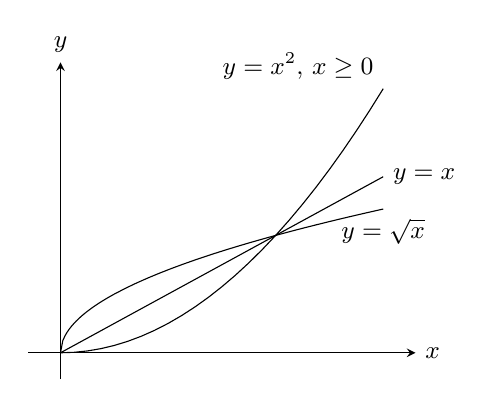
\begin{tikzpicture}[font=\small,declare function={f(\x)=\x^2;g(\x)=sqrt(\x);h(\x)=\x;}]
\begin{axis}[clip=false,small,axis lines=middle,enlargelimits=true,xlabel={$x$},ylabel={$y$},xlabel style={at={(current axis.right of origin)},anchor=west},ylabel style={at={(current axis.above origin)},anchor=south},xtick={\empty},ytick={\empty}]
\addplot[domain=0:1.5]{f(x)}node[above left]{$y=x^2,\, x\ge 0$};
\addplot[domain=0:0.25]{g(x)};
\addplot[domain=0.25:1.5]{g(x)}node[below]{$y=\sqrt{x}$};
\addplot[domain=0:1.5]{h(x)}node[right]{$y=x$};
\end{axis}
\end{tikzpicture}
\caption{
تفاعل \عددی{y=\sqrt{x}} اور \عددی{y=x^2,\, x\ge 0} ایک دوسرے کے الٹ ہیں (مثال \حوالہ{مثال_ماورائی_الٹ_تفاعل_کی_مثال})۔
}
\label{شکل_ماورائی_الٹ_تفاعل_تعریف}
\end{minipage}\hfill
\begin{minipage}{0.45\textwidth}
\centering
\begin{tikzpicture}[font=\small,declare function={f(\x)=1+3*(\x-1);g(\x)=\x;}]
\begin{axis}[clip=false,small,axis lines=middle,enlargelimits=true,xlabel={$x$},ylabel={$y$},xlabel style={at={(current axis.right of origin)},anchor=west},ylabel style={at={(current axis.above origin)},anchor=south},xtick={\empty},ytick={\empty}]
\addplot[domain=-0.25:2.25]{f(x)}node[above,align=left,xshift=3ex]{$y=\tfrac{1}{m}x-\tfrac{b}{m}$\\ ڈھلوان $\tfrac{1}{m}$};
\addplot[domain=0.25:3]({f(x)},x)node[pos=0.85,below,align=center,xshift=1ex]{$y=mx+b$\\ ڈھلوان m};
\addplot[domain=-0.5:5]{g(x)}node[right]{$y=x$};
\end{axis}
\end{tikzpicture}
\caption{
لکیر \عددی{y=x} میں منعکس غیر انتصابی لکیروں کے ڈھلوان ایک دوسرے کے بالعکس متناسب ہوتے ہیں۔
}
\label{شکل_ماورائی_عکس_میں_تفرق_تعلق}
\end{minipage}
\end{figure}


\جزوحصہء{قابل تفرق تفاعل کے الٹ کے تفرق}
تفاعل \عددی{f(x)=\tfrac{x}{2}+1}  اور اس کے الٹ \عددی{f^{-1}(x)=2x-2} (مثال \حوالہ{مثال_ماورائی_الٹ}) کے تفرق درج ذیل ہیں۔
\begin{align*}
\frac{\dif}{\dif x}f(x)&=\frac{\dif}{\dif x}\big(\frac{x}{2}+1\big)=\frac{1}{2}\\
\frac{\dif}{\dif x}f^{-1}(x)&=\frac{\dif}{\dif x}(2x-2)=2
\end{align*}
یہ تفرقات ایک دوسرے کے بالعکس متناسب ہیں۔ تفاعل \عددی{f} کی ترسیم لکیر \عددی{y=\tfrac{x}{2}+1} اور \عددی{f^{-1}} کی ترسیم لکیر \عددی{y=2x-2} ہے۔ ان لکیروں کے ڈھلوان ایک دوسرے کے بالعکس متناسب ہیں (شکل \حوالہ{شکل_ماورائی_عکس_میں_تفرق_تعلق})۔

یہ نتیجہ کسی مخصوص تفاعل کے لئے نہیں ہے۔ لکیر \عددی{y=x} میں کسی بھی غیر افقی یا غیر انتصابی لکیر کے عکس کا ڈھلوان اس لکیر کے ڈھلوان کے بالعکس متناسب ہو گا۔ یوں اگر دیے گئے لکیر کا ڈھلوان \عددی{m\ne 0} (شکل \حوالہ{شکل_ماورائی_عکس_میں_تفرق_تعلق}) ہو تب منعکس لکیر کا ڈھلوان \عددی{\tfrac{1}{m}} ہو گا۔ 

تفاعل اور اس کے الٹ کے ڈھلوانوں  کا بالعکس متناسب تعلق دیگر تفاعل کو بھی مطمئن کرتا ہے۔ اگر نقطہ \عددی{(a,f(a))} پر \عددی{y=f(x)} کا ڈھلوان \عددی{f'(a)\ne 0} ہو تب مطابقتی نقطہ \عددی{(f(a),a)} پر \عددی{y=f^{-1}(x)} کا ڈھلوان \عددی{\tfrac{1}{f'(a)}} ہو گا (شکل \حوالہ{شکل_ماورائی_ڈھلوان_بالعکس_متناسب})۔ یوں نقطہ \عددی{f(a)} پر \عددی{f^{-1}} کا تفرق، نقطہ \عددی{a} پر \عددی{f} کے تفرق کا بالعکس متناسب ہو گا۔ یہ تعلق اس صورت درست ہو گا جب \عددی{f} درج ذیل مسئلہ میں پیش   شرائط کو مطمئن کرتا ہو۔ یہ شرائط اعلٰی احصاء سے حاصل ہوتے ہیں۔ 

\begin{figure}
\centering
\begin{subfigure}{0.45\textwidth}
\centering
\begin{tikzpicture}[font=\small,declare function={f(\x)=(\x-1)^2;g(\x)=1+sqrt(\x);ta(\x)=9/16+3/2*(\x-7/4);}]
\pgfmathsetmacro{\a}{1.75}
\pgfmathsetmacro{\b}{f(\a)}
\begin{axis}[clip=false,small,axis lines=middle,enlargelimits=true,xlabel={$x$},ylabel={$y$},xlabel style={at={(current axis.right of origin)},anchor=west},ylabel style={at={(current axis.above origin)},anchor=south},xtick={\a}, xticklabels={$a$}, ytick={\b}, yticklabels={$f(a)$}]
\addplot[domain=1:2.2]{f(x)}node[above left]{$y=f(x)$};
%\addplot[domain=0:0.5]{g(x)};
%\addplot[domain=0.5:1.5]{g(x)};
\draw(\a,\b)node[circ]{}node[right,yshift=-1ex]{$(a,f(a))$};
%\draw(\b,\a)node[circ]{};
\addplot[domain=1.25:2.2]{ta(x)};
%\addplot[domain=1.25:2.25]({ta(x)},x);
\end{axis}
\end{tikzpicture}
\end{subfigure}\hfill
\begin{subfigure}{0.45\textwidth}
\centering
\begin{tikzpicture}[font=\small,declare function={f(\x)=(\x-1)^2;g(\x)=1+sqrt(\x);ta(\x)=9/16+3/2*(\x-7/4);}]
\pgfmathsetmacro{\a}{1.75}
\pgfmathsetmacro{\b}{f(\a)}
\begin{axis}[clip=false,small,axis lines=middle,enlargelimits=true,xlabel={$x$},ylabel={$y$},xlabel style={at={(current axis.right of origin)},anchor=west},ylabel style={at={(current axis.above origin)},anchor=south},xtick={\b},xticklabels={$f(a)$},ytick={\a},yticklabels={$a$}]
%\addplot[domain=1:2.2]{f(x)};
\addplot[domain=0:0.5]{g(x)};
\addplot[domain=0.5:1.5]{g(x)}node[pos=0.75,below right]{$y=f^{-1}(x)$};
%\draw(\a,\b)node[circ]{};
\draw(\b,\a)node[circ]{}node[right,yshift=-1ex]{$(f(a),a)$};
%\addplot[domain=1:2.2]{ta(x)};
\addplot[domain=1.4:2.25]({ta(x)},x);
\end{axis}
\end{tikzpicture}
\end{subfigure}
\caption{
الٹ تفاعل کے مطابقتی نقطوں پر ڈھلوان ایک دوسرے کا بالعکس متناسب 
\عددی{\left.\tfrac{\dif f^{-1}}{\dif x}\right\vert_{f(a)}=\tfrac{1}{\left.\tfrac{\dif f}{\dif x}\right\vert_{a}}} ہو گا۔
}
\label{شکل_ماورائی_ڈھلوان_بالعکس_متناسب}
\end{figure}
\ابتدا{مسئلہ}\شناخت{مسئلہ_ماورائی_الٹ_تفرق_قاعدہ}\موٹا{الٹ تفاعل کے تفرق کا قاعدہ}\\
اگر وقفہ \عددی{I} کے ہر نقطہ پر \عددی{f} قابل تفرق ہو اور \عددی{I} پر \عددی{\tfrac{\dif f}{\dif x}} کبھی بھی صفر  نہ ہو، تب وقفہ \عددی{f(I)} کے ہر نقطہ پر \عددی{f^{-1}} قابل تفرق ہو گا۔ کسی ایک مخصوص نقطہ \عددی{f(a)} پر \عددی{\tfrac{\dif f^{-1}}{\dif x}} کا تفرق نقطہ \عددی{a} پر تفرق \عددی{\tfrac{\dif f}{\dif x}} کا بالعکس متناسب ہو گا:
\begin{align}\label{مساوات_ماورائی_قاعدہ_الٹ_تفرق_الف}
\big(\frac{\dif f^{-1}}{\dif x}\big)_{x=f(a)}=\frac{1}{\big(\frac{\dif f}{\dif x}\big)_{x=a}}
\end{align}
اس کو مختصراً درج ذیل لکھا جا سکتا ہے۔
\begin{align}\label{مساوات_ماورائی_قاعدہ_الٹ_تفرق_ب}
(f^{-1})'=\frac{1}{f'}
\end{align}
\انتہا{مسئلہ}
%==================

\ابتدا{مثال}\شناخت{مثال_ماورائی_تفرق_الٹ_تفرق}
تفاعل \عددی{f(x)=x^2,\,x\ge 0} اور اس کے الٹ \عددی{f^{-1}(x)=\sqrt{x}} کے لئے درج ذیل لکھا جا سکتا ہے۔
\begin{align*}
\frac{\dif f}{\dif x}=\frac{\dif}{\dif x}(x^2)=2x,\quad \frac{\dif f^{-1}}{\dif x}=\frac{\dif}{\dif x}\sqrt{x}=\frac{1}{2\sqrt{x}},\,\,x>0
\end{align*}
نقطہ \عددی{(4,2)} لکیر \عددی{y=x} کی دوسری طرف نقطہ \عددی{(2,4)} کا عکس ہے (شکل \حوالہ{شکل_مثال_ماورائی_تفرق_الٹ_تفرق})۔ان نقطوں پر درج ذیل حاصل ہو گا۔
\begin{align*}
\frac{\dif f}{\dif x}&=2x=2(2)=4&&\text{\RL{نقطہ $(2,4)$ پر}}\\
\frac{\dif f^{-1}}{\dif x}&=\frac{1}{2\sqrt{x}}=\frac{1}{2\sqrt{4}}=\frac{1}{4}=\frac{1}{\dif f/\dif x}&&\text{\RL{نقطہ $(4,2)$ پر}}
\end{align*}
\انتہا{مثال}
%====================
\begin{figure}
\centering
\begin{minipage}{0.45\textwidth}
\centering
\begin{tikzpicture}[font=\small,declare function={f(\x)=\x^2;ta(\x)=4+4*(\x-2);tb(\x)=2+1/4*(\x-4);}]
\begin{axis}[clip=false,small,axis lines=middle,enlargelimits=true,xlabel={$x$},ylabel={$y$},xlabel style={at={(current axis.right of origin)},anchor=west},ylabel style={at={(current axis.above origin)},anchor=south},xtick={2,4},ytick={2,4}]
\addplot[domain=0:2.5]{f(x)}node[above,xshift=3ex]{$y=x^2,\, x \ge 0$};
\addplot[domain=0:3]({f(x)},{x})node[below]{$y=\tfrac{1}{\sqrt{x}}$};
\addplot[thick,domain=1.5:2.5]{ta(x)};
\addplot[thick,domain=2.5:8]{tb(x)};
\draw(2,4)node[circ]{}node[left]{$(2,4)$}node[right]{ڈھلوان 4};
\draw(4,2)node[circ]{}node[below]{$(4,2)$}node[above]{ڈھلوان $\tfrac{1}{4}$};
\end{axis}
\end{tikzpicture}
\caption{
نقطہ \عددی{(4,2)} پر \عددی{f^{-1}(x)=\sqrt{x}} کا تفرق نقطہ \عددی{(2,4)} پر \عددی{f(x)=x^2} کے تفرق کا بالعکس متناسب ہو گا (مثال \حوالہ{مثال_ماورائی_تفرق_الٹ_تفرق})۔
}
\label{شکل_مثال_ماورائی_تفرق_الٹ_تفرق}
\end{minipage}\hfill
\begin{minipage}{0.45\textwidth}
\centering
\begin{tikzpicture}[font=\small,declare function={f(\x)=\x^3-2;g(\x)=(\x+2)^(1/3); ta(\x)=6+12*(\x-2);tb(\x)=2+1/12*(\x-6);}]
\begin{axis}[clip=false,small,axis lines=middle,enlargelimits=true,xlabel={$x$},ylabel={$y$},xlabel style={at={(current axis.right of origin)},anchor=west},ylabel style={at={(current axis.above origin)},anchor=south},xtick={-2,6},ytick={-2,6}]
\addplot[domain=0:2.05]{f(x)}node[above,xshift=3ex]{$y=x^3-2$};
\addplot[domain=-2:-1.5]{g(x)};
\addplot[domain=-1.5:7]{g(x)};
\addplot[thick,domain=1.75:2.05]{ta(x)};
\addplot[thick,domain=3:7]{tb(x)};
\draw(2,6)node[circ]{}node[left]{$(2,6)$}node[right]{ڈھلوان 12};
\draw(6,2)node[circ]{}node[below]{$(6,2)$}node[above]{الٹ ڈھلوان $\tfrac{1}{12}$};
\end{axis}
\end{tikzpicture}
\caption{
نقطہ \عددی{x=2} پر \عددی{f(x)=x^3-2} کا تفرق ہمیں نقطہ \عددی{x=6} پر \عددی{f^{-1}} کا تفرق دیتا  ہے (مثال \حوالہ{مثال_ماورائی_ایک_نقطہ_پر_تفرق_سے_الٹ_تفرق_کا_حصول})۔
}
\label{شکل_مثال_ماورائی_ایک_نقطہ_پر_تفرق_سے_الٹ_تفرق_کا_حصول}
\end{minipage}
\end{figure}

بعض اوقات \عددی{f^{-1}} کا کلیہ نہ جانتے ہوئے بھی مساوات \حوالہ{مساوات_ماورائی_قاعدہ_الٹ_تفرق_الف} کی مدد سے \عددی{\tfrac{\dif f^{-1}}{\dif x}} کی مخصوص قیمتیں تلاش کی جا سکتی ہیں۔

\ابتدا{مثال}\شناخت{مثال_ماورائی_ایک_نقطہ_پر_تفرق_سے_الٹ_تفرق_کا_حصول}
مان لیں \عددی{f(x)=x^3-2} ہے۔ \عددی{f^{-1}(x)} کا کلیہ دریافت کیے بغیر نقطہ \عددی{x=6=f(2)} پر \عددی{\tfrac{\dif f^{-1}}{\dif x}} کی قیمت تلاش کریں۔

حل:  (شکل \حوالہ{شکل_مثال_ماورائی_ایک_نقطہ_پر_تفرق_سے_الٹ_تفرق_کا_حصول})
\begin{align*}
\left.\frac{\dif f}{\dif x}\right\vert_{x=2}&=\left.3x^2\right\vert_{x=2}=12\\
\left.\frac{\dif f^{-1}}{\dif x}\right\vert_{x=f(2)}&=\frac{1}{12}&&\text{\RL{مساوات \حوالہ{مساوات_ماورائی_قاعدہ_الٹ_تفرق_الف}}}
\end{align*}
\انتہا{مثال}
%=======================

مسئلہ \حوالہ{مسئلہ_ماورائی_الٹ_تفرق_قاعدہ} کو ایک مختلف نقطہ نظر سے دیکھا جا سکتا ہے۔ اگر \عددی{x=a} پر \عددی{y=f(x)}  قابل تفرق ہو اور ہم \عددی{x} کی قیمت میں معمولی تبدیلی \عددی{\dif x} لائیں تب \عددی{y} میں مطابقتی تبدیلی تخمیناً
\begin{align*}
\dif y=f'(a)\dif x
\end{align*}
ہو گا۔اس کا مطلب ہے کہ \عددی{y} کی تبدیلی، \عددی{x} کی تبدیلی کے تقریباً \عددی{f'(a)} گنّا ہو گی اور \عددی{x} کی تبدیلی، \عددی{y} کی تبدیلی کے تقریباً  \عددی{\tfrac{1}{f'(a)}} گنّا ہو گی۔

\حصہء{سوالات}
\موٹا{ایک ایک تفاعل کی نشاندہی}\\
سوال \حوالہ{سوال_ماورائی_ایک_ایک_نشاندہی_الف} تا سوال \حوالہ{سوال_ماورائی_ایک_ایک_نشاندہی_ث} میں تفاعل کے ترسیم دیے گئے ہیں۔ ان میں  ایک ایک تفاعل کی نشاندہی کریں۔

\ابتدا{سوال}\شناخت{سوال_ماورائی_ایک_ایک_نشاندہی_الف}
ترسیم شکل \حوالہ{شکل_سوال_ماورائی_ایک_ایک_نشاندہی_الف} میں دی گئی ہے۔\\
جواب:\quad
ایک ایک
\انتہا{سوال}
%=======================
\ابتدا{سوال}\شناخت{سوال_ماورائی_ایک_ایک_نشاندہی_ب}
ترسیم شکل \حوالہ{شکل_سوال_ماورائی_ایک_ایک_نشاندہی_ب} میں دی گئی ہے۔
\انتہا{سوال}
%=======================
\ابتدا{سوال}\شناخت{سوال_ماورائی_ایک_ایک_نشاندہی_پ}
ترسیم شکل \حوالہ{شکل_سوال_ماورائی_ایک_ایک_نشاندہی_پ} میں دی گئی ہے۔\\
جواب:\quad
غیر ایک ایک
\انتہا{سوال}
%=======================
\ابتدا{سوال}\شناخت{سوال_ماورائی_ایک_ایک_نشاندہی_ت}
ترسیم شکل \حوالہ{شکل_سوال_ماورائی_ایک_ایک_نشاندہی_ت} میں دی گئی ہے۔
\انتہا{سوال}
%=======================
\ابتدا{سوال}\شناخت{سوال_ماورائی_ایک_ایک_نشاندہی_ٹ}
ترسیم شکل \حوالہ{شکل_سوال_ماورائی_ایک_ایک_نشاندہی_ٹ} میں دی گئی ہے۔\\
جواب:\quad
ایک ایک
\انتہا{سوال}
%=======================
\ابتدا{سوال}\شناخت{سوال_ماورائی_ایک_ایک_نشاندہی_ث}
ترسیم شکل \حوالہ{شکل_سوال_ماورائی_ایک_ایک_نشاندہی_ث} میں دی گئی ہے۔
\انتہا{سوال}
%=================
\begin{figure}
\centering
\begin{minipage}{0.3\textwidth}
\centering
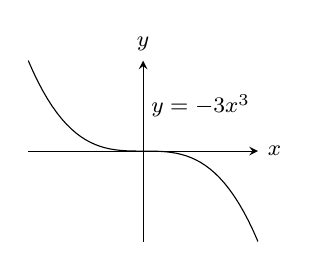
\begin{tikzpicture}[font=\footnotesize,declare function={f(\x)=-3*\x^3;}]
\begin{axis}[width=4.5cm,axis lines=middle,xlabel={$x$},ylabel={$y$},xlabel style={at={(current axis.right of origin)},anchor=west},ylabel style={at={(current axis.above origin)},anchor=south},xtick={\empty},ytick={\empty}]
\addplot[domain=0:2]{f(x)};
\addplot[domain=0:2]({-x},{-f(x)});
\draw(1,{-1/2*f(2)})node[]{$y=-3x^3$};
\end{axis}
\end{tikzpicture}
\caption{ترسیم سوال \حوالہ{سوال_ماورائی_ایک_ایک_نشاندہی_الف}}
\label{شکل_سوال_ماورائی_ایک_ایک_نشاندہی_الف}
\end{minipage}\hfill
\begin{minipage}{0.3\textwidth}
\centering
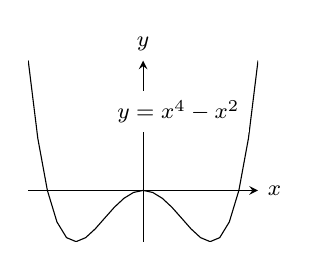
\begin{tikzpicture}[font=\footnotesize,declare function={f(\x)=\x^4-\x^2;}]
\begin{axis}[width=4.5cm,axis lines=middle,xlabel={$x$},ylabel={$y$},xlabel style={at={(current axis.right of origin)},anchor=west},ylabel style={at={(current axis.above origin)},anchor=south},xtick={\empty},ytick={\empty}]
\addplot[domain=-1.2:1.2]{f(x)}node[pos=0.9,above left,fill=white]{$y=x^4-x^2$};
\end{axis}
\end{tikzpicture}
\caption{ترسیم سوال \حوالہ{سوال_ماورائی_ایک_ایک_نشاندہی_ب}}
\label{شکل_سوال_ماورائی_ایک_ایک_نشاندہی_ب}
\end{minipage}\hfill
\begin{minipage}{0.3\textwidth}
\centering
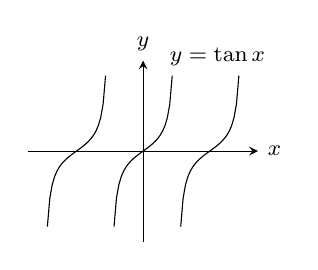
\begin{tikzpicture}[font=\footnotesize,declare function={f(\x)=tan(deg(\x));}]
\begin{axis}[clip=false,width=4.5cm,axis lines=middle,xlabel={$x$},ylabel={$y$},xlabel style={at={(current axis.right of origin)},anchor=west},ylabel style={at={(current axis.above origin)},anchor=south},xtick={\empty},ytick={\empty},enlargelimits=true]
\addplot[domain=-3/2*pi+0.2:-pi/2-0.2]{f(x)};
\addplot[domain=-pi/2+0.2:pi/2-0.2]{f(x)};
\addplot[domain=pi/2+0.2:3/2*pi-0.2]{f(x)}node[above  left,xshift=3ex]{$y=\tan x$};
\end{axis}
\end{tikzpicture}
\caption{ترسیم سوال \حوالہ{سوال_ماورائی_ایک_ایک_نشاندہی_پ}}
\label{شکل_سوال_ماورائی_ایک_ایک_نشاندہی_پ}
\end{minipage}
\end{figure}
%======================
\begin{figure}
\centering
\begin{minipage}{0.3\textwidth}
\centering
\begin{tikzpicture}[font=\footnotesize,declare function={f(\x)=-3*\x^3;}]
\pgfmathsetmacro{\k}{1.25/5}
\draw[-latex](-1.25,0)--(1.25,0)node[right]{$x$};
\draw[-latex](0,-1.25)--(0,1.25)node[above]{$y$};
\foreach \x in {-1,-2,-3,-4,0,1,2,3}{\draw(\x*\k,\x*\k)node[circ]{}--++(\k,0)node[ocirc]{};}
\draw(-0.75,0.75)node[]{$y=\lfloor x\rfloor$};
\end{tikzpicture}
\caption{ترسیم سوال \حوالہ{سوال_ماورائی_ایک_ایک_نشاندہی_ت}}
\label{شکل_سوال_ماورائی_ایک_ایک_نشاندہی_ت}
\end{minipage}\hfill
\begin{minipage}{0.3\textwidth}
\centering
\begin{tikzpicture}[font=\footnotesize,declare function={f(\x)=1/\x;}]
\begin{axis}[width=4.5cm,axis lines=middle,xlabel={$x$},ylabel={$y$},xlabel style={at={(current axis.right of origin)},anchor=west},ylabel style={at={(current axis.above origin)},anchor=south},xtick={\empty},ytick={\empty}]
\addplot[domain=0.2:5]{f(x)}node[pos=0.25,right]{$y=\tfrac{1}{x}$};
\addplot[domain=0.2:5](-x,{-f(x)});
\end{axis}
\end{tikzpicture}
\caption{ترسیم سوال \حوالہ{سوال_ماورائی_ایک_ایک_نشاندہی_ٹ}}
\label{شکل_سوال_ماورائی_ایک_ایک_نشاندہی_ٹ}
\end{minipage}\hfill
\begin{minipage}{0.3\textwidth}
\centering
\begin{tikzpicture}[font=\footnotesize,declare function={f(\x)=\x^(1/3);}]
\begin{axis}[clip=false,width=4.5cm,axis lines=middle,xlabel={$x$},ylabel={$y$},xlabel style={at={(current axis.right of origin)},anchor=west},ylabel style={at={(current axis.above origin)},anchor=south},xtick={\empty},ytick={\empty},enlargelimits=true]
\addplot[domain=0:6]{f(x)};
\draw (-3,1)node[]{$y=x^{1/3}$};
\addplot[domain=0:6](-x,{-f(x)});
\end{axis}
\end{tikzpicture}
\caption{ترسیم سوال \حوالہ{سوال_ماورائی_ایک_ایک_نشاندہی_ث}}
\label{شکل_سوال_ماورائی_ایک_ایک_نشاندہی_ث}
\end{minipage}
\end{figure}

\موٹا{الٹ تفاعل کی ترسیم}\\
سوال \حوالہ{سوال_ماورائی_ترسیم_دیا_الف} تا سوال \حوالہ{سوال_ماورائی_ترسیم_دیا_ت} میں \عددی{y=f(x)} کی ترسیم دی گئی ہے۔ اس کو نقل کر کے لکیر  \عددی{y=x} بھی بنائیں۔ لکیر \عددی{y=x} کے لحاظ سے تشاکلی استعمال کرتے ہوئے \عددی{y=f^{-1}(x)} ترسیم کریں۔(\عددی{f^{-1}} کا کلیہ معلوم کرنے کی ضرورت نہیں ہے۔) \عددی{f^{-1}} کے دائرہ کار اور سعت کی نشاندہی  کریں۔

\ابتدا{سوال}\شناخت{سوال_ماورائی_ترسیم_دیا_الف}
تفاعل کی ترسیم شکل \حوالہ{شکل_سوال_ماورائی_ترسیم_دیا_الف} میں دی گئی ہے۔\\
جواب:\quad
دائرہ کار \عددی{(0,1]}، سعت \عددی{[0,\infty)}، شکل \حوالہ{شکل_جواب_ماورائی_ترسیم_دیا_الف}
\انتہا{سوال}
%=======================
\ابتدا{سوال}\شناخت{سوال_ماورائی_ترسیم_دیا_ب}
تفاعل کی ترسیم شکل \حوالہ{شکل_سوال_ماورائی_ترسیم_دیا_ب} میں دی گئی ہے۔
\انتہا{سوال}
%=======================
\ابتدا{سوال}\شناخت{سوال_ماورائی_ترسیم_دیا_پ}
تفاعل کی ترسیم شکل \حوالہ{شکل_سوال_ماورائی_ترسیم_دیا_پ} میں دی گئی ہے۔\\
جواب:\quad
دائرہ کار \عددی{[-1,1]}، سعت \عددی{-\tfrac{\pi}{2},\tfrac{\pi}{2}} ،شکل \حوالہ{شکل_جواب_ماورائی_ترسیم_دیا_پ}
\انتہا{سوال}
%=======================
\ابتدا{سوال}\شناخت{سوال_ماورائی_ترسیم_دیا_ت}
تفاعل کی ترسیم شکل \حوالہ{شکل_سوال_ماورائی_ترسیم_دیا_ت} میں دی گئی ہے۔
\انتہا{سوال}
%=======================
\begin{figure}
\centering
\begin{minipage}{0.2\textwidth}
\centering
\begin{tikzpicture}[font=\tiny,declare function={f(\x)=1/(\x^2+1);}]
\begin{axis}[clip=false,width=4cm,axis lines=middle,xlabel={$x$},ylabel={$y$},xlabel style={at={(current axis.right of origin)},anchor=west},ylabel style={at={(current axis.above origin)},anchor=south},xtick={1},ytick={1},enlargelimits=true,ymin=0]
\addplot[domain=0:2]{f(x)}node[pos=0.5,above right]{$\begin{aligned}y&=f(x)\\ &=\frac{1}{\x^2+1},\, x\ge 0\end{aligned}$};
\end{axis}
\end{tikzpicture}
\caption{ترسیم سوال \حوالہ{سوال_ماورائی_ترسیم_دیا_الف}}
\label{شکل_سوال_ماورائی_ترسیم_دیا_الف}
\end{minipage}\hfill
\begin{minipage}{0.2\textwidth}
\centering
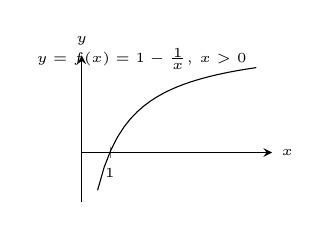
\begin{tikzpicture}[font=\tiny,declare function={f(\x)=1-1/\x;}]
\begin{axis}[clip=false,width=4cm,axis lines=middle,xlabel={$x$},ylabel={$y$},xlabel style={at={(current axis.right of origin)},anchor=west},ylabel style={at={(current axis.above origin)},anchor=south},xtick={1},ytick={1},enlargelimits=true]
\addplot[domain=0.75:4]{f(x)}node[pos=1,above left,yshift=-1ex]{$y=f(x)=1-\frac{1}{x},\, x> 0$};
\end{axis}
\end{tikzpicture}
\caption{ترسیم سوال \حوالہ{سوال_ماورائی_ترسیم_دیا_ب}}
\label{شکل_سوال_ماورائی_ترسیم_دیا_ب}
\end{minipage}\hfill
\begin{minipage}{0.2\textwidth}
\centering
\begin{tikzpicture}[font=\tiny,declare function={f(\x)=sin(deg(\x));}]
\pgfmathsetmacro{\k}{1/2*pi}
\begin{axis}[clip=false,width=4cm,axis lines=middle,xlabel={$x$},ylabel={$y$},xlabel style={at={(current axis.right of origin)},anchor=west},ylabel style={at={(current axis.above origin)},anchor=south},xtick={-\k,\k},xticklabels={$-\tfrac{\pi}{2}$,$\tfrac{\pi}{2}$},ytick={-1,1},enlargelimits=true]
\addplot[domain=-1/2*pi:1/2*pi]{f(x)};
\draw(-1/2*pi,1)node[]{$\begin{aligned}y&=f(x)=\sin x\\  &-\tfrac{\pi}{2}\le x\le \tfrac{\pi}{2}\end{aligned}$};
\draw(-\k,-1)node[circ]{}  (\k,1)node[circ]{};
\end{axis}
\end{tikzpicture}
\caption{ترسیم سوال \حوالہ{سوال_ماورائی_ترسیم_دیا_پ}}
\label{شکل_سوال_ماورائی_ترسیم_دیا_پ}
\end{minipage}\hfill
\begin{minipage}{0.2\textwidth}
\centering
\begin{tikzpicture}[font=\tiny,declare function={f(\x)=tan(deg(\x));}]
\pgfmathsetmacro{\k}{1/2*pi}
\begin{axis}[clip=false,width=4cm,axis lines=middle,xlabel={$x$},ylabel={$y$},xlabel style={at={(current axis.right of origin)},anchor=west},ylabel style={at={(current axis.above origin)},anchor=south}, xtick={-\k,\k},  xticklabels={$-\tfrac{\pi}{2}$,$\tfrac{\pi}{2}$}, ytick={\empty},xmin=-\k-0.1,xmax=\k+0.2]
\addplot[domain=-\k+0.4:\k-0.4]{f(x)};
\draw(-1/2*pi,2)node[]{$\begin{aligned}y&=f(x)=\tan x\\  &-\tfrac{\pi}{2}< x<\tfrac{\pi}{2}\end{aligned}$};
\end{axis}
\end{tikzpicture}
\caption{ترسیم سوال \حوالہ{سوال_ماورائی_ترسیم_دیا_ت}}
\label{شکل_سوال_ماورائی_ترسیم_دیا_ت}
\end{minipage}
\end{figure}
%
\begin{figure}
\centering
\begin{minipage}{0.3\textwidth}
\centering
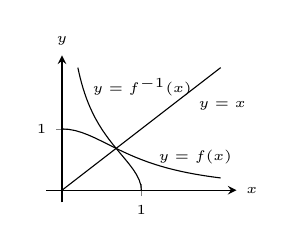
\begin{tikzpicture}[font=\tiny,declare function={f(\x)=1/(\x^2+1);m(\x)=\x;}]
\begin{axis}[clip=false,width=4cm,axis lines=middle,xlabel={$x$},ylabel={$y$},xlabel style={at={(current axis.right of origin)},anchor=west},ylabel style={at={(current axis.above origin)},anchor=south},xtick={1},ytick={1},enlargelimits=true,ymin=0]
\addplot[domain=0:2]{f(x)}node[pos=0.85,above]{$y=f(x)$};
\addplot[domain=0:2]({f(x)},x)node[pos=0.85,right]{$y=f^{-1}(x)$};
\addplot[domain=0:2]{m(x)}node[pos=0.8,below right]{$y=x$};
\end{axis}
\end{tikzpicture}
\caption{ترسیم جواب \حوالہ{سوال_ماورائی_ترسیم_دیا_الف}}
\label{شکل_جواب_ماورائی_ترسیم_دیا_الف}
\end{minipage}\hfill
\begin{minipage}{0.3\textwidth}
\centering
\begin{tikzpicture}[font=\tiny,declare function={f(\x)=sin(deg(\x));m(\x)=\x;}]
\pgfmathsetmacro{\k}{1/2*pi}
\begin{axis}[clip=false,width=4cm,axis lines=middle,xlabel={$x$},ylabel={$y$},xlabel style={at={(current axis.right of origin)},anchor=west},ylabel style={at={(current axis.above origin)},anchor=south},xtick={-\k,\k},xticklabels={$-\tfrac{\pi}{2}$,$\tfrac{\pi}{2}$},ytick={-1,1},enlargelimits=true]
\addplot[domain=-1/2*pi:1/2*pi]{f(x)}node[right]{$y=f(x)$};
\addplot[domain=-1/2*pi:1/2*pi]({f(x)},x)node[above]{$y=f^{-1}(x)$};
\addplot[domain=-1/2*pi:1/2*pi]{m(x)}node[right]{$y=x$};
%\draw(-1/2*pi,1)node[]{$\begin{aligned}y&=f(x)=\sin x\\  &-\tfrac{\pi}{2}\le x\le \tfrac{\pi}{2}\end{aligned}$};
\end{axis}
\end{tikzpicture}
\caption{ترسیم جواب \حوالہ{سوال_ماورائی_ترسیم_دیا_پ}}
\label{شکل_جواب_ماورائی_ترسیم_دیا_پ}
\end{minipage}\hfill
\begin{minipage}{0.3\textwidth}
\centering
\begin{tikzpicture}[font=\tiny,declare function={f(\x)=sqrt(1-\x^2);m(\x)=\x;}]
\pgfmathsetmacro{\k}{1/2*pi}
\begin{axis}[clip=false,width=4cm,axis lines=middle,xlabel={$x$},ylabel={$y$},xlabel style={at={(current axis.right of origin)},anchor=west},ylabel style={at={(current axis.above origin)},anchor=south},xtick={1},ytick={1},enlargelimits=true]
\addplot[domain=0:0.9]{f(x)}node[pos=0.5,above right]{$\begin{aligned}y&=f(x)\\  0&\le x\le 1\end{aligned}$};
\addplot[domain=0.9:1]{f(x)};
\end{axis}
\end{tikzpicture}
\caption{ترسیم جواب \حوالہ{سوال_ماورائی_تشاکلی_دریافت_الف}}
\label{شکل_جواب_ماورائی_تشاکلی_دریافت_الف}
\end{minipage}
\end{figure}

\ابتدا{سوال}\شناخت{سوال_ماورائی_تشاکلی_دریافت_الف}
(ا) تفاعل \عددی{f(x)=\sqrt{1-x^2},\, 0\le x\le 1} ترسیم کریں۔ اس ترسیم میں کون سی تشاکلی پائی جاتی ہے؟ (ب) دکھائیں کہ \عددی{f} اپنا ہی الٹ ہے۔ (یاد رہے کہ \عددی{x\ge 0} کی صورت میں \عددی{\sqrt{x^2}=x} ہوتا ہے۔)\\
جواب:\quad
لکیر \عددی{y=x} کے لحاظ سے تشاکلی ہے۔ شکل \حوالہ{شکل_جواب_ماورائی_تشاکلی_دریافت_الف}
\انتہا{سوال}
%==============
\ابتدا{سوال}
(ا) تفاعل \عددی{f(x)=\tfrac{1}{x}} ترسیم کریں۔ اس ترسیم میں کون سی تشاکلی پائی جاتی ہے؟ (ب) دکھائیں کہ \عددی{f} اپنا ہی الٹ ہے۔
\انتہا{سوال}
%==================
\موٹا{الٹ تفاعل کے کلیات}\\
سوال \حوالہ{سوال_ماورائی_ترسیم_کلیہ_الف} تا سوال \حوالہ{سوال_ماورائی_ترسیم_کلیہ_ث} میں تفاعل \عددی{y=f(x)} کا کلیہ دیا گیا ہے۔ \عددی{f} اور \عددی{f^{-1}} کی ترسیمات بھی دکھائی گئی ہیں۔ \عددی{f^{-1}} کا کلیہ تلاش کریں۔

\ابتدا{سوال}\شناخت{سوال_ماورائی_ترسیم_کلیہ_الف}
$f(x)=x^2+1,\quad x\ge 0$
ترسیم شکل \حوالہ{شکل_سوال_ماورائی_ترسیم_کلیہ_الف} میں دی گئی ہے۔\\
جواب:\quad
$f^{-1}(x)=\sqrt{x-1}$
\انتہا{سوال}
%===================
\ابتدا{سوال}\شناخت{سوال_ماورائی_ترسیم_کلیہ_ب}
$f(x)=x^2,\quad x\le 0$
ترسیم شکل \حوالہ{شکل_سوال_ماورائی_ترسیم_کلیہ_ب} میں دی گئی ہے۔
\انتہا{سوال}
%===================
\ابتدا{سوال}\شناخت{سوال_ماورائی_ترسیم_کلیہ_پ}
$f(x)=x^3-1$
ترسیم شکل \حوالہ{شکل_سوال_ماورائی_ترسیم_کلیہ_پ} میں دی گئی ہے۔\\
جواب:\quad
$f^{-1}(x)=\sqrt[3]{x+1}$
\انتہا{سوال}
%===================
\ابتدا{سوال}\شناخت{سوال_ماورائی_ترسیم_کلیہ_ت}
$f(x)=x^2-2x+1,\quad x\ge 1$
ترسیم شکل \حوالہ{شکل_سوال_ماورائی_ترسیم_کلیہ_ت} میں دی گئی ہے۔
\انتہا{سوال}
%===================
\ابتدا{سوال}\شناخت{سوال_ماورائی_ترسیم_کلیہ_ٹ}
$f(x)=(x+1)^2,\quad x\ge -1$
ترسیم شکل \حوالہ{شکل_سوال_ماورائی_ترسیم_کلیہ_ٹ} میں دی گئی ہے۔\\
جواب:\quad
$f^{-1}(x)=\sqrt{x}-1$
\انتہا{سوال}
%===================
\ابتدا{سوال}\شناخت{سوال_ماورائی_ترسیم_کلیہ_ث}
$f(x)=x^{2/3},\quad x\ge 0$
ترسیم شکل \حوالہ{شکل_سوال_ماورائی_ترسیم_کلیہ_ث} میں دی گئی ہے۔
\انتہا{سوال}
%===================
\begin{figure}
\centering
\begin{minipage}{0.3\textwidth}
\centering
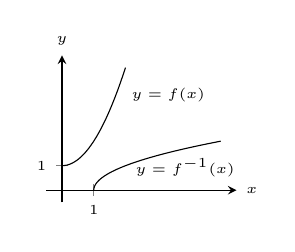
\begin{tikzpicture}[font=\tiny,declare function={f(\x)=\x^2+1;}]
\begin{axis}[clip=false,width=4cm,axis lines=middle,xlabel={$x$},ylabel={$y$},xlabel style={at={(current axis.right of origin)},anchor=west},ylabel style={at={(current axis.above origin)},anchor=south},xtick={1},ytick={1},enlargelimits=true,ymin=0]
\addplot[domain=0:2]{f(x)}node[pos=0.9,below right]{$y=f(x)$};
\addplot[domain=0:2]({f(x)},x)node[pos=0.75,below]{$y=f^{-1}(x)$};
\end{axis}
\end{tikzpicture}
\caption{ترسیم سوال \حوالہ{سوال_ماورائی_ترسیم_کلیہ_الف}}
\label{شکل_سوال_ماورائی_ترسیم_کلیہ_الف}
\end{minipage}\hfill
\begin{minipage}{0.3\textwidth}
\centering
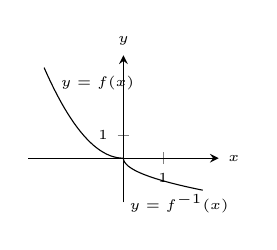
\begin{tikzpicture}[font=\tiny,declare function={f(\x)=\x^2;}]
\begin{axis}[clip=false,width=4cm,axis lines=middle,xlabel={$x$},ylabel={$y$},xlabel style={at={(current axis.right of origin)},anchor=west},ylabel style={at={(current axis.above origin)},anchor=south},xtick={1},ytick={1},enlargelimits=true]
\addplot[domain=0:2](-x,{f(x)})node[pos=0.85,right]{$y=f(x)$};
\addplot[domain=0:1.4142]({f(x)},-x)node[pos=0.75,below]{$y=f^{-1}(x)$};
\end{axis}
\end{tikzpicture}
\caption{ترسیم سوال \حوالہ{سوال_ماورائی_ترسیم_کلیہ_ب}}
\label{شکل_سوال_ماورائی_ترسیم_کلیہ_ب}
\end{minipage}\hfill
\begin{minipage}{0.3\textwidth}
\centering
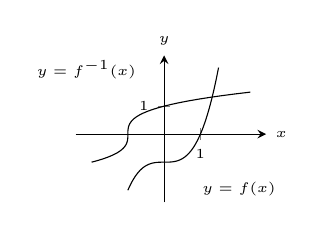
\begin{tikzpicture}[font=\tiny,declare function={f(\x)=\x^3-1;g(\x)=\x^3+1;}]
\begin{axis}[clip=false,width=4cm,axis lines=middle,xlabel={$x$},ylabel={$y$},xlabel style={at={(current axis.right of origin)},anchor=west},ylabel style={at={(current axis.above origin)},anchor=south},xtick={1},ytick={1},enlargelimits=true]
\addplot[domain=0:1.5]{f(x)}node[pos=0.25,below right,yshift={-2ex}]{$y=f(x)$};
\addplot[domain=0:1](-x,{-g(x)});
\addplot[domain=0:1.5]({f(x)},x)node[pos=0.25,above left,yshift=2ex]{$y=f^{-1}(x)$};
\addplot[domain=0:1]({-g(x)},-x);
\end{axis}
\end{tikzpicture}
\caption{ترسیم سوال \حوالہ{سوال_ماورائی_ترسیم_کلیہ_پ}}
\label{شکل_سوال_ماورائی_ترسیم_کلیہ_پ}
\end{minipage}
\end{figure}
%==============================
\begin{figure}
\centering
\begin{minipage}{0.3\textwidth}
\centering
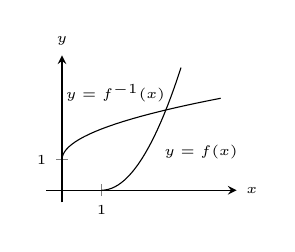
\begin{tikzpicture}[font=\tiny,declare function={f(\x)=\x^2-2*\x+1;}]
\begin{axis}[clip=false,width=4cm,axis lines=middle,xlabel={$x$},ylabel={$y$},xlabel style={at={(current axis.right of origin)},anchor=west},ylabel style={at={(current axis.above origin)},anchor=south},xtick={1},ytick={1},enlargelimits=true,ymin=0]
\addplot[domain=1:3]{f(x)}node[pos=0.5,below right]{$y=f(x)$};
\addplot[domain=1:3]({f(x)},x)node[pos=0.4,above,yshift=1ex]{$y=f^{-1}(x)$};
\end{axis}
\end{tikzpicture}
\caption{ترسیم سوال \حوالہ{سوال_ماورائی_ترسیم_کلیہ_ت}}
\label{شکل_سوال_ماورائی_ترسیم_کلیہ_ت}
\end{minipage}\hfill
\begin{minipage}{0.3\textwidth}
\centering
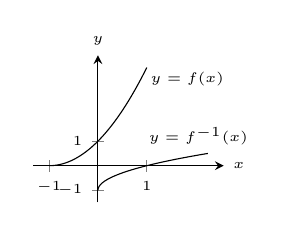
\begin{tikzpicture}[font=\tiny,declare function={f(\x)=(\x+1)^2;g(\x)=(\x-1)^2;}]
\begin{axis}[clip=false,width=4cm,axis lines=middle,xlabel={$x$},ylabel={$y$},xlabel style={at={(current axis.right of origin)},anchor=west},ylabel style={at={(current axis.above origin)},anchor=south},xtick={-1,1},ytick={-1,1},enlargelimits=true]
\addplot[domain=0:1](x,{f(x)})node[pos=0.85,right]{$y=f(x)$};
\addplot[domain=0:1](-x,{g(x)});
\addplot[domain=0:0.5]({f(x)},x)node[pos=0.85,above]{$y=f^{-1}(x)$};
\addplot[domain=0:1]({g(x)},-x);
\end{axis}
\end{tikzpicture}
\caption{ترسیم سوال \حوالہ{سوال_ماورائی_ترسیم_کلیہ_ٹ}}
\label{شکل_سوال_ماورائی_ترسیم_کلیہ_ٹ}
\end{minipage}\hfill
\begin{minipage}{0.3\textwidth}
\centering
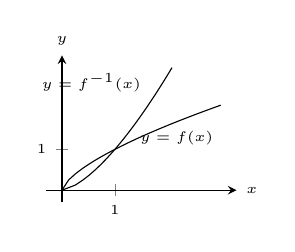
\begin{tikzpicture}[font=\tiny,declare function={f(\x)=(\x^2)^(1/3);}]
\begin{axis}[clip=false,width=4cm,axis lines=middle,xlabel={$x$},ylabel={$y$},xlabel style={at={(current axis.right of origin)},anchor=west},ylabel style={at={(current axis.above origin)},anchor=south},xtick={1},ytick={1},enlargelimits=true]
\addplot[domain=0:3]{f(x)}node[pos=0.75,below]{$y=f(x)$};
\addplot[domain=0:3]({f(x)},x)node[pos=0.75,above left,]{$y=f^{-1}(x)$};
\end{axis}
\end{tikzpicture}
\caption{ترسیم سوال \حوالہ{سوال_ماورائی_ترسیم_کلیہ_ث}}
\label{شکل_سوال_ماورائی_ترسیم_کلیہ_ث}
\end{minipage}
\end{figure}

سوال \حوالہ{سوال_ماورائی_تصدیق_الف} تا سوال \حوالہ{سوال_ماورائی_تصدیق_ب} میں تفاعل \عددی{y=f(x)} کا کلیہ دیا گیا ہے۔ \عددی{f^{-1}} دریافت کریں اور اس کے دائرہ کار اور سعت کی نشاندہی کریں۔ تصدیق کی خاطر دکھائیں کہ \عددی{f(f^{-1}(x))=f^{-1}(f(x))=x} ہے۔ 

\ابتدا{سوال}\شناخت{سوال_ماورائی_تصدیق_الف}
$f(x)=x^5$\\
جواب:\quad
$f^{-1}(x)=\sqrt[5]{x}$
 دائرہ کار \عددی{-\infty<x<\infty}، سعت \عددی{-\infty<y<\infty}
\انتہا{سوال}
%======================
\ابتدا{سوال}
$f(x)=x^4,\quad x\ge 0$
\انتہا{سوال}
%======================
\ابتدا{سوال}
$f(x)=x^3+1$\\
جواب:\quad
$f^{-1}(x)=\sqrt[3]{x-1}$
دائرہ کار \عددی{-\infty<x<\infty}، سعت \عددی{-\infty<y<\infty}
\انتہا{سوال}
%======================
\ابتدا{سوال}
$f(x)=\tfrac{x}{2}-\tfrac{7}{2}$
\انتہا{سوال}
%======================
\ابتدا{سوال}
$f(x)=\tfrac{1}{x^2},\quad x>0$\\
جواب:\quad
$f^{-1}(x)=\tfrac{1}{\sqrt{x}}$
دائرہ کار \عددی{x>0}، سعت \عددی{y>0}
\انتہا{سوال}
%======================
\ابتدا{سوال}\شناخت{سوال_ماورائی_تصدیق_ب}
$f(x)=\tfrac{1}{x^3},\quad x\ne 0$
\انتہا{سوال}
%======================
\موٹا{الٹ تفاعل کے تفرق}\\
سوال \حوالہ{سوال_ماورائی_تصدیق_تفرق_الف} تا سوال \حوالہ{سوال_ماورائی_تصدیق_تفرق_ب} میں درج ذیل اقدام کریں۔
\begin{enumerate}[a.]
\item
\عددی{f^{-1}(x)} تلاش کریں۔
\item
\عددی{f} اور \عددی{f^{-1}} کو ایک ساتھ ترسیم کریں۔
\item
نقطہ \عددی{x=a} پر \عددی{\tfrac{\dif f}{\dif x}} اور نقطہ \عددی{x=f(a)} پر \عددی{\tfrac{\dif f^{-1}}{\dif x}} کی قیمت حاصل کریں۔ تصدیق کریں کہ ان نقطوں پر \عددی{\tfrac{\dif f^{-1}}{\dif x}=\tfrac{1}{\big(\tfrac{\dif f}{\dif x}\big)}} ہو گا۔
\end{enumerate}

\ابتدا{سوال}\شناخت{سوال_ماورائی_تصدیق_تفرق_الف}
$f(x)=2x+3,\quad a=-1$\\
جواب:\quad
(ا) \عددی{f^{-1}(x)=\tfrac{x}{2}-\tfrac{3}{2}}، (ب) شکل \حوالہ{شکل_جواب_ماورائی_تصدیق_تفرق_الف}، (ج) \عددی{2,\tfrac{1}{2}}
\انتہا{سوال}
%============================
\ابتدا{سوال}
$f(x)=\tfrac{x}{5}+7,\quad a=-1$
\انتہا{سوال}
%============================
\ابتدا{سوال}\شناخت{سوال_ماورائی_تصدیق_تفرق_درکار_پ}
$f(x)=5-4x,\quad a=\tfrac{1}{2}$\\
جواب:\quad
(ا) \عددی{f^{-1}(x)=-\tfrac{x}{4}+\tfrac{5}{4}}، (ب) شکل \حوالہ{شکل_جواب_ماورائی_تصدیق_تفرق_درکار_پ}،  (ج) \عددی{-4,-\tfrac{1}{4}}
\انتہا{سوال}
%============================
\ابتدا{سوال}\شناخت{سوال_ماورائی_تصدیق_تفرق_ب}
$f(x)=2x^2,\quad x\ge 0,\quad a=5$
\انتہا{سوال}
%============================
\begin{figure}
\centering
\begin{minipage}{0.3\textwidth}
\centering
\begin{tikzpicture}[font=\tiny,declare function={f(\x)=2*\x+3;}]
\begin{axis}[clip=false,width=4cm,axis lines=middle,xlabel={$x$},ylabel={$y$},xlabel style={at={(current axis.right of origin)},anchor=west},ylabel style={at={(current axis.above origin)},anchor=south}, xtick={-1.5,3},xticklabels={$-\tfrac{3}{2}$,$3$},ytick={-1.5,3},yticklabels={$-\tfrac{3}{2}$,$3$}, enlargelimits=true]
\addplot[domain=-1.7:0.5]{f(x)}node[right]{$y=f(x)=2x+3$};
\addplot[domain=-1.7:0.5]({f(x)},x)node[above,]{$y=f^{-1}(x)=\tfrac{x}{2}-\tfrac{3}{2}$};
\end{axis}
\end{tikzpicture}
\caption{ترسیم جواب \حوالہ{سوال_ماورائی_تصدیق_تفرق_الف}}
\label{شکل_جواب_ماورائی_تصدیق_تفرق_الف}
\end{minipage}\hfill
\begin{minipage}{0.3\textwidth}
\centering
\begin{tikzpicture}[font=\tiny,declare function={f(\x)=-4*\x+5;}]
\begin{axis}[clip=false,width=4cm,axis lines=middle,xlabel={$x$},ylabel={$y$},xlabel style={at={(current axis.right of origin)},anchor=west},ylabel style={at={(current axis.above origin)},anchor=south}, xtick={1.25,5},xticklabels={$\tfrac{5}{4}$,$5$},ytick={1.25,5},yticklabels={$\tfrac{5}{4}$,$5$}, enlargelimits=true]
\addplot[domain=-0.5:1.5]{f(x)}node[pos=0.25,right]{$y=f(x)=-4x+5$};
\addplot[domain=-0.25:1.5]({f(x)},x)node[pos=0.5,above right]{$y=f^{-1}(x)=-\tfrac{x}{4}+\tfrac{5}{4}$};
\end{axis}
\end{tikzpicture}
\caption{ترسیم جواب \حوالہ{سوال_ماورائی_تصدیق_تفرق_درکار_پ}}
\label{شکل_جواب_ماورائی_تصدیق_تفرق_درکار_پ}
\end{minipage}\hfill
\begin{minipage}{0.3\textwidth}
\centering
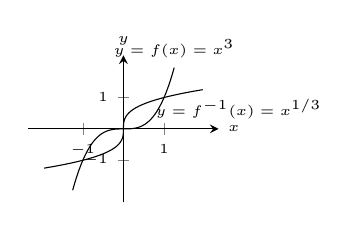
\begin{tikzpicture}[font=\tiny,declare function={f(\x)=\x^3;}]
\begin{axis}[clip=false,width=4cm,axis lines=middle,xlabel={$x$},ylabel={$y$},xlabel style={at={(current axis.right of origin)},anchor=west},ylabel style={at={(current axis.above origin)},anchor=south}, xtick={-1,1},ytick={-1,1}, enlargelimits=true]
\addplot[domain=0:1.25]{f(x)}node[above]{$y=f(x)=x^3$};
\addplot[domain=0:1.25](-x,{-f(x)});
\addplot[domain=0:1.25]({f(x)},x)node[below,xshift=3ex]{$y=f^{-1}(x)=x^{1/3}$};
\addplot[domain=0:1.25]({-f(x)},-x);
\end{axis}
\end{tikzpicture}
\caption{ترسیم جواب \حوالہ{سوال_ماورائی_تصدیق_تفرق_درکار_ت}}
\label{شکل_جواب_ماورائی_تصدیق_تفرق_درکار_ت}
\end{minipage}
\end{figure}
%===================================
\ابتدا{سوال}\شناخت{سوال_ماورائی_تصدیق_تفرق_درکار_ت}
\begin{enumerate}
\item
دکھائیں کہ \عددی{f(x)=x^3} اور \عددی{g(x)=\sqrt[3]{x}} ایک دوسرے کے الٹ ہیں۔
\item
\عددی{f} اور \عددی{g} ترسیم کریں جس میں ان کے نقاط تقاطع \عددی{(1,1)} اور \عددی{(-1,-1)} نظر آئیں۔ آپ کو لکیر \عددی{y=x} میں تشاکلی نظر آنی چاہیے۔
\item
نقاط \عددی{(1,1)} اور \عددی{(-1,-1)} پر \عددی{f} اور \عددی{g} کی ترسیمات کے مماس کی ڈھلوان تلاش کریں۔ (کل چار مماس۔)
\item
مبدا پر ان منحنیات کے مماس تلاش کریں۔
\end{enumerate}
جواب:\quad
(ب) شکل \حوالہ{شکل_جواب_ماورائی_تصدیق_تفرق_درکار_ت}، (ج) \عددی{(1,1)} پر \عددی{f} کی ڈھلوان \عددی{3} ہے؛ \عددی{(1,1)} پر \عددی{g} کی ڈھلوان \عددی{\tfrac{1}{3}} ہے؛ \عددی{-1,-1} پر \عددی{f} کی ڈھلوان \عددی{3} اور \عددی{(-1,-1)} پر \عددی{g} ڈھلوان \عددی{\tfrac{1}{3}} ہے۔  (د) \عددی{x=0} پر \عددی{y=x^3} کا مماس \عددی{y=0} ہے؛ \عددی{x=0} پر \عددی{y=\sqrt[3]{x}} کا مماس \عددی{x=0} ہے۔
\انتہا{سوال}
%========================
\ابتدا{سوال}
\begin{enumerate}
\item
دکھائیں کہ \عددی{h(x)=\tfrac{x^3}{4}} اور \عددی{k(x)=(4x)^{1/3}} ایک دوسرے کے الٹ ہیں۔
\item
\عددی{h} اور \عددی{k} ترسیم کریں جس میں ان کے نقاط تقاطع \عددی{(2,2)} اور \عددی{(-2,-2)} نظر آئیں۔ آپ کو لکیر \عددی{y=x} میں تشاکلی نظر آنی چاہیے۔
\item
نقاط \عددی{(2,2)} اور \عددی{(-2,-2)} پر \عددی{h} اور \عددی{k} کی ترسیمات کے مماس کی ڈھلوان تلاش کریں۔ (کل چار مماس۔)
\item
مبدا پر ان منحنیات کے مماس تلاش کریں۔
\end{enumerate}
\انتہا{سوال}
%========================
\ابتدا{سوال}
مان لیں \عددی{f(x)=x^3-3x^2-1,\,x\ge 2} ہے۔ نقطہ \عددی{x=-1=f(3)} پر \عددی{\tfrac{\dif f^{-1}}{\dif x}} کی قیمت تلاش کریں۔\\
جواب:\quad
$\tfrac{1}{9}$
\انتہا{سوال}
%=======================
\ابتدا{سوال}
مان لیں \عددی{f(x)=x^2-4x-5,\,x> 2} ہے۔ نقطہ \عددی{x=0=f(5)} پر \عددی{\tfrac{\dif f^{-1}}{\dif x}} کی قیمت تلاش کریں۔
\انتہا{سوال}
%=======================
\ابتدا{سوال}
فرض کریں قابل تفرق تفاعل \عددی{y=f(x)} کا الٹ پایا جاتا ہے اور \عددی{f} کی ترسیم نقطہ \عددی{(2,4)} سے گزرتی ہے جہاں اس کی ڈھلوان \عددی{\tfrac{1}{3}} ہے۔ نقطہ \عددی{x=4} پر \عددی{\tfrac{\dif f^{-1}}{\dif x}} کی قیمت تلاش کریں۔\\
جواب:\quad
$3$
\انتہا{سوال}
%=====================
\ابتدا{سوال}
فرض کریں قابل تفرق تفاعل \عددی{y=g(x)} کا الٹ پایا جاتا ہے اور \عددی{g} کی ترسیم مبدا سے گزرتی ہے جہاں اس کی ڈھلوان \عددی{2} ہے۔ مبدا پر \عددی{g^{-1}} کی ترسیم کی ڈھلوان تلاش کریں۔
\انتہا{سوال}
%===================
\ابتدا{سوال}
\begin{enumerate}[a.]
\item
تفاعل \عددی{f(x)=mx} کا الٹ تلاش کریں جہاں \عددی{m} غیر صفر مستقل ہے۔
\item
تفاعل \عددی{y=f(x)} کی ترسیم مبدا سے گزرتی لکیر ہے جس کی ڈھلوان \عددی{m} غیر صفر ہے۔ اس تفاعل کے الٹ کے بارے میں کیا کہا جا سکتا ہے؟
\end{enumerate}
جواب:\quad
(ا) \عددی{f^{-1}(x)=\tfrac{x}{m}}، (ب) \عددی{f^{-1}} کی ترسیم مبدا سے گزرتی ہے اور اس کی ڈھلوان \عددی{\tfrac{1}{m}} ہے۔ 
\انتہا{سوال}
%======================
\ابتدا{سوال}
دکھائیں کہ \عددی{f(x)=mx+b}، جہاں \عددی{m} اور \عددی{b} مستقل ہیں اور \عددی{m\ne 0} ہے، کا الٹ ایک لکیر ہے جس کی
 ڈھلوان \عددی{\tfrac{1}{m}} ہے اور جو محور \عددی{y} کو \عددی{-\tfrac{b}{m}} پر قطع کرتی ہے۔
\انتہا{سوال}
%===================
\ابتدا{سوال}
\begin{enumerate}[a.]
\item
تفاعل \عددی{f(x)=x+1} کا الٹ تلاش کریں۔ \عددی{f} اور اس کا الٹ ایک ساتھ ترسیم کریں۔ لکیر \عددی{y=x} کو بھی شامل کریں۔
\item
تفاعل \عددی{f(x)=x+b}  کا الٹ تلاش کریں جہاں \عددی{b} مستقل ہے۔ \عددی{f^{-1}} کی ترسیم کا \عددی{f} کی ترسیم کے ساتھ کیا تعلق ہے؟
\item
لکیر \عددی{y=x} کے متوازی تفاعل کے الٹ کے بارے میں کیا کہنا ممکن ہو گا؟
\end{enumerate}
جواب:\quad
(ا) \عددی{f^{-1}(x)=x-1}، (ب) \عددی{f^{-1}(x)=x-b}، \عددی{f^{-1}} کی ترسیم \عددی{f} کی ترسیم کے متوازی ہے۔\عددی{f^{-1}} اور \عددی{f} کی ترسیمات لکیر \عددی{y=x} کے مخالف اطراف پر اور اس لکیر سے برابر فاصلہ پر ہیں۔ (ج) ترسیمات ایک دوسرے کے متوازی ہوں گے اور لکیر \عددی{y=x} کے مخالف اطراف اور برابر فاصلہ پر ہوں گے۔
\انتہا{سوال}
%=====================
\ابتدا{سوال}
\begin{enumerate}[a.]
\item
تفاعل \عددی{f(x)=-x+1} کا الٹ معلوم کریں۔ لکیر \عددی{y=-x+1} اور لکیر \عددی{y=x} کو ایک ساتھ ترسیم کریں۔ ان لکیروں کے بیچ زاویہ کتنا ہے۔
\item
تفاعل \عددی{f(x)=-x+b} کا الٹ معلوم کریں جہاں \عددی{b} مستقل ہے۔ لکیر \عددی{y=-x+b} اور لکیر \عددی{y=x} کے مابین زاویہ کتنا ہے؟
\item
لکیر \عددی{y=x} کے عمودی تفاعل کے الٹ کے بارے میں کیا کہا جا سکتا ہے؟
\end{enumerate}
\انتہا{سوال}
%========================
\موٹا{بڑھتا ہوا اور گھٹتا ہوا تفاعل}\\
\ابتدا{سوال}\شناخت{سوال_ماورائی_بڑھتا_گھٹتا_تفاعل}
اگر وقفہ \عددی{I} میں کسی دو نقطوں \عددی{x_1} اور \عددی{x_2} پر 
\begin{align*}
x_2>x_1\quad \implies f(x_2)>f(x_1)
\end{align*}
ہو تب \عددی{I} پر تفاعل \عددی{f(x)} بڑھتا ہو گا (حصہ \حوالہ{حصہ_استعمال_مسئلہ_اوسط_قیمت})۔اسی طرح  درج ذیل صورت میں \عددی{I} پر \عددی{f(x)} گھٹتا ہو گا۔
\begin{align*}
x_2>x_1\quad \implies f(x_2)<f(x_1)
\end{align*}
دکھائیں کہ بڑھتے تفاعل اور گھٹتے تفاعل ایک ایک تفاعل ہیں یعنی دکھائیں کہ \عددی{I} میں کسی بھی دو نقطوں \عددی{x_1} اور \عددی{x_2} کے لئے \عددی{x_2\ne x_1} سے مراد \عددی{f(x_2)\ne f(x_1)} ہو گا۔ 
\انتہا{سوال}
%======================
سوال \حوالہ{سوال_ماورائی_الٹ_پایا_الف} تا سوال \حوالہ{سوال_ماورائی_الٹ_پایا_ب} میں سوال \حوالہ{سوال_ماورائی_بڑھتا_گھٹتا_تفاعل} کے نتائج استعمال کرتے ہوئے دکھائیں کہ دیے تفاعل کا اپنے وقفہ پر الٹ پایا جاتا ہے۔ مسئلہ \حوالہ{مسئلہ_ماورائی_الٹ_تفرق_قاعدہ} کی مدد سے \عددی{\tfrac{\dif f^{-1}}{\dif x}} کا کلیہ تلاش کریں۔

\ابتدا{سوال}\شناخت{سوال_ماورائی_الٹ_پایا_الف}
$f(x)=\tfrac{x}{3}+\tfrac{5}{6}$
\انتہا{سوال}
%============================
\ابتدا{سوال}
$f(x)=27x^3$\\
جواب:\quad
بڑھتا، لہٰذا ایک ایک؛ \عددی{\tfrac{\dif f^{-1}}{\dif x}=\tfrac{1}{9}x^{-2/3}}
\انتہا{سوال}
%============================
\ابتدا{سوال}
$f(x)=1-8x^3$
\انتہا{سوال}
%============================
\ابتدا{سوال}
$f(x)=(1-x)^3$\\
جواب:\quad
گھٹتا، لہٰذا ایک ایک؛ \عددی{\tfrac{\dif f^{-1}}{\dif x}=-\tfrac{1}{3}x^{-2/3}}
\انتہا{سوال}
%============================
\ابتدا{سوال}\شناخت{سوال_ماورائی_الٹ_پایا_ب}
$f(x)=x^{5/3}$
\انتہا{سوال}
%============================
\موٹا{نظریہ اور استعمال}\\
\ابتدا{سوال}
اگر \عددی{f(x)} ایک ایک ہو تب \عددی{g(x)=-f(x)} کے بارے میں کیا کہا جا سکتا ہے؟ اپنے جواب کی وجہ پیش کریں۔
\انتہا{سوال}
%====================
\ابتدا{سوال}
اگر \عددی{} ایک ایک اور غیر صفر ہو تب \عددی{h(x)=\tfrac{1}{f(x)}} کے بارے میں کیا کہنا ممکن ہے؟ اپنے جواب کی وجہ پیش کریں۔
\انتہا{سوال}
%===================
\ابتدا{سوال}
فرض کریں کہ \عددی{g} کی سعت، \عددی{f} کے دائرہ کار میں پائی جاتی ہے لہٰذا مرکب تفاعل \عددی{f\circ g} معین ہے۔ اگر \عددی{f} اور \عددی{g} ایک ایک ہوں تب \عددی{f\circ g} کے بارے میں کیا کہنا ممکن ہو گا؟ اپنے جواب کی وجہ پیش کریں۔
\انتہا{سوال}
%======================
\ابتدا{سوال}
اگر مرکب تفاعل \عددی{f\circ g} ایک ایک ہو تب کیا \عددی{g} لازماً ایک ایک ہو گا؟ اپنے جواب کی وجہ پیش کریں۔
\انتہا{سوال}
%===================
\ابتدا{سوال}
فرض کریں وقفہ \عددی{[a,b]} پر \عددی{f(x)} مثبت، استمراری ور بڑھتا تفاعل  ہے۔ ترسیم کی تاویل کرتے ہوئے درج ذیل دکھائیں۔
\begin{align*}
\int_a^bf(x)\dif x+\int_{f(a)}^{f(b)}f^{-1}\dif x=bf(b)-af(a)
\end{align*}
\انتہا{سوال}
%====================
\ابتدا{سوال}
مستقل \عددی{a}، \عددی{b}، \عددی{c} اور \عددی{d} پر مسلط وہ شرائط تلاش کریں جو ناطق تفاعل
\begin{align*}
f(x)=\frac{ax+b}{cx+d}
\end{align*}
کا الٹ ممکن بناتے ہیں۔
\انتہا{سوال}
%====================
\ابتدا{سوال}
اگر ہم \عددی{f^{-1}(x)} کی جگہ \عددی{g(x)} لکھیں تب مساوات \حوالہ{مساوات_ماورائی_قاعدہ_الٹ_تفرق_الف} کو درج ذیل لکھا جا سکتا ہے۔
\begin{align*}
g'(f(a))=\frac{1}{f'(a)}\quad \implies g'(f(a))\cdot f'(a)=1
\end{align*}
اس میں \عددی{a} کی جگہ \عددی{x} پر کرنے سے  
\begin{align*}
g'(f(x))\cdot f'(x)=1
\end{align*}
ملتا ہے جو زنجیری قاعدہ یاد دلاتی ہے۔ یقیناً درج بالا اور زنجیری قاعدے کے بیچ تعلق پایا جاتا ہے۔

فرض کریں \عددی{f} اور \عددی{g} قابل تفرق اور ایک دوسرے کے الٹ ہیں لہٰذا \عددی{(f\circ g)(x)=x} ہو گا۔ زنجیری قاعدہ استعمال کرتے ہوئے اس مساوات کے دونوں اطراف کا \عددی{x} کے لحاظ سے  تفرق لے کر  \عددی{(f\circ g)'(x)} کو \عددی{f} اور \عددی{g} کے تفرق کی صورت میں لکھ کر دیکھیں  کیا حاصل ہوتا ہے؟ (مسئلہ \حوالہ{مسئلہ_ماورائی_الٹ_تفرق_قاعدہ} کو دیکھنے کا یہ بھی ایک طریقہ ہے۔)
\انتہا{سوال}
%=========================
\ابتدا{سوال}\ترچھا{ترکیب چھلا اور ترکیب خول کی مساوات}\\
فرض کریں وقفہ \عددی{a\le x\le b} پر \عددی{f} قابل تفرق ہے جہاں \عددی{a>0} ہے اور \عددی{f} کا قابل تفرق الٹ \عددی{f^{-1}} پایا جاتا ہے۔ تفاعل \عددی{f}،  لکیر \عددی{x=a} اور لکیر \عددی{y=f(b)} کے بیچ خطہ کو محور \عددی{y} کے گرد گھما کر جسم طواف پیدا کیا جاتا ہے۔ ترکیب چھلا اور ترکیب خول اس جسم کے حجم  کے کلیات ایک جیسا نتیجہ دیتی ہیں:
\begin{align*}
\int_{f(a)}^{f(b)}\big((f^{-1}(y))^2-a^2\big)\dif y=\int_a^b2\pi x(f(b)-f(x))\dif x
\end{align*}
اس مساوات کو ثابت کرنے کی خاطر درج ذیل متعارف کریں۔
\begin{align*}
C(t)&=\int_{f(a)}^{f(t)}\pi\big((f^{-1}(y))^2-a^2\big)\dif y\\
K(t)&=\int_a^t2\pi x(f(t)-f(x))\dif x
\end{align*}
اس کے بعد دکھائیں کہ \عددی{[a,b]} کے کسی نقطہ پر \عددی{C(t)} اور \عددی{K(t)} کی قیمتیں ایک جیسی ہیں اور \عددی{[a,b]} پر ان کے تفرق بھی ایک جیسے ہیں۔ صفحہ \حوالہصفحہ{سوال_تکمل_یکتائی_حل_کی_شرط} پر سوال \حوالہ{سوال_تکمل_یکتائی_حل_کی_شرط} کے نتیجہ کے  مطابق \عددی{[a,b]} میں تمام \عددی{t} کے لئے \عددی{C(t)=K(t)} ہو گا۔ بالخصوص \عددی{C(b)=K(b)} ہو گا۔
\انتہا{سوال}
%========================
\موٹا{کمپیوٹر کا استعمال}\\
سوال \حوالہ{سوال_ماورائی_کمپیوٹر_تخمینی_تفاعل_الف} تا سوال \حوالہ{سوال_ماورائی_کمپیوٹر_تخمینی_تفاعل_ب} میں آپ چند تفاعل اور ان کے الٹ پر غور کریں گے۔ اس کے علاوہ دیے گئے نقطہ پر ان کے تفرق اور خطی تخمینی تفاعل غور کریں گے۔ ان سوالات میں درج ذیل اقدام کریں۔ 
\begin{enumerate}[a.]
\item
دیے گئے وقفہ پر تفاعل \عددی{y=f(x)} اور اس کا تفرق ترسیم کریں۔ بتلائیں کہ آپ کیسے جانتے ہیں کہ اس وقفہ پر \عددی{f} ایک ایک ہے۔
\item
مساوات \عددی{y=f(x)} کو \عددی{x} کے لئے حل کر کے حاصل الٹ تفاعل کو \عددی{g} سے ظاہر کریں۔
\item
دیے گئے نقطہ \عددی{(x_0,f(x_0))} پر \عددی{f} کے مماس کی مساوات دریافت کریں۔
\item
لکیر \عددی{y=x} کے دوسری جانب تشاکلی نقطہ \عددی{(f(x_0),x_0)} پر \عددی{g} کے مماس کی مساوات دریافت کریں۔ مسئلہ \حوالہ{مسئلہ_ماورائی_الٹ_تفرق_قاعدہ} کی مدد سے اس مماسی لکیر کی ڈھلوان معلوم کریں۔
\item
تفاعل \عددی{f}، \عددی{g}، لکیر \عددی{y=x}، دونوں مماسی خط اور نقطہ \عددی{(x_0,f(x_0))} اور \عددی{(f(x_0),x_0)} کو جوڑنے والا سیدھا خط ترسیم کریں۔ آپ کو جو تشاکلی نظر آتی ہے اس پر تبصرہ کریں؟
\end{enumerate}
\ابتدا{سوال}\شناخت{سوال_ماورائی_کمپیوٹر_تخمینی_تفاعل_الف}
   $y=\sqrt{3x-2},\quad\tfrac{2}{3}\le x\le 4,\quad x_0=3$
\انتہا{سوال}
%===========================
\ابتدا{سوال}
$y=\frac{3x+2}{2x-11},\quad -2\le x\le 2,\quad x_0=\frac{1}{2}$
\انتہا{سوال}
%===========================
\ابتدا{سوال}
$y=\frac{4x}{x^2+1},\quad -1\le x\le 1,\quad x_0=\frac{1}{2}$
\انتہا{سوال}
%===========================
\ابتدا{سوال}
$y=\frac{x^3}{x^2+1},\quad -1\le x\le 1,\quad x_0=\frac{1}{2}$
\انتہا{سوال}
%===========================
\ابتدا{سوال}
$y=x^3-3x^2-1,\quad 2\le x\le 5,\quad x_0=\frac{27}{10}$
\انتہا{سوال}
%===========================
\ابتدا{سوال}
$y=2-x-x^3,\quad -2\le x\le 2,\quad x_0=\frac{3}{2}$
\انتہا{سوال}
%===========================
\ابتدا{سوال}
$y=e^x,\quad -3\le x\le 5,\quad x_0=1$
\انتہا{سوال}
%===========================
\ابتدا{سوال}\شناخت{سوال_ماورائی_کمپیوٹر_تخمینی_تفاعل_ب}
$y=\sin x,\quad -\frac{\pi}{2}\le x\le \frac{\pi}{2},\quad x_0=1$
\انتہا{سوال}
%===========================
سوال \حوالہ{سوال_ماورائی_خفی_حل_الف} اور سوال \حوالہ{سوال_ماورائی_خفی_حل_ب} میں درج بالا تمام اقدام بروئے کار لاتے ہوئے دیے گئے وقفہ پر خفی تفاعل تفاعل کو حل کر کے  \عددی{y=f(x)} اور \عددی{x=f^{-1}(y)} حاصل کریں۔

\ابتدا{سوال}\شناخت{سوال_ماورائی_خفی_حل_الف}
$y^{1/3}-1=(x+2)^3,\quad -5\le x\le 5,\quad x_0=-\frac{3}{2}$
\انتہا{سوال}
%==================
\ابتدا{سوال}\شناخت{سوال_ماورائی_خفی_حل_ب}
$\cos y=x^{1/5},\quad 0\le x\le 1,\quad x_0=\frac{1}{2}$
\انتہا{سوال}
%==================

\حصہ{قدرتی لوگارتھم}
علم حساب اور سائنس میں اہم ترین تفاعل اور الٹ کی جوڑی قدرتی لوگارتھم \عددی{\ln x}اور قوت نما تفاعل \عددی{e^x} کی جوڑی ہے۔ تفاعل \عددی{e^x} کی وضاحت  \عددی{\ln x} سے ہوتی ہے لہٰذا ہم پہلے \عددی{\ln x}  متعارف کرتے ہیں۔لوگارتھم نے پہلے علم حساب میں بہتری پیدا کی۔ لوگارتھم کی  خوبیوں نے سترھویں صدی میں آفاقی میکانیات کا حساب اور ساحل سے دور راہ تلاش کرنا ممکن بنایا۔ اگرچہ آج کل پیچیدہ حساب کمپیوٹر کی مدد سے کیا جاتا ہے، بہر حال لوگارتھم کی خوبیاں آج بھی اتنی ہی اہمیت رکھتی ہیں۔

\جزوحصہء{قدرتی لوگارتھمی تفاعل}
مثبت عدد \عددی{x} کے قدرتی لوگارتھم  کو \عددی{\ln x} لکھا جاتا ہے جس کی تعریف  درج ذیل تکمل دیتا ہے۔
\begin{align*}
\ln x&=\int_1^t \frac{1}{x}\dif t,\quad x>0&&\text{\RL{قدرتی لوگارتھمی تفاعل کی تعریف}}
\end{align*}

اگر \عددی{x>1} ہو تب \عددی{t=1} سے \عددی{t=x} تک منحنی \عددی{y=\tfrac{1}{t}} کے نیچے رقبہ \عددی{\ln x} ہو گا (شکل \حوالہ{شکل_ماورائی_قدرتی_لوگارتھمی_تفاعل_تعریف})۔ اگر \عددی{0<x<1}ہو تب \عددی{x} سے \عددی{1} تک منحنی \عددی{y=\tfrac{1}{t}}  کے نیچے رقبے کا منفی \عددی{\ln x} ہو گا۔ قدرتی لوگارتھمی تفاعل وقفہ \عددی{x\le 0} کے لئے غیر معین ہے۔ لوگارتھمی تفاعل کی تعریف سے درج ذیل ملتا ہے۔
\begin{align*}
\ln 1&=\int_1^1\frac{1}{t}\dif t=0&&\text{\RL{بالائی اور زیریں حد ایک جیسے ہیں}}
\end{align*}
%
\begin{figure}
\centering
\begin{subfigure}{0.45\textwidth}
\centering
\begin{tikzpicture}[font=\small,declare function={f(\x)=ln(\x);g(\x)=1/\x;}]
\begin{axis}[clip=false,small,axis lines=middle,xlabel={$x$},ylabel={$y$},xlabel style={at={(current axis.right of origin)},anchor=west},ylabel style={at={(current axis.above origin)},anchor=south},xmin=0,xtick={1,3},xticklabels={$1$,$x$},ytick={1}]
\addplot[name path=curR,domain=1:3,smooth]{g(x)};;
\addplot[name path=axisR]plot coordinates {(1,0) (3,0)};
\addplot[lgray]fill between[of=curR and axisR];
\addplot[domain=0.3:4,smooth]{g(x)}node[pos=0,right]{$y=\frac{1}{x}$};
\addplot[domain=0.3:4,smooth]{f(x)}node[above left]{$y=\ln x$};
\draw(1,{g(1)})--(1,0)  (3,{g(3)})--(3,0);
\draw(1.2,{g(1.5)})--(1.5,1.5)node[above,align=right]{\RL{$x>1$ کی صورت میں}\\  $\ln x=\int_1^x\tfrac{1}{t}\dif t$};
\draw(1.1,-0.1)--(2,-1)node[below,align=center]{\RL{اگر $x=1$ ہو تب}\\  $\ln 1=\int_1^1\tfrac{1}{t}\dif t=0$};
\end{axis}
\end{tikzpicture}
\end{subfigure}\hfill
\begin{subfigure}{0.45\textwidth}
\centering
\begin{tikzpicture}[font=\small,declare function={f(\x)=ln(\x);g(\x)=1/\x;}]
\begin{axis}[clip=false,small,axis lines=middle,xlabel={$x$},ylabel={$y$},xlabel style={at={(current axis.right of origin)},anchor=west},ylabel style={at={(current axis.above origin)},anchor=south},xmin=0,xtick={0.5,1},xticklabels={$x$,$1$},ytick={1}]
\addplot[name path=curL,domain=0.5:1,smooth]{g(x)};
\addplot[name path=axisL]plot coordinates {(0.5,0) (1,0)};
\addplot[lgray]fill between[of=curL and axisL];
\addplot[domain=0.3:4,smooth]{g(x)}node[pos=0,right]{$y=\frac{1}{x}$};
\addplot[domain=0.3:4,smooth]{f(x)}node[pos=0.8,above]{$y=\ln x$};
\draw(0.5,{g(0.5)})--(0.5,0)  (1,{g(1)})--(1,0);
\draw(0.75,1)--(1.75,1.75)node[above,align=right]{\RL{$x<1$ کی صورت میں}\\  $\ln x=-\int_1^x\tfrac{1}{t}\dif t$};
\draw(1.1,-0.1)--(2,-1)node[below,align=center]{\RL{اگر $x=1$ ہو تب}\\  $\ln 1=\int_1^1\tfrac{1}{t}\dif t=0$};
\end{axis}
\end{tikzpicture}
\end{subfigure}
\caption{
تفاعل \عددی{y=\tfrac{1}{x},\,x>0} اور قدرتی لوگارتھمی تفاعل \عددی{y=\ln x} کا تعلق۔ قدرتی لوگارتھمی تفاعل \عددی{x>1} کے لئے مثبت اور \عددی{x<1} کے لئے منفی ہے۔ 
}
\label{شکل_ماورائی_قدرتی_لوگارتھمی_تفاعل_تعریف}
\end{figure}

دھیان رہے کہ ہم شکل \حوالہ{شکل_ماورائی_قدرتی_لوگارتھمی_تفاعل_تعریف} میں \عددی{y=\tfrac{1}{x}} ترسیم کرتے ہیں لیکن تکمل میں \عددی{y=\tfrac{1}{t}} استعمال کرتے ہیں۔ ہر متغیر کو \عددی{x} لکھنے سے
\begin{align*}
\ln x=\int_1^x\frac{1}{x}\dif x
\end{align*}
لکھا جائے گا جہاں  \عددی{x} کے دو مختلف معنی ہیں۔ اسی لئے ہم تکمل میں متغیر کو تبدیل کرتے ہوئے \عددی{t} لکھتے ہیں۔

\عددی{x} کی مختلف قیمتوں کے لئے  تین اعشاریہ درست قدرتی لوگارتھمی قیمتیں درج ذیل ہیں۔
\begin{align*}
\begin{array}{c|cccccccc}
x&0&0.05&0.5&1&2&3&4&10\\
\hline
\ln x&\text{\RL{غیر معین}} & -3.00&-0.69&0&0.69&1.10&1.39&2.30  
\end{array}
\end{align*}

\جزوحصہء{قدرتی لوگارتھمی تفاعل کا تفرق}
احصاء کے بنیادی مسئلہ کے جزو اول (مسئلہ \حوالہ{مسئلہ_تکمل_بنیادی_مسئلہ_جزو_اول}) سے
\begin{align*}
\frac{\dif}{\dif x}\ln x=\frac{\dif}{\dif x}\int_1^x\frac{1}{t}\dif t=\frac{1}{x}
\end{align*}
لکھا جا سکتا ہے لہٰذا \عددی{x} کی ہر مثبت قیمت کے کئے درج ذیل ہو گا۔
\begin{align*}
\frac{\dif}{\dif x}\ln x=\frac{1}{x}
\end{align*}

اگر \عددی{u} متغیر \عددی{x} کا قابل تفرق تفاعل ہو اور \عددی{u} کی قیمتیں مثبت ہوں، تا کہ \عددی{\ln u} معین  ہو، تب تفاعل \عددی{y=\ln u} پر زنجیری قاعدہ
\begin{align*}
\frac{\dif y}{\dif x}=\frac{\dif y}{\dif u}\frac{\dif u}{\dif x}
\end{align*}
 کی اطلاق سے 
\begin{align*}
\frac{\dif}{\dif x}\ln u=\frac{\dif}{\dif u}\ln u\cdot \frac{\dif u}{\dif x}=\frac{1}{u}\frac{\dif u}{\dif x}
\end{align*}
ملتا ہے لہٰذا درج ذیل ہو گا۔
\begin{align}\label{مساوات_ماورائی_لوگارتھمی_تفرق_الف}
\frac{\dif}{\dif x}\ln u=\frac{1}{u}\frac{\dif u}{\dif x},\quad u>0
\end{align}

\ابتدا{مثال}\شناخت{مثال_ماورائی_قدرتی_لوگارتھمی_تفرق}
\begin{align*}
\frac{\dif}{\dif x}\ln 2x=\frac{1}{2x}\frac{\dif}{\dif x}(2x)=\frac{1}{2x}(2)=\frac{1}{x}
\end{align*}
\انتہا{مثال}
%=====================

آپ نے مثال \حوالہ{مثال_ماورائی_قدرتی_لوگارتھمی_تفرق} میں دیکھا کہ تفاعل \عددی{y=\ln 2x} کا تفرق وہی ہے جو تفاعل \عددی{y=\ln x} کا ہے۔ درحقیقت کسی بھی تفاعل \عددی{y=\ln ax} کے لئے درست ہے جہاں \عددی{a} کوئی عدد ہے:
\begin{align}\label{مساوات_ماورائی_لوگارتھمی_تفرق_ب}
\frac{\dif}{\dif x}\ln ax=\frac{1}{ax}\frac{\dif}{\dif x}(ax)=\frac{1}{ax}(ax)=\frac{1}{x}
\end{align}

\ابتدا{مثال}
اگر مساوات \حوالہ{مساوات_ماورائی_لوگارتھمی_تفرق_الف} میں \عددی{u=x^2+3} پر کیا جائے تب درج ذیل ہو گا۔
\begin{align*}
\frac{\dif}{\dif x}\ln(x^2+3)=\frac{1}{x^2+3}\cdot\frac{\dif}{\dif x}(x^2+3)=\frac{1}{x^2+3}\cdot 2x=\frac{2x}{x^2+3}
\end{align*}
\انتہا{مثال}
%=====================

\جزوحصہء{خواص لوگارتھم}
کمپیوٹر کی ایجاد سے پہلے  علم حساب میں سب سے زیادہ بہتری  لوگارتھم کے سر ہے\حاشیہد{اسکاچی ریاضی دان جان نیپر نے سولہویں صدی میں لوگارتھم ایجاد کیا۔ انہوں نے اپنی زندگی کے آخری بیس برس لوگارتھمی جدول مکمل کرنے میں صرف کیے}۔ لوگارتھم کی وہ خوبیاں جن کی بدولت حساب میں بہتری پیدا ہوئی جدول \حوالہ{جدول_ماورائی_خواص_قدرتی_لوگارتھم} میں دی گئی ہیں۔ ان خواص کی بنا مثبت اعداد کے ضرب کی جگہ جمع اور مثبت اعداد کی تقسیم کی جگہ تفریق استعمال ہونے لگا۔ اس کے علاوہ طاقت کی جگہ ضرب استعمال کیا جانے لگا۔ وقتی طور پر ہم جزو د میں طاقت \عددی{n} کو ناطق عدد تصور کرتے ہیں۔ اس کی وضاحت جزو د کے ثبوت کے دوران ہو گی۔  
\begin{table}
\caption{خواص قدرتی لوگارتھم}
\label{جدول_ماورائی_خواص_قدرتی_لوگارتھم}
\centering
\begin{tabular}{crl}
 \toprule
\multicolumn{3}{c}{\RL{کسی بھی اعداد \عددی{a>0} اور \عددی{x>0} کے لئے۔}}\\
\midrule
الف& قاعدہ ضرب& $\ln ax=\ln a+\ln x$\\
ب&قاعدہ حاصل تقسیم & $\ln \frac{a}{x}=\ln a-\ln x$\\
ج&قاعدہ بالعکس متناسب& $\ln \frac{1}{x}=-\ln x$\\
د&قاعدہ طاقت&$\ln x^n=n\ln x$\\
\bottomrule
\end{tabular}
\end{table}

\ابتدا{مثال}
\begin{align*}
\ln 6&=\ln (2\cdot 3)=\ln 2+\ln 3&&\text{\RL{ضرب}}\\
\ln 4-\ln 5&=\ln \frac{4}{5}=\ln 0.8&&\text{\RL{حاصل تقسیم}}\\
\ln \frac{1}{8}&=-\ln 8&&\text{\RL{بالعکس متناسب}}\\
&=-\ln 2^3=-3\ln 2&&\text{\RL{طاقت}}
\end{align*}
\انتہا{مثال}
%====================
\ابتدا{مثال}
\begin{align*}
\ln 4+\ln\sin x&=\ln (4\sin x)&&\text{\RL{ضرب}}\\
\ln\frac{x+1}{2x-3}&=\ln(x+1)-\ln(2x-3)&&\text{\RL{حاصل تقسیم}}\\
\ln \sec x&=\ln \frac{1}{\cos x}=-\ln \cos x&&\text{\RL{بالعکس متناسب}}\\
\ln\sqrt[3]{x+1}&=\ln(x+1)^{1/3}=\frac{1}{3}\ln(x+1)&&\text{\RL{طاقت}}
\end{align*}
\انتہا{مثال}
%====================

\ابتدا{ثبوت}\موٹا{برائے $\ln ax=\ln a+\ln x$}\\
اس کا دلیل عجیب اور  عمدہ ہے۔ ہم دیکھتے ہیں کہ \عددی{\ln ax} کا تفرق اور \عددی{\ln x} کا تفرق ایک دوسرے کے برابر ہیں (مساوات \حوالہ{مساوات_ماورائی_لوگارتھمی_تفرق_ب})۔ مسئلہ اوسط قیمت کے ضمنی نتیجہ دوم (صفحہ \حوالہ{نتیجہ_صریح_استعمال_دوم}) کہتا ہے کہ ان تفاعل میں مستقل کا فرق ہو گا:
\begin{align}\label{مساوات_ماورائی_مستقل_کیا_الف}
\ln ax&=\ln x+C &&\text{\RL{$C$ مستقل}}
\end{align}
اب صرف یہ دکھانا باقی ہے کہ \عددی{C} اور \عددی{\ln a} ایک دوسرے کے برابر ہیں۔

مساوات \حوالہ{مساوات_ماورائی_مستقل_کیا_الف} \عددی{x} کی تمام مثبت قیمتوں کے لئے درست ہے لہٰذا یہ \عددی{x=1} کے لئے بھی درست ہو گا۔یوں درج ذیل ہو گا۔
\begin{align*}
\ln (a\cdot 1)&=\ln 1+C\\
\ln a&=0+C&&\ln 1=0\\
C&=\ln a&&\text{\RL{ترتیب دی گئی ہے}}
\end{align*}
مساوات \حوالہ{مساوات_ماورائی_مستقل_کیا_الف} میں \عددی{C=\ln a} پر کرنے سے ہمیں درکار تعلق حاصل ہوتا ہے۔
\begin{align}\label{مساوات_ماورائی_مستقل_کیا_ب}
\ln ax=\ln a+\ln x
\end{align}
\انتہا{ثبوت}
%====================

\ابتدا{ثبوت}\موٹا{برائے $\ln\tfrac{a}{x}=\ln a-\ln x$}\\
ہم مساوات \حوالہ{مساوات_ماورائی_مستقل_کیا_ب} کو دو بار استعمال کر کے ثبوت پیش کرتے ہیں۔ مساوات \حوالہ{مساوات_ماورائی_مستقل_کیا_ب} میں \عددی{a} کی جگہ \عددی{\tfrac{1}{x}} پر کرنے سے
\begin{align*}
\ln\frac{1}{x}+\ln x&=\ln \big(\frac{1}{x}\cdot x\big)\\
&=\ln 1=0
\end{align*}
ملتا ہے لہٰذا 
\begin{align*}
\ln\frac{1}{x}=-\ln x
\end{align*}
ہو گا۔ مساوات \حوالہ{مساوات_ماورائی_مستقل_کیا_ب} میں \عددی{x} کی جگہ \عددی{\tfrac{1}{x}} پر کرنے سے
\begin{align*}
\ln\frac{a}{x}&=\ln\big(a\cdot \frac{1}{x}\big)=\ln a+\ln \frac{1}{x}\\
&=\ln a-\ln x
\end{align*}
ملتا ہے۔
\انتہا{ثبوت}
%=====================

\ابتدا{ثبوت}\موٹا{برائے $\ln x^n=n\ln x$ جہاں \عددی{n} ناطق ہے}\\
تمام مثبت \عددی{x} قیمتوں کے لئے درج ذیل ہو گا۔ (درج ذیل میں یاد رہے کہ ہم نے طاقتی قاعدہ صرف ناطق اعداد کے لئے ثابت کیا ہے۔)
\begin{align*}
\frac{\dif}{\dif x}\ln x^n&=\frac{1}{x^n}\frac{\dif}{\dif x}(x^n)&&\text{\RL{مساوات \حوالہ{مساوات_ماورائی_لوگارتھمی_تفرق_الف} میں $u=x^n$}}\\
&=\frac{1}{x^n}nx^{n-1}&&\text{\RL{یہاں $n$ کا ناطق ہونا ضروری ہے}}\\
&=n\cdot \frac{1}{x}=\frac{\dif}{\dif x}(n\ln x)
\end{align*}
چونکہ \عددی{\ln x^n} اور \عددی{n\ln x} کے تفرق ایک دوسرے کے برابر ہیں لہٰذا
\begin{align*}
\ln x^n&=n\ln x+C&&\text{\RL{$C$ مستقل}}
\end{align*}
ہو گا جس میں \عددی{x=1} پر کرنے سے \عددی{C=0} ملتا ہے۔
\انتہا{ثبوت}
%=================

اگرچہ ہم نے غیر ناطق \عددی{n} کے لئے قاعدہ \عددی{\ln x^n=n\ln x} ثابت نہیں کیا ہے، یہ قاعدہ غیر ناطق اعداد کے لئے بھی درست ہے لہٰذا اس کو بغیر فقر استعمال کریں۔ 

\جزوحصہء{$\ln x$ کی ترسیم اور سعت}
چونکہ \عددی{x>0} کے لئے  \عددی{\tfrac{\dif}{\dif x}(\ln x)=\tfrac{1}{x}} ہے لہٰذا \عددی{\ln x} متغیر \عددی{x} کا بڑھتا تفاعل ہے۔ اس کا دو رتبی تفرق، \عددی{-\tfrac{1}{x^2}}، منفی ہے لہٰذا \عددی{\ln x} کی ترسیم نیچے مقعر ہے۔

اعدادی تراکیب سے  \عددی{\ln 2} کی قیمت تقریباً \عددی{0.69} حاصل ہوتی ہے۔یوں
\begin{align*}
\ln 2^n=n\ln 2>n\big(\frac{1}{2}\big)=\frac{n}{2}
\end{align*}
اور
\begin{align*}
\ln 2^{-n}=-n\ln 2<-n\big(\frac{1}{2}\big)=-\frac{n}{2}
\end{align*}
ہوں گے۔ان سے درج ذیل اخذ کیے جا سکتے ہیں۔
\begin{align*}
\lim_{x\to \infty}\ln x=\infty\quad \text{اور}\quad \lim_{x\to 0^+}\ln x=-\infty
\end{align*}
\عددی{\ln x} کا دائرہ کار مثبت حقیقی اعداد کا سلسلہ ہے جبکہ \عددی{\ln x} کی سعت پوری حقیقی لکیر ہے۔

\جزوحصہء{لوگارتھمی تفرق}
حاصل ضرب، حاصل تقسیم اور طاقت  پر مبنی مثبت تفاعل کا تفرق لینے سے پہلے  تفاعل کا لوگارتھم لینا سودمند ثابت ہوتا ہے۔ لوگارتھم لیتے ہوئے ہم جدول \حوالہ{جدول_ماورائی_خواص_قدرتی_لوگارتھم} کے قواعد استعمال کرتے ہوئے تفاعل کی سادہ صورت حاصل کرتے ہیں جس کا تفرق نسبتاً آسانی سے حاصل ہوتا ہے۔ اس عمل کو \اصطلاح{لوگارتھمی تفرق}\فرہنگ{لوگارتھمی تفرق}\حاشیہب{logarithmic differentiation}\فرہنگ{differentiation!logarithmic} کہتے ہیں۔ 

\ابتدا{مثال}
تفاعل \عددی{y=\tfrac{(x^2+1)(x+3)^{1/2}}{x-1},\, x>1} کے لئے \عددی{} تلاش کریں۔

حل:\quad
ہم دونوں اطراف کا قدرتی لوگارتھم لے کر جدول \حوالہ{جدول_ماورائی_خواص_قدرتی_لوگارتھم} کے قواعد سے سادہ صورت حاصل کرتے ہیں۔
\begin{align*}
\ln y&=\ln \frac{(x^2+1)(x+3)^{1/2}}{x-1}\\
&=\ln \big((x^2+1)(x+3)^{1/2}\big)-\ln(x-1)&&\text{\RL{قاعدہ حاصل تقسیم}}\\
&=\ln (x^2+1)+\ln (x+3)^{1/2}-\ln(x-1)&&\text{\RL{قاعدہ ضرب}}\\
&=\ln(x^2+1)+\frac{1}{2}\ln (x+3)-\ln(x-1)&&\text{\RL{قاعدہ طاقت}}
\end{align*}
اب ہم دونوں اطراف کا \عددی{x} کے لحاظ سے تفرق لیتے ہیں۔ (بائیں ہاتھ مساوات \حوالہ{مساوات_ماورائی_لوگارتھمی_تفرق_الف} استعمال کرتے ہیں۔)
\begin{align*}
\frac{1}{y}\frac{\dif y}{\dif x}=\frac{1}{x^2+1}\cdot 2x+\frac{1}{2}\cdot\frac{1}{x+3}-\frac{1}{x-1}
\end{align*}
اس کو \عددی{\tfrac{\dif y}{\dif x}} کے لئے حل کرتے ہیں:
\begin{align*}
\frac{\dif y}{\dif x}=y\big(\frac{2x}{x^2+1}+\frac{1}{2x+6}-\frac{1}{x-1}\big)
\end{align*}
آخر میں ہم \عددی{y} کی قیمت پر کرتے ہیں:
\begin{align*}
\frac{\dif y}{\dif x}= \frac{(x^2+1)(x+3)^{1/2}}{x-1}\big(\frac{2x}{x^2+1}+\frac{1}{2x+6}-\frac{1}{x-1}\big)
\end{align*}
\انتہا{مثال}
%======================

\جزوحصہء{تفاعل \عددی{y=f(x)>0} کا لوگارتھمی تفرق}
کسی بھی تفاعل کا لوگارتھمی تفرق درج ذیل اقدام سے حاصل ہو گا۔
\begin{align*}
\ln y&=\ln f(x)&&\text{\RL{دونوں اطراف لوگارتھم لیں}}\\
\frac{\dif}{\dif x}\ln y&=\frac{\dif}{\dif x}(\ln f(x))&&\text{\RL{دونوں اطراف تفرق لیں}}\\
\frac{1}{y}\frac{\dif y}{\dif x}&=\frac{\dif}{\dif x}(\ln f(x))&&\text{\RL{بائیں ہاتھ مساوات \حوالہ{مساوات_ماورائی_لوگارتھمی_تفرق_الف}}}\\
\frac{\dif y}{\dif x}&=y\frac{\dif}{\dif x}(\ln f(x))&&\text{\RL{$\frac{\dif y}{\dif x}$ کے لئے حل کریں}}\\
\frac{\dif y}{\dif x}&=f(x)\frac{\dif}{\dif x}(\ln f(x))&&\text{\RL{$y=f(x)$ پر کریں}}
\end{align*}

\جزوحصہء{تکمل $\int \tfrac{\dif u}{u}$}
مساوات \حوالہ{مساوات_ماورائی_لوگارتھمی_تفرق_الف} سے تکمل کا کلیہ 
\begin{align}\label{مساوات_ماورائی_تفاعل_لوگارتھمی_تکمل_الف}
\int\frac{1}{u}\dif u&=\ln u+C&&\text{\RL{$C$مستقل}}
\end{align}
ملتا ہے  جہاں \عددی{u} مثبت قابل تفرق تفاعل ہے۔ منفی \عددی{u} کی صورت میں کیا ہو گا؟ اگر \عددی{u} منفی ہو تب \عددی{-u} مثبت ہو گا لہٰذا
\begin{gather}
\begin{aligned}\label{مساوات_ماورائی_تفاعل_لوگارتھمی_تکمل_ب}
\int\frac{1}{u}\dif u&=\int\frac{1}{(-u)}\dif (-u)\\
&=\ln (-u)+C&&\text{\RL{مساوات \حوالہ{مساوات_ماورائی_تفاعل_لوگارتھمی_تکمل_الف} میں \عددی{u} کی جگہ \عددی{-u}}}
\end{aligned}
\end{gather}
لکھا جا سکتا ہے۔ مساوات \حوالہ{مساوات_ماورائی_تفاعل_لوگارتھمی_تکمل_الف} اور مساوات \حوالہ{مساوات_ماورائی_تفاعل_لوگارتھمی_تکمل_ب}  میں دائیں ہاتھ کو \عددی{\ln\abs{x}+C} لکھا جا سکتا ہے۔ یوں دونوں مساوات کو
\begin{align}\label{مساوات_ماورائی_تفاعل_لوگارتھمی_تکمل_پ}
\int\frac{1}{u}\dif u=\ln\abs{u}+C
\end{align}
میں ضم کیا جا سکتا ہے جہاں \عددی{u} غیر صفر قابل تفرق تفاعل ہے۔

ہم درج ذیل جانتے ہیں
\begin{align*}
\int u^n\dif u=\frac{u^{n+1}}{n+1}+C,\quad n\ne -1
\end{align*}
اور \عددی{n=-1} کے لئے مساوات \حوالہ{مساوات_ماورائی_تفاعل_لوگارتھمی_تکمل_پ} کی طرف دیکھ سکتے ہیں۔

مساوات \حوالہ{مساوات_ماورائی_تفاعل_لوگارتھمی_تکمل_پ} کے تحت درج ذیل ہو گا
\begin{align*}
\int\frac{f'(x)}{f(x)}\dif x=\ln\abs{f(x)}+C
\end{align*}
جہاں \عددی{f(x)} قابل تفرق تفاعل ہے جس کی علامت پورے دائرہ کار پر تبدیل نہیں ہوتی ہے۔

\ابتدا{مثال}
\begin{align*}
\int_0^2\frac{2x}{x^2-5}\dif x&=\int_{-5}^{-1}\frac{\dif u}{u}=\left.\ln\abs{u}\right\vert_{-5}^{-1}&&u=x^2-5\\
&=\ln\abs{-1}-\ln\abs{-5}=\ln 1-\ln 5=-\ln 5
\end{align*}
\انتہا{مثال}
%======================
\ابتدا{مثال}
\begin{align*}
\int_{-\pi/2}^{\pi/2}\frac{4\cos \theta}{3+2\sin\theta}\dif \theta&=\int_1^5\frac{2}{u}\dif u&&u=3+2\sin\theta\\
&=\left.2\ln\abs{u}\right\vert_{1}^{5}\\
&=2\ln\abs{5}-2\ln\abs{1}=2\ln 5
\end{align*}
\انتہا{مثال}
%=================

\جزوحصہء{$\tan x$ اور $\cot x$ کے تکمل}
ہمیں مساوات \حوالہ{مساوات_ماورائی_تفاعل_لوگارتھمی_تکمل_پ} کی مدد سے \عددی{\tan x} اور \عددی{\cot x} کا تکمل لے سکتے ہیں۔ٹینجنٹ کے لئے درج ذیل ہو گا۔
\begin{align*}
\int\tan x\dif x&=\int\frac{\sin x}{\cos x}\dif x=\int\frac{-\dif u}{u}&&u=\cos x\\
&=-\int\frac{\dif u}{u}=-\ln \abs{u}+C&&\text{\RL{مساوات \حوالہ{مساوات_ماورائی_تفاعل_لوگارتھمی_تکمل_پ}}}\\
&=-\ln\abs{\cos x}+C=\ln\frac{1}{\abs{\cos x}}+C&&\text{\RL{قاعدہ بالعکس متناسب}}\\
&=\ln\abs{\sec x}+C
\end{align*}
کوٹینجنٹ کے لئے درج ذیل ہو گا۔
\begin{align*}
\int\cot x\dif x&=\int\frac{\cos x}{\sin x}\dif x=\int\frac{\dif u}{u}&&u=\sin x\\
&=\ln\abs{u}+C=\ln\abs{\sin x}+C=-\ln\abs{\csc x}+C
\end{align*}
اس طرح درج ذیل کلیات حاصل ہوتے ہیں۔
\begin{align*}
\int \tan u \dif u&=-\ln \abs{\cos u}+C=\ln\abs{\sec u}+C\\
\int\cot u\dif u&=\ln \abs{\sin u}+C=-\ln\abs{\csc x}+C
\end{align*}

\ابتدا{مثال}
\begin{align*}
\int_0^{\pi/6}\tan 2x\dif x&=\int_0^{\pi/3}\tan u\cdot \frac{\dif u}{2}=\frac{1}{2}\int_0^{\pi/3}\tan u \dif u&&u=2x\\
&=\left.\frac{1}{2}\ln\abs{\sec u}\right\vert_0^{\pi/3}=\frac{1}{2}(\ln 2-\ln 1)=\frac{1}{2}\ln 2
\end{align*}
\انتہا{مثال}
%=====================

\حصہء{سوالات}
\موٹا{لوگارتھم کے خواص}

\ابتدا{سوال}
مندرجہ ذیل کو \عددی{\ln 2} اور \عددی{\ln 3} کی صورت میں لکھیں۔
\begin{multicols}{3}
\begin{enumerate}[a.]
\item
$\ln 0.75$
\item
$\ln (4/9)$
\item
$\ln (1/2)$
\item
$\ln\sqrt[3]{9}$
\item
$\ln 3\sqrt{2}$
\item
$\ln\sqrt{13.5}$
\end{enumerate}
\end{multicols}
جواب:\quad
(ا) \عددی{\ln 3-2\ln 2}، (ب) \عددی{2(\ln 2-\ln 3)}، (ج) \عددی{-\ln 2}، (د) \عددی{\tfrac{2}{3}\ln 3}، (ہ) \عددی{\ln 3+\tfrac{1}{2}\ln 2}، (و) \عددی{\tfrac{1}{2}(3\ln 3-\ln 2)}
\انتہا{سوال}
%==================
\ابتدا{سوال}
مندرجہ ذیل کو \عددی{\ln 5} اور \عددی{\ln 7} کی صورت میں لکھیں۔
\begin{multicols}{3}
\begin{enumerate}[a.]
\item
$\ln (1/125)$
\item
$\ln 9.8$
\item
$\ln 7\sqrt{7}$
\item
$\ln1225$
\item
$\ln 0.056$
\item
$ \tfrac{\ln 35+\ln(1/7)}{\ln 25}$
\end{enumerate}
\end{multicols}
\انتہا{سوال}
%==================
سوال \حوالہ{سوال_ماورائی_سادہ_الف} اور سوال \حوالہ{سوال_ماورائی_سادہ_ب} میں خواص لوگارتھم کی مدد سے دیے گئے ریاضی فقرے کی سادہ صورت تلاش کریں۔

\ابتدا{سوال}\شناخت{سوال_ماورائی_سادہ_الف}
\begin{multicols}{3}
\begin{enumerate}[a.]
\item
$\ln \sin\theta-\ln \big(\frac{\sin\theta}{5}\big)$
\item
$\ln(3x^2-9x)+\ln\big(\frac{1}{3x}\big)$
\item
$\frac{1}{2}\ln(4t^4)-\ln 2$
\end{enumerate}
\end{multicols}
جواب:\quad
(ا) \عددی{\ln 5}، (ب) \عددی{\ln(x-3)}، (ج) \عددی{\ln(t^2)}
\انتہا{سوال}
%=============================
\ابتدا{سوال}\شناخت{سوال_ماورائی_سادہ_ب}
\begin{multicols}{2}
\begin{enumerate}[a.]
\item
$\ln \sec\theta+\ln\cos\theta$
\item
$\ln(8x+4)-2\ln2$
\item
$3\ln\sqrt[3]{t^2-1}-\ln(t+1)$
\end{enumerate}
\end{multicols}
\انتہا{سوال}
%========================
\موٹا{لوگارتھم کے تفرق}\\
سوال \حوالہ{سوال_ماورائی_لوگارتھم_تفرق_لیں_الف} تا سوال \حوالہ{سوال_ماورائی_لوگارتھم_تفرق_لیں_ب} میں \عددی{x}، \عددی{t} یا \عددی{\theta} کے لحاظ سے \عددی{y} کا تفرق لیں۔

\ابتدا{سوال}\شناخت{سوال_ماورائی_لوگارتھم_تفرق_لیں_الف}
$y=\ln 3x$\\
جواب:\quad
$\tfrac{1}{x}$
\انتہا{سوال}
%====================
\ابتدا{سوال}
$y=\ln kx,\quad \text{\RL{$k$ مستقل}}$
\انتہا{سوال}
%====================
\ابتدا{سوال}
$y=\ln(t^2)$\\
جواب:\quad
$\tfrac{2}{t}$
\انتہا{سوال}
%====================
\ابتدا{سوال}
$y=\ln(t^{3/2})$
\انتہا{سوال}
%====================
\ابتدا{سوال}
$y=\ln\frac{3}{x}$\\
جواب:\quad
$-\tfrac{1}{x}$
\انتہا{سوال}
%====================
\ابتدا{سوال}
$y=\ln\frac{10}{x}$
\انتہا{سوال}
%====================
\ابتدا{سوال}
$y=\ln(\theta+1)$\\
جواب:\quad
$\tfrac{1}{\theta+1}$
\انتہا{سوال}
%====================
\ابتدا{سوال}
$y=\ln(2\theta+2)$
\انتہا{سوال}
%====================
\ابتدا{سوال}
$y=\ln x^3$\\
جواب:\quad
$\tfrac{3}{x}$
\انتہا{سوال}
%====================
\ابتدا{سوال}
$y=(\ln x)^3$
\انتہا{سوال}
%====================
\ابتدا{سوال}
$y=t(\ln t)^2$\\
جواب:\quad
$2\ln t+(\ln t)^2$
\انتہا{سوال}
%====================
\ابتدا{سوال}
$y=t\sqrt{\ln t}$
\انتہا{سوال}
%====================
\ابتدا{سوال}
$y=\frac{x^4}{4}\ln x-\frac{x^4}{16}$\\
جواب:\quad
$x^3\ln x$
\انتہا{سوال}
%====================
\ابتدا{سوال}
$y=\frac{x^3}{3}\ln x-\frac{x^3}{9}$
\انتہا{سوال}
%====================
\ابتدا{سوال}
$y=\frac{\ln t}{t}$\\
جواب:\quad
$\tfrac{1-\ln t}{t^2}$
\انتہا{سوال}
%====================
\ابتدا{سوال}
$y=\frac{1+\ln t}{t}$
\انتہا{سوال}
%====================
\ابتدا{سوال}
$y=\frac{\ln x}{1+\ln x}$\\
جواب:\quad
$\tfrac{1}{x(1+\ln x)^2}$
\انتہا{سوال}
%====================
\ابتدا{سوال}
$y=\frac{x\ln x}{1+\ln x}$
\انتہا{سوال}
%====================
\ابتدا{سوال}
$y=\ln(\ln x)$\\
جواب:\quad
$\tfrac{1}{x\ln x}$
\انتہا{سوال}
%====================
\ابتدا{سوال}
$y=\ln(\ln(\ln x))$
\انتہا{سوال}
%====================
\ابتدا{سوال}
$y=\theta(\sin(\ln \theta))+\cos(\ln \theta)$\\
جواب:\quad
$2\cos (\ln \theta)$
\انتہا{سوال}
%====================
\ابتدا{سوال}
$y=\ln(\sec\theta+\tan\theta)$
\انتہا{سوال}
%====================
\ابتدا{سوال}
$y=\ln\frac{1}{x\sqrt{x+1}}$\\
جواب:\quad
$-\tfrac{3x+2}{2x(x+1)}$
\انتہا{سوال}
%====================
\ابتدا{سوال}
$y=\frac{1}{2}\ln\frac{1+x}{1-x}$
\انتہا{سوال}
%====================
\ابتدا{سوال}
$y=\frac{1+\ln t}{1-\ln t}$\\
جواب:\quad
$\tfrac{2}{t(1-\ln t)^2}$
\انتہا{سوال}
%====================
\ابتدا{سوال}
$y=\sqrt{\ln\sqrt{t}}$
\انتہا{سوال}
%====================
\ابتدا{سوال}
$y=\ln(\sec(\ln\theta))$\\
جواب:\quad
$\tfrac{\tan(\ln\theta)}{\theta}$
\انتہا{سوال}
%====================
\ابتدا{سوال}
$y=\ln\big(\frac{\sqrt{\sin\theta\cos\theta}}{1+2\ln\theta}\big)$
\انتہا{سوال}
%====================
\ابتدا{سوال}
$y=\ln\big(\frac{(x^2+1)^5}{\sqrt{1-x}}\big)$\\
جواب:\quad
$\tfrac{10x}{x^2+1}+\tfrac{1}{2(1-x)}$
\انتہا{سوال}
%====================
\ابتدا{سوال}
$y=\ln\sqrt{\frac{(x+1)^5}{(x+2)^{20}}}$
\انتہا{سوال}
%====================
\ابتدا{سوال}
$y=\int_{x^2/2}^{x^2}\ln\sqrt{t}\dif t$\\
جواب:\quad
$2x\ln\abs{x}-x\ln\tfrac{\abs{x}}{\sqrt{2}}$
\انتہا{سوال}
%====================
\ابتدا{سوال}\شناخت{سوال_ماورائی_لوگارتھم_تفرق_لیں_ب}
$y=\int_{\sqrt{x}}^{\sqrt[3]{x}}\ln t\dif t$
\انتہا{سوال}
%====================

\موٹا{لوگارتھمی تفرق}\\
سوال \حوالہ{سوال_لوگارتھمی_تفرق_الف} تا سوال \حوالہ{سوال_لوگارتھمی_تفرق_ب} میں لوگارتھمی تفرق استعمال کرتے ہوئے \عددی{y} کا دیے گئے غیر قابو متغیر کے لحاظ سے تفرق لیں۔

\ابتدا{سوال}\شناخت{سوال_لوگارتھمی_تفرق_الف}
$y=\sqrt{x(x+1)}$\\
جواب:\quad
$\tfrac{1}{2}\sqrt{x(x+1)}\big(\tfrac{1}{x}+\tfrac{1}{x+1}\big)=\tfrac{2x+1}{2\sqrt{x(x+1)}}$
\انتہا{سوال}
%=======================
\ابتدا{سوال}
$y=\sqrt{(x^2+1)(x-1)^2}$
\انتہا{سوال}
%=======================
\ابتدا{سوال}
$y=\sqrt{\frac{t}{t+1}}$\\
جواب:\quad
$\tfrac{1}{2}\sqrt{\tfrac{t}{t+1}}\big(\tfrac{1}{t}-\tfrac{1}{t+1}\big)=\tfrac{1}{2\sqrt{t}(t+1)^{3/2}}$
\انتہا{سوال}
%=======================
\ابتدا{سوال}
$y=\sqrt{\frac{1}{t(t+1)}}$
\انتہا{سوال}
%=======================
\ابتدا{سوال}
$y=\sqrt{\theta+3}\sin\theta$\\
جواب:\quad
$\sqrt{\theta+3}(\sin\theta)\big(\tfrac{1}{2(\theta+3)}+\cot \theta\big)$
\انتہا{سوال}
%=======================
\ابتدا{سوال}
$y=(\tan\theta)\sqrt{2\theta+1}$
\انتہا{سوال}
%=======================
\ابتدا{سوال}
$y=t(t+1)(t+2)$\\
جواب:\quad
$t(t+1)(t+2)[\tfrac{1}{t}+\tfrac{1}{t+1}+\tfrac{1}{t+2}]=3t^2+6t+2$
\انتہا{سوال}
%=======================
\ابتدا{سوال}
$y=\frac{1}{t(t+1)(t+2)}$
\انتہا{سوال}
%=======================
\ابتدا{سوال}
$y=\frac{\theta+5}{\theta\cos\theta}$\\
جواب:\quad
$\tfrac{\theta+5}{\theta\cos\theta}[\tfrac{1}{\theta+5}-\tfrac{1}{\theta}+\tan\theta]$
\انتہا{سوال}
%=======================
\ابتدا{سوال}
$y=\frac{\theta\sin\theta}{\sqrt{\sec\theta}}$
\انتہا{سوال}
%=======================
\ابتدا{سوال}
$y=\frac{x\sqrt{x^2+1}}{(x+1)^{2/3}}$\\
جواب:\quad
$\tfrac{x\sqrt{x^2+1}}{(x+1)^{2/3}}[\tfrac{1}{x}+\tfrac{x}{x^2+1}-\tfrac{2}{3(x+1)}]$
\انتہا{سوال}
%=======================
\ابتدا{سوال}
$y=\sqrt{\frac{(x+1)^{10}}{(2x+1)^5}}$
\انتہا{سوال}
%=======================
\ابتدا{سوال}
$y=\sqrt[3]{\frac{x(x-2)}{x^2+1}}$\\
جواب:\quad
$\tfrac{1}{3}\sqrt[3]{\tfrac{x(x-2)}{x^2+1}}\big(\tfrac{1}{x}+\tfrac{1}{x-2}-\tfrac{2x}{x^2+1}\big)$
\انتہا{سوال}
%=======================
\ابتدا{سوال}\شناخت{سوال_لوگارتھمی_تفرق_ب}
$y=\sqrt[3]{\frac{x(x+1)(x-2)}{(x^2+1)(2x+3)}}$
\انتہا{سوال}
%=======================
\موٹا{تکمل}\\
سوال \حوالہ{سوال_ماورائی_تکمل_قیمت_الف} تا سوال \حوالہ{سوال_ماورائی_تکمل_قیمت_ب} میں تکمل حل کریں۔

\ابتدا{سوال}\شناخت{سوال_ماورائی_تکمل_قیمت_الف}
$\int_{-3}^{-2}\frac{\dif x}{x}$\\
جواب:\quad
$\ln\big(\tfrac{2}{3}\big)$
\انتہا{سوال}
%=======================
\ابتدا{سوال}
$\int_{-1}^0\frac{3\dif x}{3x-2}$
\انتہا{سوال}
%=======================
\ابتدا{سوال}
$\int\frac{2y\dif y}{y^2-25}$\\
جواب:\quad
$\ln\abs{y^2-25}+C$
\انتہا{سوال}
%=======================
\ابتدا{سوال}
$\int\frac{8r\dif r}{4r^2-5}$
\انتہا{سوال}
%=======================
\ابتدا{سوال}
$\int_0^{\pi}\frac{\sin t}{2-\cos t}\dif t$\\
جواب:\quad
$\ln 3$
\انتہا{سوال}
%=======================
\ابتدا{سوال}
$\int_0^{\pi/3}\frac{4\sin \theta}{1-4\cos \theta}\dif \theta$
\انتہا{سوال}
%=======================
\ابتدا{سوال}
$\int_1^2\frac{2\ln x}{x}\dif x$\\
جواب:\quad
$(\ln 2)^2$
\انتہا{سوال}
%=======================
\ابتدا{سوال}
$\int_2^4\frac{\dif x}{x\ln x}$
\انتہا{سوال}
%=======================
\ابتدا{سوال}
$\int_2^4\frac{\dif x}{x(\ln x)^2}$\\
جواب:\quad
$\tfrac{1}{\ln 4}$
\انتہا{سوال}
%=======================
\ابتدا{سوال}
$\int_2^{16}\frac{\dif x}{2x\sqrt{\ln x}}$
\انتہا{سوال}
%=======================
\ابتدا{سوال}
$\int\frac{3\sec^2t}{6+3\tan t}\dif t$\\
جواب:\quad
$\ln\abs{6+3\tan t}+C$
\انتہا{سوال}
%=======================
\ابتدا{سوال}
$\int\frac{\sec y\tan y}{2+\sec y}\dif y$
\انتہا{سوال}
%=======================
\ابتدا{سوال}
$\int_{0}^{\pi/2}\tan\frac{x}{2}\dif x$\\
جواب:\quad
$\ln 2$
\انتہا{سوال}
%=======================
\ابتدا{سوال}
$\int_{\pi/4}^{\pi/2}\cot t\dif t$
\انتہا{سوال}
%=======================
\ابتدا{سوال}
$\int_{\pi/2}^{\pi}2\cot \frac{\theta}{3}\dif \theta$\\
جواب:\quad
$\ln 27$
\انتہا{سوال}
%=======================
\ابتدا{سوال}
$\int_0^{\pi/12}6\tan3x\dif x$
\انتہا{سوال}
%=======================
\ابتدا{سوال}
$\int\frac{\dif x}{2\sqrt{x}+2x}$\\
جواب:\quad
$\ln(1+\sqrt{x})+C$
\انتہا{سوال}
%=======================
\ابتدا{سوال}\شناخت{سوال_ماورائی_تکمل_قیمت_ب}
$\int\frac{\sec x\dif x}{\sqrt{\ln(\sec x+\tan x)}}$
\انتہا{سوال}
%=======================

\موٹا{نظریہ اور استعمال}

\ابتدا{سوال}
درج ذیل کے مطلق انتہائی قیمتیں تلاش کریں۔
\begin{multicols}{2}
\begin{enumerate}[a.]
\item
$\ln(\cos x),\quad [-\tfrac{\pi}{4},\tfrac{\pi}{3}]$
\item
$\cos(\ln x),\quad [\tfrac{1}{2},2]$
\end{enumerate}
\end{multicols}
جواب:\quad
  (ا)\عددی{x=0} پر بلند تر \عددی{0} اور  \عددی{x=\tfrac{\pi}{3}} پر کم تر \عددی{-\ln 2}؛ (ب) \عددی{x=1} پر بلند تر \عددی{1} اور \عددی{x=\tfrac{1}{2}} پر کم تر \عددی{\cos(\ln 2)}
\انتہا{سوال}
%==========================
\ابتدا{سوال}
(ا) ثابت کریں کہ \عددی{x>1} کے لئے \عددی{f(x)=x-\ln x} بڑھتا ہے۔ (ب) \عددی{x>1} کی صورت میں جزو-ا استعمال کرتے ہوئے دکھائیں کہ \عددی{\ln x<x} ہو گا۔
\انتہا{سوال}
%========================
\ابتدا{سوال}
منحنی \عددی{y=\ln x} اور \عددی{y=\ln 2x} کے بیچ \عددی{x=1} تا \عددی{x=5} رقبہ تلاش کریں۔\\
جواب:\quad
$\ln 16$
\انتہا{سوال}
%====================
\ابتدا{سوال}
منحنی \عددی{y=\tan x} اور محور \عددی{x} کے بیچ \عددی{x=-\tfrac{\pi}{4}} تا \عددی{x=\tfrac{\pi}{3}} رقبہ تلاش کریں۔
\انتہا{سوال}
%========================
\ابتدا{سوال}
ربع اول میں محددی لکیروں، منحنی \عددی{x=\tfrac{2}{\sqrt{y+1}}} اور لکیر \عددی{y=3} کے بیچ خطہ کو محور \عددی{y} کے گرد گھما کر جسم طواف پیدا کیا جاتا ہے۔اس جسم کا حجم تلاش کریں۔\\
جواب:\quad
$4\pi\ln 4$
\انتہا{سوال}
%========================
\ابتدا{سوال}
منحنی \عددی{y=\sqrt{\cot x}} اور محور \عددی{x} پر \عددی{x=\tfrac{\pi}{6}} تا \عددی{x=\tfrac{\pi}{2}} کے بیچ خطہ کو محور \عددی{x} کے گرد گھما کر جسم طواف پیدا کیا جاتا ہے۔ اس جسم کا حجم تلاش کریں۔
\انتہا{سوال}
%=========================
\ابتدا{سوال}
منحنی \عددی{y=\tfrac{1}{x^2}} اور محور \عددی{x} پر \عددی{x=\tfrac{1}{2}} تا \عددی{x=2} کے بیچ خطہ کو محور \عددی{y} کے گرد گھما کر جسم طواف پیدا کیا جاتا ہے۔ اس جسم کا حجم تلاش کریں۔\\
جواب:\quad
$\pi \ln 16$
\انتہا{سوال}
%========================
\ابتدا{سوال}
منحنی \عددی{y=\tfrac{9x}{\sqrt{x^3+9}}} اور محور \عددی{x} پر \عددی{x=0} تا \عددی{x=3} کے بیچ خطہ  کو صفحہ \حوالہصفحہ{سوال_تکمل_استعمال_ترکیب_چھلا_ث} پر سوال \حوالہ{سوال_تکمل_استعمال_ترکیب_چھلا_ث}  میں محور \عددی{y} کے گرد گھما کر \عددی{36\pi} حجم کا جسم طواف پیدا کیا جاتا ہے۔ اگر اس خطہ کو محور \عددی{x} کے گرد گھمایا کر جسم طواف پیدا کیا جائے تب اس جسم کا حجم کتنا ہو گا؟
\انتہا{سوال}
%==========================
\ابتدا{سوال}
درج ذیل منحنیات کی لمبائی تلاش کریں۔
\begin{multicols}{2}
\begin{enumerate}[a.]
\item
$y=\tfrac{x^2}{8}-\ln x,\quad 4\le x\le 8$
\item
$x=(\tfrac{y}{4})^2-2\ln(\tfrac{y}{4}),\quad 4\le y\le 12$
\end{enumerate}
\end{multicols}
جواب:\quad
(ا) \عددی{6+\ln 2}، (ب) \عددی{8+\ln 9}
\انتہا{سوال}
%=======================
\ابتدا{سوال}
ایک منحنی کی \عددی{x=1} تا \عددی{x=2} لمبائی درج ذیل ہے۔ اس منحنی کو تلاش کریں۔
\begin{align*}
L=\int_1^2\sqrt{1+\frac{1}{x^2}}\dif x
\end{align*}
\انتہا{سوال}
%===================
\ابتدا{سوال}
(ا) منحنی \عددی{y=\tfrac{1}{x}} اور محور \عددی{x} پر \عددی{x=1} تا \عددی{x=2} کے بیچ خطے کا وسطانی مرکز دو اعشاریہ درستگی تک تلاش کریں۔ (ب) خطے کا خاکہ بنا کر وسطانی مرکز دکھائیں۔\\
جواب:\quad
(ا) \عددی{\bar{x}\approx 1.44,\, \bar{y}\approx 0.36}
\انتہا{سوال}
%======================
\ابتدا{سوال}
(ا) ایک پتلی چادر جس کی کثافت مستقل ہے منحنی \عددی{y=\tfrac{1}{\sqrt{x}}} اور محور \عددی{x} پر \عددی{x=1} تا \عددی{=16} کے بیچ پایا جاتا ہے۔ اس چادر کی کمیت کا مرکز تلاش کریں۔ (ب) اگر چادر کی کثافت \عددی{\delta(x)=\tfrac{4}{\sqrt{x}}} ہو تب اس کی کمیت کا مرکز کیا ہو گا؟
\انتہا{سوال}
%========================
سوال \حوالہ{سوال_ماورائی_ابتدائی_قیمت_الف} اور سوال \حوالہ{سوال_ماورائی_ابتدائی_قیمت_ب} میں دیے گئے ابتدائی قیمت مسائل کو حل کریں۔

\ابتدا{سوال}\شناخت{سوال_ماورائی_ابتدائی_قیمت_الف}
$\frac{\dif y}{\dif x}=1+\frac{1}{x},\quad y(1)=3$\\
جواب:\quad
$y=x+\ln\abs{x}+2$
\انتہا{سوال}
%=======================
\ابتدا{سوال}\شناخت{سوال_ماورائی_ابتدائی_قیمت_ب}
$\frac{\dif^{\,2} y}{\dif x^2}=\sec^2 x, \quad y(0)=0,\, y'(0)=1$
\انتہا{سوال}
%=======================
\ابتدا{سوال}
نقطہ \عددی{x=0} پر \عددی{\ln(1+x)} کی خط بندی کی خاطر \عددی{x=1} کے قریب \عددی{x} کی تخمین کی بجائے ہم \عددی{x=0} کے قریب \عددی{\ln(1+x)} کی تخمین لیتے ہیں۔اس طرح نسبتاً سادہ کلیہ حاصل ہوتا ہے۔ (ا) نقطہ \عددی{x=0} کے قریب \عددی{\ln(1+x)\approx x} کی خط بندی کریں۔ (ب) وقفہ \عددی{[0,0.1]} پر \عددی{\ln(1+x)} کی بجائے \عددی{x}  استعمال کرنے سے پیدا خلل کو \عددی{5} اعشاریہ تک تلاش کریں۔ (ج) منحنی \عددی{y=\ln(1+x)} اور \عددی{y=x} کو ایک ساتھ وقفہ \عددی{[0,0.5]} پر ترسیم کریں۔ کس نقطہ پر خط بندی بہتر سے بہتر ہے؟  خراب سے خراب ہے؟ ترسیم سے زیادہ سے زیادہ خلل پڑھ کر تلاش کریں۔\\
جواب:\quad
 (ب)\عددی{0.00469}
\انتہا{سوال}
%=================
\ابتدا{سوال}
اگرچہ لوگارتھمی تفاعل کی خط بندی سے چھوٹے وقفہ پر بہترین نتائج حاصل ہوتے ہیں، قاعدہ سمسن کسی مخصوص \عددی{\ln x} کی زیادہ بہتر قیمت دیتا ہے۔

یہ دیکھنے کی خاطر \عددی{\ln(1.2)} اور \عددی{\ln(0.8)} کی \عددی{5} اعشاریہ قیمتیں بالترتیب \عددی{0.18232} اور \عددی{-0.22314} ہیں۔ ان قیمتوں کہ پہلے کلیہ \عددی{\ln(1+x)\approx x} اور اور بعد میں \عددی{n=2} لیتے ہوئے قاعدہ سمسن سے حاصل کریں۔ (نتائج حیرت کن حد تک درست ہیں!)
\انتہا{سوال}
%========================
\ابتدا{سوال}
\عددی{\lim\limits_{x\to\infty}\tfrac{\ln(x^2)}{\ln x}} کی قیمت تلاش کریں۔ اس نتیجہ کو عمومی بنائیں۔\\
جواب:\quad
$2$
\انتہا{سوال}
%============================
\ابتدا{سوال}
کیا ہر نقطہ پر \عددی{y=\ln 3x} اور \عددی{y=\ln 3x} کے تفرق برابر ہو سکتے ہیں۔ (تفرق لے کر دیکھیں۔) تفاعل \عددی{y=\ln kx} جہاں \عددی{k} مثبت مستقل ہے کے لئے کیا کہا جا سکتا ہے؟ اپنے جواب کی وجہ پیش کریں۔
\انتہا{سوال}
%============================
\ابتدا{سوال}
تفاعل \عددی{\ln x}، \عددی{\ln 2x}، \عددی{\ln 4x}، \عددی{\ln 8x} اور \عددی{\ln 16x} کو \عددی{0<x\le 10} کے لئے ترسیم کریں۔ آپ کیا دیکھتے ہیں؟ وجہ بیان کریں۔
\انتہا{سوال}
%==========================
\ابتدا{سوال}
تفاعل \عددی{y=\ln\abs{\sin x}} کو ترسیم کر کے کمپیوٹر کے شیشہ پر  \عددی{0\le x\le 22} اور \عددی{-2\le y\le 0} کے بیچ نتائج  دیکھیں۔ آپ کو کیا نظر آتا ہے؟ وجہ بیان کریں۔  ترسیم کو الٹا کرنے کے لئے تفاعل میں کیا تبدیلی کرنی ہو گی؟
\انتہا{سوال}
%=======================
\ابتدا{سوال}
(ا) تفاعل \عددی{y=\sin x} اور \عددی{y=\ln(a+\sin x)} کو \عددی{a=2,4,8,20,50} کے لئے ایک ساتھ \عددی{0\le x\le 23} پر ترسیم کریں۔  (ب) \عددی{a} کی قیمت بڑھنے سے ترسیمات افقی صورت کیوں اختیار کرتے ہیں؟ (اشارہ۔ \عددی{a} کے لحاظ سے \عددی{\abs{y'}} کی بالائی حد تلاش کریں۔)
\انتہا{سوال}
%======================
\ابتدا{سوال}
کیا \عددی{y=\sqrt{x}-\ln x,\, x>0} کا نقطہ تصریف پایا جاتا ہے؟ اس کا جواب (ا) ترسیم اور (ب) احصاء سے دیں۔
\انتہا{سوال}
%==========================

\حصہ{قوت نمائی تفاعل}
اگر وقت کے لحاظ سے کسی مقدار \عددی{y} میں تبدیلی اس کی موجودہ قیمت  \عددی{y}  کے راست متناسب ہو تب یہ مقدار ایسا تفاعل ہو گا جو درج ذیل تفرقی مساوات کو مطمئن کرے گا۔
\begin{align*}
\frac{\dif y}{\dif t}&=k y&&\text{\RL{$k$ مستقل}}
\end{align*} 
اگر لمحہ \عددی{t=0} پر \عددی{y=y_0} ہو تب یہ قوت نمائی تفاعل \عددی{y=y_0e^{kt}} ہو گا۔  اس حصہ میں قوت نمائی تفاعل کی تعریف (یہ \عددی{\ln x} کا الٹ ہے) پیش کی جائے گی اور ان خواص پر غور کیا جائے گا جن کی بدولت قوت نمائی تفاعل ریاضیات اور استعمال میں کثرت سے پایا جاتا ہے (حصہ \حوالہ{حصہ_ماورائی_افزائش_تنزل})۔

\جزوحصہء{\عددی{\ln x} کا الٹ اور عدد \عددی{e}}
تفاعل \عددی{\ln x} متغیر \عددی{x} کا بڑھتا تفاعل ہے۔ \عددی{\ln x} کا دائرہ کار \عددی{(0,\infty)} اور سعت \عددی{(-\infty,\infty)}  ہے جبکہ اس کا الٹ \عددی{\ln^{-1} x} ہے جس کا دائرہ کار \عددی{(-\infty,\infty)} اور سعت \عددی{(0,\infty)} ہے۔ لکیر \عددی{y=x} میں \عددی{\ln x} کا عکس تفاعل \عددی{\ln^{-1} x} کی ترسیم دیتی ہے۔ آپ تصدیق کر سکتے ہیں کہ تفاعل \عددی{\ln^{-1} x} کے لئے
\begin{align*}
\lim_{x\to\infty} \ln^{-1}x=\infty,\quad \lim_{x\to-\infty} \ln^{-1}x=0
\end{align*}
ہو گا۔ عدد \عددی{\ln^{-1}1} کو حرف \عددی{e} سے ظاہر کیا جاتا ہے (شکل \حوالہ{شکل_ماورائی_قوت_نمائی_تعریف})۔
\begin{align*}
e&=\ln^{-1}1&&\text{\RL{تعریف}}
\end{align*}
%
\begin{figure}
\centering
\begin{tikzpicture}[font=\small,declare function={f(\x)=ln(\x);g(\x)=\x;}]
\pgfmathsetmacro{\e}{2.718}
\begin{axis}[clip=false,small,axis lines=middle,xlabel={$x$},ylabel={$y$},xlabel style={at={(current axis.right of origin)},anchor=west},ylabel style={at={(current axis.above origin)},anchor=south},xtick={-1,1,2,\e,3,4},xticklabels={$-1$,$1$,$2$,$e$,,$4$}, ytick={1,2,\e,3,4}, yticklabels={$1$,$2$,$e$,,$4$}]
\addplot[smooth,domain=0.4:5]{f(x)}node[above left]{$y=\ln x$};
\addplot[smooth,domain=0.2:6]({f(\x)},x)node[pos=0.95,fill=white,align=center]{$y=\ln^{-1}x$\\  \RL{یا}\\ $x=\ln y$};
\addplot[domain=-1:5]{g(x)}node[pos=0.9,above]{$y=x$};
\draw(1,0)--(1,\e)node[right]{$(1,e)$};
\draw[-stealth](1,\e)--(0,\e);
\draw[dashed](0,1)--(\e,1);
\draw[dashed,-stealth](\e,1)--(\e,0);
\end{axis}
\end{tikzpicture}
\caption{تفاعل $y\ln x$ اور تفاعل $y=\ln^{-1} x$۔ عدد $e$ سے مراد $\ln^{-1} 1$ ہے۔}
\label{شکل_ماورائی_قوت_نمائی_تعریف}
\end{figure}
اگرچہ \عددی{e} ناطق عدد نہیں ہے، ہم باب میں دیکھیں گے کہ درج ذیل کلیہ سے، کمپیوٹر استعمال کرتے ہوئے، ہم  جتنے اعشاریہ تک اس کی قیمت چاہیں معلوم کر سکتے ہیں۔
\begin{align*}
e=\lim_{n\to \infty}\big(1+1+\frac{1}{2}+\frac{1}{6}+\cdots+\frac{1}{n!}\big)
\end{align*}
\عددی{15} اعشاریہ تک \عددی{e} کی قیمت درج ذیل ہے۔
\begin{align*}
e=\num{2.718281828459045}
\end{align*}

\جزوحصہء{تفاعل $y=e^x$}
کسی بھی مثبت عدد کی طرح ہم عدد \عددی{e} کو \عددی{x} کی ناطق طاقت تک بڑھا سکتا ہیں:
\begin{align*}
e^2=e\cdot e,\quad e^{-2}=\frac{1}{e^2},\quad e^{1/2}=\sqrt{e}
\end{align*}
چونکہ \عددی{e} مثبت ہے لہٰذا \عددی{e^x} بھی مثبت ہو گا اور یوں  \عددی{e^x} کا لوگارتھم بھی پایا جائے گا:
\begin{align}\label{مساوات_ماورائی_قوت_نمائی_لوگارتھم_الف}
\ln e^x=x\ln e=x\cdot 1=x
\end{align} 
چونکہ \عددی{\ln x} ایک ایک ہے اور \عددی{\ln(\ln^{-1}x)=x} ہے لہٰذا مساوات \حوالہ{مساوات_ماورائی_قوت_نمائی_لوگارتھم_الف} کے تحت
\begin{align}\label{مساوات_ماورائی_قوت_نمائی_لوگارتھم_ب}
e^x&=\ln^{-1}x&&\text{\RL{ناطق $x$}}
\end{align}
ہو گا۔مساوات \حوالہ{مساوات_ماورائی_قوت_نمائی_لوگارتھم_ب} کی مدد سے \عددی{e^x} کی تعریف کو وسعت دے کر غیر ناطق \عددی{x} کو بھی شامل کیا جا سکتا ہے۔ \عددی{x} کی تمام قیمتوں کے لئے تفاعل \عددی{\ln^{-1}x} معین ہے لہٰذا ہم اس کو استعمال کرتے ہوئے \عددی{e^x} کو ان نقطوں پر بھی قیمت مختص کر سکتے ہیں جہاں پہلے \عددی{e^x} کی کوئی قیمت نہیں پائی جاتی تھی۔ اس طرح قوت نمائی تفاعل کی عالمگیر تعریف درج ذیل ہو گی۔

\ابتدا{تعریف} $e^x$\\
\begin{align*}
e^x&=\ln^{-1}x,&&\text{\RL{ہر حقیقی عدد $x$ کے لئے}}
\end{align*}
\انتہا{تعریف}

\جزوحصہء{ایسی مساواتیں جن میں $\ln x$ اور $e^x$ موجود ہوں}
چونکہ \عددی{\ln x} اور \عددی{e^x} ایک دوسرے کے الٹ ہیں لہٰذا ان کی الٹ مساواتیں درج ذیل ہوں گی۔
\begin{align}
e^{\ln x}&=x&&\text{\RL{تمام $x>0$}}\label{مساوات_ماورائی_الٹ_الف}\\
\ln(e^x)&=x,&&\text{\RL{تمام $x$}}\label{مساوات_ماورائی_الٹ_ب}
\end{align}
ہو گا۔اگلی مثال کے کچھ حصوں کو کیلکولیٹر سے حل کریں۔

\ابتدا{مثال}
\begin{multicols}{2}
\begin{enumerate}[a.]
\item
$\ln e^2=2$,
\item
$\ln e^{-1}=-1$,
\item
$ \ln \sqrt{e}=\frac{1}{2}$,
\item
$\ln e^{\sin x}=\sin x$,
\item
$ e^{\ln 2}=2$,
\item
$ e^{\ln(x^2+1)}=x^2+1$,
\item
$e^{3\ln 2}=e^{\ln 2^3}=e^{\ln 8}=8$ \quad ایک طریقہ
\item
$e^{3\ln 2}=(e^{\ln 2})^3=2^3=8$\quad دوسرا طریقہ
\end{enumerate}
\end{multicols}
\انتہا{مثال}
%========================
\ابتدا{مثال}
مساوات \عددی{\ln y=3t+5} میں \عددی{y} تلاش کریں۔

حل:\quad
دونوں اطراف کا قوت نما لیتے ہیں:
\begin{align*}
e^{\ln y}&=e^{3t+5}\\
y&=e^{3t+5}&&\text{\RL{مساوات \حوالہ{مساوات_ماورائی_الٹ_الف}}}
\end{align*}
\انتہا{مثال}
%======================
\ابتدا{مثال}
اگر \عددی{e^{2k}=10} تب \عددی{k} کتنا ہو گا؟

حل:\quad
دونوں اطراف کا قدرتی لوگارتھم لیتے ہیں:
\begin{align*}
e^{2k}&=10\\
\ln e^{2k}&=\ln 10\\
2k&=\ln 10&&\text{\RL{مساوات\حوالہ{مساوات_ماورائی_الٹ_ب}}}\\
k&=\frac{1}{2}\ln 10
\end{align*}
\انتہا{مثال}
%=======================

\جزوحصہء{قواعد قوت نما}
اگرچہ \عددی{e^x} کی تعریف \عددی{\ln^{-1}x} پر منحصر ہے، یہ الجبرا کے قواعد (جدول \حوالہ{جدول_ماورائی_قواعد_قوت_نما}) برائے قوت نما کو مطمئن کرتا ہے۔
\begin{table}
\caption{قواعد برائے $e^x$ کے قوت نما}
\label{جدول_ماورائی_قواعد_قوت_نما}
\centering
\renewcommand{\arraystretch}{2} 
\begin{tabular}{r|l}
\toprule
\multicolumn{2}{c}{تمام اعداد $x_1$ اور $x_2$ کے لئے}\\
\midrule
ا & $e^{x_1}\cdot e^{x_2}=e^{x_1+x_2}$\\
ب&$e^{-1}=\tfrac{1}{e^x}$\\
ج&$\tfrac{e^{x_1}}{e^{x_2}}=e^{x_1-x_2}$\\
د&
$(e^{x_1})^{x_2}=e^{x_1x_2}=(e^{x_2})^{x_1}$\\
\bottomrule
\end{tabular}
\end{table}

\ابتدا{ثبوت}\موٹا{برائے قاعدہ-ا}
اگر ذیل ذیل
\begin{align*}
y_1=e^{x_1},\quad y_2=e^{x_2}
\end{align*}
ہوں تب مساوات کے دونوں  اطراف کے لوگارتھم لیتے ہوئے 
\begin{align*}
x_1&=\ln y_1\\
x_2&=\ln y_2
\end{align*}
ہوں گے۔یوں درج ذیل ہو گا۔
\begin{align*}
x_1+x_2&=\ln y_1+\ln y_2\\
&=\ln y_1y_2&&\text{\RL{قاعدہ ضرب}}\\
e^{x_1+x_2}&=e^{\ln y_1y_2}&&\text{\RL{قوت نما}}\\
&=y_1y_2&&e^{\ln u}=u\\
&=e^{x_1}e^{x_2}
\end{align*}
\انتہا{ثبوت}
%===========================
قاعدہ-د کا ثبوت بھی اس سے ملتا جلتا ہے۔ قواعد-ب اور ج کو قاعدہ-ا سے حاصل کیا جا سکتا ہے (سوال \حوالہ{سوال_ماورائی_قواعد_قوت_نما})۔

\ابتدا{مثال}
\begin{align*}
e^{x+\ln 2}&=e^x\cdot e^{\ln 2}=2e^x&&\text{\RL{قاعدہ-ا}}\\
e^{-\ln x}&=\frac{1}{e^{\ln x}}=\frac{1}{x}&&\text{\RL{قاعدہ-ب}}\\
\frac{e^{2x}}{e}&=e^{2x-1}&&\text{\RL{قاعدہ-ج}}\\
(e^3)^x&=e^{3x}=(e^x)^3&&\text{\RL{قاعدہ-د}}
\end{align*}
\انتہا{مثال}
%==========================

\جزوحصہء{$e^x$ کا تفرق اور تکمل}
قوت نمائی تفاعل ایک ایسے قابل تفرق تفاعل کا الٹ ہے جس کا تفرق کبھی بھی صفر نہیں ہوتا ہے لہٰذا قوت نمائی تفاعل بھی قابل تفرق ہو گا۔ \عددی{y=e^x} سے شروع کرتے ہوئے درج ذیل لکھا جا سکتا ہے۔
\begin{align*}
y&=e^x\\
\ln y&=x&&\text{\RL{دونوں اطراف لوگارتھم}}\\
\frac{1}{y}\frac{\dif y}{\dif x}&=1&&\text{\RL{دونوں اطراف $x$ کے لحاظ سے تفرق}}\\
\frac{\dif y}{\dif x}&=y\\
\frac{\dif y}{\dif x}&=e^x&&\text{\RL{$y$ کی جگہ $e^x$}}
\end{align*}
یوں ثابت ہوتا ہے کہ \عددی{e^x} کا تفرق ازخود \عددی{e^x} ہے۔ 

ہم حصہ \حوالہ{حصہ_ماورائی_افزائش_تنزل} میں دیکھیں گے کہ یہ خاصیت صرف \عددی{e^x} کے مستقل مضرب تفاعل رکھتا ہے۔
\begin{align}\label{مساوات_ماورائی_قوت_نمائی_تفرق_الف}
\frac{\dif}{\dif x}e^x=e^x
\end{align}
\ابتدا{مثال}
\begin{align*}
\frac{\dif}{\dif x}(5e^{x})=5\frac{\dif}{\dif x}e^x=5e^x
\end{align*}
\انتہا{مثال}
%============================

زنجیری قاعدہ مساوات \حوالہ{مساوات_ماورائی_قوت_نمائی_تفرق_الف} کو وسعت دے کر عمومی روپ دیتا ہے۔ اگر \عددی{u} متغیر \عددی{x} کا قابل تفرق تفاعل ہو تب درج ذیل ہو گا۔
\begin{align}\label{مساوات_ماورائی_قوت_نمائی_تفرق_ب}
\frac{\dif}{\dif x}e^u=e^u\frac{\dif u}{\dif x}
\end{align}

\ابتدا{مثال}\شناخت{مثال_ماورائی_دو_ایک_ساتھ}
\begin{align*}
\text{(ا)}\quad \frac{\dif}{\dif x}e^{-x}&=e^{-x}\frac{\dif}{\dif x}(-x)=e^{-x}(-1)=-e^{-x}&&\text{\RL{مساوات \حوالہ{مساوات_ماورائی_قوت_نمائی_تفرق_ب} میں $u=-x$}}\\
\text{(ب)}\quad \frac{\dif}{\dif x}e^{\sin x}&=e^{\sin x}\frac{\dif}{\dif x}(\sin x)=e^{\sin x}\cdot \cos x&&\text{\RL{مساوات \حوالہ{مساوات_ماورائی_قوت_نمائی_تفرق_ب} میں $u=\sin x$}}
\end{align*}
\انتہا{مثال}
%====================
مساوات \حوالہ{مساوات_ماورائی_قوت_نمائی_تفرق_ب} کا تکملی مساوی درج ذیل ہے جہاں \عددی{C} مستقل ہے۔
\begin{align*}
\int e^u\dif u=e^u+C
\end{align*}
\ابتدا{مثال}
\begin{align*}
\int_0^{\ln 2}e^{3x}\dif x&=\int_0^{\ln 8}e^u\cdot \frac{1}{3}\dif u&&u=3x\\
&=\frac{1}{3}\int_0^{\ln 8}e^u\dif u\\
&=\left.\frac{1}{3}e^u\right\vert_0^{\ln 8}\\
&=\frac{1}{3}[8-1]=\frac{7}{3}
\end{align*}
\انتہا{مثال}
%======================
\ابتدا{مثال}
\begin{align*}
\int_0^{\pi/2}e^{\sin x}\cos x\dif x&=\left.e^{\sin x}\right\vert_0^{\pi/2}&&\text{\RL{مثال \حوالہ{مثال_ماورائی_دو_ایک_ساتھ}}}\\
&=e^1-e^0=e-1
\end{align*}
\انتہا{مثال}
%==========================
\ابتدا{مثال}
درج ذیل ابتدائی قیمت مسئلہ حل کریں۔
\begin{align*}
e^y\frac{\dif y}{\dif x}=2x,\quad x>\sqrt{3},\quad y(2)=0
\end{align*}
حل:\quad
ہم دونوں اطراف کا \عددی{x} کے لحاظ سے تکمل لیتے ہیں۔
\begin{align*}
e^y=x^2+C
\end{align*}
ہم ابتدائی معلومات استعمال کرتے ہوئے مستقل \عددی{C} دریافت کرتے ہیں۔
\begin{align*}
C&=e^0-(2)^2\\
&=1-4=-3
\end{align*}
یوں درج ذیل ہو گا۔
\begin{align}\label{مساوات_ماورائی_مثال_الف}
e^y=x^2-3
\end{align}
\عددی{y} تلاش کرنے کی خاطر ہم دونوں اطراف کا لوگارتھم لیتے ہیں۔
\begin{gather}
\begin{aligned}\label{مساوات_ماورائی_مثال_ب}
\ln e^y&=\ln(x^2-3)\\
y&=\ln(x^2-3)
\end{aligned}
\end{gather}
آپ دیکھ سکتے ہیں کہ \عددی{x>\sqrt{3}} کے لئے حل درست ہے۔

تفرقی مساوات میں حل کو پر کر کے تصدیق کرنا بہتر ثابت ہوتا ہے۔ مساوات \حوالہ{مساوات_ماورائی_مثال_الف} اور مساوات \حوالہ{مساوات_ماورائی_مثال_ب} کو تفرقی مساوات میں پر کرتے ہیں۔
\begin{align*}
e^y\frac{\dif y}{\dif x}&=e^y\frac{\dif}{\dif x}(x^2-3)\\
&=e^y\frac{2x}{x^2-3}\\
&=(x^2-3)\frac{2x}{x^2-3}\\
&=2x
\end{align*}
یوں تفرقی مساوات کو حل مطمئن کرتا ہے۔
\انتہا{مثال}
%====================

\حصہء{سوالات}
\موٹا{قوت نما اور لوگارتھم کے ساتھ الجبرائی حساب}\\
سوال \حوالہ{سوال_ماورائی_سادہ_صورت_الف} تا سوال \حوالہ{سوال_ماورائی_سادہ_صورت_ب} میں سادہ صورت دریافت کریں۔

\ابتدا{سوال}\شناخت{سوال_ماورائی_سادہ_صورت_الف}
(ا) \عددی{e^{\ln 7.2}}، (ب) \عددی{e^{-\ln x^2}}، (ج) \عددی{e^{\ln x-\ln y}}\\
جواب:\quad
(ا) \عددی{7.2}، (ب) \عددی{\tfrac{1}{x^2}}، (ج) \عددی{\tfrac{x}{y}}
\انتہا{سوال}
%======================
\ابتدا{سوال}
(ا) \عددی{e^{\ln (x^2+y^2)}}، (ب) \عددی{e^{-\ln 0.3}}، (ج) \عددی{e^{\ln \pi x-\ln 2}}
\انتہا{سوال}
%======================
\ابتدا{سوال}
(ا) \عددی{2\ln \sqrt{e}}، (ب) \عددی{\ln(\ln e^{\,e})}، (ج) \عددی{\ln(e^{-x^2-y^2})}\\
جواب:\quad
(ا) \عددی{1}، (ب) \عددی{1}، (ج) \عددی{-x^2-y^2}
\انتہا{سوال}
%======================
\ابتدا{سوال}\شناخت{سوال_ماورائی_سادہ_صورت_ب}
(ا) \عددی{\ln(e^{\,\sec\theta})}، (ب) \عددی{\ln(e^{(e^{\,x})})}، (ج) \عددی{\ln(e^{2\ln x})}
\انتہا{سوال}
%======================
\موٹا{لوگارتھمی یا قوت نمائی اجزاء والے مساوات کا حل}\\
سوال \حوالہ{سوال_ماورائی_قوت_نما_لوگارتھم_حل_الف} تا سوال \حوالہ{سوال_ماورائی_قوت_نما_لوگارتھم_حل_ب} میں \عددی{t} یا \عددی{x} (جیسا موزوں ہو) کے لحاظ سے \عددی{y} کے لئے حل کریں۔

\ابتدا{سوال}\شناخت{سوال_ماورائی_قوت_نما_لوگارتھم_حل_الف}
$\ln y=2t+4$\\
جواب:\quad
$e^{2t+4}$
\انتہا{سوال}
%====================
\ابتدا{سوال}
$\ln y=-t+5$
\انتہا{سوال}
%====================
\ابتدا{سوال}
$\ln(y-40)=5t$\\
جواب:\quad
$e^{5t}+40$
\انتہا{سوال}
%====================
\ابتدا{سوال}
$\ln(1-2y)=t$
\انتہا{سوال}
%====================
\ابتدا{سوال}
$\ln(y-1)-\ln 2=x+\ln x$\\
جواب:\quad
$y=2xe^x+1$
\انتہا{سوال}
%====================
\ابتدا{سوال}\شناخت{سوال_ماورائی_قوت_نما_لوگارتھم_حل_ب}
$\ln(y^2-1)-\ln(y+1)=\ln(\sin x)$
\انتہا{سوال}
%====================
سوال \حوالہ{سوال_ماورائی_کے_الف} اور سوال \حوالہ{سوال_ماورائی_کے_ب} کو \عددی{k} کے لئے حل کریں۔

\ابتدا{سوال}\شناخت{سوال_ماورائی_کے_الف}
(ا) \عددی{e^{2k}=4}، (ب) \عددی{100e^{10k}=200}، (ج) \عددی{e^{k/1000}=a}\\
جواب:\quad
(ا) \عددی{k=\ln 2}، (ب) \عددی{k=\tfrac{1}{10}\ln 2}، (ج) \عددی{k=1000\ln a}
\انتہا{سوال}
%==========================
\ابتدا{سوال}\شناخت{سوال_ماورائی_کے_ب}
(ا) \عددی{e^{5k}=\tfrac{1}{4}}، (ب) \عددی{80e^k=1}، (ج) \عددی{e^{(\ln 0.8)k}=0.8}
\انتہا{سوال}
%=======================
سوال \حوالہ{سوال_ماورائی_ٹی_الف} تا سوال \حوالہ{سوال_ماورائی_ٹی_ب} کو \عددی{t} کے لئے حل کریں۔

\ابتدا{سوال}\شناخت{سوال_ماورائی_ٹی_الف}
(ا) \عددی{e^{-0.3t}=27}، (ب) \عددی{e^{kt}=\tfrac{1}{2}}، (ج) \عددی{e^{(\ln 0.2)t}=0.4}\\
جواب:\quad
(ا) \عددی{t=-10\ln 3}، (ب) \عددی{t=-\tfrac{\ln 2}{k}}، (ج) \عددی{t=\tfrac{\ln 0.4}{\ln 0.2}}
\انتہا{سوال}
%========================
\ابتدا{سوال}
(ا) \عددی{e^{-0.01t}=1000}، (ب) \عددی{e^{kt}=\tfrac{1}{10}}، (ج) \عددی{e^{(\ln 2)t}=\tfrac{1}{2}}
\انتہا{سوال}
%========================
\ابتدا{سوال}
$e^{\sqrt{t}}=x^2$\\
جواب:\quad
$4(\ln x)^2$
\انتہا{سوال}
%========================
\ابتدا{سوال}\شناخت{سوال_ماورائی_ٹی_ب}
$e^{(x^2)}e(2x+1)=e^t$
\انتہا{سوال}
%========================
\موٹا{تفرقات}\\
سوال\حوالہ{سوال_ماورائی_تفرقات_الف} تا سوال \حوالہ{سوال_ماورائی_تفرقات_ب} میں \عددی{x}، \عددی{t} یا \عددی{\theta} (جیسا موزوں ہو) کے لحاظ سے \عددی{y} کا تفرق تلاش کریں۔

\ابتدا{سوال}\شناخت{سوال_ماورائی_تفرقات_الف}
$y=e^{-5x}$\\
جواب:\quad
$-5e^{-5x}$
\انتہا{سوال}
%===================
\ابتدا{سوال}
$y=e^{2x/3}$
\انتہا{سوال}
%===================
\ابتدا{سوال}
$y=e^{5-7x}$\\
جواب:\quad
$-7e^{5-7x}$
\انتہا{سوال}
%===================
\ابتدا{سوال}
$y=e^{4\sqrt{x}+x^2}$
\انتہا{سوال}
%===================
\ابتدا{سوال}
$y=xe^x-e^x$\\
جواب:\quad
$xe^x$
\انتہا{سوال}
%===================
\ابتدا{سوال}
$y=(1+2x)e^{-2x}$
\انتہا{سوال}
%===================
\ابتدا{سوال}
$y=(x^2-2x+2)e^x$\\
جواب:\quad
$x^2e^x$
\انتہا{سوال}
%===================
\ابتدا{سوال}
$y=(9x^2-6x+2)e^{3x}$
\انتہا{سوال}
%===================
\ابتدا{سوال}
$y=e^{\theta}(\sin\theta+\cos\theta)$\\
جواب:\quad
$2e^{\theta}\cos\theta$
\انتہا{سوال}
%===================
\ابتدا{سوال}
$y=\ln(3\theta e^{-\theta})$
\انتہا{سوال}
%===================
\ابتدا{سوال}
$y=\cos(e^{-\theta^{\,2}})$\\
جواب:\quad
$2\theta e^{\,-\theta^{\,2}}\sin(e^{\,-\theta^{\,2}})$
\انتہا{سوال}
%===================
\ابتدا{سوال}
$y=\theta^3e^{-2\theta}\cos 5\theta$
\انتہا{سوال}
%===================
\ابتدا{سوال}
$y=\ln(3te^{-t})$\\
جواب:\quad
$\tfrac{1-t}{t}$
\انتہا{سوال}
%===================
\ابتدا{سوال}
$y=\ln(2e^{-t}\sin t)$
\انتہا{سوال}
%===================
\ابتدا{سوال}
$y=\ln\big(\frac{e^{\,\theta}}{1+e^{\,\theta}}\big)$\\
جواب:\quad
$\tfrac{1}{1+e^{\theta}}$
\انتہا{سوال}
%===================
\ابتدا{سوال}
$y=\ln\big(\frac{\sqrt{\theta}}{1+\sqrt{\theta}}\big)$
\انتہا{سوال}
%===================
\ابتدا{سوال}
$y=e^{(\cos t+\ln t)}$\\
جواب:\quad
$e^{\cos t}(1-t\sin t)$
\انتہا{سوال}
%===================
\ابتدا{سوال}
$y=e^{\sin t}(\ln t^2+1)$
\انتہا{سوال}
%===================
\ابتدا{سوال}
$y=\int_0^{\ln x}\sin e^t\dif t$\\
جواب:\quad
$\tfrac{\sin x}{x}$
\انتہا{سوال}
%===================
\ابتدا{سوال}\شناخت{سوال_ماورائی_تفرقات_ب}
$y=\int_{e^{4\sqrt{x}}}^{e^{2x}}\ln t\dif t$
\انتہا{سوال}
%===================
سوال \حوالہ{سوال_ماورائی_تفرق_تلاش_الف} تا سوال \حوالہ{سوال_ماورائی_تفرق_تلاش_ب} میں \عددی{\tfrac{\dif y}{\dif x}} تلاش کریں۔

\ابتدا{سوال}\شناخت{سوال_ماورائی_تفرق_تلاش_الف}
$\ln y=e^y\sin x$\\
جواب:\quad
$\tfrac{ye^y\cos x}{1-ye^y\sin x}$
\انتہا{سوال}
%=================
\ابتدا{سوال}
$\ln xy=e^{x+y}$
\انتہا{سوال}
%=================
\ابتدا{سوال}
$e^{2x}=\sin(x+3y)$\\
جواب:\quad
$\tfrac{2e^{2x}-\cos(x+3y)}{3\cos(x+3y)}$
\انتہا{سوال}
%=================
\ابتدا{سوال}\شناخت{سوال_ماورائی_تفرق_تلاش_ب}
$\tan y=e^{x}+\ln x$
\انتہا{سوال}
%=================
\موٹا{تکملات}\\
سوال\حوالہ{سوال_ماورائی_تکمل_الف} تا سوال \حوالہ{سوال_ماورائی_تکمل_ب} میں تکمل حل کریں۔

\ابتدا{سوال}\شناخت{سوال_ماورائی_تکمل_الف}
  $\int(e^{ex}+5e^{-x})\dif x$\\
جواب:\quad
$\tfrac{1}{3}e^{3x}-5e^{-x}+C$
\انتہا{سوال}
%========================
\ابتدا{سوال}
  $\int(2e^x-3e^{-2x})\dif x$
\انتہا{سوال}
%========================
\ابتدا{سوال}
  $\int_{\ln 2}^{\ln 3}e^x\dif x$\\
جواب:\quad
$1$
\انتہا{سوال}
%========================
\ابتدا{سوال}
  $\int_{-\ln 2}^{0}e^{-x}\dif x$
\انتہا{سوال}
%========================
\ابتدا{سوال}
  $\int8e^{(x+1)}\dif x$\\
جواب:\quad
$8e^{x+1}+C$
\انتہا{سوال}
%========================
\ابتدا{سوال}
  $\int 2e^{2x-1}\dif x$
\انتہا{سوال}
%========================
\ابتدا{سوال}
  $\int_{\ln 4}^{\ln 9}e^{x/2}\dif x$\\
جواب:\quad
$2$
\انتہا{سوال}
%========================
\ابتدا{سوال}
  $\int_0^{\ln 16}e^{x/4}\dif x$
\انتہا{سوال}
%========================
\ابتدا{سوال}
  $\int\frac{e^{\,\sqrt{r}}}{\sqrt{r}}\dif r$\\
جواب:\quad
$2e^{\,\sqrt{r}}+C$
\انتہا{سوال}
%========================
\ابتدا{سوال}
  $\int\frac{e^{-\sqrt{r}}}{\sqrt{r}}\dif r$
\انتہا{سوال}
%========================
\ابتدا{سوال}
  $\int 2te^{-t^2}\dif t$\\
جواب:\quad
$-e^{-t^2}+C$
\انتہا{سوال}
%========================
\ابتدا{سوال}
  $\int t^3e^{\,t^4}\dif t$
\انتہا{سوال}
%========================
\ابتدا{سوال}
  $\int\frac{e^{1/x}}{x^2}\dif x$\\
جواب:\quad
$-e^{1/x}+C$
\انتہا{سوال}
%========================
\ابتدا{سوال}
  $\int\frac{e^{-1/x^2}}{x^3}\dif x$
\انتہا{سوال}
%========================
\ابتدا{سوال}
  $\int_0^{\pi/4}(1+e^{\tan \theta})\sec^2\theta\dif\theta$\\
جواب:\quad
$e$
\انتہا{سوال}
%========================
\ابتدا{سوال}
  $\int_{\pi/4}^{\pi/2}(1+e^{\cot \theta})\csc^2\theta \dif \theta$
\انتہا{سوال}
%========================
\ابتدا{سوال}
  $\int e^{\sec \pi t}\sec\pi t\tan \pi t\dif t$\\
جواب:\quad
$\tfrac{1}{\pi}e^{\,\sec\pi t}+C$
\انتہا{سوال}
%========================
\ابتدا{سوال}
  $\int e^{\csc (\pi+t)}\csc(\pi+t)\cot(\pi+t)\dif t$
\انتہا{سوال}
%========================
\ابتدا{سوال}
  $\int_{\ln(\pi/6)}^{\ln(\pi/2)}2e^y\cos e^y\dif y$\\
جواب:\quad
$1$
\انتہا{سوال}
%========================
\ابتدا{سوال}
  $\int_0^{\sqrt{\ln \pi}}2xe^{\,x^2}\cos(e^{\,x^2})\dif x$
\انتہا{سوال}
%========================
\ابتدا{سوال}
  $\int\frac{e^r}{1+e^r}\dif r$\\
جواب:\quad
$\ln(1+e^r)+C$
\انتہا{سوال}
%========================
\ابتدا{سوال}\شناخت{سوال_ماورائی_تکمل_ب}
  $\int\frac{\dif x}{1+e^x}$
\انتہا{سوال}
%========================
\موٹا{ابتدائی قیمت مسائل}\\
سوال \حوالہ{سوال_ماورائی_ابتدائی_حل_الف} تا سوال \حوالہ{سوال_ماورائی_ابتدائی_حل_ب} میں دیے گئے ابتدائی قیمت مسائل حل کریں۔

\ابتدا{سوال}\شناخت{سوال_ماورائی_ابتدائی_حل_الف}
$\frac{\dif y}{\dif x}=e^t\sin(e^t-2),\quad y(\ln 2)=0$\\
جواب:\quad
$y=1-\cos(e^t-2)$
\انتہا{سوال}
%======================
\ابتدا{سوال}
$\frac{\dif y}{\dif t}=e^{-t}\sec^2(\pi e^{-t}),\quad y(\ln 4)=\tfrac{2}{\pi}$
\انتہا{سوال}
%======================
\ابتدا{سوال}
$\frac{\dif^{\,2}}{\dif x^2}=2e^{-x},\quad y(0)=1,\quad y'(0)=0$\\
جواب:\quad
$y=2(e^{-x}+x)-1$
\انتہا{سوال}
%======================
\ابتدا{سوال}\شناخت{سوال_ماورائی_ابتدائی_حل_ب}
$\frac{\dif^{\,2}}{\dif t^2}=1-e^{2t},\quad y(1)=-1,\quad y'(1)=0$
\انتہا{سوال}
%======================
\موٹا{نظریہ اور استعمال}

\ابتدا{سوال}
وقفہ \عددی{[0,1]} پر \عددی{f(x)=e^x-2x} کی مطلق زیادہ سے زیادہ قیمت اور مطلق کم سے کم قیمت تلاش کریں۔\\
جواب:\quad
نقطہ \عددی{x=0} پر مطلق زیادہ سے زیادہ \عددی{1}؛ نقطہ \عددی{x=\ln 2} پر مطلق کم سے کم \عددی{2-2\ln 2}
\انتہا{سوال}
%=======================
\ابتدا{سوال}\شناخت{سوال_ماورائی_قوت_نما_سائن}
تفاعل \عددی{f(x)=2e^{\sin\tfrac{x}{2}}} کے مطلق انتہا قیمتیں کیا اور کہاں ہیں (شکل \حوالہ{شکل_سوال_ماورائی_قوت_نما_سائن})۔
\انتہا{سوال}
%======================
\begin{figure}
\centering
\begin{minipage}{0.45\textwidth}
\centering
\begin{tikzpicture}[font=\small,declare function={f(\x)=2*e^(sin(deg(1/2*\x)));}]
\begin{axis}[clip=false,small,axis lines=middle,xlabel={$x$},ylabel={$y$},xlabel style={at={(current axis.right of origin)},anchor=west},ylabel style={at={(current axis.above origin)},anchor=south},xtick={\empty},ytick={\empty},axis on top=true,ymin=0]
\addplot[domain=-15:20,smooth]{f(x)}node[pos=0.85,left,xshift=1ex,yshift=2ex]{$y=2e^{\sin\tfrac{x}{2}}$};
\end{axis}
\end{tikzpicture}
\caption{ترسیم برائے سوال \حوالہ{سوال_ماورائی_قوت_نما_سائن}}
\label{شکل_سوال_ماورائی_قوت_نما_سائن}
\end{minipage}\hfill
\begin{minipage}{0.45\textwidth}
\centering
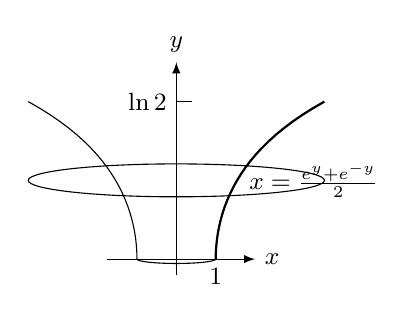
\begin{tikzpicture}[xscale=0.5,font=\small,declare function={f(\x)=1/2*(e^(\x)+e^(-\x));}]
\pgfmathsetmacro{\r}{f(2)}
\pgfmathsetmacro{\ra}{f(0)}
\pgfmathsetmacro{\ya}{ln(2)}
\draw[-latex](-1.75,0)--(2,0)node[right]{$x$};
\draw[-latex](0,-0.2)--(0,2.5)node[above]{$y$};
\draw[thick]plot[domain=0:2]({f(\x)},\x);
\draw[]plot[domain=0:2]({-f(\x)},\x);
\draw(1,0)node[below]{$1$};
\draw(0,\x) circle (\r cm and 1/18*\r cm);
\draw([shift={(180:\ra cm and 1/18*\ra cm)}]0,0) arc (180:360:\ra cm and 1/18*\ra cm);
\draw(0,2)node[left]{$\ln 2$}--++(0.4,0);
\draw(1,1)node[right,xshift=2ex]{$x=\frac{e^y+e^{-y}}{2}$};
\end{tikzpicture}
\caption{برائے سوال \حوالہ{سوال_ماورائی_سطح_طواف_رقبہ}}
\label{شکل_سوال_ماورائی_سطح_طواف_رقبہ}
\end{minipage}
\end{figure}
\ابتدا{سوال}
تفاعل \عددی{f(x)=x^2\ln\tfrac{1}{x}} کی مطلق زیادہ سے زیادہ قیمت تلاش کریں۔ یہ قیمت کہاں پائی جاتی ہے۔\\
جواب:\quad
\عددی{x=\tfrac{1}{\sqrt{e}}} پر مطلق زیادہ سے زیادہ \عددی{\tfrac{1}{2e}}
\انتہا{سوال}
%===================
\ابتدا{سوال}
تفاعل \عددی{f(x)=(x-3)^2e^x} اور اس کا ایک رتبی تفرق ایک ساتھ ترسیم کریں۔ \عددی{f'} کی قیمت اور علامت کے لحاظ سے \عددی{f} کے رویہ پر تبصرہ کریں۔ احصاء کی مدد سے ترسیم پر نمایاں نقطوں کی نشاندہی کریں۔
\انتہا{سوال}
%=====================
\ابتدا{سوال}
ربع اول میں بالائی جانب قوس \عددی{y=e^{2x}}، نچلی جانب قوس \عددی{y=e^x} اور دائیں جانب لکیر \عددی{x=\ln 3} میں محیط تکونی رقبہ تلاش کریں۔ \\
جواب:\quad
$2$
\انتہا{سوال}
%=======================
\ابتدا{سوال}
ربع اول میں بالائی جانب قوس \عددی{y=e^{x/2}}، نچلی جانب قوس \عددی{y=e^{-x/2}} اور دائیں جانب لکیر \عددی{x=2\ln 2} میں محیط تکونی رقبہ تلاش کریں۔ 
\انتہا{سوال}
%=======================
\ابتدا{سوال}
مستوی \عددی{xy} میں مبدا سے گزرتی وہ قوس  تلاش کریں جس کی لمبائی \عددی{x=0} سے \عددی{x=1} تک \عددی{L=\int_0^1\sqrt{1+\tfrac{e^x}{4}}\dif x} ہے۔\\
جواب:\quad
$y=e^{x/2}-1$
\انتہا{سوال}
%========================
\ابتدا{سوال}\شناخت{سوال_ماورائی_سطح_طواف_رقبہ}
منحنی \عددی{x=\tfrac{e^y+e^{-y}}{2},\,0\le y\le \ln 2} کو محور \عددی{y} کے گرد گھما کر سطح طواف پیدا کیا جاتا ہے (شکل \حوالہ{شکل_سوال_ماورائی_سطح_طواف_رقبہ})۔ اس سطح کا رقبہ تلاش کریں۔
\انتہا{سوال}
%========================
\ابتدا{سوال}
(ا) دکھائیں \عددی{\int\ln x\dif x=x\ln x-x+C}، (ب) وقفہ \عددی{[1,e]} پر \عددی{\ln x} کی اوسط قیمت تلاش کریں۔\\
جواب:\quad
(ا) \عددی{\tfrac{\dif}{\dif x}(x\ln x-x+C)=x\cdot\tfrac{1}{x}+\ln x-1+0=\ln x}، (ب) \عددی{\tfrac{1}{e-1}}
\انتہا{سوال}
%====================
\ابتدا{سوال}
وقفہ \عددی{[1,2]} پر \عددی{f(x)=\tfrac{1}{x}} کی اوسط قیمت تلاش کریں۔
\انتہا{سوال}
%====================
\ابتدا{سوال}\ترچھا{نقطہ $x=0$ پر $e^x$ کی خط بندی}\\
\begin{enumerate}[a.]
\item
نقطہ \عددی{x=0} پر خط بندی \عددی{e^x\approx 1+x} حاصل کریں۔
\item
وقفہ \عددی{[0,0.2]} پر \عددی{e^x} کی جگہ \عددی{1+x} استعمال کرنے سے پیدا خلل کو \عددی{5} اعشاریہ تک تلاش کریں۔
\item
وقفہ \عددی{-2\le x\le 2} پر \عددی{e^x} اور \عددی{1+x} کو ایک ساتھ کمپیوٹر پر ترسیم کریں۔ کس وقفہ پر تخمین زیادہ قیمت دیتی ہے؟  کم قیمت دیتی ہے؟
\end{enumerate}
جواب:\quad
(ب) حتمی خلل تقریباً \عددی{0.02140}
\انتہا{سوال}
%====================
\ابتدا{سوال}\شناخت{سوال_ماورائی_قواعد_قوت_نما}\ترچھا{قواعد قوت نما}\\
\begin{enumerate}[a.]
\item
مساوات \عددی{e^{x_1}e^{x_2}=e^{x_1+x_2}} جس کو اس حصہ میں حاصل کیا گیا، سے شروع کر کے دکھائیں کہ کسی بھی حقیقی عدد \عددی{x} کے لئے \عددی{e^{-x}=\tfrac{1}{e^x}} ہو گا۔ اس کے بعد کسی بھی دو اعداد \عددی{x_1} اور \عددی{x_2} کے لئے دکھائیں کہ \عددی{\tfrac{e_{x_1}}{e^{x_2}}=e^{x_1-x_2}} ہو گا۔
\item
کسی بھی دو اعداد \عددی{x_1} اور \عددی{x_2} کے لئے دکھائیں کہ \عددی{(e^{x_1})^{x_2}=e^{x_1x_2}=(e^{x_2})^{x_1}} ہو گا۔
\end{enumerate}
\انتہا{سوال}
%==================
\ابتدا{سوال}\ترچھا{$e$ کا اعشاری اظہار}\\
مساوات\عددی{\ln x=1} کو حل کرتے ہوئے \عددی{e} کی قیمت اتنے اعشاریہ تک تلاش کریں جتنے تک آپ کا کیلکولیٹر استعمال کرتے ہوئے ممکن ہو۔\\
جواب:\quad
$\num{2.71828183}$  
\انتہا{سوال}
%=====================
\ابتدا{سوال}\ترچھا{$\ln x$ اور $e^x$ کے مابین الٹ تعلق}\\
کیلکولیٹر استعمال کرتے ہوئے مرکبات \عددی{e^{\ln x}} اور \عددی{\ln(e^x)} کی قیمت تلاش کریں۔
\انتہا{سوال}
%=======================
\ابتدا{سوال}\شناخت{سوال_ماورائی_قوت_نما_تعلق_الف}
دکھائیں کہ کسی بھی عدد \عددی{a>1} کے لئے درج ذیل ہو گا (شکل \حوالہ{شکل_سوال_ماورائی_قوت_نما_تعلق_الف})۔
\begin{align*}
\int_16a\ln x\dif x+\int_0^{\ln a}e^y\dif y=a\ln a
\end{align*}
\انتہا{سوال}
%============
\begin{figure}
\centering
\begin{minipage}{0.45\textwidth}
\centering
\begin{tikzpicture}[font=\small,declare function={f(\x)=ln(\x);}]
\pgfmathsetmacro{\a}{2}
\pgfmathsetmacro{\b}{ln(\a)}
\begin{axis}[small,axis lines=middle,xlabel={$x$},ylabel={$y$},xlabel style={at={(current axis.right of origin)},anchor=west},ylabel style={at={(current axis.above origin)},anchor=south},xtick={1,\a},xticklabels={$1$,$a$},ytick={\b},yticklabels={$\ln a$},xmin=0,axis on top=true]
\fill[lgray](0,0) rectangle (\a,\b);
\addplot[domain=0.5:3]{f(x)}node[pos=0.85,left,yshift=1ex]{$y=\ln x$};
\draw(\a,0)--(\a,\b)--(0,\b);
\end{axis}
\end{tikzpicture}
\caption{ترسیم برائے سوال \حوالہ{سوال_ماورائی_قوت_نما_تعلق_الف}}
\label{شکل_سوال_ماورائی_قوت_نما_تعلق_الف}
\end{minipage}\hfill
\begin{minipage}{0.45\textwidth}
\centering
\begin{tikzpicture}[font=\small,declare function={f(\x)=\x^3;g(\x)=3.375+6.75*(\x-1.5);}]
\pgfmathsetmacro{\a}{1.2}
\pgfmathsetmacro{\b}{1.8}
\pgfmathsetmacro{\c}{1/2*(\a+\b)}
\begin{axis}[small,axis lines=middle,xlabel={$x$},ylabel={$y$},xlabel style={at={(current axis.right of origin)},anchor=west},ylabel style={at={(current axis.above origin)},anchor=south},xtick={\a,\b,\c},xticklabels={$\ln a$,$\ln b$,$\tfrac{\ln a+\ln b}{2}$},ymin=0,axis on top=true, axis y line=none]
\addplot[domain=1:2]{f(x)}node[pos=0.85,above left]{$y=e^x$};
\draw[name path=kL,dashed](\a,0)--(\a,{f(\a)})node[above]{$E$};
\draw[name path=kR,dashed](\b,0)--(\b,{f(\b)})node[above]{$F$};
\draw(\c,{f(\c)})coordinate[](kT)node[circ]{}node[below]{$M$};
\draw(\a,{f(\a)})--(\b,{f(\b)});
\addplot[domain=\a:\b]{g(x)};
\draw(\a,{g(\a)})node[left,yshift=-1ex]{$B$} (\b,{g(\b)})node[right]{$C$}  (\a,0)node[above right]{$A$}  (\b,0)node[above left]{$D$};
\end{axis}
\end{tikzpicture}
\caption{ترسیم برائے سوال \حوالہ{سوال_ماورائی_قوت_نما_تعلق_ب}}
\label{شکل_سوال_ماورائی_قوت_نما_تعلق_ب}
\end{minipage}
\end{figure}
\ابتدا{سوال}\شناخت{سوال_ماورائی_قوت_نما_تعلق_ب}\ترچھا{تکونیاتی، لوگارتھمی اور حسابی اوسط عدم مساوات}\\
\begin{enumerate}[a.]
\item
دکھائیں کہ \عددی{x} کے ہر وقفہ پر \عددی{e^x} کی ترسیم مقعر اوپر ہے۔
\item
اگر \عددی{0<a<b} ہو تب دکھائیں کہ درج ذیل ہو گا (شکل \حوالہ{شکل_سوال_ماورائی_قوت_نما_تعلق_ب})۔
\begin{align*}
e^{(\ln a+\ln b)/2}\cdot(\ln b-\ln a)<\int_{\ln a}^{\ln b} e^x\dif x<\frac{e^{\ln a}+e^{\ln b}}{2}\cdot (\ln b-\ln a)
\end{align*}
\item
جزو-ب کی عدم مساوات کو استعمال کرتے ہوئے  درج ذیل کی تصدیق کریں۔
\begin{align*}
\sqrt{ab}<\frac{b-1}{\ln b-\ln a}<\frac{a+b}{2}
\end{align*}
یہ عدم مساوات کہتی ہے کہ دو مثبت اعداد کا ہندسی اوسط ان کے لوگارتھمی اوسط سے کم ہو گا جو از خود ان کی حسابی اوسط سے کم ہو گا۔
\end{enumerate}
\انتہا{سوال}
%=========================

\حصہ{$a^x$ \, اور \, $\log_a x$}
اب تک ماسوائے \عددی{e} کے ہم نے مثبت اعداد کو غیر ناطق طاقت دینا نہیں سیکھا ہے۔ قوت نمائی تفاعل کی تعریف \عددی{e^x=\ln^{-1}x}، متغیر  \عددی{x} کی تمام حقیقی قیمتوں، ناطق اور غیر ناطق،  کے لئے درست ہے۔ اس حصہ میں ہم اس تعریف کو استعمال کر کے کسی بھی مثبت عدد کو کسی بھی ناطق یا غیر ناطق کی طاقت دینا سیکھ کر مثبت عدد \عددی{a} کے لئے قوت نمائی تفاعل \عددی{y=a^x} کی تعریف پیش کریں گے۔ اس کے ساتھ ساتھ ہم تفرق کے طاقتی قاعدہ کو حتمی شکل دیں گے (جو تمام قوت نما کے لئے درست ہو گا) اور ایک تفاعل کو دوسرے تفاعل کی طاقت دیں گے مثلاً \عددی{x^x} اور \عددی{(\sin x)^{\tan x}}، وغیرہ۔

جیسا \عددی{e^x} بہت سارے قوت نما تفاعل میں سے ایک ہے، اسی طرح \عددی{\ln x} بھی بہت سارے لوگارتھمی تفاعل،جو تفاعل \عددی{a^x} کے الٹ ہیں،  میں سے ایک ہے۔

\جزوحصہء{تفاعل $a^x$}
چونکہ کسی بھی مثبت عدد \عددی{a} کے لئے \عددی{a=e^{\ln a}} ہوتا ہے لہٰذا  ہم \عددی{a^x} کو \عددی{(e^{\,\ln a})^x=e^{\,x\ln a}} تصور کر سکتے ہیں۔ یوں ہم درج ذیل تعریف پیش کرتے ہیں۔
\begin{align}
a^x&=e^{\,x\ln a},\quad\quad a>0 &&\text{تعریف}
\end{align}

\ابتدا{مثال}
\begin{align*}
\text{(ا)}\quad 2^{\sqrt{3}}&=e^{\,\sqrt{3}\ln 2}\\
\text{(ب)}\quad 2^{\pi}&=e^{\pi\ln 2}
\end{align*}
\انتہا{مثال}
%=======================
تفاعل\عددی{a^x} قوت نما کے عمومی قواعد جنہیں جدول \حوالہ{جدول_ماورائی_قوت_نما_عمومی_قواعد} میں پیش کیا گیا ہے کو مطمئن کرتا ہے۔ ہم ان قواعد کے ثبوت پیش نہیں کریں گے۔
\begin{table}
\caption{قواعد برائے قوت نما}
\label{جدول_ماورائی_قوت_نما_عمومی_قواعد}
\centering
\renewcommand{\arraystretch}{2} 
\begin{tabular}{c|l}
\toprule
\multicolumn{2}{c}{$a>0$ ہے جبکہ $x$ اور $y$ کوئی بھی اعداد ہو سکتے ہیں}\\
\midrule
ا&$a^x\cdot a^y=a^{x+y}$\\
ب&$a^{-x}=\frac{1}{a^x}$\\
ج&$\frac{a^x}{a^y}=a^{x-y}$\\
د&$(a^x)^y=a^{xy}=(a^y)^x$\\
\bottomrule
\end{tabular}
\end{table}

\جزوحصہء{قاعدہ طاقت (حتمی صورت)}
اساس \عددی{a} کے لوگارتھم کا تفرق حاصل کرنے کی خاطر ہمیں اس کو پہلے  قدرتی لوگارتھم  کی صورت میں لکھتے ہیں۔ اگر \عددی{u} متغیر \عددی{x} کا مثبت قابل تفرق تفاعل ہو تب
\begin{align*}
\frac{\dif}{\dif x}(\log_a u)=\frac{\dif}{\dif x}\big(\frac{\ln u}{\ln a}\big)=\frac{1}{\ln a}\cdot\frac{1}{u}\frac{\dif u}{\dif x}
\end{align*}
یعنی
\begin{align}
\frac{\dif}{\dif x}(\log_a u)=\frac{1}{\ln a}\cdot\frac{1}{u}\frac{\dif u}{\dif x}
\end{align}
ہو گا۔

\ابتدا{مثال}
\begin{align*}
\frac{\dif}{\dif x}\log_{10}(3x+1)=\frac{1}{\ln 10}\cdot\frac{1}{3x+1}\frac{\dif}{\dif x}(3x+1)=\frac{3}{(\ln 10)(3x+1)}
\end{align*}
\انتہا{مثال}
%===============
\جزوحصہء{تکمل جہاں \عددی{\log_a x} پایا جاتا ہو}
جب اساس \عددی{a} کا لوگارتھم پایا جاتا ہو تب تکمل لیتے ہوئے ہم اس کو پہلے قدرتی لوگارتھم کی صورت میں بدلتے ہیں۔

\ابتدا{مثال}
\begin{align*}
\int\frac{\log_2x}{x}\dif x&=\frac{1}{\ln 2}\int\frac{\ln x}{x}\dif x&&\log_2x=\frac{\ln x}{\ln 2}\\
&=\frac{1}{\ln 2}\int u\dif u&&u=\ln x\\
&=\frac{1}{\ln 2}\frac{u^2}{2}+C\\
&=\frac{1}{\ln 2}\frac{(\ln x)^2}{2}+C=\frac{(\ln x)^2}{2\ln 2}+C
\end{align*}
\انتہا{مثال}
%===================
\جزوحصہء{اساس $10$ لوگارتھم}
اساس \عددی{10} لوگارتھم جس کو \اصطلاح{عام لوگارتھم}\فرہنگ{لوگارتھم!عام}\حاشیہب{common logarithm}\فرہنگ{logarithm!common} کہتے ہیں کئی سائنسی کلیات میں پایا جاتا ہے۔ مثال کے طور پر زلزلہ کی شدت کو عموماً اساس \عددی{10} کے  لوگارتھمی\حاشیہد{رکٹر پیمائش میں اکائی کا اضافہ حیطہ میں تقریباً \عددیء{10} گنّا  اور توانائی میں تقریباً \عددی{31.623} گنّا کا اضافہ ظاہر کرتا ہے۔} \اصطلاح{رکٹر پیمائش}\فرہنگ{رکٹر پیمائش}\فرہنگ{پیما!رکٹر}\حاشیہب{Richter scale}\فرہنگ{Richter scale} میں پیش جاتا ہے۔ رکٹر پیما کا کلیہ 
\begin{align*}
\text{شدت}\, R=\log_{10}\big(\frac{a}{T}\big)+B
\end{align*}
ہے جہاں زلزلہ پیما کے مقام پر زمینی لرزش کا حیطہ \عددی{a} ہے جس کو مائیکرو میٹر میں ناپا جاتا ہے، زلزلہ کی موج کا دوری عرصہ \عددی{T} ہے جس کو سیکنڈ میں ناپا جاتا ہے جبکہ \عددی{B} ایک تجربی جزو ہے جو مرکز زلزلہ اور زلزلہ پیما کے بیچ شدت کی کمی کو ظاہر کرتا ہے۔ 

جاپان کے شہر ناگاساکی پر گرائے  گئے ایٹمی بم میں \عددی{\SI{1.34e14}{\joule}}  توانائی تھی جو رکٹر پیما پر \عددی{5} کے برابر ہے۔  آج تک سب سے بڑا ایٹمی دھماکہ \عددی{7.1} شدت کا تھا جس میں \عددی{\SI{2.09e17}{\joule}} توانائی تھی۔  اکتوبر 8 \سن{2005} کو آزاد کشمیر میں \عددی{7.6} شدت کا زلزلہ آیا جس میں \عددی{\SI{1.585e16}{\joule}} توانائی تھی۔

\ابتدا{مثال}
مرکز زلزلہ سے زلزلہ پیما تک فاصلہ \عددی{\SI{10000}{\kilo\meter}} ہے جس کے لئے \عددی{B=6.8} ہو گا۔ مقام زلزلہ پیما پر زمین کی انتصابی حرکت \عددی{\SI{10}{\micro\meter}} اور دوری عرصہ \عددی{\SI{1}{\second}} ہیں۔ زلزلہ کی شدت تلاش کریں۔

حل:\quad
\begin{align*}
R=\log_{10}\big(\frac{10}{1}\big)+6.8=1+6.8=7.8
\end{align*}
\انتہا{مثال}
%====================
محلول کی تیزابیت\فرہنگ{تیزابیت} کو \عددی{\pH} (\اصطلاح{طاقت ہائیڈروجن})\فرہنگ{pH}\فرہنگ{طاقت!ہائیڈروجن} میں ناپا جاتا ہے جو اساس \عددی{10} کا لوگارتھمی پیمانہ\حاشیہد{$\pH$ کی جدید تعریف کے تحت اس کو "مخفی قوہ ہائیڈروجن" کہنا زیادہ بہتر ہو گا۔} ہے۔ محلول میں ہائیڈرونیم برق پارہ \عددی{[\ce{H3O^+}]} کے گھنا پن کے بالعکس کا عام لوگارتھم  اس محلول کی \عددی{\pH} قیمت ہو گی:
\begin{align*}
\pH=\log_{10}\frac{1}{[\ce{H3O^+}]}=-\log_{10}[\ce{H3O^+}]
\end{align*}
ہائیڈرونیم برق پارہ کے گھنا پن کو مول فی لٹر (\si{\mole\per\liter}) میں ناپا جاتا ہے۔تیزاب کی \عددی{\pH} قیمت \عددی{7} سے کم جبکہ القلی کی  \عددی{7} سے زیادہ ہوتی ہے۔ سرکہ کی \عددی{\pH} قیمت \عددی{3} جبکہ مقطر پانی کی \عددی{\pH} قیمت \عددی{7} ہوتی ہے۔  \عددی{\pH}  کا  پیمانہ \عددی{0} سے \عددی{14} تک ہوتا ہے۔ جدول \حوالہ{جدول_ماورائی_خوراک_ہائیڈروجن_مخفی_قوہ} میں کئی اجزاء کی \عددی{\pH} دی گئی ہے۔
\begin{table}
\caption{عمومی خوراک کی $\pH<7$ ہے۔}
\label{جدول_ماورائی_خوراک_ہائیڈروجن_مخفی_قوہ}
\centering
\begin{tabular}{rr}
\toprule
خوراک& \multicolumn{1}{c}{$\pH$}\\
\midrule
کیلا& \عددی{4.5-4.7}\\
چکوترہ& \عددی{3.0-3.3}\\
سنترا & \عددی{3.0-4.0}\\
لیموں& \عددی{1.8-2.0}\\
دودھ&\عددی{6.3-6.6}\\
مرچ&\عددی{5.1-5.7}\\
\bottomrule
\end{tabular}
\end{table}

لوگارتھم کی ایک اور مثال ڈیسی بیل \عددی{\si{\deci\bel}} پیمانہ ہے جو صدا کی بلندی کو ناپنے کے لئے استعمال کیا جاتا ہے۔ اگر صدا کی شدت \عددی{I}  واٹ فی مربع میٹر ہو تب
\begin{align}\label{مساوات_ماورائی_سطح_صدا}
\text{\RL{سطح صدا}}=10\log_{10}(I\times 10^{12})\,\si{\deci\bel}
\end{align}
ہو گا۔ جیسا اگلا مثال دکھاتا ہے، شدت صدا کو دگنا کرنے سے سطح صدا میں تقریباً \عددی{\SI{3}{\deci\bel}} کا اضافہ ہوتا ہے۔

\ابتدا{مثال}
صدا کی شدت کو دگنا کرنے سے سطح صدا میں کتنا اضافہ ہو گا؟

حل:\quad
مساوات \حوالہ{مساوات_ماورائی_سطح_صدا} کے تحت \عددی{2I} شدت صدا کے لئے 
\begin{align*}
\text{\RL{دگنی شدت کی سطح صدا}}&=10\log_{10}(2I\times 10^{12})&&\text{\RL{مساوات \حوالہ{مساوات_ماورائی_سطح_صدا} میں $2I$}}\\
&=10\log_{10}2+10\log_{10}(I\times 10^{12})\\
&=\text{\RL{اصل شدت کی سطح صدا}}+10\log_{10}2\\
&\approx \text{\RL{اصل شدت کی سطح صدا}}+3   && \log_{10}\approx 0.3
\end{align*}
ہو گا۔
\انتہا{مثال}
%======================
سطح صدا کی چند قیمتیں جدول \حوالہ{جدول_ماورائی_شدت_صدا} میں دی گئی ہیں۔
\begin{table}
\caption{سطح صدا کی چند قیمتیں۔}
\label{جدول_ماورائی_شدت_صدا}
\centering
\begin{tabular}{rr}
\toprule
سماعت کی کمتر سطح & \عددی{\SI{0}{\deci\bel}}\\
پتوں کا سرسرانا & \عددی{\SI{10}{\deci\bel}}\\
سرگوشی& \عددی{\SI{20}{\deci\bel}}\\
خاموش گاڑی& \عددی{{50}{\deci\bel}}\\
عام بات چیت& \عددی{\SI{65}{\deci\bel}}\\
تین میٹر دور ہوائی برما & \عددی{\SI{90}{\deci\bel}}\\
کانوں میں درد& \عددی{\SI{120}{\deci\bel}}\\
\bottomrule
\end{tabular}
\end{table}



\حصہء{سوالات}
\موٹا{الجبرائی حساب}

سوال \حوالہ{سوال_ماورائی_سادہ_صورت_فقرہ_الف} تا سوال \حوالہ{سوال_ماورائی_سادہ_صورت_فقرہ_ب} میں ریاضی فقرے کی سادہ صورت تلاش کریں۔

\ابتدا{سوال}\شناخت{سوال_ماورائی_سادہ_صورت_فقرہ_الف}
\begin{multicols}{3}
\begin{enumerate}[a.]
\item
$5^{\log_57}$
\item
$8^{\log_8\sqrt{2}}$
\item
$1.3^{\log_{1.3}75}$
\item
$\log_416$
\item
$\log_3\sqrt{3}$
\item
$\log_4\big(\frac{1}{4}\big)$
\end{enumerate}
\end{multicols}
\انتہا{سوال}
%========================
\ابتدا{سوال}
\begin{multicols}{3}
\begin{enumerate}[a.]
\item
$2^{\log_2 3}$
\item
$10^{\log_{10}(1/2)}$
\item
$\pi^{\log_{\pi}7}$
\item
$\log_{11}121$
\item
$\log_{121}11$
\item
$\log_3\big(\frac{1}{9}\big)$
\end{enumerate}
\end{multicols}
\انتہا{سوال}
%========================
\ابتدا{سوال}
\begin{multicols}{3}
\begin{enumerate}[a.]
\item
$2^{\log_4 x}$
\item
$9^{\log 3 x}$
\item
$\log_2(e^{(\ln 2)(\sin x)})$
\end{enumerate}
\end{multicols}
\انتہا{سوال}
%========================
\ابتدا{سوال}\شناخت{سوال_ماورائی_سادہ_صورت_فقرہ_ب}
\begin{multicols}{3}
\begin{enumerate}[a.]
\item
$25^{\log_5(3x^2)}$
\item
$\log_e(e^x)$
\item
$\log_4(2^{e^x\sin x})$
\end{enumerate}
\end{multicols}
\انتہا{سوال}
%========================
سوال \حوالہ{سوال_ماورائی_قدرتی_لوگاتمی_سادہ_الف} اور سوال \حوالہ{سوال_ماورائی_قدرتی_لوگاتمی_سادہ_ب} میں نسبت کو قدرتی لوگارتھمی صورت میں لکھ کر سادہ صورت حاصل کریں۔

\ابتدا{سوال}\شناخت{سوال_ماورائی_قدرتی_لوگاتمی_سادہ_الف}
\begin{multicols}{3}
\begin{enumerate}[a.]
\item
$\tfrac{\log_2x}{\log_3x}$
\item
$\tfrac{\log_2x}{\log_8x}$
\item
$\tfrac{\log_xa}{\log_{x^2}a}$
\end{enumerate}
\end{multicols}
\انتہا{سوال}
%====================
\ابتدا{سوال}\شناخت{سوال_ماورائی_قدرتی_لوگاتمی_سادہ_ب}
\begin{multicols}{3}
\begin{enumerate}[a.]
\item
$\tfrac{\log_9x}{\log_3x}$
\item
$\tfrac{\log_{\sqrt{10}}x}{\log_{\sqrt{2}}x}$
\item
$\tfrac{\log_ab}{\log_ba}$
\end{enumerate}
\end{multicols}
\انتہا{سوال}
%====================
سوال \حوالہ{سوال_ماورائی_مساوات_حل_الف} تا سوال \حوالہ{سوال_ماورائی_مساوات_حل_ب} میں دی گئی مساوات حل کریں۔

\ابتدا{سوال}\شناخت{سوال_ماورائی_مساوات_حل_الف}
$3^{\log_3(7)+2^{\log_2(5)}}=5^{\log_5(x)}$
\انتہا{سوال}
%==================
\ابتدا{سوال}
$8^{\log_8(3)}-e^{\ln 5}=x^2-7^{\log_7(3x)}$
\انتہا{سوال}
%=====================
\ابتدا{سوال}
$3^{\log_3(x^2)=5e^{\ln x}}-3\cdot 10^{\log_{10}(2)}$
\انتہا{سوال}
%====================
\ابتدا{سوال}\شناخت{سوال_ماورائی_مساوات_حل_ب}
 $\ln e+4^{-2\log_4(x)}=\frac{1}{x}\log_{10}(100)$
\انتہا{سوال}
%==================
سوال \حوالہ{سوال_ماورائی_تفرق_بالحظ_تلاش_الف} تا سوال \حوالہ{سوال_ماورائی_تفرق_بالحظ_تلاش_ب} میں دیے گئے غیر تابع متغیر کے لحاظ سے \عددی{y} کا تفرق تلاش کریں۔

\ابتدا{سوال}\شناخت{سوال_ماورائی_تفرق_بالحظ_تلاش_الف}
$y=2^x$
\انتہا{سوال}
%==========================
\ابتدا{سوال}
$y=3^{-x}$
\انتہا{سوال}
%==========================
\ابتدا{سوال}
$y=5^{\sqrt{s}}$
\انتہا{سوال}
%==========================
\ابتدا{سوال}
$y=2^{s^2}$
\انتہا{سوال}
%==========================
\ابتدا{سوال}
$y=x^{\pi}$
\انتہا{سوال}
%==========================
\ابتدا{سوال}
$y=t^{1-e}$
\انتہا{سوال}
%==========================
\ابتدا{سوال}
$y=(\cos\theta)^{\sqrt{2}}$
\انتہا{سوال}
%==========================
\ابتدا{سوال}
$y=(\ln\theta)^{\pi}$
\انتہا{سوال}
%==========================
\ابتدا{سوال}
$y=7{\sec\theta}\ln 7$
\انتہا{سوال}
%==========================
\ابتدا{سوال}
$y=3^{\tan\theta}\ln 3$
\انتہا{سوال}
%==========================
\ابتدا{سوال}
$y=2^{\sin 3t}$
\انتہا{سوال}
%==========================
\ابتدا{سوال}
$y=5^{-\cos 2t}$
\انتہا{سوال}
%==========================
\ابتدا{سوال}
$y=\log_25\theta$
\انتہا{سوال}
%==========================
\ابتدا{سوال}
$y=\log_3(1+\theta\ln 3)$
\انتہا{سوال}
%==========================
\ابتدا{سوال}
$y=\log_4x+\log_4x^2$
\انتہا{سوال}
%==========================
\ابتدا{سوال}
$y=\log_{25}e^x-\log_5\sqrt{x}$
\انتہا{سوال}
%==========================
\ابتدا{سوال}
$y=\log_2r\cdot\log_4r$
\انتہا{سوال}
%==========================
\ابتدا{سوال}
$y=\log_3r\cdot\log_9r$
\انتہا{سوال}
%==========================
\ابتدا{سوال}
$y=\log_3\big((\tfrac{x+1}{x-1})^{\ln 3}\big)$
\انتہا{سوال}
%==========================
\ابتدا{سوال}
$y=\log_5\sqrt{(\tfrac{7x}{3x+2})^{\ln 5}}$
\انتہا{سوال}
%==========================
\ابتدا{سوال}
$y=\theta\sin(\log_7\theta)$
\انتہا{سوال}
%==========================
\ابتدا{سوال}
$y=\log_7(\tfrac{\sin\theta\cos\theta}{e^{\theta}2^{\theta}})$
\انتہا{سوال}
%==========================
\ابتدا{سوال}
$y=\log_5e^x$
\انتہا{سوال}
%==========================
\ابتدا{سوال}
$y=\log_2(\tfrac{x^2e^2}{2\sqrt{x+1}})$
\انتہا{سوال}
%==========================
\ابتدا{سوال}
$y=3^{\log_2 t}$
\انتہا{سوال}
%==========================
\ابتدا{سوال}
$y=3\log_8(\log_2t)$
\انتہا{سوال}
%==========================
\ابتدا{سوال}
$y=\log_2(8t^{\ln 2})$
\انتہا{سوال}
%==========================
\ابتدا{سوال}\شناخت{سوال_ماورائی_تفرق_بالحظ_تلاش_ب}
$y=t\log_3(e^{(\sin t)(\ln 3)})$
\انتہا{سوال}
%==========================
\موٹا{لوگارتھمی تفرق}

سوال \حوالہ{سوال_ماورائی_لوگارتھمی_تفرق_الف} تا سوال \حوالہ{سوال_ماورائی_لوگارتھمی_تفرق_ب} میں \عددی{y} کا لوگارتھمی تفرق دیے گئے غیر تابع متغیر کے لحاظ سے معلوم کریں۔ 

\ابتدا{سوال}\شناخت{سوال_ماورائی_لوگارتھمی_تفرق_الف}
$y=(x+1)^x$
\انتہا{سوال}
%======================
\ابتدا{سوال}
$y=x^{(x+1)}$
\انتہا{سوال}
%======================
\ابتدا{سوال}
$y=(\sqrt{t})^t$
\انتہا{سوال}
%======================
\ابتدا{سوال}
$y=t^{\sqrt{t}}$
\انتہا{سوال}
%======================
\ابتدا{سوال}
$y=(\sin x)^x$
\انتہا{سوال}
%======================
\ابتدا{سوال}
$y=x^{\sin x}$
\انتہا{سوال}
%======================
\ابتدا{سوال}
$y=x^{\ln x}$
\انتہا{سوال}
%======================
\ابتدا{سوال}\شناخت{سوال_ماورائی_لوگارتھمی_تفرق_ب}
$y=(\ln x)^{\ln x}$
\انتہا{سوال}
%======================
\موٹا{تکمل}\\
سوال \حوالہ{سوال_ماورائی_تکمل_تلاش_کریں-الف} تا سوال \حوالہ{سوال_ماورائی_تکمل_تلاش_کریں-ب} میں تکمل تلاش کریں۔

\ابتدا{سوال}\شناخت{سوال_ماورائی_تکمل_تلاش_کریں-الف}
$\int5^x\dif x$
\انتہا{سوال}
%======================
\ابتدا{سوال}
$\int(1.3)^x\dif x$
\انتہا{سوال}
%======================
\ابتدا{سوال}
$\int_0^12^{-\theta}\dif \theta$
\انتہا{سوال}
%======================
\ابتدا{سوال}
$\int_{-2}^05^{-\theta}\dif \theta$
\انتہا{سوال}
%======================
\ابتدا{سوال}
$\int_1^{\sqrt{2}}x2^{(x^2)}\dif x$
\انتہا{سوال}
%======================
\ابتدا{سوال}
$\int_1^4 \frac{2^{\sqrt{x}}}{\sqrt{x}}\dif x$
\انتہا{سوال}
%======================
\ابتدا{سوال}
$\int_0^{\pi/2}7^{\cos t}\sin t\dif t$
\انتہا{سوال}
%======================
\ابتدا{سوال}
$\int_0^{\pi/4}\big(\frac{1}{3}\big)^{\tan t}\sec^2t\dif t$
\انتہا{سوال}
%======================
\ابتدا{سوال}
$\int_2^4x^{2x}(1+\ln x)\dif x$
\انتہا{سوال}
%======================
\ابتدا{سوال}\شناخت{سوال_ماورائی_تکمل_تلاش_کریں-ب}
$\int_1^2\frac{2^{\ln x}}{x}\dif x$
\انتہا{سوال}
%======================
سوال \حوالہ{سوال_ماورائی_تکمل_حل_کریں_الف} تا سوال \حوالہ{سوال_ماورائی_تکمل_حل_کریں_ب} میں دیے گئے تکمل حل کریں۔

\ابتدا{سوال}\شناخت{سوال_ماورائی_تکمل_حل_کریں_الف}
$\int 3x^{\sqrt{3}}\dif x$
\انتہا{سوال}
%====================
\ابتدا{سوال}
$\int x^{\sqrt{2}-1}\dif x$
\انتہا{سوال}
%====================
\ابتدا{سوال}
$\int_0^3(\sqrt{2}+1)x^{\sqrt{2}}\dif x$
\انتہا{سوال}
%====================
\ابتدا{سوال}\شناخت{سوال_ماورائی_تکمل_حل_کریں_ب}
$\int_1^ex^{(\ln 2)-1}$
\انتہا{سوال}
%====================
سوال \حوالہ{سوال_ماورائی_دیا_تکمل_الف} تا سوال \حوالہ{سوال_ماورائی_دیا_تکمل_ب} میں دیے تکمل کو حل کریں۔

\ابتدا{سوال}\شناخت{سوال_ماورائی_دیا_تکمل_الف}
$\int\frac{\log_{10}x}{x}\dif x$
\انتہا{سوال}
%=======================
\ابتدا{سوال}
$\int_1^4\frac{\log_2 x}{x}\dif x$
\انتہا{سوال}
%=====================
\ابتدا{سوال}
$\int_1^4\frac{\ln 2\log_2 x}{x}\dif x$
\انتہا{سوال}
%=====================
\ابتدا{سوال}
$\int_1^e\frac{2\ln 10 \log_{10}x}{x}\dif x$
\انتہا{سوال}
%=================
\ابتدا{سوال}
$\int_0^2\frac{\log_2(x+2)}{x+2}\dif x$
\انتہا{سوال}
%===================
\ابتدا{سوال}
$\int_{1/10}^{10}\frac{\log_{10}(10x)}{x}\dif x$
\انتہا{سوال}
%===================
\ابتدا{سوال}
$\int_0^9\frac{2\log_{10}(x+1)}{x+1}\dif x$
\انتہا{سوال}
%===================
\ابتدا{سوال}
$\int_2^3\frac{2\log_2(x-1)}{x-1}\dif x$
\انتہا{سوال}
%===================
\ابتدا{سوال}
$\int\frac{\dif x}{x\log_{10}x}$
\انتہا{سوال}
%===================
\ابتدا{سوال}\شناخت{سوال_ماورائی_دیا_تکمل_ب}
$\int\frac{\dif x}{x(\log_8x)^2}$
\انتہا{سوال}
%===================
سوال \حوالہ{سوال_ماورائی_تکمل_کی_قیمت_الف} تا سوال \حوالہ{سوال_ماورائی_تکمل_کی_قیمت_ب} میں تکمل کی قیمت تلاش کریں۔

\ابتدا{سوال}\شناخت{سوال_ماورائی_تکمل_کی_قیمت_الف}
$\int_1^{\ln x}\frac{1}{t}\dif t,\quad x>1$
\انتہا{سوال}
%=====================
\ابتدا{سوال}
$\int_1^{e^x}\frac{1}{t}\dif t$
\انتہا{سوال}
%=====================
\ابتدا{سوال}
$\int_1^{1/x}\frac{1}{t}\dif t,\quad x>0$
\انتہا{سوال}
%=====================
\ابتدا{سوال}\شناخت{سوال_ماورائی_تکمل_کی_قیمت_ب}
$\frac{1}{\ln a}\int_1^x\frac{1}{t}\dif t,\quad x>0$
\انتہا{سوال}
%=====================
\موٹا{نظریہ اور استعمال}

\ابتدا{سوال}
منحنی \عددی{y=\tfrac{2x}{1+x^2}} اور محور \عددی{x} پر \عددی{-2\le x\le 2}  کے بیچ خطے کا رقبہ معلوم کریں۔
\انتہا{سوال}
%=====================
\ابتدا{سوال}
منحنی \عددی{y=2^{1-x}} اور محور \عددی{x} پر \عددی{-1\le x\le 1}  کے بیچ خطے کا رقبہ معلوم کریں۔
\انتہا{سوال}
%==========================
\ابتدا{سوال}\ترچھا{انسانی خون کا $\pH$}\\
انسانی خون کے \عددی{\pH} کی قیمت \عددی{7.37} سے \عددی{7.44} تک ہوتی ہے۔ انسانی خون میں برق پارہ \عددی{[\ce{H3O^+}]} کے مطابقتی حدود تلاش کریں۔ 
\انتہا{سوال}
%========================
\ابتدا{سوال}\ترچھا{دماغی سیال کا $\pH$}\\
دماغی سیال میں \عددی{[\ce{H3O^+}]} کا گاڑھا پن تقریباً \عددی{\SI{4.8e-8}{\mole\per\liter}} ہے۔ اس سیال کا \عددی{\pH} تلاش کریں۔
\انتہا{سوال}
%====================
\ابتدا{سوال}
افزائش کار (ایمپلی فائر) سے حاصل صدا کو جزو \عددی{k} سے ضرب دے کر اس سطح صدا کو \عددی{\SI{10}{\deci\bel}} مزید بلن کیا جاتا ہے۔ جزو \عددی{k} کی قیمت تلاش کریں۔
\انتہا{سوال}
%===================
\ابتدا{سوال}
ایک افزائش کار صدا کی شدت کو \عددی{10} سے ضرب دیتا ہے۔ صدا میں کتنے \عددی{\si{\deci\bel}} کا اضافہ پیدا ہو گا؟ 
\انتہا{سوال}
%===================
\ابتدا{سوال}
کسی بھی محلول میں \عددی{[\ce{H3O^+}]}  اور \عددی{[OH^-]} کی گاڑھا پن کا حاصل ضرب \عددی{10^{-14}} ہوتا ہے۔
\begin{enumerate}[a.]
\item
\عددی{[\ce{H3O^+}]} کی کیا قیمت گاڑھا پن کی مجموعی \عددی{S=[\ce{H3O^+}]+[\ce{OH^-}]} کو کم سے کم  کرتی ہے؟
\item
اس محلول کی \عددی{\pH} تلاش کریں  جس میں \عددی{S} کی قیمت کم سے کم ہو۔
\item
\عددی{[\ce{H3O^+}]} اور \عددی{[OH^-]} کی کون سی نسبت \عددی{S} کو کم سے کم بناتی ہے؟
\end{enumerate}
\انتہا{سوال}
%==================
\ابتدا{سوال}
کیا \عددی{\log_ab} کی قیمت \عددی{\tfrac{1}{\log_ba}} کے برابر ہو سکتی ہے؟ اپنے جواب کی وجہ   پیش کریں۔
\انتہا{سوال}
%===================
\موٹا{کمپیوٹر کا استعمال}

\ابتدا{سوال}
مساوات \عددی{x^2=2^x} کے دو حل \عددی{x=2} اور  \عددی{x=4} ہیں جبکہ اس کا تیسرا حل بھی پایا جاتا ہے۔ ترسیم کی مدد سے تیسرا حل تلاش کریں۔
\انتہا{سوال}
%===================
\ابتدا{سوال}
کیا \عددی{x>0} کے لئے  \عددی{x^{\ln 2}} اور \عددی{2^{\ln x}} ایک دوسرے کے برابر ہو سکتے ہیں؟دونوں تفاعل ترسیم کرتے ہوئے بتائیں کیا ہوتا ہے۔
\انتہا{سوال}
%====================
\ابتدا{سوال}\ترچھا{$2^x$ کی خط بندی}\\
(ا) نقطہ \عددی{x=0} پر \عددی{f(x)=2^x} کی خط بندی دریافت کریں۔ اس کے بعد عددی سروں کو \عددی{2} اعشاریہ  پور و پور کریں۔ (ب) وقفہ \عددی{-3\le x\le 3} اور وقفہ \عددی{-1\le x\le 1} کے لئے تفاعل اور خط بندی کو ایک ساتھ ترسیم کریں۔
\انتہا{سوال}
%===================
\ابتدا{سوال}\ترچھا{$f(x)=\log_3 x$ کی خط بندی}\\
(ا) نقطہ \عددی{x=3} پر \عددی{f(x)=\log_3 x} کی خط بندی تلاش کریں۔ اس کے بعد عددی سروں کو \عددی{2} اعشاریہ تک پور و پور کریں۔   (ب) وقفہ \عددی{0\le x\le 8} اور \عددی{2\le x\le} کے لئے تفاعل اور خط بندی کو ایک ساتھ ترسیم کریں۔
\انتہا{سوال}
%====================
\موٹا{دیگر اساس کے ساتھ حساب کتاب}

\ابتدا{سوال}
عموماً کیلکولیٹروں میں \عددی{\log_{10}x} اور \عددی{\ln x} پائے جاتے ہیں۔ دیگر اساس کے لوگارتھم تلاش کرنے کی خاطر ہم درج ذیل مساوات استعمال کرتے ہیں۔
\begin{align*}
\log_ax=\frac{\ln x}{\ln a}
\end{align*}
یوں درج ذیل ہو گا۔
\begin{align*}
\log_25=\frac{\ln 5}{\ln 2}\approx 2.3219
\end{align*}
کیلکولیٹر استعمال کرتے ہوئے  \عددی{5} اعشاریہ درستگی تک 
(ا) \عددی{\log_38}، (ب) \عددی{\log_70.5}، (ج) \عددی{\log_{2-}17}، (د) \عددی{\log_{0.5}7} تلاش کریں۔ درج ذیل معلومات استعمال کرتے ہوئے \عددی{\ln x} تلاش کریں۔
(ہ) \عددی{\log_{10}x=2.3}،  (و) \عددی{\log_2x=1.4}،  (ز) \عددی{\log_2x=-1.5}،  (ح) \عددی{\log_{10}x=-0.7}
\انتہا{سوال}
%=====================
\ابتدا{سوال}\ترچھا{تبدیلی پیمانہ}\\
(ا) دکھائیں کہ اساس \عددی{10} لوگارتھم کو اساس \عددی{2} لوگارتھم میں تبدیل کرنے کی مساوات درج ذیل ہے۔
\begin{align*}
\log_2x=\frac{\ln 10}{\ln 2}\log_{10}x
\end{align*}
(ب) دکھائیں کہ اساس  \عددی{a} لوگارتھم کو اساس \عددی{b} لوگارتھم میں تبدیل کرنے  کی مساوات درج ذیل ہے۔
\begin{align*}
\log_bx=\frac{\ln a}{\ln b}\log_ax
\end{align*}
\انتہا{سوال}
%=======================

\حصہ{افزائش اور تنزل}\شناخت{حصہ_ماورائی_افزائش_تنزل}
اس حصہ میں ہم قوت نما تبدیلی کے قاعدہ کو حاصل کریں گے۔ اس کے علاوہ ان عملی استعمال پر غور کیا جائے گا جن کی بنا لوگارتھمی اور قوت نمائی تفاعل اہمیت کے حامل ہیں۔

\جزوحصہء{قوت نما تبدیلی کا قاعدہ}
فرض کریں ہم کسی مقدار \عددی{y} (جو سمتی رفتار، درجہ حرارت، برقی رو، یا کچھ اور ہو سکتا ہے) میں دلچسپی رکھتے ہیں جس میں کسی بھی لمحہ \عددی{t} پر اضافہ یا کمی اس لمحہ موجود مقدار کے راست متناسب  ہے۔ اگر ہمیں لمحہ \عددی{t=0} پر مقدار کی قیمت \عددی{y_0} بھی معلوم ہو تب ہم متغیر \عددی{t} کے تفاعل \عددی{y} کو درج ذیل ابتدائی قیمت مسئلہ حل کر کے حاصل کر سکتے ہیں۔
\begin{gather}
\begin{aligned}\label{مساوات_ماورائی_قوت_نمائی_مساوات_الف}
\frac{\dif y}{\dif t}&=ky&&\text{\RL{تفرقی مساوات}}\\
y&=y_0,\quad t=0&&\text{\RL{ابتدائی معلومات}}
\end{aligned}
\end{gather}
اگر \عددی{y} مثبت ہو اور بڑھ رہا ہو تب \عددی{k} مثبت ہو گا اور مساوات \حوالہ{مساوات_ماورائی_قوت_نمائی_مساوات_الف} کہتی ہے کہ اضافہ کی شرح جمع کیے گئے مقدار کے راست متناسب ہے۔ اگر \عددی{y} منفی ہو اور گھٹ رہا ہو تب \عددی{k} منفی ہو گا اور مساوات \حوالہ{مساوات_ماورائی_قوت_نمائی_مساوات_الف} کہتی ہے کہ تنزل کی شرح، رہ گئی مقدار کے راست متناسب ہے۔

ہم دیکھ سکتے ہیں کہ مساوات \حوالہ{مساوات_ماورائی_قوت_نمائی_مساوات_الف} کا ایک حل \عددی{y=0}  ہے۔ غیر صفر حل حاصل کرنے کے لئے ہم مساوات \حوالہ{مساوات_ماورائی_قوت_نمائی_مساوات_الف} کے دونوں اطراف کو \عددی{y} سے تقسیم کر کے حل کرتے ہیں:
\begin{align*}
\frac{1}{y}\cdot \frac{\dif y}{\dif t}&=k\\
\ln\abs{y}&=kt+C&&\text{\RL{$t$ کے لحاظ سے تکمل}}\\
\abs{y}&=e^{kt+C}&&\text{\RL{قوت نما صورت}}\\
\abs{y}&=e^C\cdot e^{kt}&& e^{a+b}=e^a\cdot e^b\\
y&=\mp e^Ce^{kt}&&\text{\RL{اگر $\abs{y}=r$ ہو تب $y=\mp r$ ہو گا}}\\
y&=Ae^{kt}&&\text{\RL{مستقل $\mp e^{C}$ کو سادہ علامت $A$ سے ظاہر کرتے ہیں}}
\end{align*}
ہم \عددی{\mp e^C} کی تمام ممکنہ قیمتوں کے علاوہ  \عددی{0} کو بھی \عددی{A} کی قیمت لے کر  حل \عددی{y=0} کو بھی اس کلیہ میں شامل کرتے ہیں۔

ہم ابتدائی قیمت مسئلہ کے لئے \عددی{A} کی قیمت حاصل کرنے کی خاطر \عددی{t=0} پر \عددی{y=y_0} کو پر کرتے ہیں۔ 
\begin{align*}
y_0=Ae^{k\cdot 0}=A
\end{align*}
یوں اس ابتدائی قیمت مسئلے کا حل \عددی{y=y_0e^{kt}} ہو گا۔

درج ذیل \اصطلاح{قوت نما تبدیلی کا قاعدہ} ہے جس میں \عددی{k} کو \اصطلاح{شرحی مستقل}\فرہنگ{مستقل!شرحی}\حاشیہب{rate constant}\فرہنگ{constant!rate} کہتے ہیں۔
\begin{align}\label{مساوات_ماورائی_قوت_نما_تبدیلی_قاعدہ}
y&=y_0e^{kt},\quad k>0\,\text{اضافہ} ,\quad k<0\, \text{تنزل}&&\text{\RL{قوت نما تبدیلی کا قاعدہ}}
\end{align}
مساوات \حوالہ{مساوات_ماورائی_قوت_نما_تبدیلی_قاعدہ} کا حصول ہمیں دکھاتا ہے کہ صرف قوت نما تفاعل کا مستقل مضرب اپنے آپ کا تفرق ہو سکتا ہے۔ 

\جزوحصہء{نمو آبادی}
کوئی بھی آبادی (انسانی، نباتاتی، جراثیمی، وغیرہ) غیر استمراری تفاعل ہو گا چونکہ یہ صرف غیر مسلسل قیمتیں اختیار کرتی ہے۔ اس کے باوجود جب آبادی میں فردی تعداد بہت زیادہ ہو تب اس آبادی کو نا صرف استمراری بلکہ قابل تفرق تفاعل  سے ظاہر کرنا ممکن ہوتا ہے۔ اگر ہم فرض کریں کہ آبادی میں بچے پیدا کرنے والوں کی تناسب برقرار رہتی ہے تب کسی بھی لمحہ \عددی{t} پر بچوں کی پیدائشی شرح اس لمحے پر افراد کی تعداد \عددی{y(t)} کے راست تناسب ہو گی۔ اگر ہم  باہر سے آنے اور جانے والوں کو رد کریں اور ساتھ ہی مرنے والوں کی تعداد کو بھی رد کریں تب نمو آبادی کی شرح \عددی{\tfrac{\dif y}{\dif t}} پیدائشی شرح \عددی{ky} کے برابر ہو گی۔یوں \عددی{\frac{\dif y}{\dif t}=ky} لہٰذا \عددی{y=y_0e^{kt}} ہو گا۔ حقیقت میں کسی بھی آبادی پر دیگر عوامل بھی اثر انداز ہوں گے جن پر یہاں غور نہیں کیا جائے گا۔

\ابتدا{مثال}\شناخت{مثال_ماورائی_پھیلاو_بیماری}
بیماری کی پھیلاو کا ایک نمونہ فرض کرتا ہے کہ بیمار ہونے والوں کی شرح \عددی{\tfrac{\dif y}{\dif t}} اس وقت  کی تعداد \عددی{y} کے راست تناسب ہے۔ یوں جتنے زیادہ افراد کو بیماری لاحق ہو، بیماری اتنی زیادہ تیزی سے پھیلے گی۔

فرض کریں کہ ایک سال کے عرصہ میں کسی بیماری میں مبتلا افراد کی تعداد میں \عددی{\SI{20}{\percent}} کمی رونما ہوتی ہے۔ اگر آج \عددی{\num{10000}} افراد بیمار ہوں تب کتنے سالوں میں بیمار افراد کی تعداد \عددی{1000} ہو گی؟

حل:\quad
ہم مساوات \عددی{y=y_0e^{kt}} استعمال کرتے ہیں۔ہمیں تین چیزیں معلوم کرنی ہیں۔
\begin{enumerate}[a.]
\item
\عددی{y_0} کی قیمت،
\item
\عددی{k} کی قیمت،
\item
\عددی{y=1000} کرنے کے لئے درکار \عددی{t} کی قیمت۔
\end{enumerate}
\موٹا{پہلا قدم:}\quad \ترچھا{$y_0$ کی قیمت:}\quad
ہم آج کو لمحہ \عددی{t=0} لیتے ہیں۔ یوں \عددی{t=0} پر \عددی{y=\num{10000}} ہے۔یوں ہماری مساوات درج ذیل ہے۔
\begin{align*}
y=\num{10000}e^{kt}
\end{align*}
\موٹا{دوسرا قدم:}\quad \ترچھا{$k$ کی قیمت:}\quad
ایک سال کے بعد بیماروں کی تعداد، آج کی تعداد کے  \عددی{\SI{80}{\percent}} یعنی \عددی{8000} ہو گی۔آئیں \عددی{k} حاصل کریں۔
\begin{align*}
8000&=\num{10000}e^{k(1)}\\
e^k&=0.8\\
\ln(e^k)&=\ln 0.8\\
k=\ln 0.8
\end{align*} 
یوں لمحہ \عددی{t} پر درج ذیل ہو گا۔
\begin{align}\label{مساوات_ماورائی_مثال_بیماری}
y=\num{10000}e^{(\ln 0.8)T}
\end{align}
\موٹا{تیسرا قدم:}\quad \ترچھا{$t$ کی وہ قیمت جو $y=1000$ دیتی ہے:}\quad
ہم مساوات \حوالہ{مساوات_ماورائی_مثال_بیماری} میں \عددی{y=1000} پر کر کے \عددی{t} حاصل کرتے ہیں۔
\begin{align*}
1000&=\num{10000}e^{(\ln 0.8)t}\\
e^{(\ln 0.8)t}&=0.1\\
(\ln 0.8)t&=\ln 0.1\\
t&=\frac{\ln 0.1}{\ln 0.8}\approx 10.32
\end{align*}
یوں بیماروں کی تعداد \عددی{1000} کرنے کے لئے ہمیں دس سال سے کچھ زیادہ انتظار کرنا ہو گا۔
\انتہا{مثال}
%======================

\جزوحصہء{مسلسل سود در سود}
اگر آپ \عددی{A_0} روپیہ کاروبار میں ڈالیں اور ایک سال میں اس سے \عددی{r'} روپیہ کمانے کی امید رکھتے ہوں، جہاں \عددی{r'=r\times A_0} ہے، تب ایک سال کے آخر میں آپ کے پاس \عددی{A_0+r'=A_0(1+r)} روپیہ ہوں گے۔ 

ربا پر کاروبار کرنے والا بینک ایک شخص کو \عددی{A_0} روپیہ سود پر دیتا ہے۔ایک سال بعد اس شخص پر \عددی{r\times A_0} کا سود واجب الادا ہو گا لہٰذا ایک سال بعد  اس شخص پر کل \عددی{A_0+rA_0=A_0(1+r)} قرضہ ہو گا۔ ہم کہتے ہیں کہ سالانہ سود کی شرح \عددی{r} ہے۔ فرض کریں کہ یہ شخص سالانہ سود ادا نہیں کرتا ہے۔ یوں دوسرے سال کی ابتدا میں اس شخص پر \عددی{A_0(1+r)} قرضہ ہو گا اور بینک اگلے سال اس مقدار پر سود حاصل کرے گا۔ چونکہ سود کی شرح \عددی{r} ہے لہٰذا دوسرے سال اس شخص پر سود \عددی{r\times A_0(1+r)} ہو گا اور دوسرے سال کے آخر میں اس پر کل قرضہ
\begin{align*}
A_0(1+r)+rA_0(1+r)=A_0(1+r)(1+r)=A_0(1+r)^2
\end{align*}
 ہو گا۔ اسی طرح تین سال بعد قرضہ \عددی{A_0(1+r)^2+rA_0(1+r)^2=A_0(1+r)^3} اور  \عددی{t} سال بعد قرضہ
\begin{align*}
A_0(1+r)^t
\end{align*}
ہو گا۔

اب بینک کہہ سکتا ہے کہ سال میں ایک بار کی بجائے وہ ماہوار \عددی{\tfrac{r}{12}} شرح سے سود وصول کرے  گا (جو ظاہری طور پر ربا کی وہی شرح معلوم ہوتی ہے)۔یوں پہلے مہینے کی آخر میں واجب الادا ربا کی مقدار \عددی{\tfrac{r}{12}A_0} اور قرضہ \عددی{A_t=A_0(1+\tfrac{r}{12})} ہو گا۔ اسی طرح دوسرے مہینے کی آخر میں قرضہ \عددی{A_t=A_0(1+\tfrac{r}{12})^2} ہو گا۔ایک سال بعد قرضہ \عددی{A_t=A_0(1+\tfrac{r}{12})^{12}} اور \عددی{t} سال بعد قرضہ \عددی{A_t=A_0(1+\tfrac{r}{12})^{12t}} ہو گا جس کو \عددی{A_t=A_0(1+\tfrac{r}{k})^{kt}} لکھا جا سکتا ہے جہاں \عددی{k=12} ہو گا۔

یہ بینک ماہوار کی بجائے ہفتہ وار سود بھی وصول کر سکتا ہے۔چونکہ سال میں \عددی{52} ہفتے ہوتے ہیں لہٰذا ایسی صورت میں \عددی{k=52} ہو گا اور \عددی{t} سال بعد قرضہ درج ذیل ہو گا۔
\begin{align*}
A_t=A_0\big(1+\frac{r}{k}\big)^{kt}
\end{align*}
سود پر چلنے والا بینک زیادہ سے زیادہ ربا حاصل کرنے کی خاطر، سال میں  زیادہ سے زیادہ مرتبہ ربا حاصل کرنا چاہے گا۔ آئیں دیکھیں کہ \عددی{k\to \infty} کرنے سے \عددی{t} سال بعد قرضہ کتنا ہو گا؟
\begin{align*}
\lim_{k\to \infty}A_t&=\lim_{k\to \infty} A_0\big(1+\frac{r}{k}\big)^{kt}\\
&=A_0e^{rt}
\end{align*}
درج بالا حد کے حصول میں نا قابل معلوم روپ \عددی{1^{\infty}} حاصل ہوتی ہے۔ایسے حد کی تلاش حصہ \حوالہ{حصہ_ماورائی_قاعدہ_لھوپیٹال} میں سکھائی جائے گی۔ یوں \عددی{t} سال بعد اس شخص پر قرضہ درج ذیل ہو گا۔
\begin{align}\label{مساوات_ماورائی_سود_در_سود}
A(t)=A_0e^{rt}
\end{align}
اس کلیہ کے تحت ربا کو \اصطلاح{مسلسل سود در سود}\فرہنگ{سود در سود!مسلسل}\حاشیہب{compound continuous interest}\فرہنگ{interest!continuous compound} کہتے ہیں۔

\ابتدا{مثال}
آپ آج بینک سے مسلسل سود در سود کی سالانہ \عددی{\SI{15}{\percent}} شرح پر \عددی{\num{100000}} روپیہ حاصل کرتے ہیں۔ پانچ سال بعد آپ کو کتنی مقدار واپس کرنی ہو گی؟ اگر بینک سالانہ سود وصول کرتا ہو تب پانچ سال بعد قرضہ کتنا ہو گا؟

حل:\quad
ہم \عددی{A_0=\num{100000}}، \عددی{r=0.15} اور \عددی{t=5} لیتے ہوئے مساوات \حوالہ{مساوات_ماورائی_سود_در_سود} استعمال کرتے ہیں۔
\begin{align*}
A(5)=\num{100000}e^{(0.15)(5)}=\num{211700}
\end{align*}
اگر بینک سال میں ایک بار ربا وصول کرے تب پانچ سال بعد آپ کو درج ذیل قرضہ دینا ہو گا۔
\begin{align*}
A(5)=\num{100000}(1+0.15)^5=\num{201136}
\end{align*}
\انتہا{مثال}
%=========================
\ابتدا{مثال}
سالانہ \اصطلاح{افراط زر}\فرہنگ{افراط زر}\حاشیہب{inflation}\فرہنگ{inflation} سے مراد ایک سال میں روپیہ کی قدر میں کمی ہے۔ یوں \عددی{\SI{10}{\percent}} افراط زر کا مطلب ہے کہ ایک سال بعد روپیہ کی قیمت \عددی{\SI{90}{\percent}} ہو گی۔

 ایک شخص \عددی{\num{5000000}} روپیہ بینک میں پانچ سال کے لئے جمع کرتا ہے۔بینک ہر مہینہ اس شخص کو \عددی{\num{40000}} روپیہ دیگا اور پانچ سال کے آخر میں اس کو پورے \عددی{5000000} روپیہ واپس کرے گا۔ اگر سالانہ افراط زر \عددی{\SI{12}{\percent}} ہو تب اس شخص نے کیا پایا اور کیا کھویا؟

حل:\quad
پانچ سالوں میں بینک اس شخص کو
\begin{align*}
\num{40000}\times 12 \times 5=\num{2400000}
\end{align*}
روپیہ دیتا ہے۔پانچ سال بعد شخص کو \عددی{5000000} روپیہ دیے جاتے ہیں جن کی اصل قدر
\begin{align*}
\num{5000000}\times 0.88^5=\num{2638660}
\end{align*}
ہو گی۔ یاد رہے کہ ہر مہینہ روپیہ کا قدر کم ہو گا لہٰذا پہلے مہینہ کے \عددی{40000} اور آخری مہینہ کے \عددی{40000} روپیہ کے قدر ایک جیسے نہیں ہوں گے۔ہم حساب کو آسان بنانے کی خاطر تصور کرتے ہیں کہ اس شخص کو ماہوار کی بجائے ہر سال \عددی{\num{40000}\times 12=\num{480000}} روپیہ ملتے ہیں جن کی اصل قدر
\begin{align*}
\num{480000}\times 0.88^1&=\num{422400}\\
\num{480000}\times 0.88^2&=\num{371712}\\
\num{480000}\times 0.88^3&=\num{327107}\\
\num{480000}\times 0.88^4&=\num{287854}\\
\num{480000}\times 0.88^5&=\num{253311}
\end{align*}
ہو گی لہٰذا پانچ سال میں اس کو ماہوار دیے گئے رقم کی اصل قدر درج بالا کا مجموعہ \عددی{\num{1434404}} ہو گا۔

اس شخص کو کل \عددی{\num{2638660}+\num{1434404}=\num{4073064}} قدر کے روپیہ واپس ہوتے ہیں۔ 
\انتہا{مثال}
%======================
\جزوحصہء{تابکاری}
ایک ایٹم اپنی کمیت کا کچھ حصہ خارج کر کے دوسرے ایٹم میں تبدیل ہوتا ہے۔ اس عمل کو \اصطلاح{تابکاری تحلیل}\فرہنگ{تابکاری تحلیل}\حاشیہب{radioactive decay}\فرہنگ{radioactive decay} کہتے ہیں اور جس ایٹم نے مادہ خارج کیا ہو اس کو \اصطلاح{تابکار}\فرہنگ{تابکار}\حاشیہب{radioactive}\فرہنگ{radioactive} کہتے ہیں۔ تابکار کاربن 14 مادہ خارج کر کے نائٹروجن میں تبدیل ہوتا ہے، ریڈیم کئی درمیانی عمل تابکاری  سے گزر کر آخر کار سیسہ میں تبدیل ہوتا ہے۔  

تجربہ سے دیکھا گیا ہے کہ اکائی وقت میں خارج ذرات کی تعداد،  اس وقت تابکار ایٹموں کی تعداد کے تقریباً  راست تناسب ہوتا ہے۔ یوں تابکار تحلیل کو مساوات  \عددی{\tfrac{\dif y}{\dif t}=-ky,\, k>0} ظاہر کرتی ہے (یہاں \عددی{k\, (<0)} کی جگہ \عددی{-k\,(k>0)}استعمال کرنا بہتر ثابت ہوتا ہے چونکہ اس طرح آپ دیکھ سکتے ہیں کہ \عددی{y} گھٹ رہا ہے)۔ اگر لمحہ \عددی{t=0} پر تابکار ایٹموں کی تعداد \عددی{y_0} ہو تب لمحہ \عددی{t} پر درج ذیل ہو گا۔
\begin{align}\label{مساوات_ماورائی_تابکاری_تحلیل}
y&=y_0e^{-kt},\quad k>0&&\text{\RL{مساوات تابکاری}}
\end{align}


\ابتدا{مثال}\ترچھا{نصف زندگی}\\
کسی  عنصر کے آدھے ایٹموں کو تابکاری کے ذریعہ تبدیل ہونے کے لئے درکار وقت کو اس عنصر کی \اصطلاح{نصف زندگی}\فرہنگ{نصف زندگی}\حاشیہب{half life}\فرہنگ{half life} کہتے ہیں۔ کسی بھی عنصر کی نصف زندگی، ابتدائی ایٹموں کی تعداد پر نہیں  بلکہ عنصر پر منحصر ہوتی ہے۔

یہ دیکھنے کی خاطر کہ ایسا کیوں ہوتا ہے ہم ایک عنصر کو لیتے ہیں جس میں لمحہ \عددی{t=0} پر \عددی{y_0} ایٹم پائے جاتے ہوں۔ ہم جاننا چاہتے ہیں کہ کتنے وقت کے بعد اس میں نصف یعنی \عددی{\tfrac{y_0}{2}} ایٹم پائے جائیں گے۔ ہم مساوات \حوالہ{مساوات_ماورائی_تابکاری_تحلیل} استعمال کرتے ہیں۔
\begin{align*}
y\frac{y_0}{2}&=y_0e^{-kt}\\
e^{-kt}&=\frac{1}{2}\\
-kt&=\ln \frac{1}{2}=-\ln 2\\
t&=\frac{\ln 2}{k}
\end{align*}
اس قیمت \عددی{(t=\tfrac{\ln 2}{k})} کو نصف زندگی کہتے ہیں جو صرف \عددی{k} پر منحصر ہے  نا کہ ابتدائی ایٹموں کی تعداد پر۔
\انتہا{مثال}
%=====================
\begin{align}
\text{\RL{نصف زندگی}}=\frac{\ln 2}{k}
\end{align}

ریڈان 222 گیس کے لئے \عددی{k=0.18} دن ہے لہٰذا اس کی نصف زندگی \عددی{3.8} دن ہو گی جبکہ رات کی تاریکی میں  نظر آنے کی خاطر گھڑیوں میں استعمال ہونے والے ریڈیم 226 کا \عددی{k=4.3\times 10^{-4}} سال ہے لہٰذا اس کی نصف زندگی \عددی{1600} سال ہو گی۔

\ابتدا{مثال}\ترچھا{پولونیم 210}\\
پولونیم 210 کی نصف زندگی کو دنوں میں ناپا جاتا ہے۔ اگر \عددی{t=0} پر پولونیم 210  کے \عددی{} ایٹم پائے جاتے ہوں تب \عددی{t} دنوں بعد اس کے \عددی{y=y_0e^{-5\times 10^{-3}t}} ایٹم ہوں گے۔ اس عنصر کی نصف زندگی تلاش کریں۔

حل:\quad
\begin{align*}
\text{\RL{نصف زندگی}}&=\frac{\ln 2}{k}\\
&=\frac{\ln 2}{5\times 10^{-3}}\\
&\approx \text{\RL{139 دن}}
\end{align*}
\انتہا{مثال}
%===================
\ابتدا{مثال}\ترچھا{کاربن 14 تعین زمان}\\
کاربن 14 جس کی نصف زندگی \عددی{5700} سال ہے، کو عموماً قدیم چیزوں کی عمر معلوم کرنے کے لئے استعمال کیا جاتا ہے۔ ایک نمونہ میں \عددی{\SI{10}{\percent}} تابکار کاربن کے ایٹم تبدیل تبدیل ہو چکے ہیں۔ اس نمونے کی عمر تلاش کریں۔

حل:\quad
ہمیں پہلے \عددی{k} تلاش کرنا ہے۔اس کے بعد ہم درکار وقت معلوم کریں گے۔ ہم مساوات \حوالہ{مساوات_ماورائی_تابکاری_تحلیل} استعمال کرتے ہیں۔
\موٹا{پہلا قدم:}\quad \ترچھا{$k$ کی تلاش۔}
\begin{align*}
k=\frac{\ln 2}{\text{\RL{}}}=\frac{\ln 2}{5700}\approx 1.2\times 10^{-4}
\end{align*}
\موٹا{دوسرا قدم:}\quad \ترچھا{درکار وقت جس میں $\SI{90}{\percent}$ ایٹم باقی رہ جائے۔}
\begin{align*}
0.9y_0&=y_0e^{-\tfrac{\ln 2}{5700}t}\\
-\frac{\ln 2}{5700}t&=\ln 0.9\\
t&=-\frac{5700(\ln 0.9)}{\ln 2}\approx \text{\RL{$866$ سال}}
\end{align*}
نمونہ \عددی{866} سال پرانا ہے۔
\انتہا{مثال}
%=======================

کاربن 14 کے علاوہ دیگر تابکار عناصر کو بھی تعین زمان کے لئے استعمال کیا جا سکتا ہے۔ یورینیم (جس کی نصف زندگی \عددی{4.5} ارب سال ہے) کو \عددی{2} ارب سال پرانے چٹانوں کے عمر تلاش کرنے کے لئے استعمال کیا گیا ہے۔

\جزوحصہء{منتقلی حرارت: نیوٹن کا قانون ٹھنڈک}
کوئی بھی گرم جسم کچھ دیر میں ٹھنڈا ہو کر ارد گرد ماحول کے درجہ حرارت پر آن پہنچتا ہے۔ جسم کے درجہ حرارت میں تبدیلی کی شرح، جسم اور ماحول کے درجہ حرارت میں فرق کے راست متناسب ہوتا ہے۔ اس حقیقت کو \اصطلاح{نیوٹن کا قانون ٹھنڈک} کہتے ہیں۔

گر لمحہ \عددی{t} پر جسم کا درجہ حرارت متغیر \عددی{T} ہو اور ارد گرد ماحول کا درجہ حرارت مستقل \عددی{T_S} ہو تب
\begin{align}\label{مساوات_ماورائی_قانون_ٹھنڈک}
\frac{\dif T}{\dif t}=-k(T-T_S)
\end{align}
ہو گا۔اگر ہم \عددی{(T-T_S)} کی جگہ \عددی{y} پر کریں تب 
\begin{align*}
\frac{\dif y}{\dif t}&=\frac{\dif}{\dif t}(T-T_S)=\frac{\dif T}{\dif t}-\frac{\dif T_S}{\dif t}\\
&=\frac{\dif T}{\dif t}-0&&\text{\RL{$T_S$ مستقل}}\\
&=\frac{\dif T}{\dif t}
\end{align*}
ہو گا۔یوں \عددی{y} کے لحاظ سے مساوات \حوالہ{مساوات_ماورائی_قانون_ٹھنڈک} درج ذیل ہو گا
\begin{align*}
\frac{\dif y}{\dif t}=-ky
\end{align*} 
جس کا حل \عددی{y=y_0e^{-kt}} ہے۔یوں \اصطلاح{نیوٹن کا قانون ٹھنڈک}\فرہنگ{قانون ٹھنڈک!نیوٹن}\حاشیہب{newton's law of cooling}\فرہنگ{newton!law of cooling} 
\begin{align}\label{مساوات_ماورائی_قانون_ٹھنڈک_ب}
T-T_S&=(T_0-T_S)e^{-kt}&&\text{\RL{نیوٹن کا قانون ٹھنڈک}}
\end{align}
ہو گا جہاں لمحہ \عددی{t=0} پر جسم کا درجہ حرارت \عددی{T_S} ہے۔

\ابتدا{مثال}
ایک انڈے کو \عددی{\SI{98}{\celsius}} پر ابالنے کے بعد  \عددی{\SI{18}{\celsius}} گرم پانی سے بھرے ہوئے بالٹی میں ڈالا جاتا ہے۔پانچ منٹ گزرنے کے بعد انڈے کا درجہ حرارت \عددی{\SI{38}{\celsius}} ہوتا ہے۔ بالٹی میں پانی کے درجہ حرارت میں تبدیلی کو رد کریں۔ انڈا کتنی دیر میں \عددی{\SI{20}{\celsius}} تک پہنچے گا؟

حل:\quad
ہم پانچ منٹ بعد کی معلومات استعمال کرتے ہوئے پہلے \عددی{k} تلاش کرتے ہیں۔ مساوات \حوالہ{مساوات_ماورائی_قانون_ٹھنڈک_ب} کے تحت درج ذیل ہو گا۔
\begin{align*}
T=18+(98-18)e^{-kt}=18+80e^{-kt}
\end{align*} 
پانچ منٹ بعد \عددی{T=38} ہو گا جس سے
\begin{align*}
38&=18+80e^{-5k}\\
e^{-5k}&=\frac{1}{4}\\
-5k&=\ln\frac{1}{4}=-\ln 4\\
k&=\frac{\ln 4}{5}=0.2\ln 4\approx 0.28
\end{align*}
یوں لمحہ \عددی{t} پر \عددی{T=18+80^{-(0.2\ln 4)t}} ہو گا۔ ہمیں وہ \عددی{t} درکار ہے جس پر \عددی{T=20}  ہو گا۔
\begin{align*}
20&=18=80e^{-(0.2\ln 4)t}\\
80e^{-(0.2\ln 4)t}&=2\\
e^{-(0.2\ln 4)t}&=\frac{1}{40}\\
-(0.2\ln 4)t&=\ln \frac{1}{40}=-\ln 40\\
t&=\frac{\ln 40}{0.2\ln 4}\approx \text{\RL{$13$ منٹ}}
\end{align*}
بالٹی میں ڈالنے کے  تقریباً \عددی{13} منٹ بعد انڈے کا درجہ حرارت \عددی{\SI{20}{\celsius}} ہو گا۔
\انتہا{مثال}
%==================

\حصہء{سوالات}

\ابتدا{سوال}\ترچھا{دانت کی جسامت}\\
انسانی دانت کی جسامت گھٹ رہی ہے۔ شمالی یورپ کے لوگوں کے دانتوں کی جسامت \عددی{1000} سال میں \عددی{\SI{1}{\percent}} گھٹتی ہے۔ 
\begin{enumerate}[a.]
\item
دانت کی جسامت کو \عددی{y} اور وقت کو \عددی{t} سے ظاہر کرتے ہوئے \عددی{t=0} پر \عددی{y_0} اور \عددی{t=1000} پر \عددی{y=0.99y_0} لیتے ہوئے مساوات \عددی{y=y_0e^{kt}} میں \عددی{k} تلاش کریں۔ \عددی{k} کی اس قیمت کو استعمال کرتے ہوئے درج ذیل کا جواب دیں۔
\item
کتنے سالوں میں دانت کی جسامت موجودہ جسامت کے \عددی{\SI{90}{\percent}} ہو گی؟
\item
آج سے \عددی{\num{20000}} سال بعد انسان کے دانت کی جسامت موجودہ جسامت کے لحاظ سے کتنی ہو گی؟
\end{enumerate}
جواب:\quad
(ا) \عددی{\num{-0.00001}}، (ب) \عددی{10.536} سال، (ج) \عددی{\SI{82}{\percent}}
\انتہا{سوال}
%============================
\ابتدا{سوال}\ترچھا{فضائی دباو}\\
سطح سمندر سے  \عددی{h} بلندی پر فضائی دباو \عددی{p} کی تبدیلی کی شرح \عددی{\tfrac{\dif p}{\dif h}} کو عموماً \عددی{p} کا راست متناسب تصور کیا جاتا ہے۔ سطح سمندر پر فضائی دباو \عددی{\SI{101293}{\newton\per\meter\squared}} اور \عددی{\SI{20}{\kilo\meter}} بلند پر  \عددی{\SI{9000}{\newton\per\meter\squared}} لیں۔
\begin{enumerate}[a.]
\item
درج ذیل ابتدائی قیمت مسئلہ حل کریں اور دی گئی معلومات سے \عددی{k}  دریافت کریں۔ 
\begin{align*}
\frac{\dif p}{\dif h}&=kp,\quad \text{\RL{$k$ مستقل}} && \text{\RL{تفرقی مساوات}}\\
p&=p_0,\quad h=0&&\text{\RL{ابتدائی معلومات}}
\end{align*}
\item
\عددی{h=\SI{50}{\kilo\meter}} پر فضائی دباو کتنا ہو گا؟
\item
کتنی بلندی پر \عددی{p=\SI{90000}{\newton\per\meter\squared}} ہو گا؟
\end{enumerate}
\انتہا{سوال}
%========================
\ابتدا{سوال}\ترچھا{کیمیائی عمل}\\
بعض کیمیائی اعمال میں اجزاء کی تبدیلی کی شرح اس لمحے پر موجود مواد کی مقدار پر منحصر ہوتی ہے۔ ایسی ایک کیمیائی عمل کو 
\begin{align*}
\frac{\dif y}{\dif t}=-0.6 y
\end{align*}
سے ظاہر کیا جا سکتا ہے جہاں مقدار \عددی{y} کو گرام اور  وقت \عددی{t} کو گھنٹوں میں ناپا گیا ہے۔ اگر لمحہ \عددی{t=0} پر کیمیائی مواد کی مقدار \عددی{\SI{100}{\gram}} ہو تب ایک گھنٹہ بعد اس کی کتنی مقدار پائی جائے گی؟\\
جواب:\quad
$\SI{54.88}{\gram}$
\انتہا{سوال}
%=====================
\ابتدا{سوال}
خام شکر کو  ایک مرحلہ سے گزارا جاتا ہے جس میں شکر کے مالیکیول کی ساخت تبدیل ہوتی ہے۔ اس عمل کے شروع ہونے کے بعد کسی بھی لمحہ پر تبدیلی کی شرح،   خام مال کی باقی مقدار کے راست تناسب ہوتی ہے۔ اگر \عددی{\SI{1000}{\kilo\gram}} خام مال سے شروع کرتے ہوئے ابتدائی \عددی{10} گھنٹوں بعد باقی خام مال کی مقدار  \عددی{\SI{800}{\kilo\gram}} ہو تب مزید \عددی{14} گھنٹوں بعد خام مال کی مقدار کتنی ہو گی؟
\انتہا{سوال}
%=======================
\ابتدا{سوال}\ترچھا{زیر آب کام}\\
سمندری پانی کی سطح سے \عددی{x} میٹر نیچے روشنی \عددی{L(x)} درج ذیل تفرقی مساوات کو مطمئن کرتی ہے۔
\begin{align*}
\frac{\dif L}{\dif x}=-kL
\end{align*}
آپ تجربہ سے جانتے ہیں کہ سطح سے \عددی{\SI{6}{\meter}} نیچے روشنی کی شدت آدھی ہے۔ آپ سطحی روشنی کے \عددی{\tfrac{1}{10}} حصہ میں کام کر سکتے ہیں۔ یوں کتنی گہرائی تک آپ کام کر سکیں گے؟\\
جواب:\quad
$\SI{19.93}{\meter}$
\انتہا{سوال}
%=========================
\ابتدا{سوال}\ترچھا{برق گیر میں برقی دباو}\\
برقی گیر سے برقی نکاسی کی شرح اس پر موجود برقی دباو کے راست تناسب ہے۔ یوں \عددی{t} سیکنڈ بعد اس پر دباو \عددی{V} درج ذیل کلیہ کو مطمئن کرتا ہے۔
\begin{align*}
\frac{\dif V}{\dif t}=-\frac{1}{40}V
\end{align*}
کتنی دیر میں برقی دباو کی قیمت ابتدائی قیمت کے \عددی{\SI{10}{\percent}} ہو گی؟
\انتہا{سوال}
%=============================
\ابتدا{سوال}\ترچھا{ہیضہ کے جراثیم}\\
فرض کریں ہیضہ کے جراثیم بغیر رکاوٹ قوت نمائی طور پر بڑھ سکتے ہیں۔ لمحہ \عددی{t=0} پر ایک جرثومہ ہوتا ہے۔ جرثومہ  آدھا گھنٹہ میں ٹوٹ کر دو جرثوموں میں تبدیل ہوتا ہے۔ \عددی{24} گھنٹوں بعد کتنے جرثومے پائے جائیں گے؟ (اگرچہ بیمار شخص کی جسم میں ہر گھنٹہ متعدد جرثومے مارے جاتے ہیں۔ اس مثال سے آپ دیکھ سکتے ہیں کہ صبح ظاہری طور پر بالکل تندرست شخص، شام کو یک دم کیوں بہت سخت بیمار ہو سکتا ہے۔)\\
جواب:\quad
$2.8147497\times 10^{14}$
\انتہا{سوال}
%=======================
\ابتدا{سوال}\ترچھا{جراثیم کی نمو آبادی}\\
تجربہ گاہ میں ایک قسم کی جرثوموں کو افزائش کے لئے بہترین ماحول مہیا کیا جاتا ہے تا کہ ان کی تعداد قوت نمائی بڑھ سکے۔\عددی{3} گھنٹوں بعد جرثوموں کی تعداد \عددی{\num{10000}} اور \عددی{5} گھنٹوں بعد ان کی تعداد \عددی{\num{40000}} ہوتی ہے۔ ابتدائی جرثوموں کی تعداد دریافت کریں۔
\انتہا{سوال}
%=======================
\ابتدا{سوال}\ترچھا{بیماری کی پھیلاو (مثال \حوالہ{مثال_ماورائی_پھیلاو_بیماری})}\\
فرض کریں کہ مثال \حوالہ{مثال_ماورائی_پھیلاو_بیماری} میں کسی بھی ایک سال میں بیمار افراد کی تعداد میں \عددی{\SI{25}{\percent}} کمی رونما ہوتی ہے۔
\begin{enumerate}[a.]
\item
کتنے سالوں میں بیماروں کی تعداد \عددی{1000} ہو گی؟
\item
کتنے عرصہ میں بیماری کا خاتمہ ہو گا۔ (بیماروں کی تعداد ایک سے کم ہونے کو خاتمہ تصور کیا جاتا ہے۔) 
\end{enumerate}
جواب:\quad
(ا) \عددی{8} سال، (ب) \عددی{32.02} سال
\انتہا{سوال}
%=====================
\ابتدا{سوال}\ترچھا{پاکستان کی آبادی}\\
پاکستان کی آبادی میں \سن{2017} میں ہر \عددی{8} سیکنڈوں میں ایک بچے کا اضافہ ہوا۔
\begin{enumerate}[a.]
\item
 قوت نمائی اضافہ \عددی{y=y_0e^{kt}} تصور کریں جہاں \عددی{t} وقت کو اور \عددی{y} تعداد کو ظاہر کرتی ہے۔ وقت کو سالوں میں لیتے ہوئے \عددی{k} کی قیمت تلاش کریں۔  
\item
\عددی{5} سال بعد پاکستان کی آبادی کتنی ہو گی؟
\end{enumerate}
\انتہا{سوال}
%========================
\ابتدا{سوال}\ترچھا{تیل میں کمی}\\
فرض کریں تیل کی کنواں سے حاصل تیل میں ہر سال \عددی{\SI{10}{\percent}} کمی رونما ہوتی ہے۔کتنے سالوں میں حاصل تیل کی مقدار \عددی{\SI{20}{\percent}} رہ جائے گی؟\\
جواب:\quad
\عددی{15.28} سال
\انتہا{سوال}
%====================
\ابتدا{سوال}\ترچھا{قیمت میں چھوٹ}\\
فروخت میں اضافہ پیدا کرنے کی خاطر آپ کا ادارہ قیمت میں چھوٹ کو خریداری کے ساتھ یوں منسلک کرتا ہے کہ ایک شہ کی قیمت \عددی{p(x)} خریدی گئی اشیاء کی تعداد کا تفاعل ہو۔ ہر اضافی ایک عدد خریداری پر مزید \عددی{\SI{1}{\percent}} چھوٹ دی جاتی ہے۔ \عددی{100} عدد کی خریداری پر فی اکائی قیمت \عددی{p(100)=20.09} روپیہ ہے۔
\begin{enumerate}[a.]
\item
درج ذیل ابتدائی قیمت مسئلہ حل کر کے \عددی{p(x)} تلاش کریں۔
\begin{align*}
\frac{\dif p}{\dif x}&=-\frac{1}{100}p&&\text{\RL{تفرقی مساوات}}\\
p(100)&=20.09&&\text{\RL{ابتدائی معلومات}}
\end{align*}
\item
دس عدد اشیاء کی خریداری پر فی اکائی قیمت \عددی{p(10)} تلاش کریں۔ اسی طرح \عددی{100} کی خریداری پر فی اکائی قیمت \عددی{p(100)} تلاش کریں۔ 
\item
کیا  \عددی{100} کی خریداری پر آمدنی \عددی{r(x)=x\cdot p(x)}  در حقیقت \عددی{90} کی خریداری پر آمدنی سے کم ہو گی؟ دکھائیں کہ حقیقت میں \عددی{100} کی خریداری پر آمدنی زیادہ سے زیادہ ہو گی۔ 
\item
آمدنی \عددی{r(x)=x\cdot p(x)} کو \عددی{0\le x\le 200} کے لئے ترسیم کریں۔
\end{enumerate} 
\انتہا{سوال}
%===================
\ابتدا{سوال}\ترچھا{مسلسل سود در سود}\\
آپ بینک سے \عددی{A_0} روپیہ کا قرضہ لیتے ہیں جس پر آپ کو \عددی{\SI{4}{\percent}} مسلسل سود در سود ادا کرنا ہو گا۔
\begin{enumerate}[a.]
\item
 آپ کو \عددی{5} سال بعد کتنی رقم ادا کرنی ہو گی؟
\item
آپ کو کتنے سالوں میں دگنی رقم ادا کرنی ہو گی؟ کتنے سالوں میں تگنی رقم ادا کرنی ہو گا؟ 
\end{enumerate}
جواب:\quad
(ا) \عددی{A_0e^{0.2}}، (ب) \عددی{17.33} سال، (ج) \عددی{27.74} سال
\انتہا{سوال}
%=======================
\ابتدا{سوال}
اگر کسی رقم پر \عددی{\SI{100}{\percent}} مسلسل سود در سود دیا جائے تب کتنے عرصہ میں رقم دگنی ہو گی؟ ایک سال میں سود کتنا ہو گا؟
\انتہا{سوال}
%===================
\ابتدا{سوال}
ایک شخص نے بینک میں رقم کو \عددی{100} سال کے لئے جمع کیا۔ سو سال بعد اس کے خاندان کو \عددی{90} گنّا رقم حاصل ہوتی ہے۔ مسلسل سود در سود کی شرح تلاش کریں۔\\
جواب:\quad
$\SI{4.50}{\percent}$
\انتہا{سوال}
%=====================
\ابتدا{سوال}
ایک شخص نے بینک میں رقم کو \عددی{100} سال کے لئے جمع کیا۔ سو سال بعد اس کے خاندان کو \عددی{131} گنّا رقم حاصل ہوتی ہے۔ مسلسل سود در سود کی شرح تلاش کریں۔
\انتہا{سوال}
%=====================
\ابتدا{سوال}\ترچھا{ریڈان 222}\\
ریڈان 222 گیس کی تابکاری تحلیل کا کلیہ \عددی{y=y_0e^{-0.18t}} ہے جہاں وقت \عددی{t} کو دنوں میں ناپا جاتا ہے۔ کتنے عرصہ میں ریڈان 222 کے کسی بھی نمونہ میں \عددی{\SI{90}{\percent}} مواد باقی ہو گا؟\\
جواب:\quad
\عددی{0.585} دن
\انتہا{سوال}
%======================
\ابتدا{سوال}\ترچھا{پولونیم 210}\\
پولونیم 210 کی نصف زندگی \عددی{139}  دن ہے۔ اگر آپ کے پاس پولونیم 210 کے نمونہ میں \عددی{\SI{95}{\percent}} مواد تابکاری کی بنا تبدیل ہو جائے تب یہ نمونہ آپ کے کسی کام کا نہیں ہو گا۔ یہ نمونہ کتنے دنوں تک آپ کے کام کا ہو گا؟
\انتہا{سوال}
%===================
\ابتدا{سوال}\شناخت{سوال_ماورائی_اوسط_زندگی}\ترچھا{تابکار مادہ کی اوسط زندگی}\\
تابکاری تحلیل کی مساوات \عددی{y=y_0e^{-kt}} میں  \عددی{\tfrac{1}{k}} کو تابکار مرکزہ کی \اصطلاح{اوسط زندگی}\فرہنگ{اوسط زندگی!مرکزہ}\حاشیہب{mean life}\فرہنگ{mean life!nucleus} کہتے ہیں۔ ریڈان مرکزہ کی اوسط زندگی تقریباً \عددی{\tfrac{1}{0.18}=5.6} دن ہے۔ کاربن 12 کی اوسط زندگی تقریباً \عددی{8000} سال ہے۔ دکھائیں کہ کسی بھی تابکار مادہ کی تین اوسط زندگی کے برابر وقت میں \عددی{\SI{95}{\percent}} مادہ تبدیل ہو جائے گا۔ یوں نصف زندگی سے آپ با آسانی معلوم کر سکتے ہیں کہ مادہ کتنے عرصہ میں  ختم ہو گا۔
\انتہا{سوال}
%=================
\ابتدا{سوال}\ترچھا{کیلی فورنیم 252}\\
کیلی فورنیم 252 کو \سن{1950} میں ایجاد کیا گیا۔ اب تک مغربی دنیا میں اس عنصر کے صرف \عددی{\SI{8}{\gram}} جمع کیے گئے ہیں۔ اس کی قیمت سونے سے \عددی{654} گنّا زیادہ ہے۔ اس کی نصف زندگی \عددی{2.645} سال ہے اور  \عددی{\SI{1}{\micro\gram}} کیلی فورنیم فی سیکنڈ \عددی{170\times 10^6} تعدیلی برقیہ خارج کرتا ہے۔
\begin{enumerate}[a.]
\item
تابکاری تحلیل کی مساوات میں اس عنصر کا \عددی{k} کتنا ہو گا؟
\item
اس عنصر کی اوسط زندگی کتنی ہو گی؟ (سوال \حوالہ{سوال_ماورائی_اوسط_زندگی} سے رجوع کریں۔)
\item
کتنے عرصہ میں \عددی{\SI{95}{\percent}} عنصر تابکاری تحلیل کی بنا تبدیل ہو جائے گا؟
\end{enumerate}
\انتہا{سوال}
%===================

\ابتدا{سوال}\ترچھا{یخنی}\\
ایک کمرہ جس کا درجہ حرارت \عددی{\SI{20}{\celsius}} ہے میں ایک پیالی یخنی کا درجہ حرارت دس منٹ میں \عددی{\SI{90}{\celsius}} سے گر کر \عددی{\SI{60}{\celsius}} ہوتا ہے۔ نیوٹن کا قانون ٹھنڈک استعمال کرتے ہوئے درج ذیل کا جواب دیں۔
\begin{enumerate}[a.]
\item
مزید کتنے وقت میں یخنی کا درجہ حرارت \عددی{\SI{35}{\celsius}}ہو گا؟
\item
اگر \عددی{\SI{90}{\celsius}} گرم یخنی کے پیالہ کو \عددی{\SI{-15}{\celsius}} کے ٹھنڈی فرج میں رکھا جائے تب اس کو \عددی{\SI{35}{\celsius}} تک ٹھنڈا ہونے میں کتنا وقت درکار ہو گا؟ 
\end{enumerate} 
جواب:\quad
(ا)\عددی{17.5} منٹ، (ب) \عددی{13.26} منٹ
\انتہا{سوال}
%====================
\ابتدا{سوال}\ترچھا{نا معلوم درجہ حرارت والا شہتیر}\\
المونیم کے  شہتیر کو باہر سے اندر لایا جاتا ہے۔اندر  درجہ حرارت \عددی{\SI{20}{\celsius}} ہے جبکہ  باہر موسم ٹھنڈا ہے۔دس منٹ بعد شہتیر کا درجہ حرارت \عددی{\SI{2}{\celsius}} ہے جبکہ مزید دس منٹ بعد اس کا درجہ حرارت \عددی{\SI{10}{\celsius}} ہے۔ نیوٹن کا قانون ٹھنڈک استعمال کرتے ہوئے شہتیر کا ابتدائی درجی حرارت تلاش کریں۔
\انتہا{سوال}
%====================
\ابتدا{سوال}\ترچھا{ارد گرد ماحول کا درجہ حرارت نا معلوم}\\
ایک جگ جو \عددی{\SI{46}{\celsius}} درجہ حرارت پانی سے بھرا ہوا ہے کو فرج میں رکھا جاتا ہے۔ دس منٹ بعد اس کا درجہ حرارت \عددی{\SI{39}{\celsius}} ہوتا ہے۔ مزید دس منٹ بعد اس کا درجہ حرارت \عددی{\SI{33}{\celsius}} ہوتا ہے۔ نیوٹن کا قانون ٹھنڈک استعمال کرتے ہوئے فرج کا درجہ حرارت تلاش کریں۔\\
جواب:\quad
$\SI{-3}{\celsius}$
\انتہا{سوال}
%================
\ابتدا{سوال}\ترچھا{فضا میں ٹھنڈا کرنا}\\
چاندی کے سلاخ کا موجودہ درجہ حرارت، کمرے کے درجہ حرارت سے \عددی{\SI{60}{\celsius}} زیادہ ہے۔ بیس منٹ پہلے اس کا درجہ حرارت، کمرے کے درجہ حرارت سے \عددی{\SI{70}{\celsius}} زیادہ تھا۔ (ا) پندرہ منٹ کے بعد اس کا درجہ حرارت، کمرے سے کتنا زیادہ ہو گا؟ (ب) دو گھنٹوں بعد کتنا ہو گا؟ (ج) کتنی دیر بعد کمرے سے سلاخ کا درجہ حرارت \عددی{\SI{10}{\celsius}} زیادہ ہو گا؟  
\انتہا{سوال}
%=================
\ابتدا{سوال}\ترچھا{آتش فشاں}\\
زمانہ قدیم میں ایک آتش فشاں کے پھٹنے سے قریبی درخت جل جاتے ہیں اور آتش فشاں میں ایک جھیل بن جاتا ہے۔ اس جھیل میں موجود کوئلہ میں زندہ درختوں کے لحاظ سے  \عددی{\SI{44.5}{\percent}} کاربن 14 پایا جاتا ہے۔ یہ جھیل کتنا قدیم ہے؟\\
جواب:\quad
تقریباً \عددی{6658} سال
\انتہا{سوال}
%======================
\ابتدا{سوال}\ترچھا{کاربنی تعین زمان کی حساسیت}\\
آئیں دیکھیں کہ نمونہ میں پائے جانے والے کاربن کی مقدار میں معمولی خلل، نتائج میں کس قدر فرق پیدا کرتا ہے۔
\begin{enumerate}[a.]
\item
ایک \اصطلاح{حجریہ ہڈی}\فرہنگ{حجریہ ہڈی}\حاشیہب{fossil bone}\فرہنگ{fossil bone} \سن{2000} میں دریافت کی گئی۔ اس میں ابتدائی کاربن 14 کا \عددی{\SI{17}{\percent}} حصہ باقی تھا۔ یہ جانور کب زندہ تھا؟
\item
اگر جزو-ا میں \عددی{\SI{17}{\percent}} کی بجائے \عددی{\SI{18}{\percent}} حصہ باقی ہو تب کیا جواب ہو گا؟
\item
اگر جزو-ا میں \عددی{\SI{17}{\percent}} کی بجائے \عددی{\SI{16}{\percent}} حصہ باقی ہو تب کیا جواب ہو گا؟
\end{enumerate}
\انتہا{سوال}
%=========================
\ابتدا{سوال}\ترچھا{جعلی تصویر}\\
ایک تصویر جو \سن{1632} اور \سن{1675} کے درمیان بنائی گئی کی نقل میں کاربن \عددی{14} کی ابتدائی قیمت کا \عددی{\SI{99.5}{\percent}} حصہ باقی ہے۔ یہ نقلی تصویر کتنی پرانی ہے؟\\
جواب:\quad
\عددی{41} سال پرانا
\انتہا{سوال}
%===================

\حصہ{قاعدہ لھوپیٹال}\شناخت{حصہ_ماورائی_قاعدہ_لھوپیٹال}
ایسا کسر جس کا نسب نما اور شمار کنندہ دونوں تحدیدی نقطہ پر  صفر کو پہنچتے ہوں، کا حد تلاش کرنے کا قاعدہ یعقوب برنولی نے دریافت کیا جس کو \اصطلاح{قاعدہ لھوپیٹال} کہتے ہیں۔

\جزوحصہء{ذیلی حاصل تقسیم}
اگر نقطہ \عددی{x=a} پر تفاعل \عددی{f(x)} اور \عددی{g(x)} کی قیمتیں صفر ہوں تب \عددی{x=a} پر کرتے ہوئے  \عددی{\lim_{x\to a}\tfrac{f(x)}{g(x)}} کا حصول ممکن نہیں ہو گا چونکہ ایسا کرنے سے \عددی{\tfrac{0}{0}} ملتا ہے جو بے معنی ہے اور  جس کو \اصطلاح{ذیلی روپ}\فرہنگ{ذیلی روپ}\حاشیہب{intermediate form}\فرہنگ{intermediate form} کہتے ہیں۔ اب تک ہم دیکھ چکے ہیں کہ جو حد ذیلی روپ دیں ان کا حد تلاش کرنا کبھی آسان اور کبھی مشکل ہوتا ہے۔ہم نے حصہ \حوالہ{حصہ_تفرق_تکونیاتی_تفاعل_کا_تفرق} میں کافی محنت کے بعد \عددی{\lim_{x\to 0}\tfrac{\sin x}{x}} کی قیمت حاصل کی۔ اس کے برعکس تفرق کے حصول میں استعمال ہونے والا درج ذیل حد تلاش کرنے میں ہمیں کوئی دشواری پیش نہیں ہوئی،
\begin{align*}
f'(a)=\lim_{x\to a}\frac{f(x)-f(a)}{x-a}
\end{align*}
اگرچہ اس حد میں \عددی{x=a} پر کرنے سے ہر صورت \عددی{\tfrac{0}{0}} حاصل ہوتا ہے۔ قاعدہ لھوپیٹال  کی مدد سے ہم تفرق کے حصول میں حد کے استعمال سے استفادہ کرتے ہوئے ان حد کو تلاش کرتے ہیں جو ذیلی روپ کو جنم دیتے ہیں۔

\ابتدا{مسئلہ}\موٹا{قاعدہ لھوپیٹال (پہلی صورت)}\\
فرض کریں کہ \عددی{f(a)=g(a)=0}  ہے جبکہ  \عددی{f'(a)} اور \عددی{g'(a)} موجود ہیں جہاں \عددی{g'(a)\ne 0} ہے۔ تب درج ذیل ہو گا۔
\begin{align}\label{مساوات_ماورائی_قاعدہ_لھوپیٹال_اول}
\lim_{x\to a}\frac{f(x)}{g(x)}=\frac{f'(a)}{g'(a)}
\end{align}
\انتہا{مسئلہ}
%=========================
\ابتدا{ثبوت}
ہم \عددی{f'(a)} اور \عددی{g'(a)}، جو از خود حد کو ظاہر کرتے ہیں، سے شروع کرتے ہوئے  واپس چلتے ہیں۔یوں درج ذیل ہو گا۔
\begin{align*}
\frac{f'(a)}{g'(a)}&=\frac{\lim_{x\to a}\frac{f(x)-f(a)}{x-a}}{\lim_{x\to a}\frac{g(x)-g(a)}{x-a}}=\lim_{x\to a}\frac{\frac{f(x)-f(a)}{x-a}}{\frac{g(x)-g(a)}{x-a}}\\
&=\lim_{x\to a}\frac{f(x)-f(a)}{g(x)-g(a)}\\
&=\lim_{x\to a}\frac{f(x)-0}{g(x)-0}\\
&=\lim_{x\to a}\frac{f(x)}{g(x)}
\end{align*}
\انتہا{ثبوت}
%=======================
 
قاعدہ لھوپیٹال استعمال کرتے ہوئے \عددی{f} کے تفرق \عددی{f'} کو \عددی{g} کے تفرق \عددی{g'} سے تقسیم کریں۔ یاد رہے کہ \عددی{\tfrac{f}{g}} کا تفرق \عددی{(\tfrac{f}{g})'}  درست نتیجہ نہیں دیگا۔

\ابتدا{مثال}\شناخت{مثال_ماورائی_قاعدہ_لھوپیٹال_الف}
\begin{align*}
\text{\RL{(ا)}}\quad \lim_{x\to 0}\frac{3x-\sin x}{x}&=\left. \frac{3-\cos x}{a}\right\vert_{x=0}=2\\
\text{\RL{(ب)}}\quad \lim_{x\to 0}\frac{\sqrt{1+x}-1}{x}&=\left.\frac{\tfrac{1}{2\sqrt{1+x}}}{1}\right\vert_{x=0}=\frac{1}{2}\\
\text{\RL{(ج)}}\quad \lim_{x\to 0}\frac{x-\sin x}{x^3}&=\left.\frac{1-\cos x}{3x^2}\right\vert_{x\to 0}=?\quad \text{\RL{اب بھی $\tfrac{0}{0}$ ملتا ہے}}
\end{align*}
\انتہا{مثال}
%======================

ہم دیکھتے ہیں کہ مثال \حوالہ{مثال_ماورائی_قاعدہ_لھوپیٹال_الف} کے جزو-ج میں قاعدہ لھوپیٹال کے استعمال کے باوجود \عددی{\tfrac{0}{0}} حاصل ہوتا ہے۔ قاعدہ لھوپیٹال کی بہتر روپ کہتی ہے کہ جب تک ہمیں \عددی{\tfrac{0}{0}}  حاصل ہو ہم اس قاعدہ کو بار بار استعمال کر سکتے ہیں۔ یوں اس مثال کو حل کرتے ہیں:
\begin{align*}
\lim_{x\to 0}\frac{x-\sin x}{x^3}&=\lim_{x\to 0}\frac{1-\cos x}{3x^2}&&\text{\RL{اب بھی $\tfrac{0}{0}$ ملتا ہے}}\\
&=\lim_{x\to 0}\frac{\sin x}{6x}&&\text{\RL{اب بھی $\tfrac{0}{0}$ ملتا ہے}}\\
&=\lim_{x\to 0}\frac{\cos x}{6}=\frac{1}{6}&&\text{\RL{اس بار $\tfrac{0}{0}$ نہیں ملا}}
\end{align*}

\ابتدا{مسئلہ}\شناخت{مسئلہ_ماورائی_لھوپیٹال_دوم}\موٹا{قاعدہ لھوپیٹال (بہتر روپ)}\\
فرض کریں کہ \عددی{f(a)=g(a)=0} ہے جبکہ   \عددی{f} اور \عددی{g} کھلے وقفہ  \عددی{I} پر قابل تفرق ہیں۔ اس وقفہ پر نقطہ \عددی{a} پایا جاتا ہے۔مزید فرض کریں کہ \عددی{x\ne a} کی صورت میں \عددی{I} پر \عددی{g'(x)\ne 0} ہے۔ تب درج ذیل ہو گا
\begin{align}
\lim_{x\to 0}\frac{f(x)}{g(x)}=\lim_{x\to a}\frac{f'(x)}{g'(x)}
\end{align}
اگر دائیں ہاتھ حد موجود ہو یا یہ \عددی{\infty} اور یا \عددی{-\infty} ہو۔
\انتہا{مسئلہ}
%========================

اس مسئلے کا ثبوت کتاب کے آخر میں ضمیمہ میں پیش کیا گیا ہے۔ 

\ابتدا{مثال}
\begin{align*}
\lim_{x\to 0}&\frac{\sqrt{1+x}-\tfrac{x}{2}}{x^2}&&\tfrac{0}{0}\\
&=\lim_{x\to a}\frac{\tfrac{1}{2}(1+x)^{-1/2}-\tfrac{1}{2}}{2x}&&\tfrac{0}{0}\\
&=\lim_{x\to a}\frac{-\tfrac{1}{4}(1+x)^{-3/2}}{2}=-\frac{1}{8}&&\text{\RL{$\tfrac{0}{0}$ نہیں ہے}}
\end{align*}
\انتہا{مثال}
%===========================
قاعدہ لھوپیٹال استعمال کرتے ہوئے جیسے  \عددی{\tfrac{0}{0}} سے کچھ ہٹ کر ملتا ہے آپ حد تلاش کر پائیں گے۔

\ابتدا{مثال}
\begin{align*}
\lim_{x\to 0}&\frac{1-\cos x}{x+x^2}&&\text{\RL{$\tfrac{0}{0}$ ملتا ہے}}\\
&=\lim_{x\to 0}\frac{\sin x}{1+2x}=\frac{0}{1}=0&&\text{\RL{$\tfrac{0}{0}$ نہیں ہے}}
\end{align*}
اگر \عددی{\tfrac{0}{0}} ملنے کے بعد رکنے کی بجائے ہم مزید ایک بار قاعدہ لھوپیٹال استعمال کریں تب ہمیں درج ذیل \موٹا{غلط} نتیجہ حاصل ہو گا۔
\begin{align*}
\lim_{x\to0}\frac{1-\cos x}{x+x^2}=\lim_{x\to 0}\frac{\sin x}{1+2x}=\lim_{x\to 0}\frac{\cos x}{2}=\frac{1}{2}
\end{align*} 
\انتہا{مثال}
%===================
\ابتدا{مثال}
\begin{align*}
\lim_{x\to 0^+}&\frac{\sin x}{x^2}&&\tfrac{0}{0}\\
&=\lim_{x\to 0^+}\frac{\cos x}{2x}=\infty&&\text{\RL{$\tfrac{0}{0}$ نہیں ملا}}
\end{align*}
\انتہا{مثال}
%===================

قاعدہ لھوپیٹال وہاں بھی قابل استعمال ہو گا جہاں ذیلی روپ \عددی{\tfrac{\infty}{\infty}} ہو۔ اگر \عددی{x\to a} کرنے سے \عددی{f(x)} اور \عددی{g(x)} دونوں لامتناہی تک پہنچتے ہوں تب اگر درج ذیل میں دایاں حد موجود ہو تب
\begin{align*}
\lim_{x\to a}\frac{f(x)}{g(x)}=\lim_{x\to a}\frac{f'(x)}{g'(x)}
\end{align*}
ہو گا۔یہاں \عددی{a} از خود متناہی یا لا متناہی ہو سکتا ہے۔

\ابتدا{مثال}
\begin{align*}
\text{\RL{(ا)}}\quad \lim_{x\to (\tfrac{\pi}{2})^-}&\,\,\frac{\sec x}{1+\tan x}&&\tfrac{\infty}{\infty}\\
&=\lim_{x\to (\tfrac{\pi}{2})^-}\frac{\sec x\tan x}{\sec^2 x}=\lim_{x\to (\tfrac{\pi}{2})^-}\sin x=1\\
\text{\RL{(ب)}}\quad \lim_{x\to \infty}&\frac{\ln x}{2\sqrt{x}}=\lim_{x\to \infty}\frac{\tfrac{1}{x}}{\tfrac{1}{\sqrt{x}}}=\lim_{x\to \infty}\frac{1}{\sqrt{x}}=0
\end{align*}
\انتہا{مثال}
%================
\جزوحصہء{ذیلی حاصل ضرب اور فرق}
بعض اوقات ہم ذیلی روپ \عددی{0\cdot\infty} اور \عددی{\infty-\infty} کو الجبرا کی مدد سے \عددی{\tfrac{0}{0}} یا \عددی{\tfrac{\infty}{\infty}} لکھ سکتے ہیں۔ یاد رہے کہ ہم یہ نہیں  کہتے ہیں کہ عدد \عددی{0\cdot \infty} یا \عددی{\infty-\infty} موجود ہے اور نا ہی ہم کہتے ہیں کہ عدد \عددی{\tfrac{0}{0}} یا \عددی{\tfrac{\infty}{\infty}} موجود ہے۔ یہ روپ کسی بھی عدد کو ظاہر نہیں کرتے ہیں بلکہ محض تفاعل کے رویہ کو بیان کرتے ہیں۔

\ابتدا{مثال}
\begin{align*}
\lim_{x\to 0^+}&x\cot x&&\text{\RL{$0\cdot \infty $ کی بنا $x\cot x$ کو مختلف روپ میں لکھیں}}\\
&=\lim_{x\to 0^+}x\cdot \frac{1}{\tan x}\\
&=\lim_{x\to 0^+}\frac{x}{\tan x}&&\text{\RL{اب $\tfrac{0}{0}$ ملتا ہے}}\\
&=\lim_{x\to 0^+}\frac{1}{\sec^2x}=\frac{1}{1}=1
\end{align*}
\انتہا{مثال}
%====================
\ابتدا{مثال}
تلاش کریں: 
$\lim_{x\to 0}\big(\frac{1}{\sin x}-\frac{1}{x}\big)$ \\
حل:\quad
اگر \عددی{x\to 0^+} ہو تب \عددی{\sin x\to 0^+} اور درج ذیل ہو گا۔
\begin{align*}
\frac{1}{\sin x}-\frac{1}{x}\to \infty-\infty
\end{align*}
اسی طرح اگر \عددی{x\to 0^-} ہو تب \عددی{\sin x\to 0^-} اور درج ذیل ہو گا۔
\begin{align*}
\frac{1}{\sin x}-\frac{1}{x}=-\infty-(\infty)=-\infty+\infty
\end{align*}
دونوں صورتوں میں ہم حد جاننا ممکن نہیں ہے۔ہمیں  تفاعل کو نئی صورت
\begin{align*}
\frac{1}{\sin x}-\frac{1}{x}=\frac{x-\sin x}{x\sin x}
\end{align*} 
میں لکھ کر قاعدہ لھوپیٹال استعمال کرتے ہیں:
\begin{align*}
\lim_{x\to 0}\big(\frac{1}{\sin x}-\frac{1}{x}\big)&=\lim_{x\to0}\frac{x-\sin x}{x\sin x}&&\tfrac{0}{0}\\
&=\lim_{x\to 0}\frac{1-\cos x}{\sin x+x\cos x}&&\text{\RL{اب بھی $\tfrac{0}{0}$ ملتا ہے}}\\
&=\lim_{x\to0}\frac{\sin x}{2\cos x-x\sin x}=\frac{0}{2}=0
\end{align*}
\انتہا{مثال}
%===================
\جزوحصہء{ذیلی طاقت}
بعض اوقات ایسے حد جو ذیلی روپ \عددی{1^{\infty}}، \عددی{0^0} یا \عددی{\infty^0} دیتے ہوں  کا لوگارتھم پہلے لینے سے حد تلاش کرنا ممکن ہو جاتا ہے۔ ہم  قاعدہ لھوپیٹال سے لوگارتھم کا حد حاصل کر کے قوت نما سے اصل تفاعل کا رویہ جانتے ہیں۔

اگر \عددی{\lim_{x\to a}\ln f(x)=L} ہو تب
\begin{align*}
\lim_{x\to a}f(x)=\lim_{x\to a}e^{\ln f(x)}=e^L
\end{align*}
ہو گا جہاں \عددی{a} متناہی یا لامتناہی ہو سکتا ہے۔ 

\ابتدا{مثال}
دکھائیں \عددی{\lim_{x\to 0^+}(1+x)^{1/x}=e}

حل:\quad
حد تلاش کرنے سے نا قابل معلوم روپ \عددی{1^{\infty}} حاصل ہوتا ہے لہٰذا ہم \عددی{f(x)=(1+x)^{1/x}} لیتے ہوئے \عددی{\lim_{x\to 0^+}\ln f(x)} تلاش کرتے ہیں۔ چونکہ
\begin{align*}
\ln f(x)&=\ln(1+x)^{1/x}=\frac{1}{x}\ln(1+x)
\end{align*}
ہے لہٰذا قاعدہ لھوپیٹال
\begin{align*}
\lim_{x\to 0^+}&=\lim_{x\to 0^+}\frac{\ln(1+x)}{x}&&\tfrac{0}{0}\\
&=\lim_{x\to 0^+}\frac{\tfrac{1}{1+x}}{1}\\
&=\frac{1}{1}=1
\end{align*}
دیگا۔ یوں اصل تفاعل کا حد درج ذیل ہو گا۔
\begin{align*}
\lim_{x\to 0^+}(1+x)^{1/x}=\lim_{x\to0^+}f(x)=\lim_{x\to 0^+}e^{\ln f(x)}=e^1=e
\end{align*}
\انتہا{مثال}
%======================
\ابتدا{مثال}
حد \عددی{\lim_{x\to\infty}x^{1/x}} تلاش کریں۔

حل:\quad
حد کی تلاش نا قابل معلوم روپ \عددی{\infty^{0}} دیتا ہے۔ ہم \عددی{f(x)=x^{1/x}} لے کر \عددی{\lim_{x\to\infty}\ln f(x)} تلاش کرتے ہیں۔ چونکہ
\begin{align*}
\ln f(x)=\ln x^{1/x}=\frac{\ln x}{x}
\end{align*}
ہے لہٰذا قاعدہ لھوپیٹال
\begin{align*}
\lim_{x\to\infty}\ln f(z)&=\lim_{x\to\infty}\frac{\ln x}{x}&&\tfrac{\infty}{\infty}\\
&=\lim_{x\to\infty}\frac{1/x}{1}\\
&=\frac{0}{1}=0
\end{align*}
دیگا۔یوں اصل حد درج ذیل ہو گا۔
\begin{align*}
\lim_{x\to\infty}x^{1/x}&=\lim{x\to\infty}f(x)=\lim_{x\to\infty}e^{\ln f(x)}=e^0=1
\end{align*}
\انتہا{مثال}
%==========================

\حصہء{سوالات}
\موٹا{قاعدہ لھوپیٹال کا استعمال}\\
سوال \حوالہ{سوال_ماورائی_قاعدہ_لھوپیٹال_الف} تا سوال \حوالہ{سوال_ماورائی_قاعدہ_لھوپیٹال_ب} میں قاعدہ لھوپیٹال استعمال کرتے ہوئے حد تلاش کریں۔

\ابتدا{سوال}\شناخت{سوال_ماورائی_قاعدہ_لھوپیٹال_الف}
$\lim\limits_{x\to 2}\frac{x-2}{x^2-4}$\\
جواب:\quad
$\tfrac{1}{4}$
\انتہا{سوال}
%=====================
\ابتدا{سوال}
$\lim\limits_{x\to -5}\frac{x^2-25}{x+5}$
\انتہا{سوال}
%===================================
\ابتدا{سوال}
$\lim\limits_{t\to-3}\frac{t^3-4t+15}{t^2-t-12}$\\
جواب:\quad
$-\tfrac{23}{7}$
\انتہا{سوال}
%=====================
\ابتدا{سوال}
$\lim\limits_{t\to 1}\frac{t^3-1}{4t^3-t-3}$
\انتہا{سوال}
%=====================
\ابتدا{سوال}
$\lim\limits_{x\to\infty}\frac{5x^2-3x}{7x^2+1}$\\
جواب:\quad
$\tfrac{5}{7}$
\انتہا{سوال}
%=====================
\ابتدا{سوال}
$\lim\limits_{x\to\infty}\frac{x-8x^2}{12x^2+5x}$
\انتہا{سوال}
%=====================
\ابتدا{سوال}
$\lim\limits_{t\to 0}\frac{\sin t^2}{t}$\\
جواب:\quad
$0$
\انتہا{سوال}
%=====================
\ابتدا{سوال}
$\lim\limits_{t\to 0}\frac{\sin 5t}{t}$
\انتہا{سوال}
%=====================
\ابتدا{سوال}
$\lim\limits_{x\to 0}\frac{8x^2}{\cos x-1}$\\
جواب:\quad
$-16$
\انتہا{سوال}
%=====================
\ابتدا{سوال}
$\lim\limits_{x\to 0}\frac{\sin x-x}{x^3}$
\انتہا{سوال}
%=====================
\ابتدا{سوال}
$\lim\limits_{\theta\to\tfrac{\pi}{2}}\frac{2\theta-\pi}{\cos(2\pi-\theta)}$\\
جواب:\quad
$-2$
\انتہا{سوال}
%=====================
\ابتدا{سوال}
$\lim\limits_{\theta\to\tfrac{\pi}{3}}\frac{3\theta+\pi}{\sin(\theta+\tfrac{\pi}{3})}$
\انتہا{سوال}
%=====================
\ابتدا{سوال}
$\lim\limits_{\theta\to\tfrac{\pi}{2}}\frac{1-\sin\theta}{1+\cos2\theta}$\\
جواب:\quad
$\tfrac{1}{4}$
\انتہا{سوال}
%=====================
\ابتدا{سوال}
$\lim\limits_{x\to 1}\frac{x-1}{\ln x-\sin \pi x}$
\انتہا{سوال}
%=====================
\ابتدا{سوال}
$\lim\limits_{x\to 0}\frac{x^2}{\ln(\sec x)}$\\
جواب:\quad
$2$
\انتہا{سوال}
%=====================
\ابتدا{سوال}
$\lim\limits_{x\to \tfrac{\pi}{2}}\frac{\ln(\csc x)}{(x-\tfrac{\pi}{2})^2}$
\انتہا{سوال}
%=====================
\ابتدا{سوال}
$\lim\limits_{t\to 0}\frac{t(1-\cos t)}{t-\sin t}$\\
جواب:\quad
$3$
\انتہا{سوال}
%=====================
\ابتدا{سوال}
$\lim\limits_{t\to 0}\frac{t\sin t}{1-\cos t}$
\انتہا{سوال}
%=====================
\ابتدا{سوال}
$\lim\limits_{x\to (\tfrac{\pi}{2})^-}\big(x-\frac{\pi}{2}\big)\sec x$\\
جواب:\quad
$-1$
\انتہا{سوال}
%=====================
\ابتدا{سوال}
$\lim\limits_{x\to(\tfrac{x}{2})^-}\big(\tfrac{\pi}{2}-x\big)\tan x$
\انتہا{سوال}
%=====================
\ابتدا{سوال}
$\lim\limits_{\theta\to0}\frac{3^{\sin\theta}-1}{\theta}$\\
جواب:\quad
$\ln 3$
\انتہا{سوال}
%=====================
\ابتدا{سوال}
$\lim\limits_{\theta\to0}\frac{(\tfrac{1}{2})^{\theta}-1}{\theta}$
\انتہا{سوال}
%=====================
\ابتدا{سوال}
$\lim\limits_{x\to 0}\frac{x2^x}{2^x-1}$\\
جواب:\quad
$\tfrac{1}{\ln 2}$
\انتہا{سوال}
%=====================
\ابتدا{سوال}
$\lim\limits_{x\to 0}\frac{3^x-1}{2^x-1}$
\انتہا{سوال}
%=====================
\ابتدا{سوال}
$\lim\limits_{x\to\infty}\frac{\ln(x+1)}{\log_2x}$\\
جواب:\quad
$\ln 2$
\انتہا{سوال}
%=====================
\ابتدا{سوال}
$\lim\limits_{x\to \infty}\frac{\log_2x}{\log_3(x+3)}$
\انتہا{سوال}
%=====================
\ابتدا{سوال}
$\lim\limits_{x\to 0^+}\frac{\ln(x^2+2x)}{\ln x}$\\
جواب:\quad
$1$
\انتہا{سوال}
%=====================
\ابتدا{سوال}
$\lim\limits_{x\to 0^+}\frac{\ln(e^x-1)}{\ln x}$
\انتہا{سوال}
%=====================
\ابتدا{سوال}
$\lim\limits_{y\to 0}\frac{\sqrt{5y+25}-5}{y}$\\
جواب:\quad
$\tfrac{1}{2}$
\انتہا{سوال}
%=====================
\ابتدا{سوال}
$\lim\limits_{y\to 0}\frac{\sqrt{ay+a^2}-a}{y},\quad a>0$
\انتہا{سوال}
%=====================
\ابتدا{سوال}
$\lim\limits_{x\to \infty}(\ln 2x-\ln(x+1))$\\
جواب:\quad
$\ln 2$
\انتہا{سوال}
%=====================
\ابتدا{سوال}
$\lim\limits_{x\to 0^+}(\ln x-\ln \sin x)$
\انتہا{سوال}
%=====================
\ابتدا{سوال}
$\lim\limits_{x\to 0^+}\big(\frac{1}{x}-\frac{1}{\sin x}\big)$\\
جواب:\quad
$0$
\انتہا{سوال}
%=====================
\ابتدا{سوال}
$\lim\limits_{x\to 0^+}\big(\frac{3x+1}{x}-\frac{1}{\sin x}\big)$
\انتہا{سوال}
%=====================
\ابتدا{سوال}
$\lim\limits_{x\to 1^+}\big(\frac{1}{x-1}-\frac{1}{\ln x}\big)$\\
جواب:\quad
$-\tfrac{1}{2}$
\انتہا{سوال}
%=====================
\ابتدا{سوال}
$\lim\limits_{x\to 0^+}(\csc x-\cot x+\cos x)$
\انتہا{سوال}
%=====================
\ابتدا{سوال}
$\lim\limits_{x\to \infty}\int_x^{2x}\frac{1}{t}\dif t$\\
جواب:\quad
$\ln 2$
\انتہا{سوال}
%=====================
\ابتدا{سوال}
$\lim\limits_{x\to \infty}\frac{1}{x\ln x}\int_1^x\ln t\dif t$
\انتہا{سوال}
%=====================
\ابتدا{سوال}
$\lim\limits_{\theta\to 0}\frac{\cos \theta-1}{e^{\theta}-\theta-1}$\\
جواب:\quad
$-1$
\انتہا{سوال}
%=====================
\ابتدا{سوال}
$\lim\limits_{h\to 0}\frac{e^h-(1+h)}{h^2}$
\انتہا{سوال}
%=====================
\ابتدا{سوال}
$\lim\limits_{t\to\infty}\frac{e^t+t^2}{e^t-t}$\\
جواب:\quad
$1$
\انتہا{سوال}
%=====================
\ابتدا{سوال}\شناخت{سوال_ماورائی_قاعدہ_لھوپیٹال_ب}
$\lim\limits_{x\to\infty}x^2e^{-x}$
\انتہا{سوال}
%=====================
\موٹا{حد جن میں اساس اور قوت نما پائے جاتے ہوں}\\
سوال \حوالہ{سوال_ماورائی_اساس_الف} تا سوال \حوالہ{سوال_ماورائی_اساس_ب} میں حد تلاش کریں۔

\ابتدا{سوال}\شناخت{سوال_ماورائی_اساس_الف}
$\lim\limits_{x\to 1^+}x^{1/(1-x)}$\\
جواب:\quad
$\tfrac{1}{e}$
\انتہا{سوال}
%========================
\ابتدا{سوال}
$\lim\limits_{x\to 1^+}x^{1/(x-1)}$
\انتہا{سوال}
%========================
\ابتدا{سوال}
$\lim\limits_{x\to \infty}(\ln x)^{1/x}$\\
جواب:\quad
$1$
\انتہا{سوال}
%========================
\ابتدا{سوال}
$\lim\limits_{x\to e^+}(\ln x)^{1/(x-e)}$
\انتہا{سوال}
%========================
\ابتدا{سوال}
$\lim\limits_{x\to 0^+}x^{-1/{\ln x}}$\\
جواب:\quad
$\tfrac{1}{e}$
\انتہا{سوال}
%========================
\ابتدا{سوال}
$\lim\limits_{x\to \infty}x^{1/\ln x}$
\انتہا{سوال}
%========================
\ابتدا{سوال}
$\lim\limits_{x\to \infty}(1+2x)^{1/(2\ln x)}$\\
جواب:\quad
$e^{1/2}$
\انتہا{سوال}
%========================
\ابتدا{سوال}
$\lim\limits_{x\to 0}(e^x+x)^{1/x}$
\انتہا{سوال}
%========================
\ابتدا{سوال}
$\lim\limits_{x\to 0^+}x^x$\\
جواب:\quad
$1$
\انتہا{سوال}
%========================
\ابتدا{سوال}\شناخت{سوال_ماورائی_اساس_ب}
$\lim\limits_{x\to 0^+}\big(1+\frac{1}{x}\big)^x$
\انتہا{سوال}
%========================
\موٹا{نظریہ اور استعمال}\\
سوال \حوالہ{سوال_ماورائی_گول_دائرہ_الف} تا سوال \حوالہ{سوال_ماورائی_گول_دائرہ_ب} میں قاعدہ لھوپیٹال سے حد تلاش کرنا ممکن نہیں ہو گا۔ آپ گول دائرے میں گھومتے رہیں گے۔ کسی دوسرے طریقہ سے حد تلاش کریں۔

\ابتدا{سوال}\شناخت{سوال_ماورائی_گول_دائرہ_الف}
$\lim\limits_{x\to \infty}\frac{\sqrt{9x+1}}{\sqrt{x+1}}$\\
جواب:\quad
$3$
\انتہا{سوال}
%========================
\ابتدا{سوال}
$\lim\limits_{x\to 0^+}\frac{\sqrt{x}}{\sqrt{\sin x}}$
\انتہا{سوال}
%========================
\ابتدا{سوال}
$\lim\limits_{x\to (\pi/2)^-}\frac{\sec x}{\tan x}$\\
جواب:\quad
$1$
\انتہا{سوال}
%========================
\ابتدا{سوال}\شناخت{سوال_ماورائی_گول_دائرہ_ب}
$\lim\limits_{x\to 0^+}\frac{\cot x}{\csc x}$
\انتہا{سوال}
%========================
\ابتدا{سوال}
درج ذیل میں کون سا درست اور کون سا غلط ہے۔ اپنے جواب کی وجہ پیش کریں۔
\begin{enumerate}[a.]
\item
$\lim\limits_{x\to 3}\frac{x-3}{x^2-3}=\lim_{x\to3}\frac{1}{2x}=\frac{1}{6}$
\item
$\lim\limits_{x\to 3}\frac{x-3}{x^2-3}=\frac{0}{6}=0$
\end{enumerate}
جواب:\quad
(ب) درست
\انتہا{سوال}
%==================
\ابتدا{سوال}
درج ذیل میں کون سا درست اور کون سا غلط ہے۔ اپنے جواب کی وجہ پیش کریں۔
\begin{enumerate}[a.]
\item
$\lim\limits_{x\to 0}\frac{x^2-2x}{x^2-\sin x}=\lim\limits_{x\to 0}\frac{2x-2}{2x-\cos x}=\lim\limits_{x\to0}\frac{2}{2+\sin x}=\frac{2}{2+0}=1$
\item
$\lim\limits_{x\to 0}\frac{x^2-2x}{x^2-\sin x}=\lim\limits_{x\to 0}\frac{2x-2}{2x-\cos x}=\frac{-2}{0-1}=2$
\end{enumerate}

\انتہا{سوال}
%==================
\ابتدا{سوال}
درج ذیل میں صرف ایک درست ہے۔ اس کو تلاش کریں۔ باقی دو کیوں غلط ہیں؟ اپنے جواب کی وجہ بیان کریں۔
\begin{enumerate}[a.]
\item
$\lim\limits_{x\to 0^+}x\ln x=0\cdot(-\infty)=0$
\item
$\lim\limits_{x\to 0^+}x\ln x=0\cdot(-\infty)=-\infty$
\item
$\lim\limits_{x\to 0^+}x\ln x=\lim\limits_{x\to 0^+}\frac{\ln x}{(1/x)}=\frac{-\infty}{\infty}=-1$
\item
$\lim\limits_{x\to 0^+}x\ln x=\lim\limits_{x\to 0^+}\frac{\ln x}{(1/x)}=\lim\limits_{x\to 0^+}\frac{(1/x)}{(-1/{x^2})}=\lim\limits_{x\to 0^+}(-x)=0$
\end{enumerate}
جواب:\quad
(د) درست\انتہا{سوال}
%=======================
\ابتدا{سوال}
درج ذیل فرض کریں۔
\begin{align*}
f(x)&=
\begin{cases}
x+2,&x\ne 0\\
0,&x=0
\end{cases}\\
g(x)&=
\begin{cases}
x+1,&x\ne 0\\
0,&x=0
\end{cases}
\end{align*}
دکھائیں کہ \عددی{\lim_{x\to 0}\tfrac{f'(x)}{g'(x)}=1} مگر \عددی{\lim_{x\to 0}\tfrac{f(x)}{g(x)}=2} ہے۔ کیا یہ قاعدہ لھوپیٹال کی تردید کرتا ہے؟ اپنے جواب  کی وجہ پیش کریں۔
\انتہا{سوال}
%=======================
\ابتدا{سوال}
درج ذیل تفاعل کو \عددی{x=0} پر استمراری بنانے کے لئے درکار \عددی{c} کی قیمت تلاش کریں۔
\begin{align*}
f(x)=
\begin{cases}
\frac{9x-3\sin 3x}{5x^3},&x\ne 0\\
c,&x=0
\end{cases}
\end{align*}
آپ کی منتخب کردہ \عددی{c} کی قیمت کیوں درست ہے؟\\
جواب:\quad
$c=\tfrac{25}{10}$
\انتہا{سوال}
%=====================
\ابتدا{سوال}
درج ذیل تفاعل کو \عددی{\theta=0} پر دائیں سے استمراری بنانے کے لئے درکار \عددی{c} کی قیمت تلاش کریں۔
\begin{align*}
g(\theta)=
\begin{cases}
\frac{(\tan\theta)^2}{\sin(4\theta^2/\pi)},&\theta\ne0\\
c,&\theta=0
\end{cases}
\end{align*}
آپ کی منتخب کردہ \عددی{c} کی قیمت کیوں درست ہے؟
\انتہا{سوال}
%===================
\ابتدا{سوال}\ترچھا{مسلسل سود در سود کا کلیہ}\\
ہم نے حصہ \حوالہ{حصہ_ماورائی_افزائش_تنزل} میں مسلسل سود در سود کا کلیہ \عددی{A(t)=A_0e^{rt}} اخذ کرتے ہوئے  درج ذیل دعویٰ کیا تھا۔ 
\begin{align*}
\lim_{k\to \infty}A_0\big(1+\frac{r}{k}\big)^{kt}=A_0e^{rt}
\end{align*}
یہ دعویٰ تب درست ہو گا جب درج ذیل درست ہو
\begin{align*}
\lim_{k\to \infty}\big(1+\frac{r}{k}\big)^{kt}=e^{rt}
\end{align*}
اور یہ اس صورت درست ہو گا جب درج ذیل ہو۔
\begin{align*}
\lim_{k\to \infty}\big(1+\frac{r}{k}\big)^k=e^r
\end{align*}
جیسا آپ دیکھ سکتے ہیں، حد سے نا قابل معلوم روپ \عددی{1^{\infty}} حاصل ہوتی ہے۔ قاعدہ لھوپیٹال سے حد کی تصدیق کریں۔
\انتہا{سوال}
%======================
\ابتدا{سوال}
اگر \عددی{x>0} ہو تب درج ذیل کی زیادہ سے زیادہ قیمت  (اگر پائی جاتی ہو تب) تلاش کریں۔
\begin{enumerate}[a.]
\item
$x^{1/x}$
\item
$x^{1/^{x^2}}$
\item
$x^{1/{x^n}},\quad \text{\RL{$n$ مثبت عدد صحیح ہے}}$
\item
دکھائیں کہ ہر مثبت عدد صحیح \عددی{n} کے لئے \عددی{\lim_{x\to \infty}x^{1/{x^n}}=1} ہو گا۔
\end{enumerate}
\انتہا{سوال}
%==============
\موٹا{کمپیوٹر کا استعمال}

\ابتدا{سوال}\ترچھا{مستقل \عددی{e} کی قیمت کا تلاش}\\
\begin{enumerate}[a.]
\item
قاعدہ لھوپیٹال استعمال کرتے ہوئے درج ذیل دکھائیں۔
\begin{align*}
\lim_{x\to\infty}\big(1+\frac{1}{x}\big)^x=e
\end{align*}
\item
تفاعل \عددی{f(x)=(1+1/x)^x} کی قیمت \عددی{x=10,10^2,10^3,\cdots} کے لئے کیلکولیٹر کی مدد سے تلاش کرتے ہوئے دیکھیں کہ آپ اصل قیمت \عددی{e=\num{2.718281828459045}\cdots} کے کتنے قریب پہنچتے ہیں۔ اگرچہ ہم توقع کرتے ہیں کہ \عددی{x} کی قیمت بڑھانے سے زیادہ بہتر جواب حاصل ہو گا، بعض کیلکولیٹروں  میں پور و پور خلل کی بنا کسی مخصوص حد سے \عددی{x} کی قیمت بڑھنے  کے بعد نتائج کم درست ہوں گے۔
\item
تفاعل \عددی{f(x)=(1+1/x)^x} کو ترسیم کریں۔ یہاں بھی \عددی{x} کی زیادہ بڑی قیمت پر پور و پور خلل کی بنا نتیجہ کم درست ہو گا۔
\end{enumerate}
\انتہا{سوال}
%======================
\ابتدا{سوال}
آئیں درج ذیل دو حد میں فرق پر غور کریں۔
\begin{align*}
\lim_{x\to\infty}\big(1+\frac{1}{x^2}\big)^x\quad \text{}\quad \lim_{x\to \infty}\big(1+\frac{1}{x}\big)^x=e
\end{align*}
\begin{enumerate}[a.]
\item
وقفہ \عددی{x\ge 0} کے لئے درج ذیل تفاعل ترسیم کریں۔
\begin{align*}
f(x)=\big(1+\frac{1}{x^2}\big)^x,\quad g(x)=\big(1+\frac{1}{x}\big)^x
\end{align*}
 تفاعل \عددی{f} کا رویہ  اور \عددی{g} کا رویہ کیسا ہے؟ \عددی{\lim_{x\to\infty}f(x)} کی قیمت کا اندازہ لگائیں۔
\item
قاعدہ لھوپیٹال کی مدد سے \عددی{\lim_{x\to\infty}f(x)} کی حاصل کردہ قیمت کی تصدیق کریں۔
\end{enumerate}
\انتہا{سوال}
%=====================
\ابتدا{سوال}
(ا) متغیر \عددی{x} کے کسی موزوں  وسیع وقفہ پر \عددی{f(x)=x-\sqrt{x^2+x}}ترسیم کرتے ہوئے درج ذیل حد کی اندازاً قیمت تلاش کریں۔
\begin{align*}
\lim_{x\to \infty}(x-\sqrt{x^2+x})
\end{align*}
(ب) قاعدہ لھوپیٹال سے اس حد کی تصدیق کریں۔ ایسا کرنے کے لئے پہلے \عددی{f(x)} کو \عددی{\tfrac{x+\sqrt{x^2+x}}{x+\sqrt{x^2+x}}} سے ضرب دے کر شمار کنندہ  کی سادہ صورت حاصل کریں۔
\انتہا{سوال}
%=================
\ابتدا{سوال}
درج ذیل کی اندازاً قیمت ترسیم کی مدد سے تلاش کریں۔ اس کی تصدیق قاعدہ لھوپیٹال کی مدد سے کریں۔
\begin{align*}
\lim_{x\to2}\frac{x^2-4}{\sqrt{x^2+5}-3}
\end{align*} 
\انتہا{سوال}
%===================
\ابتدا{سوال}
درج ذیل کی اندازاً قیمت ترسیم کی مدد سے تلاش کریں۔ اس کی تصدیق قاعدہ لھوپیٹال کی مدد سے کریں۔
\begin{align*}
\lim_{x\to1}\frac{2x^2-(3x+1)\sqrt{x}+2}{x-1}
\end{align*} 
\انتہا{سوال}
%===================
\ابتدا{سوال}
(ا) تفاعل  \عددی{f(x)=\tfrac{(x-1)^2}{x\ln x-x-\cos \pi x}}  کو \عددی{x=1} کے نزدیک ترسیم کرتے ہوئے درج ذیل کی اندازاً قیمت تلاش کریں۔ اس کی تصدیق قاعدہ لھوپیٹال کی مدد سے کریں۔
\begin{align*}
\lim_{x\to1}\frac{(x-1)^2}{x\ln x-x-\cos \pi x}
\end{align*} 
(ب) تفاعل \عددی{f(x)} کو \عددی{0<x\le 11} کے لئے ترسیم کریں۔
\انتہا{سوال}
%===================
\ابتدا{سوال}\ترچھا{\عددی{(\sin x)^x} کی \عددی{[0,\pi]} تک استمراری توسیع}\\
\begin{enumerate}[a.]
\item
وقفہ \عددی{0\le x\le \pi} پر \عددی{f(x)=(\sin x)^x} ترسیم کریں۔ تفاعل \عددی{f} کو \عددی{x=0} پر استمراری بنانے کی خاطر آپ \عددی{f} کی کیا قیمت مقرر کریں گے؟ 
\item
جزو-ا میں اپنے جواب کی تصدیق کرنے کی خاطر قاعدہ لھوپیٹال سے \عددی{\lim_{x\to 0^+}f(x)} تلاش کریں۔
\item
وقفہ \عددی{[0,\pi]} پر \عددی{f} کی زیادہ سے زیادہ قیمت ترسیم سے معلوم کریں۔ یہ قیمت کس نقطہ پر پائی جاتی ہے؟
\item
جزو-ج میں اپنے جواب کو مزید بہتر بنانے کی خاطر \عددی{f'} کو ترسیم کر کے دیکھیں کہ یہ محور \عددی{x} کو کہاں قطع کرتا ہے۔ اپنے کام کو آسان بنانے کی خاطر آپ \عددی{f'} میں قوم نما حصہ کو رد کرتے ہوئے صرف اس حصہ کو ترسیم کر سکتے ہیں جس کا صفر پایا جاتا ہو۔
\item
\عددی{} کی مزید بہتر زیادہ سے زیادہ قیمت جاننے کی خاطر مساوات \عددی{f'=0} کو اعدادی طریقہ سے حل کریں۔
\item
جزو-ج، د اور ہ میں حاصل نقطوں پر \عددی{f} کی زیادہ سے زیادہ قیمت  حاصل کریں۔ کون سی قیمت بہترین جواب ہے؟
\end{enumerate}
\انتہا{سوال}
%====================
\ابتدا{سوال}\ترچھا{تفاعل \عددی{f(x)=(\sin x)^{\tan x}}}\\
\begin{enumerate}[a.]
\item
وقفہ \عددی{-7\le x\le 7} پر \عددی{f(x)=(\sin x)^{\tan x}} ترسیم کریں۔ ترسیم میں درز کے بارے میں آپ کیا کہیں گے؟ یہ درز کتنے چوڑے ہیں؟
\item
اب وقفہ \عددی{0\le x\le \pi} پر \عددی{f} ترسیم کریں۔ اگرچہ نقطہ \عددی{x=\tfrac{\pi}{2}} پر \عددی{f} غیر معین ہے اس کے باوجود ترسیم میں اس نقطہ پر درز نہیں پایا جاتا ہے۔ ایسا کیوں ہے؟ نقطہ \عددی{x=\tfrac{\pi}{2}} پر ترسیم \عددی{f} کی کیا قیمت دیتا ہے؟ (اشارہ۔ قاعدہ لھوپیٹال استعمال کرتے ہوئے \عددی{x\to (\pi/2)^-} اور \عددی{x=(\pi/2)^+} کے لئے \عددی{f} کے حد تلاش کریں۔)
\item
جزو-ب کے ترسیم سے \عددی{f} کی زیادہ سے زیادہ اور کم سے کم قیمت تلاش کریں اور وہ نقطے بھی تلاش کریں جہاں یہ قیمتیں پائی جاتی ہیں۔
\end{enumerate}
\انتہا{سوال}
%=========================
\ابتدا{سوال}\ترچھا{\عددی{x} کی طاقتوں میں \عددی{\ln x} کا مقام}\\
درج ذیل کلیات کے  سلسلہ میں  درزوں  
\begin{align}\label{مساوات_سوال_ماورائی_لوگارتھم}
\int t^{k-1}\dif t=\frac{t^k}{k}+C,\quad k\ne 0
\end{align}
کو قدرتی لوگارتھم
\begin{align*}
\ln x=\int_1^x\frac{1}{t}\dif t
\end{align*}
بھرتا ہے لیکن ان کلیات  کو دیکھ کر یہ کہنا ممکن نہیں ہو گا کہ قدرتی لوگارتھم ان میں صحیح بیٹھتا ہے۔ ہم مساوات \حوالہ{مساوات_سوال_ماورائی_لوگارتھم} میں سے الٹ تفرق 
\begin{align*}
\int_1^xt^{k-1}\dif t=\frac{x^k-1}{k},\quad x>0
\end{align*}
کی ترسیم کا \عددی{\ln x} کی ترسیم کے ساتھ موازنہ کرتے ہوئے اس عمل کو دیکھ سکتے ہیں۔
\begin{enumerate}[a.]
\item
وقفہ \عددی{0\le x\le 50} پر \عددی{k=\mp1, \mp 0.5,\mp 0.1, \mp 0.05} کے لئے \عددی{f(x)=\tfrac{x^k-1}{k}}  ترسیم کریں۔ ان کے ساتھ \عددی{\ln x} بھی ترسیم کریں۔
\item
درج ذیل دکھائیں۔
\begin{align*}
\lim_{k\to 0}\frac{x^k-1}{k}=\ln x
\end{align*}
\end{enumerate}
\انتہا{سوال}
%======================
\ابتدا{سوال}\شناخت{سوال_ماورائی_تعلق_کی_تصدیق}\ترچھا{تصدیق برائے سوال \حوالہ{سوال_تکمل_استعمال_کلیات_تصدیق_ب}، حصہ \حوالہ{حصہ_استعمال_تکمل_معیار_اثر_اور_مرکز_کمیت}}\\
درج ذیل کی بہتر سے بہتر قیمت ترسیم کی مدد سے حاصل کریں۔
\begin{align*}
\lim_{\alpha\to 0^+}\frac{\sin\alpha-\alpha\cos\alpha}{\alpha-\alpha\cos\alpha}
\end{align*} 
قاعدہ لھوپیٹال کی مدد سے اپنے جواب کی تصدیق کریں۔
\انتہا{سوال}
%====================

\حصہ{اضافی شرح نمو}
اس حصہ میں \عددی{x} کی بڑھتی قیمت پر \عددی{x} کے تفاعل کی شرح تبدیلی پر غور کیا جائے گا۔ ہم ان تفاعل پر غور کریں گے جو \عددی{x\to \infty} کرنے سے آخر کار مثبت ہو کر مثبت ہی رہتے ہیں۔ 

\جزوحصہء{اضافی شرح نمو}
آپ نے دیکھا ہو گا کہ  متغیر  \عددی{x} بڑھانے سے کثیر رکنی اور ناطق تفاعل (جنہیں ہم نے باب \حوالہ{باب_تفرق_کا_استعمال} میں ترسیم کیا تھا) کے لحاظ سے قوت نما تفاعل، مثلاً \عددی{2^x} اور \عددی{e^x}، زیادہ تیزی سے بڑھتے ہیں۔ قوت نما تفاعل یقیناً \عددی{x} کے لحاظ سے زیادہ تیزی سے بڑھتے ہیں۔ آپ شکل \حوالہ{شکل_ماورائی_قوت_نما_اور_دیگر_تفاعل} میں دیکھ سکتے ہیں کہ \عددی{x}بڑھانے سے \عددی{x^2} کے لحاظ سے  \عددی{2^x} زیادہ تیزی سے بڑھتا ہے۔ درحقیقت \عددی{x\to \infty} کرنے سے تفاعل \عددی{2^x} اور \عددی{e^x} کے بڑھنے کی شرح، \عددی{x} کے کسی بھی طاقت (مثلاً \عددی{x^{\num{1000000}}}) کے بڑھنے کی شرح سے زیادہ ہو گی (سوال \حوالہ{سوال_ماورائی_قوت_نمائی_کثیر_رکنی_سے_تیز})۔
\begin{figure}
\centering
\begin{minipage}{0.45\textwidth}
\centering
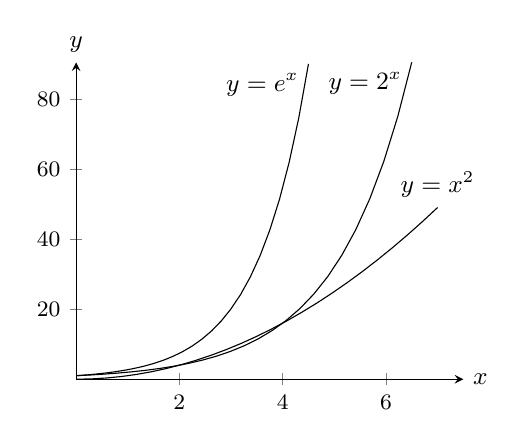
\begin{tikzpicture}[font=\small]
\begin{axis}[clip=false,small,axis lines=middle,xmin=0,ymin=0,xlabel={$x$},ylabel={$y$},xlabel style={at={(current axis.right of origin)},anchor=west},ylabel style={at={(current axis.above origin)},anchor=south},xmax=7.5]
\addplot[domain=0:4.5]{e^x}node[below left]{$y=e^x$};
\addplot[domain=0:6.5]{2^x}node[below left]{$y=2^x$};
\addplot[domain=0:7]{x^2}node[above]{$y=x^2$};
\end{axis}
\end{tikzpicture}
\caption{
تفاعل \عددی{y=e^x}، \عددی{y=2^x} اور تفاعل \عددی{y=x^2}
}
\label{شکل_ماورائی_قوت_نما_اور_دیگر_تفاعل}
\end{minipage}\hfill
\begin{minipage}{0.45\textwidth}
\centering
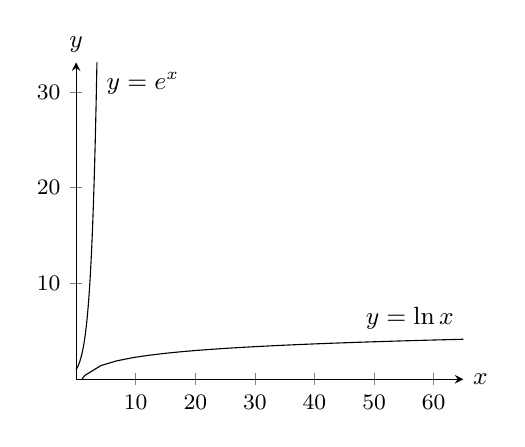
\begin{tikzpicture}[font=\small]
\begin{axis}[clip=false,small,axis lines=middle,xmin=0,ymin=0,xlabel={$x$},ylabel={$y$},xlabel style={at={(current axis.right of origin)},anchor=west},ylabel style={at={(current axis.above origin)},anchor=south}]
\addplot[domain=0:3.5]{e^x}node[below right]{$y=e^x$};
\addplot[domain=1:1.5]{ln(x)};
\addplot[domain=1.5:65]{ln(x)}node[above left]{$y=\ln x$};
\end{axis}
\end{tikzpicture}
\caption{
تفاعل \عددی{y=e^x} اور \عددی{y=\ln x} کا موازنہ
}
\label{شکل_ماورائی_قوت_نما_اور_لوگارتھمی_تفاعل}
\end{minipage}
\end{figure}

متغیر \عددی{x} بڑھاتے ہوئے تفاعل \عددی{y=e^x} کے بڑھنے کی شرح کو سمجھنے کی خاطر تصور کریں کہ آپ اس تفاعل کو ترسیم کرتے ہیں جہاں محور کا پیمانہ  \عددی{\SI{1}{\centi\meter}} ہے۔یوں \عددی{x=\SI{1}{\centi\meter}} پر \عددی{y=e^1\approx \SI{3}{\centi\meter}} ہو گا۔ یوں \عددی{x=\SI{6}{\centi\meter}} پر \عددی{y=e^6\approx\SI{403}{\centi\meter}} یعنی تقریباً \عددی{4} میٹر ہو گا جو کمرے کی چھت کے برابر ہو گا۔اسی طرح \عددی{x=\SI{10}{\centi\meter}} پر
 \عددی{y=e^{10}\approx \SI{22026}{\centi\meter}} یعنی \عددی{\SI{220}{\meter}} ہو گا جو شہر کے عموماً عمارتوں سے زیادہ بلند ہو گا۔ اگر \عددی{x=\SI{24}{\centi\meter}} ہو تب \عددی{y} چاند تک آدھے فاصلہ سے زیادہ طے کر چکا ہو گا اور \عددی{x=\SI{24}{\centi\meter}} پر \عددی{y} سورج کے قریب ترین ستارہ سے زیادہ دور ہو گا:
\begin{align*}
e^{43}&\approx \SI{4.73e18}{\centi\meter}\\
&=\SI{4.73e13}{\kilo\meter}\\
&\approx \text{\RL{$5$ نوری سال}}
\end{align*} 
اس کے باوجود \عددی{x} محور پر آپ مبدا سے صرف \عددی{\SI{43}{\centi\meter}} فاصلہ پر ہوں گے۔

اس کے برعکس \عددی{x\to\infty} کرنے سے لوگارتھمی تفاعل \عددی{y=\log_2x} اور \عددی{y=\ln x} کے بڑھنے کی شرح \عددی{x} کے کسی بھی مثبت طاقت کے بڑھنے کی شرح سے کم ہو گی (سوال \حوالہ{سوال_ماورائی_لوگارتھم_سب_سے_آہستہ})۔یوں محور کا پیمانہ \عددی{\SI{1}{\centi\meter}} لیتے ہوئے مبدا سے صرف \عددی{\SI{43}{\centi\meter}} بلندی تک پہنچنے کی خاطر آپ کو محور \عددی{x} پر \عددی{5} نوری سال دور جانا ہو گا (شکل \حوالہ{شکل_ماورائی_قوت_نما_اور_لوگارتھمی_تفاعل})۔

قوت نما، کثیر رکنی اور لوگارتھمی تفاعل کا ایک دوسرے کے ساتھ مذکورہ بالا موازنہ کو زیادہ درستگی سے بیان کرنے کی خاطر ہم ایک تعریف پیش کرتے ہیں۔جب ہم کہتے ہیں کہ \عددی{x\to \infty} کرنے سے کسی بھی تفاعل \عددی{g(x)} کے بڑھنے کی شرح سے  تفاعل \عددی{f(x)} کے بڑھنے کی شرح زیادہ ہے تب اس سے مراد درج ذیل ہو گا۔

\ابتدا{تعریف}\موٹا{\عددی{x\to \infty} کرتے ہوئے بڑھنے کی شرح}\\
فرض کریں کافی بڑے \عددی{x} کے لئے \عددی{f(x)} اور \عددی{g(x)} مثبت ہیں۔
\begin{enumerate}[a.]
\item
اگر 
\begin{align*}
\lim_{x\to\infty}\frac{f(x)}{g(x)}=\infty
\end{align*}
یا، اس کا مماثل
\begin{align*}
\lim_{x\to\infty}\frac{g(x)}{f(x)}=0
\end{align*}

ہو تب  \عددی{x\to\infty} کرتے ہوئے \عددی{f} کے بڑھنے کی شرح، \عددی{g} کے بڑھنے کی شرح سے زیادہ ہو گی۔ ہم یہ بھی کہہ سکتے ہیں کہ \عددی{x\to\infty} کرتے ہوئے \عددی{g} کے بڑھنے کی شرح، \عددی{f} کے بڑھنے کی شرح سے کم ہو گی۔
\item
اگر
\begin{align*}
\lim_{x\to\infty}\frac{f(x)}{g(x)}&=L=\ne 0&&\text{\RL{$L$ غیر صفر اور متناہی ہے}}
\end{align*}
ہو تب \عددی{x\to \infty} کرتے ہوئے \عددی{f} کے بڑھنے کی شرح،  \عددی{g} کے بڑھنے کی شرح کے برابر ہو گی۔
\end{enumerate}
\انتہا{تعریف}
%====================

ان تعریف کے تحت  تفاعل \عددی{y=2x} تفاعل \عددی{y=x} سے زیادہ تیزی سے نہیں بڑھتا ہے۔ اس کی وجہ 
\begin{align*}
\lim_{x\to\infty}\frac{2x}{x}=\lim_{x\to \infty}2=2
\end{align*}
ہے  جو غیر صفر اور متناہی حد ہے۔ زیادہ تیزی سے بڑھنے کے عمومی مطلب کو ہم اس لئے نظر انداز  کرتے ہیں کہ جب ہم کہیں کہ \عددی{x} کی بڑی قیمتوں کے لئے \عددی{f} کے بڑھنے کی شرح \عددی{g} کے بڑھنے کی شرح سے زیادہ ہے تب اس سے مراد "\عددی{x} کی بڑی قیمتوں کے لئے \عددی{f} کے لحاظ سے \عددی{g} کی قیمت قابل نظر انداز ہے،" لینا چاہیے۔

\ابتدا{مثال}
\عددی{x\to\infty} کرتے ہوئے \عددی{x^2} کے لحاظ سے \عددی{e^x} درج ذیل کی بنا زیادہ تیزی سے بڑھتا ہے۔
\begin{align*}
\underbrace{\lim_{x\to\infty}\frac{e^x}{x^2}}_{\tfrac{\infty}{\infty}}&=
\underbrace{\lim_{x\to\infty}\frac{e^x}{2x}}_{\tfrac{\infty}{\infty}}=\lim_{x\to\infty}\frac{e^x}{2}=\infty
&&\text{\RL{قاعدہ لھوپیٹال دو مرتبہ استعمال کیا گیا}}
\end{align*}
\انتہا{مثال}
%===================
\ابتدا{مثال}
(ا) \عددی{x\to \infty} کرتے ہوئے \عددی{2^x} کے لحاظ سے \عددی{3^x} زیادہ تیزی سے بڑھتا ہے چونکہ:
\begin{align*}
\lim_{x\to \infty}\frac{3^x}{2^x}=\lim_{x\to \infty}\big(\frac{3}{2}\big)^x=\infty
\end{align*}
(ب) \عددی{x\to\infty} کرتے ہوئے مختلف اساس کے قوت نما تفاعل کبھی بھی ایک شرح شے نہیں بڑھتے ہیں۔اگر \عددی{a>b>0} ہو تب \عددی{a^x} کے بڑھنے کی شرح \عددی{b^x} کے بڑھنے کی شرح سے زیادہ ہو گی۔
\begin{align*}
\lim_{x\to\infty}\frac{a^x}{b^x}=\lim_{x\to\infty}\big(\frac{a}{b}\big)^x=\infty
\end{align*}
\انتہا{مثال}
%=============
\ابتدا{مثال}
\عددی{x\to\infty} کرتے ہوئے \عددی{x^2} کے بڑھنے کی شرح \عددی{\ln x} کے بڑھنے کی شرح سے زیادہ ہو گی:
\begin{align*}
\lim_{x\to\infty}\frac{2^x}{\ln x}=\lim_{x\to \infty}\frac{2x}{1/x}=\lim_{x\to\infty}2x^2=\infty
\end{align*}
\انتہا{مثال}
%================
\ابتدا{مثال}
\عددی{x\to\infty} کرنے سے \عددی{\ln x} کے بڑھنے کی شرح \عددی{x} کے بڑھنے کی شرح سے کم ہو گی:
\begin{align*}
\lim{x\to\infty}\frac{\ln x}{x}=\lim_{x\to \infty}\frac{1/x}{1}=\lim_{x\to\infty}\frac{1}{x}=0
\end{align*} 
\انتہا{مثال}
%================
\ابتدا{مثال}
قوت نما تفاعل کے برعکس \عددی{x\to\infty} کرتے ہوئے مختلف اساس کے لوگارتھمی تفاعل ایک جیسے شرح سے بڑھتے  ہیں:
\begin{align*}
\lim{x\to\infty}\frac{\log_a x}{\log_b x}=\lim_{x\to\infty}\frac{\ln x/\ln a}{\ln x/\ln b}=\frac{\ln b}{\ln a}
\end{align*} 
یہ حد غیر صفر اور متناہی ہے۔
\انتہا{مثال}
%======================

اگر \عددی{x\to\infty} کرتے ہوئے \عددی{f} کے بڑھنے کی شرح اور \عددی{g} کے بڑھنے کی شرح ایک دوسرے کے برابر ہو، اور \عددی{x\to\infty} کرتے ہوئے \عددی{gf} کے بڑھنے کی شرح اور \عددی{h} کے بڑھنے کی شرح ایک دوسرے کے برابر ہو، تب \عددی{x\to \infty} کرتے ہوئے \عددی{f} اور \عددی{h} کے بڑھنے کی شرح ایک دوسرے کے برابر ہو گی۔ اس کی وجہ
\begin{align*}
\lim_{x\to \infty}\frac{f}{g}=L_1\quad \text{اور}\quad \lim_{x\to\infty}\frac{g}{h}=L_2
\end{align*}
یعنی
\begin{align*}
\lim_{x\to\infty}\frac{f}{h}=\lim_{x\to\infty}\frac{f}{g}\cdot\frac{g}{h}=L_1L_2
\end{align*}
ہے۔اگر \عددی{L_1} اور \عددی{L_2} غیر صفر اور متناہی ہوں تب \عددی{L_1L_2} بھی غیر صفر اور متناہی ہو گا۔

\ابتدا{مثال}
دکھائیں کہ \عددی{x\to\infty} کرتے ہوئے \عددی{\sqrt{x^2+5}} اور \عددی{(2\sqrt{x}-1)^2} کے بڑھنے کی شرح ایک دوسرے جتنی ہے۔

حل:\quad
ہم دکھاتے ہیں کہ دونوں تفاعل کے بڑھنے کی شرح رہی ہے جو تفاعل \عددی{x} کی ہے:
\begin{align*}
\lim_{x\to\infty}\frac{\sqrt{x+5}}{x}&=\lim_{x\to\infty}\sqrt{1+\frac{5}{x^2}}=1\\
\lim_{x\to\infty}\frac{(2\sqrt{x}-1)^2}{x}&=\lim_{x\to \infty}\big(\frac{2\sqrt{x}-1}{\sqrt{x}}\big)^2=\lim_{x\to\infty}\big(2-\frac{1}{\sqrt{x}}\big)^2=4
\end{align*}
یوں دونوں تفاعل کے بڑھنے کی شرح ایک دوسرے جتنے ہو گی۔
\انتہا{مثال}
%=======================

\جزوحصہء{رتبہ اور "o" علامتیت}
بڑے \عددی{O} اور چھوٹے \عددی{o} کی علامت کمپیوٹر سائنس میں عام استعمال ہوتی ہے۔ انہیں یہاں متعارف کیا جاتا ہے۔

\ابتدا{تعریف}
اگر \عددی{   x\to\infty} کرتے ہوئے \عددی{\lim_{x\to \infty}\frac{f(x)}{g(x)}=0} ہو تب  ہم کہتے ہیں کہ \عددی{f} کا رتبہ \عددی{g} سے کم ہے جس کو \عددی{f=o(g)}  سے ظاہر کیا جاتا ہے۔ اس کو "\عددی{f}، \عددی{g} کا چھوٹا عددی{o} ہے" پڑھا جاتا ہے۔ 
\انتہا{تعریف}
%===================

یوں \عددی{x\to \infty} کرتے ہوئے \عددی{f=o(g)}  سے مراد \عددی{x\to \infty} کرتے ہوئے \عددی{f} کے بڑھنے کی شرح \عددی{g} سے کم ہے۔

\ابتدا{مثال}
\begin{align*}
\ln x&=o(x) \quad \text{پر}\quad x\to\infty\quad \text{لہٰذا}\quad \lim_{x\to\infty}\frac{\ln x}{x}=0\quad \text{چونکہ}\\
x^2&=o(x^3+1) \quad \text{پر}\quad x\to\infty\quad \text{لہٰذا}\quad \lim_{x\to\infty}\frac{x^2}{x^3+1}=0\quad \text{چونکہ}
\end{align*}
\انتہا{مثال}
%===================
\ابتدا{تعریف}
فرض کریں کافی بڑے \عددی{x} پر \عددی{f(x)} اور \عددی{g(x)} مثبت ہیں۔ تب کافی بڑے  \عددی{x} پر اگر کسی مثبت عدد صحیح \عددی{M} کے لئے
\begin{align*}
\frac{f(x)}{g(x)}\le M
\end{align*}
ہو تب \عددی{x\to\infty} پر \عددی{f} کا رتبہ زیادہ سے زیادہ \عددی{g} کے رتبے جتنا ہو گا۔ اس کو ہم \عددی{f=O(g)} سے ظاہر کرتے ہیں جس
 کو "\عددی{f}، \عددی{g} کا بڑا \عددی{O} ہے' پڑھا جاتا ہے۔
\انتہا{تعریف}
%=====================

\ابتدا{مثال}
چونکہ کافی بڑے \عددی{x} کے لئے \عددی{\frac{x+\sin x}{x}\le 2} ہے لہٰذا \عددی{x\to \infty} پر \عددی{x+\sin x=O(x)} ہو گا۔
\انتہا{مثال}
%=====================
\ابتدا{مثال}
\عددی{x\to\infty} پر \عددی{\frac{e^x+x^2}{e^x}\to 1}  کی بنا \عددی{x\to\infty} پر \عددی{e^x+x^2=O(e^x)} ہو گا۔ اسی طرح 
\عددی{x\to\infty} پر \عددی{\frac{x}{e^x}\to 0}  کی بنا \عددی{x\to\infty} پر \عددی{x=O(e^x)} ہو گا۔
\انتہا{مثال}
%=====================

تعریف پر دوبارہ نظر دوڑاتے ہوئے  آپ دیکھیں گے کہ کافی بڑے \عددی{x} پر مثبت تفاعل کے لئے  \عددی{f=o(g)}سے مراد \عددی{f=O(g)} ہے۔ اس کے علاوہ اگر \عددی{f} اور \عددی{g}  کے بڑھنے کی شرح ایک دوسرے جتنی ہو تب \عددی{f=O(g)} اور \عددی{g=O(f)} ہوں گے (سوال \حوالہ{سوال_ماورائی_ایک_برابر_شرح})۔ 

\جزوحصہ{ترتیبی اور ثنائی تلاش}
کمپیوٹر کسی لائحہ کار کے تحت قدم با قدم چل کر کوئی کام سر انجام دیتا ہے۔اس لائحہ کار کو \اصطلاح{کمپیوٹر الخوارزم}\فرہنگ{الخوارزم!کمپیوٹر}\حاشیہب{computer algorithm}\فرہنگ{algorithm} کہتے ہیں۔اس لائحہ کار کی کارگزاری جاننے کی خاطر ماہرین عموماً اس کام کو سرانجام کرنے کے کئے درکار قدموں کی گنتی کرتے ہیں۔ ایک ہی کام سرانجام دینے کے دو مختلف لائحہ کار کی کارگزاری میں بہت زیادہ فرق ہو سکتا ہے جنہیں بڑے \عددی{O} علامتی روپ میں پیش کیا جاتا ہے۔ آئیں ایک مثال دیکھتے ہیں۔

ایک لغت میں کسی ایک حرف سے شروع ہونے والے الفاظ کی تعداد  \عددی{\num{26000}} ہے۔ آپ اس حرف سے شروع ہونے والے ایک لفظ کو دو طریقوں سے تلاش کر سکتے ہیں۔ پہلی ترکیب میں آپ پہلے لفظ سے شروع کرتے ہوئے ایک ایک لفظ پڑھ کر درکار لفظ تک پہنچتے ہیں۔ اس ترکیب کو \اصطلاح{ترتیبی تلاش}\فرہنگ{تلاش!ترتیبی}\حاشیہب{sequential search}\فرہنگ{search!sequential} کہتے ہیں جو لغت میں ترتیب سے الفاظ لکھے گئے ہونے سے استفادہ نہیں کرتا ہے۔ اس ترتیب میں آپ ہر صورت لفظ تلاش کر پائیں گے (یا جان جائیں گے کہ یہ لفظ لغت میں موجود نہیں ہے) لیکن عین ممکن ہے کہ آپ کو \عددی{\num{26000}} قدم چلنا پڑے۔

اس سے بہتر ترکیب میں آپ لغت کے عین وسط (ایک دو الفاظ آگے پیچھے ہو سکتے ہیں) میں ایک لفظ کو دیکھتے ہیں۔ چونکہ لغت میں الفاظ ترتیب سے ہیں لہٰذا آپ معلوم کر پائیں گے کہ آیا درکار لفظ پہلی نصف یا دوسری نصف حصہ میں ہے۔ لغت کی اس نصف حصہ کو رد کریں جس میں لفظ موجود نہیں ہے۔یوں پہلی قدم میں \عددی{\num{13000}} الفاظ سے چھٹکارا حاصل ہوتا ہے۔  اب منتخب حصہ کے نصف میں جا کر دیکھیں کہ درکار لفظ کس جانب پایا جاتا ہے۔ یوں دوسرے قدم میں \عددی{6500} الفاظ سے چھٹکارا حاصل ہوتا ہے۔ اسی طرح ہر قدم پر آدھے حصے کو رد کرتے ہوئے چلتے جائیں جب تک آپ درکار لفظ تلاش نہیں کر پاتے یا الفاظ ختم نہیں ہو جاتے۔ چونکہ
\begin{align*}
\frac{26000}{2^{15}}<1
\end{align*}
ہوتا ہے لہٰذا  آپ کو زیادہ سے زیادہ \عددی{15} قدم چل کر درکار لفظ مل جائے گا یا آپ جان جائیں گے کہ یہ لفظ لغت میں موجود نہیں ہے۔ اس ترتیب کو \اصطلاح{ثنائی!تلاش}\فرہنگ{ثنائی تلاش}\حاشیہب{binary search}\فرہنگ{search!binary} کہتے ہیں۔

ایک سلسلہ جس کی لمبائی \عددی{n} ہو میں کسی جزو کی تلاش کے لئے ترتیبی تلاش کو \عددی{n} قدم درکار ہو سکتے ہیں۔ اس کے برعکس ثنائی تلاش استعمال کرتے ہوئے  اگر \عددی{2^{m-1}<n<2^m} ہو تب \عددی{m-1<\log_2n\le m} ہو گا اور ایک لفظ تک پہنچنے کی خاطر زیادہ سے زیادہ \عددی{m=\lceil\log_2n\rceil} (\عددی{\log_2n} کا عدد صحیح چھت تفاعل)  بار دو حصوں میں تقسیم کی ضرورت پیش آئے گی۔ یوں ثنائی تلاش میں  \عددی{\log_2 n} کے لگ بھگ  قدم درکار ہوں گے۔ 

بڑے \عددی{O} روپ میں اس تمام کو نہایت خوش اسلوبی سے ظاہر کیا جا سکتا ہے۔ ترتیبی سلسلہ میں ترتیبی تلاش کو \عددی{O(n)} کے لگ بھگ قدم درکار ہوں گے جبکہ ثنائی تلاش کو \عددی{O(\log_2n)} کے لگ بھگ قدم درکار ہوں گے۔ ہماری مثال میں ان دو میں بہت زیادہ فرق پایا جاتا ہے (\عددی{\num{26000}} بالمقابل \عددی{15}) اور چونکہ \عددی{n\to \infty} کرتے ہوئے \عددی{\log_2n} کے لحاظ سے \عددی{n} زیادہ تیزی سے بڑھتا ہے لہٰذا \عددی{n} بڑھانے سے یہ فرق زیادہ بڑھے گا۔


\حصہء{سوالات}
\موٹا{قوت نما \عددی{e^x} کے ساتھ موازنہ}

\ابتدا{سوال}
\عددی{x\to\infty} کرتے ہوئے درج ذیل میں سے کونسا تفاعل \عددی{e^x} سے زیادہ تیزی سے بڑھتا ہے؟ کونسا \عددی{e^x} کی شرح سے بڑھتا ہے؟  کونسا \عددی{e^x} سے کم تیزی سے بڑھتا ہے؟
\begin{multicols}{4}
\begin{enumerate}[a.]
\item
$x+3$
\item
$x^3+\sin^2x$
\item
$\sqrt{x}$
\item
$4^x$
\item
$(\tfrac{3}{2})^x$
\item
$e^{x/2}$
\item
$\frac{e^x}{2}$
\item
$\log_{10}x$
\end{enumerate}
\end{multicols}
جواب:\quad
(ا) آہستہ (ب) آہستہ (ج) آہستہ (د) تیز (ہ) آہستہ  (و) آہستہ (ز) ایک جیسا (ح) آہستہ
\انتہا{سوال}
%======================
\ابتدا{سوال}
\عددی{x\to\infty} کرتے ہوئے درج ذیل میں سے کونسا تفاعل \عددی{e^x} سے زیادہ تیزی سے بڑھتا ہے؟ کونسا \عددی{e^x} کی شرح سے بڑھتا ہے؟  کونسا \عددی{e^x} سے کم تیزی سے بڑھتا ہے؟
\begin{multicols}{4}
\begin{enumerate}[a.]
\item
$10x^4+30x+1$
\item
$x\ln x-x$
\item
$\sqrt{1+x^4}$
\item
$(\tfrac{5}{2})^x$
\item
$e^{-x}$
\item
$xe^x$
\item
$e^{\cos x}$
\item
$e^{x-1}$
\end{enumerate}
\end{multicols}
\انتہا{سوال}
%======================
\موٹا{طاقت \عددی{x^2} کے ساتھ موازنہ}

\ابتدا{سوال}
\عددی{x\to\infty} کرتے ہوئے درج ذیل میں سے کونسا تفاعل \عددی{x^2} سے زیادہ تیزی سے بڑھتا ہے؟ کونسا \عددی{x^2} کی شرح سے بڑھتا ہے؟  کونسا \عددی{x^2} سے کم تیزی سے بڑھتا ہے؟
\begin{multicols}{4}
\begin{enumerate}[a.]
\item
$x^2+4x$
\item
$x^5-x^2$
\item
$\sqrt{x^4+x^3}$
\item
$(x+3)^2$
\item
$x\ln x$
\item
$2^x$
\item
$x^3e^{-x}$
\item
$8x^2$
\end{enumerate}
\end{multicols}
جواب:\quad
(ا) ایک جیسا (ب) تیز (ج) ایک جیسا (د) ایک جیسا (ہ) آہستہ (و) تیز (ز) آہستہ (ح) ایک جیسا 
\انتہا{سوال}
%======================
\ابتدا{سوال}
\عددی{x\to\infty} کرتے ہوئے درج ذیل میں سے کونسا تفاعل \عددی{x^2} سے زیادہ تیزی سے بڑھتا ہے؟ کونسا \عددی{x^2} کی شرح سے بڑھتا ہے؟  کونسا \عددی{x^2} سے کم تیزی سے بڑھتا ہے؟
\begin{multicols}{4}
\begin{enumerate}[a.]
\item
$x^2+\sqrt{x}$
\item
$10x^2$
\item
$x^2e^{-x}$
\item
$\log_{10}(x^2)$
\item
$x^3-x^2$
\item
$(\tfrac{1}{10})^x$
\item
$(1.1)^x$
\item
$x^2+100x$
\end{enumerate}
\end{multicols}
\انتہا{سوال}
%======================
\موٹا{لوگارتھم \عددی{\ln x} کے ساتھ موازنہ}

\ابتدا{سوال}
\عددی{x\to\infty} کرتے ہوئے درج ذیل میں سے کونسا تفاعل \عددی{\ln x} سے زیادہ تیزی سے بڑھتا ہے؟ کونسا \عددی{\ln x} کی شرح سے بڑھتا ہے؟  کونسا \عددی{\ln x} سے کم تیزی سے بڑھتا ہے؟
\begin{multicols}{4}
\begin{enumerate}[a.]
\item
$\log_3x$
\item
$\ln 2x$
\item
$\ln \sqrt{x}$
\item
$\sqrt{x}$
\item
$x$
\item
$5\ln x$
\item
$\frac{1}{x}$
\item
$e^x$
\end{enumerate}
\end{multicols}
جواب:\quad
(ا) ایک جیسا (ب) ایک جیسا (ج) ایک جیسا (د) تیز (ہ) تیز (و) ایک جیسا (ز) آہستہ (ح) تیز 
\انتہا{سوال}
%======================
\ابتدا{سوال}
\عددی{x\to\infty} کرتے ہوئے درج ذیل میں سے کونسا تفاعل \عددی{\ln x} سے زیادہ تیزی سے بڑھتا ہے؟ کونسا \عددی{\ln x} کی شرح سے بڑھتا ہے؟  کونسا \عددی{\ln x} سے کم تیزی سے بڑھتا ہے؟
\begin{multicols}{4}
\begin{enumerate}[a.]
\item
$\log_2(x^2)$
\item
$\log_{10}10x$
\item
$\frac{1}{\sqrt{x}}$
\item
$\frac{1}{x^2}$
\item
$x-2\ln x$
\item
$e^{-x}$
\item
$\ln(\ln x)$
\item
$\ln(2x+5)$
\end{enumerate}
\end{multicols}
\انتہا{سوال}
%======================
\موٹا{شرح نمو کے لحاظ سے منظم کرنا}

\ابتدا{سوال}
\عددی{x\to \infty} کرتے ہوئے شرح نمو کے لحاظ سے منظم کریں۔ کم تر شرح والے تفاعل کو پہلے لکھیں۔ 
\begin{multicols}{4}
\begin{enumerate}[a.]
\item
$e^x$
\item
$x^x$
\item
$(\ln x)^x$
\item
$e^{x/2}$
\end{enumerate}
\end{multicols}
جواب:\quad
د، ا، ج، ب
\انتہا{سوال}
%====================
\ابتدا{سوال}
\عددی{x\to \infty} کرتے ہوئے شرح نمو کے لحاظ سے ترتیب دیں۔ کم تر شرح والے تفاعل کو پہلے لکھیں۔ 
\begin{multicols}{4}
\begin{enumerate}[a.]
\item
$2^x$
\item
$x^2$
\item
$(\ln 2)^x$
\item
$e^x$
\end{enumerate}
\end{multicols}
\انتہا{سوال}
%====================
\موٹا{بڑا \عددی{O} اور چھوٹا \عددی{o}؛ رتبہ}

\ابتدا{سوال}
\عددی{x\to\infty} کرتے ہوئے کونسا درست اور کونسا غلط ہے؟
\begin{multicols}{3}
\begin{enumerate}[a.]
\item
$x=o(x)$
\item
$x=o(x+5)$
\item
$x=O(x+5)$
\item
$x=O(2x)$
\item
$e^x=o(e^{2x})$
\item
$x+\ln x=O(x)$
\item
$\ln x=o(\ln 2x)$
\item
$\sqrt{x^2+5}=O(x)$
\end{enumerate}
\end{multicols}
جواب:\quad
(ا) غلط (ب) غلط (ج) درست (د) درست (ہ) درست (و) درست (ز) غلط (ح) درست
\انتہا{سوال}
%============
\ابتدا{سوال}
\عددی{x\to\infty} کرتے ہوئے کونسا درست اور کونسا غلط ہے؟
\begin{multicols}{3}
\begin{enumerate}[a.]
\item
$\frac{1}{x+3}=O(\tfrac{1}{x})$
\item
$\frac{1}{x}+\frac{1}{x^2}=O(\tfrac{1}{x})$
\item
$\frac{1}{x}-\frac{1}{x^2}=o(\tfrac{1}{x})$
\item
$2+\cos x=O(2)$
\item
$e^x+x=O(e^x)$
\item
$x\ln x=o(x^2)$
\item
$\ln(\ln x)=O(\ln x)$
\item
$\ln x=o(\ln(x^2+1))$
\end{enumerate}
\end{multicols}
\انتہا{سوال}
%============
\ابتدا{سوال}\شناخت{سوال_ماورائی_ایک_برابر_شرح}
دکھائیں کہ اگر \عددی{x\to\infty} کرنے سے \عددی{f(x)} اور \عددی{g(x)} کے بڑھنے کی شرح برابر ہو تب \عددی{f=O(g)} اور \عددی{g=O(f)} ہوں گے۔
\انتہا{سوال}
%======================
\ابتدا{سوال}
\عددی{x\to \infty} کرتے ہوئے کب کثیر رکنی \عددی{f(x)} کا رتبہ کثیر رکنی \عددی{g(x)} کے رتبہ سے کم ہو گا؟ اپنے جواب کی وجہ پیش کریں۔
\انتہا{سوال}
%===================
\ابتدا{سوال}
\عددی{x\to \infty} کرتے ہوئے کب کثیر رکنی \عددی{f(x)} کا رتبہ زیادہ سے زیادہ کثیر رکنی \عددی{g(x)} کے رتبہ کے برابر ہو گا؟ اپنے جواب کی وجہ پیش
 کریں۔\\
جواب:\quad
جب \عددی{f} کا درجہ \عددی{g} کے درجہ سے کم یا اس کے برابر ہو۔
\انتہا{سوال}
%=====================
\ابتدا{سوال}\ترچھا{قاعدہ سمسن اور قاعدہ ذوزنقہ}\\
موجودہ حصہ میں پیش کی گئی تعریف کو زیادہ عمومی بنانے کی خاطر ہم اس میں \عددی{x\to\infty} کی پابندی ختم کر کے اس  کی بجائے \عددی{x\to a} پر حد لیتے ہیں جہاں \عددی{a} حقیقی عدد ہے۔ دکھائیں کہ قاعدہ سمسن سے حاصل قطعی تکمل کی تخمین میں \عددی{h\to 0} کرتے ہوئے خلل \عددی{O(h^4)} ہو گا جبکہ قاعدہ ذوزنقہ سے حاصل تخمین میں خلل \عددی{O(h^2)} ہو گا۔ یوں ان دو تراکیب کے نتائج کی درستگی کو اس طرح بھی بیان کیا جا سکتا ہے۔  
\انتہا{سوال}
%===================
\موٹا{دیگر موازنے}

\ابتدا{سوال}
ناطق تفاعل کے حد کے بارے میں حصہ \حوالہ{حصہ_استعمال_تفرق_حد_متقارب_اور_غالب_اجزاء} میں حاصل نتیجہ ہمیں \عددی{x\to \infty} کی صورت میں کثیر رکنی کی اضافی  شرح نمو کے بارے میں کیا بتاتا ہے؟\\
جواب:\quad
زیادہ درجے کا کثیر رکنی، کم درجے کے کثیر رکنی سے زیادہ تیز بڑھتا ہے۔ ایک جیسے درجہ کے کثیر رکنی کی شرح نمو برابر ہوتی ہے۔
\انتہا{سوال}
%=======================
\ابتدا{سوال}\ترچھا{کمپیوٹر ترسیم}\\
(ا) درج ذیل پر تحقیق کریں۔ اس کے بعد قاعدہ لھوپیٹال سے اس تحقیق سے حاصل معلومات کی وجہ بیان کریں۔
\begin{align*}
\lim_{x\to\infty}\frac{\ln(x+1)}{\ln x},\quad \lim_{x\to \infty}\frac{\ln(x+999)}{\ln x}
\end{align*}
(ب) دکھائیں کہ درج ذیل کی قیمت ، مستقل\عددی{a} کی قیمت پر منحصر نہیں ہے۔ اس سے تفاعل \عددی{f(x)=\ln(x+a)} اور \عددی{g(x)=\ln x} کے اضافی شرح نمو کے بارے میں کیا کہا جا سکتا ہے؟
\begin{align*}
\lim_{x\to\infty}\frac{\ln(x+a)}{\ln x}
\end{align*}
\انتہا{سوال}
%=============================
\ابتدا{سوال}
دکھائیں کہ \عددی{x\to \infty} کرتے ہوئے \عددی{\sqrt{10x+1}} اور \عددی{\sqrt{x+1}} کی شرح نمو ایک دوسرے کے برابر ہیں۔ یہ دکھانے کی خاطر دکھائیں کہ دونوں تفاعل کی شرح نمو تفاعل \عددی{\sqrt{x}} کے شرح نمو کے برابر ہے۔ 
\انتہا{سوال}
%====================
\ابتدا{سوال}
دکھائیں کہ \عددی{x\to \infty} کرتے ہوئے \عددی{\sqrt{x^4+x}} اور \عددی{\sqrt{x^4-x^3}} کی شرح نمو ایک دوسرے کے برابر ہیں۔ یہ دکھانے کی خاطر دکھائیں کہ دونوں تفاعل کی شرح نمو تفاعل \عددی{x^2} کے شرح نمو کے برابر ہے۔ 
\انتہا{سوال}
%====================
\ابتدا{سوال}\شناخت{سوال_ماورائی_قوت_نمائی_کثیر_رکنی_سے_تیز}
دکھائیں کہ \عددی{x\to \infty} کرتے ہوئے \عددی{e^x} کی شرح نمو کسی بھی \عددی{x^n} کے شرح نمو سے زیادہ ہو گی، جہاں \عددی{n} کوئی بھی مثبت عدد صحیح ہو سکتا ہے، مثلاً \عددی{x^{\num{1000000}}}۔ (اشارہ۔ \عددی{x^n} کا \عددی{n} واں تفرق کیا ہے؟)
\انتہا{سوال}
%=================
\ابتدا{سوال}\ترچھا{تفاعل \عددی{e^x} ہر کثیر رکنی سے زیادہ تیزی سے بڑھتا ہے}\\
دکھائیں کہ \عددی{x\to\infty} کرتے ہوئے \عددی{e^x} کسی بھی کثیر رکنی \عددی{a_nx^n+a_{n-1}x^{n-1}+\cdots+a_1x+a_0} سے زیادہ تیزی سے بڑھتا ہے۔
\انتہا{سوال}
%====================
\ابتدا{سوال}\شناخت{سوال_ماورائی_لوگارتھم_سب_سے_آہستہ}
\begin{enumerate}[a.]
\item
دکھائیں کہ کسی بھی مثبت عدد صحیح \عددی{n} کی صورت میں \عددی{x\to \infty} کرتے ہوئے \عددی{\ln x} کی شرح نمو تفاعل \عددی{x^{1/n}} (مثلاً \عددی{x^{1/\num{1000000}}}) کی شرح نمو سے کم ہو گی۔
\item
اگرچہ \عددی{x^{1/\num{1000000}}} کی قیمت آخر کار \عددی{\ln x} کی قیمت سے زیادہ ہو گی، وہاں تک پہنچنے کے لئے آپ کو محور \عددی{x} پر بہت دور جانا ہو گا۔ ایسا \عددی{x>1} تلاش کریں جس پر \عددی{x^{1/{\num{1000000}}}>\ln x} ہو۔ دھیان رہے کہ \عددی{x>1} کی صورت میں مساوات \عددی{\ln x=x^{1/\num{1000000}}} کو \عددی{\ln(\ln x)=\tfrac{\ln x}{\num{1000000}}} بھی لکھا جا سکتا ہے۔
\item
تفاعل \عددی{x^{1/10}} کو بھی \عددی{\ln x} سے بڑھنے  کے لئے  بہت وقت درکار ہو گا۔ کیلکولیٹر استعمال کرتے ہوئے \عددی{x} کی وہ قیمت تلاش کریں جس پر \عددی{x^{1/10}} کی ترسیم \عددی{\ln x} کی ترسیم کو کٹ کرتی ہو یا جہاں \عددی{\ln x=10\ln(\ln x)} ہو۔
\item
وہ نقطہ جس پر \عددی{\ln x=10\ln(\ln x)} ہو کے قریب اس مساوات  کو کمپیوٹر پر ترسیم کر کے \عددی{x} تلاش کریں۔
\end{enumerate}
جواب:\quad
(ب) 
$\ln(e^{\num{17000000}})=\num{17000000}<(e^{17\times 10^6})^{1/10^6}=e^{17}\approx \num{24154952.75}$\\
(ج)  \عددی{x\approx 3.4306311\times 10^{15}}، (د) نقطہ تقاطع \عددی{x\approx 3.4306311\times 10^{15}} ہے۔
\انتہا{سوال}
%===================
\ابتدا{سوال}\ترچھا{تفاعل \عددی{\ln x} کی شرح نمو ہر کثیر رکنی سے کم ہے}\\
دکھائیں کہ \عددی{x\to\infty} کرتے ہوئے \عددی{\ln x} کی شرح نمو کسی بھی غیر مستقل کثیر رکنی سے کم ہو گی۔
\انتہا{سوال}
%===================
\موٹا{الخوارزم اور تلاش}\\

\ابتدا{سوال}\شناخت{سوال_ماورائی_تلاش_کی_قدمیں}
(ا) آپ کمپیوٹر کی مدد سے ایک کام سرانجام دینا چاہتے ہیں۔ آپ کے پاس تین الخوارزم موجود ہیں جن  کے لئے کمپیوٹر کو درکار   قدموں کی تعداد  درج ذیل تفاعل دیتے ہیں۔ \عددی{n} کی بڑی قیمت کی صورت میں ان میں سے کونسا الخوارزم  بہترین ہے؟ اپنے جواب کی وجہ پیش کریں۔
\begin{align*}
n\log_2n,\quad n^{3/2},\quad n(\log_2n)^2
\end{align*}
(ب) جزو-الف میں دیے گئے تفاعل کو ایک ساتھ ترسیم کرتے ہوئے دیکھیں کونسا زیادہ تیزی سے بڑھتا ہے۔\\
جواب:\quad
(ا) جو \عددی{O(n\log_2n)} قدم چلتا ہے۔
\انتہا{سوال}
%====================
\ابتدا{سوال}
درج ذیل تفاعل کے لئے سوال \حوالہ{سوال_ماورائی_تلاش_کی_قدمیں} کو دہرائیں۔
\begin{align*}
n,\quad \sqrt{n}\log_2n,\quad (\log_2n)^n
\end{align*}
\انتہا{سوال}
%=====================
\ابتدا{سوال}
ایک مرتب سلسلہ جس میں دس لاکھ اجزاء پائے جاتے ہیں میں سے آپ کو ایک جزو تلاش کرنا ہے۔ ترتیبی تلاش کے لئے کتنے قدم درکار ہوں گے؟ ثنائی تلاش کے لئے کتنے قدم درکار ہوں گے؟\\
جواب:\quad
ترتیبی تلاش کو دس لاکھ قدم چلنا پڑھ سکتا ہے جبکہ ثنائی تلاش میں زیادہ سے زیادہ \عددی{20} قدم چلنا ہو گا۔
\انتہا{سوال}
%=================
\ابتدا{سوال}
ایک مرتب سلسلہ میں \عددی{\num{450000}} اجزاء پائے جاتے ہیں جن میں سے آپ کو ایک جزو کی تلاش ہے۔ ترتیبی تلاش اور ثنائی تلاش کرتے ہوئے کتنے قدم درکار ہوں گے؟
\انتہا{سوال}
%===================

\حصہ{الٹ تکونیاتی تفاعل}
الٹ تکونی تفاعل کی ضرورت اس وقت پیش آتی ہے جب ہم مثلث کے ضلع کو ناپ کر زاویہ تلاش کرنا چاہتے ہیں۔ یہ تفاعل اہم الٹ تفرق بھی مہیا کرتے ہیں اور تفرقی مساوات کے حل میں عموماً پائے جاتے ہیں۔ اس حصہ میں ان تفاعل کی تعریف پیش کی جائے گی، ان کو ترسیم کرنا سکھایا جائے گا اور ان کی قیمت حاصل کرنا سکھایا جائے گا۔

\جزوحصہء{الٹ تکونیاتی  کی تعریف}
چھ بنیادی تکونیاتی تفاعل کی قیمتیں دہراتی ہیں لہٰذا یہ ایک ایک تفاعل نہیں ہیں البتہ ان کے دائرہ کار کو ایسے وقفوں پر پابند کیا جا سکتا ہے جہاں یہ ایک ایک ہوں (جدول \حوالہ{جدول_ماورائی_تکونیاتی_تفاعل_ایک_ایک})۔
\begin{table}
\caption{تکونیاتی تفاعل کو ایک ایک بنانے کی خاطر دائرہ کار کو محدود کیا گیا ہے۔}
\label{جدول_ماورائی_تکونیاتی_تفاعل_ایک_ایک}
\centering
\renewcommand{\arraystretch}{2} 
\begin{tabular}{LLL}
\toprule
\text{تفاعل}&\text{\RL{دائرہ کار}}&\text{سعت}\\
\midrule
\sin x&[-\tfrac{\pi}{2},\tfrac{\pi}{2}]&[-1,1]\\
\cos x&[0,\pi]&[-1,1]\\
\tan x&(-\tfrac{\pi}{2},\tfrac{\pi}{2})&(-\infty,\infty)\\
\cot x&(0,\pi)&(-\infty,\infty)\\
\sec x&[0,\tfrac{\pi}{2})\cup (\tfrac{\pi}{2},\pi]&(-\infty,-1]\cup[1,\infty)\\
\csc x&[-\tfrac{\pi}{2},0)\cup(0,\tfrac{\pi}{2}]&(-\infty,-1]\cup[1,\infty)\\
\bottomrule
\end{tabular}
\end{table}

چونکہ محدود دائرہ کار والے تکونیاتی تفاعل ایک ایک ہیں لہٰذا ان کا الٹ پائے جاتے ہیں جنہیں ظاہر کرنا کا طریقہ درج ذیل ہے۔
\begin{align*}
y&=\sin^{-1}x\\
y&=\cos^{-1}x\\
y&=\tan^{-1}x\\
y&=\cot^{-1}x\\
y&=\sec^{-1}x\\
y&=\csc^{-1}x
\end{align*}
ہم کہیں گے "\عددی{x} کا الٹ سائن \عددی{y} کے برابر ہے"، وغیرہ۔ یاد رہے کہ ان الٹ تفاعل میں \عددی{-1} سے مراد الٹ تفاعل ہے اور لہٰذا اس کو ہرگز بالعکس متناسب تصور نہیں کیا جائے۔ مثال کے طور پر \عددی{\sin x} کا بالعکس متناسب \عددی{(\sin x)^{-1}=\tfrac{1}{\sin x}=\csc x} ہو گا۔

الٹ تکونیاتی تفاعل کے دائرہ کار یوں منتخب کئے جاتے ہیں کہ درج ذیل مطمئن ہوں۔
\begin{align}
\sec^{-1}x&=\cos^{-1}(\tfrac{1}{x})\label{مساوات_ماورائی_چند_تماثل_الف}\\
\csc^{-1}x&=\sin^{-1}(\tfrac{1}{x})\label{مساوات_ماورائی_چند_تماثل_ب}\\
\cot^{-1}x&=\tfrac{\pi}{2}-\tan^{-1}x \label{مساوات_ماورائی_چند_تماثل_ج}
\end{align}

ان تعلقات کو استعمال کر کے \عددی{\cos^{-1}x}، \عددی{\sin^{-1}x} اور \عددی{\tan^{-1}x} کی قیمتیں جانتے ہوئے ہم بالترتیب \عددی{\sec^{-1}x}، \عددی{\csc^{-1}x} اور \عددی{\cot^{-1}x} کی قیمتیں معلوم کر سکتے ہیں۔

\جزوحصہء{الٹ سائن اور الٹ کوسائن}
 متغیر \عددی{x} کے الٹ سائن یعنی \عددی{\sin^{-1}x} سے مراد وہ زاویہ ہے جس کا سائن \عددی{x} کے برابر ہو۔ اسی طرح \عددی{\cos^{-1}x} سے مراد وہ زاویہ ہے جس کے کوسائن کی قیمت \عددی{x} ہو۔

\ابتدا{تعریف}
\عددی{y=\sin^{-1}x} سے مراد وقفہ \عددی{[-\pi/2,\pi/2]} میں وہ عدد \عددی{y} ہے جس کے لئے \عددی{\sin y=x} ہو۔ اسی طرح 
\عددی{y=\cos^{-1}x} سے مراد وقفہ \عددی{[0,\pi]} میں وہ عدد \عددی{y} ہے جس کے لئے \عددی{\cos y=x} ہو۔
\انتہا{تعریف}
%=============

تفاعل \عددی{y=\sin^{-1}x} (شکل \حوالہ{شکل_ماورائی_سائن_اور_الٹ_سائن}) کی ترسیم مبدا کے لحاظ سے تشاکلی ہے (اور عین \عددی{x=\sin y} کی ترسیم پر پائی جاتی ہے)۔ یوں الٹ سائن طاق تفاعل ہے:
\begin{align}\label{مساوات_ماورائی_الٹ_سائن_تعلق}
\sin^{-1}(-x)=-\sin^{-1}x
\end{align}
تفاعل \عددی{y=\cos^{-1}x} (شکل \حوالہ{شکل_ماورائی_کوسائن_اور_الٹ_کوسائن}) کی ترسیم میں ایسی کوئی تشاکلی نہیں پائی جاتی ہے۔
\begin{figure}
\centering
\begin{subfigure}{0.45\textwidth}
\centering
\begin{tikzpicture}[font=\small,declare function={f(\x)=sin(deg(\x));}]
\pgfmathsetmacro{\k}{pi/2}
\begin{axis}[clip=false,small,axis lines=middle,xlabel={$x$},ylabel={$y$},xlabel style={at={(current axis.right of origin)},anchor=west},ylabel style={at={(current axis.above origin)},anchor=south},xtick={-\k,\k},xticklabels={$-\tfrac{\pi}{2}$,$\tfrac{\pi}{2}$},ytick={-1,1},enlargelimits=true]
\addplot[domain=-\k:\k,smooth]{f(x)};
\addplot[dashed,domain=-\k:-\k-1,smooth]{f(x)};
\addplot[dashed,domain=\k:\k+1,smooth]{f(x)};
\draw(-0.5,0.5)node[left,font=\scriptsize]{$\begin{aligned}y=\sin x,\, -\tfrac{\pi}{2}\le x\le \tfrac{\pi}{2}\\ [-\pi/2,\pi/2]\quad \text{\RL{دائرہ کار:}} \\ 
[-1,1] \quad \text{سعت:}   \end{aligned}$};
\draw(\k,{f(\k)})node[circ]{};
\draw(-\k,{f(-\k)})node[circ]{};
\end{axis}
\end{tikzpicture}
\caption{}
\end{subfigure}\hfill
\begin{subfigure}{0.45\textwidth}
\centering
\begin{tikzpicture}[font=\small,declare function={f(\x)=sin(deg(\x));}]
\pgfmathsetmacro{\k}{pi/2}
\begin{axis}[clip=false,small,axis lines=middle,xlabel={$x$},ylabel={$y$},xlabel style={at={(current axis.right of origin)},anchor=west},ylabel style={at={(current axis.above origin)},anchor=south},ytick={-\k,\k},yticklabels={$-\tfrac{\pi}{2}$,$\tfrac{\pi}{2}$},xtick={-1,1},enlargelimits=true]
\addplot[domain=-\k:\k,smooth]({f(x)},x);
\addplot[dashed,domain=-\k:-\k-1,smooth]({f(x)},x);
\addplot[dashed,domain=\k:\k+1,smooth]({f(x)},x)node[above]{$x=\sin y$};
\draw(-0.25,1.5)node[left,font=\scriptsize]{$\begin{aligned}y=\sin^{-1} x\\ [-1,1]\quad \text{\RL{دائرہ کار:}} \\ [-\pi/2,\pi/2]\quad \text{\RL{سعت:}} \end{aligned}$};
\draw({f(\k)},\k)node[circ]{};
\draw({f(-\k)},-\k)node[circ]{};
\end{axis}
\end{tikzpicture}
\caption{}
\end{subfigure}
\caption{
ترسیمات برائے (ا) \عددی{y=\sin x,\,-\pi/2\le x\le \pi/2}  اور (ب)  الٹ سائن تفاعل \عددی{y=\sin^{-1}x}؛ لکیر \عددی{y=x} میں عکس \عددی{\sin^{-1}x} درحقیقت قوس \عددی{x=\sin y} کا کچھ حصہ ہے۔
}
\label{شکل_ماورائی_سائن_اور_الٹ_سائن}
\end{figure}
%
\begin{figure}
\centering
\begin{subfigure}{0.45\textwidth}
\centering
\begin{tikzpicture}[font=\small,declare function={f(\x)=cos(deg(\x));}]
\pgfmathsetmacro{\k}{pi}
\pgfmathsetmacro{\kh}{pi/2}
\begin{axis}[clip=false,small,axis lines=middle,xlabel={$x$},ylabel={$y$},xlabel style={at={(current axis.right of origin)},anchor=west},ylabel style={at={(current axis.above origin)},anchor=south},xtick={\kh,\k},xticklabels={$-\tfrac{\pi}{2}$,$\pi$},ytick={-1,1},enlargelimits=true]
\addplot[domain=0:\k,smooth]{f(x)};
\addplot[dashed,domain=0:-1,smooth]{f(x)};
\addplot[dashed,domain=\k:\k+1,smooth]{f(x)};
\draw(0.75,0.5)node[right,font=\scriptsize]{$\begin{aligned}y=\cos x,\, 0\le x\le \pi\\ [0,\pi]\quad \text{\RL{دائرہ کار:}} \\ 
[-1,1] \quad \text{سعت:}   \end{aligned}$};
\draw(0,{f(0)})node[circ]{};
\draw(\k,{f(\k)})node[circ]{};
\end{axis}
\end{tikzpicture}
\caption{}
\end{subfigure}\hfill
\begin{subfigure}{0.45\textwidth}
\centering
\begin{tikzpicture}[font=\small,declare function={f(\x)=cos(deg(\x));}]
\pgfmathsetmacro{\k}{pi}
\pgfmathsetmacro{\kh}{pi/2}
\begin{axis}[clip=false,small,axis lines=middle,xlabel={$x$},ylabel={$y$},xlabel style={at={(current axis.right of origin)},anchor=west},ylabel style={at={(current axis.above origin)},anchor=south},ytick={\kh,\k},yticklabels={$\tfrac{\pi}{2}$,$\pi$},xtick={-1,1},enlargelimits=true]
\addplot[domain=0:\k,smooth]({f(x)},x);
\addplot[dashed,domain=0:-1,smooth]({f(x)},x);
\addplot[dashed,domain=\k:\k+1,smooth]({f(x)},x)node[above]{$x=\cos y$};
\draw(0.25,\k)node[right,font=\scriptsize]{$\begin{aligned}y=\cos^{-1} x\\ [-1,1]\quad \text{\RL{دائرہ کار:}} \\ 
[0,\pi]\quad \text{\RL{سعت:}} \end{aligned}$};
\draw({f(0)},0)node[circ]{};
\draw({f(\k)},\k)node[circ]{};
\end{axis}
\end{tikzpicture}
\caption{}
\end{subfigure}
\caption{
ترسیمات برائے (ا) \عددی{y=\cos x,\,0\le x\le \pi}  اور (ب) الٹ کوسائن تفاعل \عددی{y=\cos^{-1}x}؛ لکیر \عددی{y=x} میں عکس \عددی{\cos^{-1}x} درحقیقت قوس \عددی{x=\cos y} کا کچھ حصہ ہے۔
}
\label{شکل_ماورائی_کوسائن_اور_الٹ_کوسائن}
\end{figure}


\ابتدا{مثال}\شناخت{مثال_ماورائی_سائن_مخصوص_قیمتیں}\ترچھا{تفاعل \عددی{\sin^{-1}x} کی مخصوص قیمتیں}\\
\begin{figure}
\centering
\begin{subfigure}{0.45\textwidth}
\centering
\begin{tikzpicture}[font=\scriptsize]
\pgfmathsetmacro{\r}{1.25}
\pgfmathsetmacro{\ang}{60}
\draw[-latex](-1.5,0)--(1.5,0)node[right]{$x$};
\draw[-latex](0,-1.4)--(0,1.5)node[above]{$y$};
\draw[opacity=0.5,fill=lgray]([shift={(90:\r)}]0,0) arc (90:270:\r);
\draw([shift={(-90:\r)}]0,0) arc (-90:90:\r);
\draw(0,0)--++(\ang:\r)node[pos=0.5,above left,xshift=1ex]{$2$}coordinate[](kT)--($(0,0)!(kT)!(1.25,0)$)coordinate[](kR)node[pos=0.6,right,xshift=-0.5ex]{$\sqrt{3}$};
\draw($(0,0)!0.5!(kR)$)node[below]{$1$};
\draw[-stealth]([shift={(0:0.3)}]0,0) arc (0:\ang:0.3);
\draw(\ang/2:0.5)node[]{$\tfrac{\pi}{3}$};
\draw(45:\r)node[above right]{$\sin^{-1}\frac{\sqrt{3}}{2}=\frac{\pi}{3}$};
\draw(-45:\r)node[below right]{$\sin\frac{\pi}{3}=\frac{\sqrt{3}}{2}$};
\end{tikzpicture}
\end{subfigure}\hfill
\begin{subfigure}{0.45\textwidth}
\centering
\begin{tikzpicture}[font=\scriptsize]
\pgfmathsetmacro{\r}{1.25}
\pgfmathsetmacro{\ang}{-45}
\draw[-latex](-1.5,0)--(1.5,0)node[right]{$x$};
\draw[-latex](0,-1.4)--(0,1.5)node[above]{$y$};
\draw[opacity=0.5,fill=lgray]([shift={(90:\r)}]0,0) arc (90:270:\r);
\draw([shift={(-90:\r)}]0,0) arc (-90:90:\r);
\draw(0,0)--++(\ang:\r)node[pos=0.5,below left,xshift=1ex]{$\sqrt{2}$}coordinate[](kT)--($(0,0)!(kT)!(1.25,0)$)coordinate[](kR)node[pos=0.7,right,xshift=-0.5ex,font=\tiny]{$-1$};
\draw($(0,0)!0.5!(kR)$)node[above]{$1$};
\draw[-stealth]([shift={(0:0.3)}]0,0) arc (0:\ang:0.3);
\draw(\ang/2:0.6)node[]{$-\tfrac{\pi}{4}$};
\draw(60:\r)node[above right]{$\sin^{-1}(\frac{1}{\sqrt{2}})=\sin^{-1}(-\frac{\sqrt{2}}{2})=-\frac{\pi}{4}$};
\draw(-60:\r)node[below right]{$\sin(-\frac{\pi}{4})=-\frac{1}{\sqrt{2}}$};
\end{tikzpicture}
\end{subfigure}
\caption{سائن اور الٹ سائن کی مخصوص قیمتیں (مثال \حوالہ{مثال_ماورائی_سائن_مخصوص_قیمتیں})۔}
\label{شکل_مثال_ماورائی_سائن_مخصوص_قیمتیں}
\end{figure}

الٹ سائن کی مخصوص قیمتوں کو قائمہ مثلث سے شکل \حوالہ{مثال_ماورائی_سائن_مخصوص_قیمتیں} میں حاصل کرنا دکھایا گیا ہے۔ اس طرح درج ذیل دیگر قیمتیں بھی حاصل کی جا سکتی ہیں۔ یاد رہے کہ \عددی{\sin^{-1}x} کا سعت \عددی{[-\tfrac{\pi}{2},\tfrac{\pi}{2}]} ہے  لہٰذا زاویے ربع اول اور ربع چہارم میں پائے جائیں گے۔
\begin{align*}
\renewcommand{\arraystretch}{2} 
\begin{array}{c|cccccc}
x&\tfrac{\sqrt{3}}{2}&\tfrac{\sqrt{2}}{2}&\tfrac{1}{2}&-\tfrac{1}{2}&-\tfrac{\sqrt{2}}{2}&-\tfrac{\sqrt{3}}{2}\\
\hline
\sin^{-1}x&\tfrac{\pi}{3}&\tfrac{\pi}{4}&\tfrac{\pi}{6}&-\tfrac{\pi}{6}&-\tfrac{\pi}{4}&-\tfrac{\pi}{3}
\end{array}
\end{align*}
\انتہا{مثال}
%=====================

\ابتدا{مثال}\شناخت{مثال_ماورائی_کوسائن_مخصوص_قیمتیں}\ترچھا{تفاعل \عددی{\cos^{-1}x} کی مخصوص قیمتیں}\\
\begin{figure}
\centering
\begin{subfigure}{0.45\textwidth}
\centering
\begin{tikzpicture}[font=\scriptsize]
\pgfmathsetmacro{\r}{1.25}
\pgfmathsetmacro{\ang}{45}
\draw[-latex](-1.5,0)--(1.5,0)node[right]{$x$};
\draw[-latex](0,-1.4)--(0,1.5)node[above]{$y$};
\draw[opacity=0.5,fill=lgray]([shift={(180:\r)}]0,0) arc (180:360:\r);
\draw([shift={(0:\r)}]0,0) arc (0:180:\r);
\draw(0,0)--++(\ang:\r)node[pos=0.5,above left,xshift=1ex]{$\sqrt{2}$}coordinate[](kT)--($(0,0)!(kT)!(1.25,0)$)coordinate[](kR)node[pos=0.6,right,xshift=-0.5ex]{$1$};
\draw($(0,0)!0.5!(kR)$)node[below]{$1$};
\draw[-stealth]([shift={(0:0.3)}]0,0) arc (0:\ang:0.3);
\draw(\ang/2:0.5)node[]{$\tfrac{\pi}{4}$};
\draw(45:\r)node[above right]{$\cos^{-1}\frac{1}{\sqrt{2}}=\cos^{-1}\frac{\sqrt{2}}{2}=\frac{\pi}{4}$};
\draw(-45:\r)node[below right]{$\cos\frac{\pi}{4}=\frac{1}{\sqrt{2}}$};
\end{tikzpicture}
\end{subfigure}\hfill
\begin{subfigure}{0.45\textwidth}
\centering
\begin{tikzpicture}[font=\scriptsize]
\pgfmathsetmacro{\r}{1.25}
\pgfmathsetmacro{\ang}{120}
\draw[-latex](-1.5,0)--(1.5,0)node[right]{$x$};
\draw[-latex](0,-1.4)--(0,1.5)node[above]{$y$};
\draw[opacity=0.5,fill=lgray]([shift={(180:\r)}]0,0) arc (180:360:\r);
\draw([shift={(0:\r)}]0,0) arc (0:180:\r);
\draw(0,0)--++(\ang:\r)node[pos=0.5,above right,xshift=-1ex]{$2$}coordinate[](kT)--($(0,0)!(kT)!(1.25,0)$)coordinate[](kR)node[pos=0.7,left,xshift=0.5ex]{$\sqrt{3}$};
\draw($(0,0)!0.5!(kR)$)node[below,xshift=-0.5ex]{$-1$};
\draw[-stealth]([shift={(0:0.3)}]0,0) arc (0:\ang:0.3);
\draw(\ang/3:0.6)node[]{$\tfrac{2\pi}{3}$};
\draw(60:\r)node[above right]{$\cos^{-1}(-\frac{1}{2})=\frac{2\pi}{3}$};
\draw(-60:\r)node[below right]{$\cos(\frac{2\pi}{3})=-\frac{1}{2}$};
\end{tikzpicture}
\end{subfigure}
\caption{کوسائن اور الٹ سائن کی مخصوص قیمتیں (مثال \حوالہ{مثال_ماورائی_کوسائن_مخصوص_قیمتیں})۔}
\label{شکل_مثال_ماورائی_کوسائن_مخصوص_قیمتیں}
\end{figure}

الٹ کوسائن کی مخصوص قیمتوں کو قائمہ مثلث سے شکل \حوالہ{مثال_ماورائی_کوسائن_مخصوص_قیمتیں} میں حاصل کرنا دکھایا گیا ہے۔ اس طرح درج ذیل دیگر قیمتیں بھی حاصل کی جا سکتی ہیں۔ یاد رہے کہ \عددی{\cos^{-1}x} کا سعت \عددی{[0,\pi]} ہے  لہٰذا زاویے ربع اول اور ربع دوم میں پائے جائیں گے۔
\begin{align*}
\renewcommand{\arraystretch}{2} 
\begin{array}{c|cccccc}
x&\tfrac{\sqrt{3}}{2}&\tfrac{\sqrt{2}}{2}&\tfrac{1}{2}&-\tfrac{1}{2}&-\tfrac{\sqrt{2}}{2}&-\tfrac{\sqrt{3}}{2}\\
\hline
\cos^{-1}x&\tfrac{\pi}{6}&\tfrac{\pi}{4}&\tfrac{\pi}{3}&\tfrac{2\pi}{3}&\tfrac{3\pi}{4}&\tfrac{5\pi}{6}
\end{array}
\end{align*}
\انتہا{مثال}
%=====================
\جزوحصہء{تماثل جن میں الٹ سائن اور الٹ کوسائن پائے جاتے ہوں}
ہم شکل \حوالہ{شکل_ماورائی_کوسائن_اور_الٹ_کوسائن_تعلق} میں دیکھتے ہیں کہ \عددی{x} کا الٹ کوسائن تماثل
\begin{align}\label{مساوات_ماورائی_تماثل_الف}
\cos^{-1}x+\cos^{-1}(-x)=\pi
\end{align}
کو مطمئن کرتا ہے جس کو درج ذیل بھی لکھا جا سکتا ہے۔
\begin{align}\label{مساوات_ماورائی_تماثل_ب}
\cos^{-1}(-x)=\pi-\cos^{-1}x
\end{align}
اسی طرح شکل \حوالہ{شکل_ماورائی_سائن_کوسائن_تعلق} میں مثلث کو دیکھ کر درج ذیل لکھا جا سکتا ہے۔
\begin{align}\label{مساوات_ماورائی_تماثل_ج}
\sin^{-1}x+\cos^{-1}x=\frac{\pi}{2}
\end{align}
اگرچہ شکل \حوالہ{شکل_ماورائی_سائن_کوسائن_تعلق} میں دی گئی مثلث سے یہ ثابت نہیں کیا جا سکتا ہے لیکن مساوات \حوالہ{مساوات_ماورائی_تماثل_ج} وقفہ \عددی{[-1,1]} میں دیگر \عددی{x} کے لئے بھی درست ہے۔ یہ حقیقت مساوات \حوالہ{مساوات_ماورائی_الٹ_سائن_تعلق} اور مساوات \حوالہ{مساوات_ماورائی_تماثل_ب} کا نتیجہ ہے (سوال \حوالہ{سوال_ماسوائے_ثبوت_مکمل_درکار})۔
\begin{figure}
\centering
\begin{minipage}{0.45\textwidth}
\centering
\begin{tikzpicture}[font=\scriptsize]
\pgfmathsetmacro{\r}{1.25}
\pgfmathsetmacro{\ang}{45}
\pgfmathsetmacro{\angC}{180-\ang}
\draw[-latex](-1.5,0)--(1.75,0)node[right]{$x$};
\draw[-latex](0,-1.4)--(0,1.5)node[above]{$y$};
\draw[opacity=0.5,fill=lgray]([shift={(180:\r)}]0,0) arc (180:360:\r);
\draw([shift={(0:\r)}]0,0) arc (0:180:\r);
\draw(0,0)--++(\ang:\r)coordinate[](kT)--($(0,0)!(kT)!(1.25,0)$)coordinate[](kR)node[below]{$x$};
\draw[-stealth]([shift={(0:0.3)}]0,0) arc (0:\ang:0.3);
\draw(-\r,0)node[below,xshift=-1.5ex]{$-1$} (\r,0)node[below,xshift=1ex]{$1$};
\draw(\ang/2:0.4)--++(\ang/2:1)node[right]{$\cos^{-1}x$};
\draw(0,0)--++(\angC:\r)coordinate[](kT)--($(0,0)!(kT)!(1.25,0)$)coordinate[](kR)node[below]{$-x$};
\draw[-stealth]([shift={(0:0.6)}]0,0) arc (0:\angC:0.6);
\draw(3/4*\angC:0.7)--++(\angC:0.8)node[above,xshift=-2ex]{$\cos^{-1}(-x)$};
\end{tikzpicture}
\caption{$\cos^{-1}x+\cos^{-1}(-x)=\pi$}
\label{شکل_ماورائی_کوسائن_اور_الٹ_کوسائن_تعلق}
\end{minipage}\hfill
\begin{minipage}{0.45\textwidth}
\centering
\begin{tikzpicture}[font=\small]
\pgfmathsetmacro{\len}{3}
\pgfmathsetmacro{\h}{2}
\pgfmathsetmacro{\angA}{atan(\h/\len)}
\pgfmathsetmacro{\angB}{90-\angA}
\draw(0,0)--++(\len,0)--++(0,\h)node[pos=0.4,right]{$x$}--(0,0)node[pos=0.5,above left]{$1$};
\RightAngle{(\len,\h)}{(\len,0)}{(0,0)}
\draw[]([shift={(0:0.5)}]0,0) arc (0:\angA:0.5);
\draw(1/2*\angA:0.5)node[right,yshift=1ex]{$\sin^{-1}x$};
\draw([shift={(-90:0.5)}]\len,\h) arc (-90:-90-\angB:0.5);
\draw(\len,\h)++(-90-1/2*\angB:0.5)node[below,xshift=-2ex]{$\cos^{-1}x$};
\end{tikzpicture}
\caption{$\sin^{-1}x+\cos^{-1}x=\frac{\pi}{2}$}
\label{شکل_ماورائی_سائن_کوسائن_تعلق}
\end{minipage}
\end{figure}

\جزوحصہء{\عددی{\tan x}، \عددی{\cot x}، \عددی{\sec x} اور \عددی{\csc x} کے الٹ}
متغیر \عددی{x} کا الٹ ٹینجنٹ وہ زاویہ ہو گا جس کا ٹینجنٹ \عددی{x} ہو۔ اسی طرح \عددی{x} کا الٹ کوٹینجنٹ وہ زاویہ ہو گا جس کا کوٹینجنٹ \عددی{x} ہو۔

\ابتدا{تعریف}
وقفہ \عددی{(-\pi/2,\pi/2)} میں وہ عدد جس کا \عددی{\tan y=x} ہو عدد \عددی{y=\tan^{-1}x} ہو گا۔ اسی طرح وقفہ  \عددی{(0,\pi)} میں وہ عدد جس کا \عددی{\cot y=x} ہو عدد \عددی{y=\cot^{-1}x} ہو گا۔
\انتہا{تعریف}
%=============
ہم کھلا وقفہ لیتے ہیں تا  کہ ان  نقطوں سے نجات حاصل کر سکیں جن پر ٹینجنٹ اور کوٹینجنٹ غیر معین ہیں۔

تفاعل \عددی{y=\tan^{-1}x} کی ترسیم تفاعل \عددی{x=\tan y} کی ترسیم، جو مبدا کے لحاظ سے تشاکلی ہے، کا کچھ حصہ  ہے لہٰذا یہ بھی مبدا کے لحاظ سے تشاکلی ہو گا (شکل \حوالہ{شکل_ماورائی_ترسیم_الٹ_ٹینجنٹ})۔ الجبرائی طور پر اس سے مراد 
\begin{align}
\tan^{-1}(-x)=-\tan^{-1}x
\end{align} 
ہے، یعنی، الٹ ٹینجنٹ طاق تفاعل ہے۔ تفاعل \عددی{y=\cot^{-1}x} کی ترسیم میں ایسی کوئی تشاکلی نہیں پائی جاتی ہے (شکل \حوالہ{شکل_ماورائی_ترسیم_الٹ_کوٹینجنٹ})۔
\begin{figure}
\centering
\begin{minipage}{0.45\textwidth}
\centering
\begin{tikzpicture}[font=\scriptsize,declare function={f(\x)=tan(deg(\x));}]
\pgfmathsetmacro{\k}{pi/2}
\begin{axis}[axis on top,clip=false,small,axis lines=middle,xlabel={$x$},ylabel={$y$},xlabel style={at={(current axis.right of origin)},anchor=west},ylabel style={at={(current axis.above origin)},anchor=south},ytick={-\k,\k},yticklabels={$-\tfrac{\pi}{2}$,$\tfrac{\pi}{2}$},ymax=\k+0.2,ymin=-\k-0.2,xtick={\empty}]
\addplot[domain=-pi/2:pi/2,smooth]({f(x)},x);
\draw(0,\k/2)node[left,xshift=-2ex]{$\begin{aligned} y=\tan^{-1}x\\ (-\infty,\infty)\quad \text{\RL{دائرہ کار}}\\ (-\pi/2,\pi/2)\quad\text{\RL{سعت}} \end{aligned}$};
\end{axis}
\end{tikzpicture}
\caption{ترسیم $y=\tan^{-1}x$}
\label{شکل_ماورائی_ترسیم_الٹ_ٹینجنٹ}
\end{minipage}\hfill
\begin{minipage}{0.45\textwidth}
\centering
\begin{tikzpicture}[font=\scriptsize,declare function={f(\x)=cot(deg(\x));}]
\pgfmathsetmacro{\k}{pi}
\pgfmathsetmacro{\kh}{pi/2}
\begin{axis}[clip=false,small,axis lines=middle,xlabel={$x$},ylabel={$y$},xlabel style={at={(current axis.right of origin)},anchor=west},ylabel style={at={(current axis.above origin)},anchor=south},ytick={\kh,\k},yticklabels={$\tfrac{\pi}{2}$,$\pi$},ymax=\k+0.2,xtick={\empty},ymin=0]
\addplot[domain=0.2:pi-0.2,smooth]({f(x)},x);
\draw(0,3/4*\k)node[right,xshift=2ex]{$\begin{aligned} y=\cot^{-1}x\\ (-\infty,\infty)\quad \text{\RL{دائرہ کار}}\\ 
(0,\pi)\quad\text{\RL{سعت}} \end{aligned}$};
\end{axis}
\end{tikzpicture}
\caption{ترسیم $y=\cot^{-1}x$}
\label{شکل_ماورائی_ترسیم_الٹ_کوٹینجنٹ}
\end{minipage}
\end{figure}

تفاعل \عددی{\sec x} اور \عددی{\csc x} کے محدود روپ کے الٹ کی ترسیمات کو بالترتیب شکل \حوالہ{شکل_ماورائی_ترسیم_الٹ_سیکنٹ} اور شکل \حوالہ{شکل_ماورائی_ترسیم_الٹ_کوسیکنٹ} میں دکھایا گیا ہے۔
\begin{figure}
\centering
\begin{minipage}{0.45\textwidth}
\centering
\begin{tikzpicture}[font=\scriptsize,declare function={f(\x)=sec(deg(\x));}]
\pgfmathsetmacro{\k}{pi}
\pgfmathsetmacro{\kh}{pi/2}
\begin{axis}[axis on top,clip=false,small,axis lines=middle,xlabel={$x$},ylabel={$y$},xlabel style={at={(current axis.right of origin)},anchor=west},ylabel style={at={(current axis.above origin)},anchor=south},ytick={\kh,\k},yticklabels={$\tfrac{\pi}{2}$,$\pi$},xtick={-1,1},enlargelimits=true]
\addplot[domain=0:pi/2-0.3,smooth]({f(x)},x);
\addplot[domain=pi/2+0.3:pi,smooth]({f(x)},x);
\draw(0,3/4*\k)node[right,xshift=2ex]{$\begin{aligned} y=\sec^{-1}x\\ \abs{x}\ge 1\quad \text{\RL{دائرہ کار}}\\
 [0,\pi/2)\cup(\pi/2,\pi]\quad\text{\RL{سعت}} \end{aligned}$};
\draw(-1,pi)node[circ]{}  (1,0)node[circ]{};
\end{axis}
\end{tikzpicture}
\caption{ترسیم $y=\sec^{-1}x$}
\label{شکل_ماورائی_ترسیم_الٹ_سیکنٹ}
\end{minipage}\hfill
\begin{minipage}{0.45\textwidth}
\centering
\begin{tikzpicture}[font=\scriptsize,declare function={f(\x)=cosec(deg(\x));}]
\pgfmathsetmacro{\k}{pi/2}
\begin{axis}[clip=false,small,axis lines=middle,xlabel={$x$},ylabel={$y$},xlabel style={at={(current axis.right of origin)},anchor=west},ylabel style={at={(current axis.above origin)},anchor=south},ytick={-\k,\k},yticklabels={$-\tfrac{\pi}{2}$,$\tfrac{\pi}{2}$},xtick={-1,1},enlargelimits=true]
\addplot[domain=0.4:\k,smooth]({f(x)},x);
\addplot[domain=-0.4:-\k,smooth]({f(x)},x);
\draw(0,1/2*\k)node[left,xshift=-2ex]{$\begin{aligned} y=\csc^{-1}x\\ \abs{x}\ge 1\quad \text{\RL{دائرہ کار}}\\ 
[-\pi/2,0)\cup(0,\pi/2]\quad\text{\RL{سعت}} \end{aligned}$};
\draw(-1,-\k)node[circ]{}  (1,\k)node[circ]{};
\end{axis}
\end{tikzpicture}
\caption{ترسیم $y=\csc^{-1}x$}
\label{شکل_ماورائی_ترسیم_الٹ_کوسیکنٹ}
\end{minipage}
\end{figure}

انتباہ: \quad
متغیر \عددی{x} کی منفی قیمتوں کے لئے \عددی{\sec^{-1}x} کی تعریف پر اتفاق نہیں پایا جاتا ہے۔ہم ربع دوم میں \عددی{\tfrac{\pi}{2}} اور \عددی{\pi} کے بیچ زاویہ لیں گے۔ اس انتخاب کی بنا \عددی{\sec^{-1}x=\cos^{-1}(1/x)} ہو گا اور \عددی{\sec^{-1}x} کے دائرہ کار کے ہر حصہ پر \عددی{\sec^{-1}x} بڑھتا ہوا تفاعل ہو گا۔

\ابتدا{مثال}\شناخت{مثال_ماورائی_کوٹینجنٹ_مخصوص_قیمتیں}\ترچھا{الٹ کوٹینجنٹ \عددی{\tan^{-1}x} کی مخصوص قیمتیں}\\
الٹ کوٹینجنٹ کی مخصوص قیمتوں کا حصول شکل \حوالہ{شکل_مثال_ماورائی_کوٹینجنٹ_مخصوص_قیمتیں} میں دکھایا گیا ہے۔ درج ذیل دیگر قیمتیں بھی اسی طرح حاصل کی جا سکتی ہیں۔
\begin{align*}
\renewcommand{\arraystretch}{2} 
\begin{array}{c|cccccc}
x&\sqrt{3}&1&\tfrac{\sqrt{3}}{3}&-\tfrac{\sqrt{3}}{3}&-1&-\sqrt{3}\\
\hline
\tan^{-1}x&\tfrac{\pi}{3}&\tfrac{\pi}{4}&\tfrac{\pi}{6}&-\tfrac{\pi}{6}&-\tfrac{\pi}{4}&-\tfrac{\pi}{3}
\end{array}
\end{align*}
\انتہا{مثال}
%======================
\begin{figure}
\centering
\begin{subfigure}{0.45\textwidth}
\centering
\begin{tikzpicture}[font=\scriptsize]
\pgfmathsetmacro{\r}{1.35}
\pgfmathsetmacro{\ang}{30}
\draw[-latex](-1.5,0)--(1.5,0)node[right]{$x$};
\draw[-latex](0,-1.4)--(0,1.5)node[above]{$y$};
\draw[opacity=0.5,fill=lgray]([shift={(90:\r)}]0,0) arc (90:270:\r);
\draw([shift={(-90:\r)}]0,0) arc (-90:90:\r);
\draw(0,0)--++(\ang:\r)node[pos=0.5,above left,xshift=1ex]{$2$}coordinate[](kT)--($(0,0)!(kT)!(1.25,0)$)coordinate[](kR)node[pos=0.7,right,xshift=-0.75ex]{$1$};
\draw($(0,0)!0.5!(kR)$)node[below]{$\sqrt{3}$};
\draw[-stealth]([shift={(0:0.5)}]0,0) arc (0:\ang:0.5);
\draw(\ang/2:0.7)node[]{$\tfrac{\pi}{6}$};
\draw(45:\r)node[above right]{$\tan^{-1}\frac{1}{\sqrt{3}}=\tan^{-1}\frac{\sqrt{3}}{3}=\frac{\pi}{6}$};
\draw(-45:\r)node[below right]{$\tan\frac{\pi}{6}=\frac{1}{\sqrt{3}}$};
\end{tikzpicture}
\end{subfigure}\hfill
\begin{subfigure}{0.45\textwidth}
\centering
\begin{tikzpicture}[font=\scriptsize]
\pgfmathsetmacro{\r}{1.35}
\pgfmathsetmacro{\ang}{-60}
\draw[-latex](-1.5,0)--(1.5,0)node[right]{$x$};
\draw[-latex](0,-1.4)--(0,1.5)node[above]{$y$};
\draw[opacity=0.5,fill=lgray]([shift={(90:\r)}]0,0) arc (90:270:\r);
\draw([shift={(-90:\r)}]0,0) arc (-90:90:\r);
\draw(0,0)--++(\ang:\r)node[pos=0.5,below left,xshift=1ex]{$2$}coordinate[](kT)--($(0,0)!(kT)!(1.25,0)$)coordinate[](kR)node[pos=0.7,right,font=\scriptsize,xshift=-0.75ex]{$-\sqrt{3}$};
\draw($(0,0)!0.5!(kR)$)node[above]{$1$};
\draw[-stealth]([shift={(0:0.25)}]0,0) arc (0:\ang:0.25);
\draw(\ang/2:0.5)node[]{$-\tfrac{\pi}{3}$};
\draw(45:\r)node[above right]{$\tan^{-1}(-\sqrt{3})=-\frac{\pi}{3}$};
\draw(-45:\r)node[below right]{$\tan(-\frac{\pi}{3})=-\sqrt{3}$};
\end{tikzpicture}
\end{subfigure}
\caption{الٹ کوٹینجنٹ کی مخصوص قیمتیں (مثال \حوالہ{مثال_ماورائی_کوٹینجنٹ_مخصوص_قیمتیں})۔}
\label{شکل_مثال_ماورائی_کوٹینجنٹ_مخصوص_قیمتیں}
\end{figure}

\ابتدا{مثال}\شناخت{مثال_ماورائی_مثلث_سے_زاویے}
اگر \عددی{\alpha=\sin^{-1}\tfrac{2}{3}} ہو تب \عددی{\cos \alpha}، \عددی{\tan \alpha}، \عددی{\sec \alpha}، \عددی{\csc \alpha} اور \عددی{\cot\alpha} کیا ہوں گے؟

حل:\quad
چونکہ \عددی{\alpha=\sin^{-1}\tfrac{2}{3}} ہے لہٰذا ہم \عددی{\alpha} کو قائمہ مثلث کا ایک زاویہ تصور کرتے ہیں جس کا مخالف ضلع \عددی{2} اور وتر \عددی{3} ہیں۔ مثلث کا تیسرا ضلع (قاعدہ) درج ذیل ہو گا (شکل \حوالہ{شکل_مثال_ماورائی_مثلث_سے_زاویے})۔
\begin{align*}
\sqrt{3^2-2^2}&=\sqrt{9-4}=\sqrt{5}&&\text{\RL{مسئلہ فیثاغورث}}
\end{align*} 
ہم مثلث پر قاعدہ کی لمبائی لکھ کر درج ذیل حاصل کرتے ہیں۔
\begin{align*}
\cos\alpha=\frac{\sqrt{5}}{3},\,\tan\alpha=\frac{2}{\sqrt{5}},\,\sec\alpha=\frac{3}{\sqrt{5}},\, \csc\alpha=\frac{3}{2},\, \cot\alpha=\frac{\sqrt{5}}{2}
\end{align*}
\انتہا{مثال}
%======================
\begin{figure}
\centering
\begin{minipage}{0.45\textwidth}
\centering
\begin{tikzpicture}[font=\small]
\pgfmathsetmacro{\ang}{asin(2/3)}
\pgfmathsetmacro{\len}{sqrt(5)}
\draw(0,0)--({sqrt(5)},0)node[pos=0.5,below]{$\sqrt{5}$}--++(0,2)node[pos=0.5,right]{$2$}--(0,0)node[pos=0.5,above left]{$1$};
\draw[-stealth]([shift={(0:0.5)}]0,0) arc (0:\ang:0.5);
\draw(\ang/2:0.8)node[]{$\alpha$};
\RightAngle{(\len,2)}{(\len,0)}{(0,0)}
\end{tikzpicture}
\caption{مثلث  کی مدد سے زاویوں کا حصول (مثال \حوالہ{مثال_ماورائی_مثلث_سے_زاویے})}
\label{شکل_مثال_ماورائی_مثلث_سے_زاویے}
\end{minipage}\hfill
\begin{minipage}{0.45\textwidth}
\centering
\begin{tikzpicture}[font=\small]
\pgfmathsetmacro{\len}{1.5}
\pgfmathsetmacro{\ang}{45}
\pgfmathsetmacro{\k}{\len*cos(\ang)}
\draw[-stealth](-\len-0.5,0)--(\len+0.5,0)node[right]{$x$};
\draw[-stealth](0,-\len-0.25)--(0,\len+0.25)node[above]{$y$};
\draw[gray](0,0) circle (\len);
\draw(0,0)--++(\ang:\len)node[pos=0.5,above left]{$1$}--(\k,0)node[below]{$x$};
\RightAngle{(\ang:\len)}{(\k,0)}{(0,0)}
\draw[thick] ([shift={(0:\len)}]0,0) arc (0:\ang:\len);
\draw([shift={(0:0.3)}]0,0) arc (0:\ang:0.3);
\draw(\ang/2:0.5)node[]{$\theta$};
\draw(\ang/2:\len+0.2)node[]{$s$};
\end{tikzpicture}
\caption{اکائی دائرہ میں زاویہ \عددی{\theta=\cos^{-1}x} مخالف قوس کی لمبائی \عددی{s} کے برابر ہو گا۔}
\label{شکل_ماورائی_قوس_اور_الٹ_کوسائن}
\end{minipage}
\end{figure}

رداس \عددی{r} کے دائرہ میں مرکز پر زاویہ \عددی{\theta} اور قوس کی لمبائی \عددی{s} کا تعلق \عددی{s=r\theta} ہے لہٰذا  اکائی دائرہ میں \عددی{s=\theta} ہو گا (شکل \حوالہ{شکل_ماورائی_قوس_اور_الٹ_کوسائن})۔ یوں متغیر \عددی{x} کا الٹ کوسائن \عددی{\cos^{-1}x} زاویہ \عددی{\theta}دیگا جس کی قیمت مخالف قوس کی لمبائی \عددی{s} کے برابر ہو گی۔ الٹ سائن کے لئے بھی اس قسم کا تعلق پایا جاتا ہے۔
%=======================
\ابتدا{مثال}\شناخت{مثال_ماورائی_الٹ_تکونیاتی_قیمت_تلاش}
\عددی{\cot\big(\sec^{-1}(-\tfrac{2}{\sqrt{3}})+\csc^{-1}(-2)\big)} کی قیمت تلاش کریں۔

حل:\quad
ہم اندر سے باہر کی جانب چلتے ہوئے زاویوں اور نسبتوں کو مثلثوں  کی مدد سے ظاہر کریں گے۔

\موٹا{پہلا قدم:}\quad
سیکنٹ کی منفی قیمتیں ربع دوم کے زاویوں سے حاصل ہوں گی (شکل \حوالہ{شکل_مثال_ماورائی_الٹ_تکونیاتی_قیمت_تلاش}-ا):
\begin{align*}
\sec^{-1}\big(-\frac{2}{\sqrt{3}}\big)=\sec^{-1}\big(\frac{2}{-\sqrt{3}}\big)=\frac{5\pi}{6}
\end{align*}
\موٹا{دوسرا قدم:}\quad
کوسیکنٹ کی منفی قیمتیں ربع چہارم کے زاویوں سے حاصل ہوں گی (شکل \حوالہ{شکل_مثال_ماورائی_الٹ_تکونیاتی_قیمت_تلاش}-ب):
\begin{align*}
\csc^{-1}(-2)=\csc^{-1}\big(\frac{2}{-1}\big)=-\frac{\pi}{6}
\end{align*}
\موٹا{تیسرا قدم:} \quad
کوٹینجنٹ کی قیمتیں ربع چہارم سے حاصل ہو گی(شکل \حوالہ{مثال_ماورائی_الٹ_تکونیاتی_قیمت_تلاش}-ج):
\begin{align*}
\cot\big(\sec^{-1}(-\tfrac{2}{\sqrt{3}})+\csc^{-1}(-2)\big)&=\cot\big(\frac{5\pi}{6}-\frac{\pi}{6}\big)\\
&=\cot\big(\frac{2\pi}{3}\big)\\
&=-\frac{1}{\sqrt{3}}
\end{align*}
\انتہا{مثال}
%=====================
\begin{figure}
\centering
\begin{subfigure}{0.3\textwidth}
\centering
\begin{tikzpicture}[font=\small]
\pgfmathsetmacro{\ang}{150}
\pgfmathsetmacro{\r}{2}
\pgfmathsetmacro{\kx}{\r*cos(\ang)}
\pgfmathsetmacro{\ky}{\r*sin(\ang)}
\draw[-latex](-2,0)--(0.75,0)node[right]{$x$};
\draw[-latex](0,-0.25)--(0,1.25)node[above]{$y$};
\draw(0,0)--(\kx,0)node[pos=0.5,below]{$-\sqrt{3}$}--++(0,\ky)node[pos=0.5,left]{$1$}--(0,0)node[pos=0.3,above right]{$2$};
\draw[-stealth]([shift={(0:0.5)}]0,0) arc (0:\ang:0.5);
\draw(60:0.8)node[]{$\tfrac{5\pi}{6}$};
\draw(165:0.9)node[]{$\tfrac{\pi}{6}$};
\end{tikzpicture}
\caption{\عددی{\sec(\tfrac{5\pi}{6})=-\tfrac{2}{\sqrt{3}}}}
\end{subfigure}\hfill
\begin{subfigure}{0.3\textwidth}
\centering
\begin{tikzpicture}[font=\small]
\pgfmathsetmacro{\ang}{-30}
\pgfmathsetmacro{\r}{2}
\pgfmathsetmacro{\kx}{\r*cos(\ang)}
\pgfmathsetmacro{\ky}{\r*sin(\ang)}
\draw[-latex](-0.25,0)--(\kx+0.5,0)node[right]{$x$};
\draw[-latex](0,-1.25)--(0,0.5)node[above]{$y$};
\draw(0,0)--(\kx,0)node[pos=0.5,above]{$\sqrt{3}$}--++(0,\ky)node[pos=0.5,right]{$-1$}--(0,0)node[pos=0.5,below left]{$2$};
\draw[-stealth]([shift={(0:0.5)}]0,0) arc (0:\ang:0.5);
\draw(\ang/2:0.9)node[]{$-\tfrac{\pi}{6}$};
\end{tikzpicture}
\caption{\عددی{\csc(-\tfrac{\pi}{6})=-2}}
\end{subfigure}\hfill
\begin{subfigure}{0.3\textwidth}
\centering
\begin{tikzpicture}[font=\small]
\pgfmathsetmacro{\ang}{120}
\pgfmathsetmacro{\r}{2}
\pgfmathsetmacro{\kx}{\r*cos(\ang)}
\pgfmathsetmacro{\ky}{\r*sin(\ang)}
\draw[-latex](-1.25,0)--(0.9,0)node[right]{$x$};
\draw[-latex](0,-0.25)--(0,1.75)node[above]{$y$};
\draw(0,0)--(\kx,0)node[pos=0.5,below]{$-1$}--++(0,\ky)node[pos=0.5,left]{$\sqrt{3}$}--(0,0)node[pos=0.5,above right]{$2$};
\draw[-stealth]([shift={(0:0.5)}]0,0) arc (0:\ang:0.5);
\draw(1/3*\ang:0.9)node[]{$\tfrac{2\pi}{3}$};
\draw(155:0.5)node[]{$\tfrac{\pi}{3}$};
\end{tikzpicture}
\caption{\عددی{\cot(\tfrac{2\pi}{3})=-\tfrac{1}{\sqrt{3}}}}
\end{subfigure}
\caption{مثلث برائے مثال \حوالہ{مثال_ماورائی_الٹ_تکونیاتی_قیمت_تلاش}}
\label{شکل_مثال_ماورائی_الٹ_تکونیاتی_قیمت_تلاش}
\end{figure}

\ابتدا{مثال}\شناخت{مثال_ماورائی_ٹینجنٹ_سے_سیکنٹ}
\عددی{\sec\big(\tan^{-1}\tfrac{x}{3}\big)} تلاش کریں۔

\begin{figure}
\centering
\begin{subfigure}{0.45\textwidth}
\centering
\begin{tikzpicture}[font=\small]
\draw(0,0)--(3,0)node[pos=0.5,below]{$3$}--++(0,2)node[pos=0.5,right]{$x$}--(0,0)node[pos=0.5,above left]{$\tan\theta=\frac{x}{3}$};
\draw(15:0.8)node[]{$\theta$};
\end{tikzpicture}
\caption{}
\end{subfigure}\hfill
\begin{subfigure}{0.45\textwidth}
\centering
\begin{tikzpicture}[font=\small]
\draw(0,0)--(3,0)node[pos=0.5,below]{$3$}--++(0,2)node[pos=0.5,right]{$x$}--(0,0)node[pos=0.5,above left]{$\sqrt{x^2+9}$};
\draw(15:0.8)node[]{$\theta$};
\draw(0,2)node[right]{$\sec\theta=\frac{\sqrt{x^2+9}}{3}$};
\end{tikzpicture}
\caption{}
\end{subfigure}
\caption{مثلث برائے مثال \حوالہ{مثال_ماورائی_ٹینجنٹ_سے_سیکنٹ}}
\label{شکل_مثال_ماورائی_ٹینجنٹ_سے_سیکنٹ}
\end{figure}

حل:\quad
ہم \عددی{\theta=\tan^{-1}(x/3)} لے کر زاویہ \عددی{\theta} کو قائمہ مثلث میں تصور کرتے ہیں (شکل \حوالہ{شکل_مثال_ماورائی_ٹینجنٹ_سے_سیکنٹ}-ا)۔ یوں
\begin{align*}
\tan\theta=\frac{\text{مخالف}}{\text{قریبی}}=\frac{x}{3}
\end{align*}
ہو گا۔مثلث کا وتر
\begin{align*}
\sqrt{x^2+3^2}&=\sqrt{x^2+9}
\end{align*}
ہو گا لہٰذا سیکنٹ کی قیمت درج ذیل ہو گی (شکل \حوالہ{شکل_مثال_ماورائی_ٹینجنٹ_سے_سیکنٹ}-ب)۔
\begin{align*}
\sec\big(\tan^{-1}\frac{x}{3}\big)&=\sec \theta=\frac{\sqrt{x^2+9}}{3}
\end{align*}
\انتہا{مثال}
%=====================

\حصہء{سوالات}
\موٹا{الٹ تکونیاتی تفاعل کی مخصوص قیمتیں}\\
سوال \حوالہ{سوال_ماورائی_تلاش_زاویے_الف} تا سوال \حوالہ{سوال_ماورائی_تلاش_زاویے_ب} میں مثال \حوالہ{مثال_ماورائی_سائن_مخصوص_قیمتیں} تا مثال \حوالہ{مثال_ماورائی_کوٹینجنٹ_مخصوص_قیمتیں} کی طرح حوالہ مثلث استعمال کرتے ہوئے زاویے تلاش کریں۔

\ابتدا{سوال}\شناخت{سوال_ماورائی_تلاش_زاویے_الف}
(ا) \عددی{\tan^{-1}1}، (ب) \عددی{\tan^{-1}(-\sqrt{3})}، (ج) \عددی{\tan^{-1}(\tfrac{1}{\sqrt{3}})}\\
جواب:\quad
(ا) \عددی{\tfrac{\pi}{4}}، (ب) \عددی{-\tfrac{\pi}{3}}، (ج) \عددی{\tfrac{\pi}{6}}
\انتہا{سوال}
%=======================
\ابتدا{سوال}
(ا) \عددی{\tan^{-1}(-1)}، (ب) \عددی{\tan^{-1}\sqrt{3}}، (ج) \عددی{\tan^{-1}(\tfrac{-1}{\sqrt{3}})}
\انتہا{سوال}
%=================
\ابتدا{سوال}
(ا) \عددی{\sin^{-1}(\tfrac{-1}{2})}، (ب) \عددی{\sin^{-1}(\tfrac{1}{\sqrt{2}})}، (ج) \عددی{\sin^{-1}(\tfrac{-\sqrt{3}}{2})}\\
جواب:\quad
(ا) \عددی{-\tfrac{\pi}{6}}، (ب) \عددی{\tfrac{\pi}{4}}، (ج) \عددی{-\tfrac{\pi}{3}}
\انتہا{سوال}
%====================
\ابتدا{سوال}
(ا) \عددی{\sin^{-1}(\tfrac{1}{2})}، (ب) \عددی{\sin^{-1}(\tfrac{-1}{\sqrt{2}})}، (ج) \عددی{\sin^{-1}(\tfrac{\sqrt{3}}{2})}
\انتہا{سوال}
%====================
\ابتدا{سوال}
(ا) \عددی{\cos^{-1}(\tfrac{1}{2})}، (ب) \عددی{\cos^{-1}(\tfrac{-1}{\sqrt{2}})}، (ج) \عددی{\cos^{-1}(\tfrac{\sqrt{3}}{2})}\\
جواب:\quad
(ا) \عددی{\tfrac{\pi}{3}}، (ب) \عددی{\tfrac{3\pi}{4}}، (ج) \عددی{\tfrac{\pi}{6}}
\انتہا{سوال}
%====================
\ابتدا{سوال}
(ا) \عددی{\cos^{-1}(\tfrac{-1}{2})}، (ب) \عددی{\cos^{-1}(\tfrac{1}{\sqrt{2}})}، (ج) \عددی{\cos^{-1}(\tfrac{-\sqrt{3}}{2})}
\انتہا{سوال}
%====================
\ابتدا{سوال}
(ا) \عددی{\sec^{-1}(-\sqrt{2})}، (ب) \عددی{\sec^{-1}(\tfrac{2}{\sqrt{3}})}، (ج) \عددی{\sec^{-1}(-2)}\\
جواب:\quad
(ا) \عددی{\tfrac{3\pi}{4}}، (ب) \عددی{\tfrac{\pi}{6}}، (ج) \عددی{\tfrac{2\pi}{3}}
\انتہا{سوال}
%=======================
\ابتدا{سوال}
(ا) \عددی{\sec^{-1}(\sqrt{2})}، (ب) \عددی{\sec^{-1}(\tfrac{-2}{\sqrt{3}})}، (ج) \عددی{\sec^{-1}(2)}
\انتہا{سوال}
%=======================
\ابتدا{سوال}
(ا) \عددی{\csc^{-1}(\sqrt{2})}، (ب) \عددی{\csc^{-1}(\tfrac{-2}{\sqrt{3}})}، (ج) \عددی{\csc^{-1}(2)}\\
جواب:\quad
(ا) \عددی{\tfrac{\pi}{4}}، (ب) \عددی{-\tfrac{\pi}{3}}، (ج) \عددی{\tfrac{\pi}{6}}
\انتہا{سوال}
%=======================
\ابتدا{سوال}
(ا) \عددی{\csc^{-1}(-\sqrt{2})}، (ب) \عددی{\csc^{-1}(\tfrac{2}{\sqrt{3}})}، (ج) \عددی{\csc^{-1}(-2)}
\انتہا{سوال}
%=======================
\ابتدا{سوال}
(ا) \عددی{\cot^{-1}(-1)}، (ب) \عددی{\cot^{-1}\sqrt{3}}، (ج) \عددی{\cot^{-1}(\tfrac{-1}{\sqrt{3}})}\\
جواب:\quad
(ا) \عددی{\tfrac{3\pi}{4}}، (ب) \عددی{\tfrac{\pi}{6}}، (ج) \عددی{\tfrac{2\pi}{3}}
\انتہا{سوال}
%=======================
\ابتدا{سوال}\شناخت{سوال_ماورائی_تلاش_زاویے_ب}
(ا) \عددی{\cot^{-1}(1)}، (ب) \عددی{\cot^{-1}\sqrt{-3}}، (ج) \عددی{\cot^{-1}(\tfrac{1}{\sqrt{3}})}
\انتہا{سوال}
%=======================
\موٹا{تکونیاتی تفاعل کی قیمتیں}

\ابتدا{سوال}
اگر \عددی{\alpha=\sin^{-1}(\tfrac{5}{13})} ہو تب \عددی{\cos \alpha}، \عددی{\tan\alpha}، \عددی{\sec\alpha}، \عددی{\csc\alpha} اور \عددی{\cot\alpha} کیا ہوں گے؟\\
جواب:\quad
$\cos\alpha=\tfrac{12}{13},\,\tan\alpha=\tfrac{5}{12},\,\sec\alpha=\tfrac{13}{12},\, \csc\alpha=\tfrac{13}{5},\,\cot\alpha=\tfrac{12}{5}$
\انتہا{سوال}
%=========================
\ابتدا{سوال}
اگر \عددی{\alpha=\tan^{-1}(\tfrac{4}{3})} ہو تب \عددی{\sin\alpha}، \عددی{\cos \alpha}،  \عددی{\sec\alpha}، \عددی{\csc\alpha} اور \عددی{\cot\alpha} کیا ہوں گے؟
\انتہا{سوال}
%=========================
\ابتدا{سوال}
اگر \عددی{\alpha=\sec^{-1}(-\sqrt{5})} ہو تب \عددی{\sin\alpha}، \عددی{\cos \alpha}، \عددی{\tan\alpha}، \عددی{\csc\alpha} اور \عددی{\cot\alpha} کیا ہوں گے؟
جواب:\quad
$\sin\alpha=\tfrac{2}{\sqrt{5}},\,\cos\alpha=-\tfrac{1}{\sqrt{5}},\, \tan\alpha=-2,\,\csc\alpha=\tfrac{\sqrt{5}}{2},\, \cot\alpha=-\tfrac{1}{2}$
\انتہا{سوال}
%=========================
\ابتدا{سوال}
اگر \عددی{\alpha=\sec^{-1}(\tfrac{-\sqrt{13}}{2})} ہو تب \عددی{\sin\alpha}، \عددی{\cos \alpha}، \عددی{\tan\alpha}،  \عددی{\csc\alpha} اور \عددی{\cot\alpha} کیا ہوں گے؟
\انتہا{سوال}
%=========================
\موٹا{تکونیاتی اور الٹ تکونیاتی اجزاء کی قیمتوں کا حصول}\\
سوال \حوالہ{سوال_ماورائی_تکونیاتی_الٹ_تکونیاتی_الف} تا سوال \حوالہ{سوال_ماورائی_تکونیاتی_الٹ_تکونیاتی_ب} میں درکار قیمت معلوم کریں۔

\ابتدا{سوال}\شناخت{سوال_ماورائی_تکونیاتی_الٹ_تکونیاتی_الف}
$\sin\big(\cos^{-1}\tfrac{\sqrt{2}}{2}\big)$\\
جواب:\quad
$\tfrac{1}{\sqrt{2}}$
\انتہا{سوال}
%==========================
\ابتدا{سوال}
$\sec\big(\cos^{-1}\tfrac{1}{2}\big)$
\انتہا{سوال}
%===================
\ابتدا{سوال}
$\tan\big(\sin^{-1}(-\tfrac{1}{2})\big)$\\
جواب:\quad
$-\tfrac{1}{\sqrt{3}}$
\انتہا{سوال}
%===================
\ابتدا{سوال}
$\cot\big(\sin^{-1}(-\tfrac{\sqrt{3}}{2})\big)$
\انتہا{سوال}
%===================
\ابتدا{سوال}
$\csc(\sec^{-1}2)+\cos(\tan^{-1}(-\sqrt{3}))$\\
جواب:\quad
$\tfrac{4+\sqrt{3}}{2\sqrt{3}}$
\انتہا{سوال}
%===================
\ابتدا{سوال}
$\tan(\sec^{-1}1)+\sin(\csc^{-1}(-2))$
\انتہا{سوال}
%===================
\ابتدا{سوال}
$\sin\big(\sin^{-1}(-\tfrac{1}{2})+\cos^{-1}(-\tfrac{1}{2})\big)$\\
جواب:\quad
$1$
\انتہا{سوال}
%=============
\ابتدا{سوال}
$\cot\big(\sin^{-1}(-\tfrac{1}{2})-\sec^{-1}2\big)$
\انتہا{سوال}
%===================
\ابتدا{سوال}
$\sec(\tan^{-1}1+\csc^{-1}1)$\\
جواب:\quad
$-\sqrt{2}$
\انتہا{سوال}
%===================
\ابتدا{سوال}
$\sec(\cot^{-1}\sqrt{3}+\csc^{-1}(-1))$
\انتہا{سوال}
%===================
\ابتدا{سوال}
$\sec^{-1}(\sec(-\tfrac{\pi}{6}))$
\quad 
(جواب \عددی{-\tfrac{\pi}{6}} نہیں ہے۔)\\
جواب:\quad
$\tfrac{\pi}{6}$
\انتہا{سوال}
%===================
\ابتدا{سوال}\شناخت{سوال_ماورائی_تکونیاتی_الٹ_تکونیاتی_ب}
$\cot^{-1}(\cot(-\tfrac{\pi}{4}))$
\quad
(جواب \عددی{-\tfrac{\pi}{4}} نہیں ہے۔)
\انتہا{سوال}
%===================

\موٹا{تکونیاتی فقرے}

سوال \حوالہ{سوال_ماورائی_تکونیاتی_فقرے_الف} تا سوال \حوالہ{سوال_ماورائی_تکونیاتی_فقرے_ب} میں تکونیاتی فقروں کو حل کریں۔

\ابتدا{سوال}\شناخت{سوال_ماورائی_تکونیاتی_فقرے_الف}
$\sec(\tan^{-1}\tfrac{x}{2})$\\
جواب:\quad
$\tfrac{\sqrt{x^2+4}}{2}$
\انتہا{سوال}
%=========================
\ابتدا{سوال}
$\sec(\tan^{-1}2x)$
\انتہا{سوال}
%=====================
\ابتدا{سوال}
$\tan(\sec^{-1}3y)$\\
جواب:\quad
$\sqrt{9y^2-1}$
\انتہا{سوال}
%=====================
\ابتدا{سوال}
$\tan(\sec^{-1}\tfrac{y}{5})$
\انتہا{سوال}
%=====================
\ابتدا{سوال}
$\cos(\sin^{-1}x)$\\
جواب:\quad
$\sqrt{1-x^2}$
\انتہا{سوال}
%=====================
\ابتدا{سوال}
$\tan(\cos^{-1}x)$
\انتہا{سوال}
%=====================
\ابتدا{سوال}
$\sin(\tan^{-1}\sqrt{x^2-2x}),\quad x\ge 2$\\
جواب:\quad
$\tfrac{\sqrt{x^2-2x}}{x-1}$
\انتہا{سوال}
%=====================
\ابتدا{سوال}
$\sin(\tan^{-1}\tfrac{x}{\sqrt{x^2+1}})$
\انتہا{سوال}
%=====================
\ابتدا{سوال}
$\cos(\sin^{-1}\tfrac{2y}{3})$\\
جواب:\quad
$\tfrac{\sqrt{9-4y^2}}{3}$
\انتہا{سوال}
%=====================
\ابتدا{سوال}
$\cos(\sin^{-1}\tfrac{y}{5})$
\انتہا{سوال}
%=====================
\ابتدا{سوال}
$\sin(\sec^{-1}\tfrac{x}{4})$\\
جواب:\quad
$\tfrac{\sqrt{x^2-16}}{x}$
\انتہا{سوال}
%=====================
\ابتدا{سوال}\شناخت{سوال_ماورائی_تکونیاتی_فقرے_ب}
$\sin(\sec^{-1}\tfrac{\sqrt{x^2+4}}{x})$
\انتہا{سوال}
%=====================

\موٹا{حد}\\
سوال \حوالہ{سوال_ماورائی_حد_تکونیاتی_الف} تا سوال \حوالہ{سوال_ماورائی_حد_تکونیاتی_ب} میں حد تلاش کریں۔ جہاں شبہ ہو وہاں تفاعل کی ترسیم پر نظر ڈالیں۔ 

\ابتدا{سوال}\شناخت{سوال_ماورائی_حد_تکونیاتی_الف}
$\lim\limits_{x\to 1^-}\sin^{-1}x$\\
جواب:\quad
$\tfrac{\pi}{2}$
\انتہا{سوال}
%====================
\ابتدا{سوال}
$\lim\limits_{x\to -1^+}\cos^{-1}x$
\انتہا{سوال}
%====================
\ابتدا{سوال}
$\lim\limits_{x\to\infty}\tan^{-1}x$\\
جواب:\quad
$\tfrac{\pi}{2}$
\انتہا{سوال}
%====================
\ابتدا{سوال}
$\lim\limits_{x\to-\infty}\tan^{-1}x$
\انتہا{سوال}
%====================
\ابتدا{سوال}
$\lim\limits_{x\to\infty}\sec^{-1}x$\\
جواب:\quad
$\tfrac{\pi}{2}$
\انتہا{سوال}
%====================
\ابتدا{سوال}
$\lim\limits_{x\to-\infty}\sec^{-1}x$
\انتہا{سوال}
%====================
\ابتدا{سوال}
$\lim\limits_{x\to\infty}\csc^{-1}x$\\
جواب:\quad
$0$
\انتہا{سوال}
%====================
\ابتدا{سوال}\شناخت{سوال_ماورائی_حد_تکونیاتی_ب}
$\lim\limits_{x\to-\infty}\csc^{-1}x$
\انتہا{سوال}
%====================

\موٹا{نظریہ اور استعمال}

\ابتدا{سوال}\شناخت{سوال_ماورائی_تختہ_سیاہ}
آپ کے اسکول کے تدریسی کمروں  میں لکھائی کا \اصطلاح{تختہ سیاہ}\حاشیہب{black board} زمین سے \عددی{\SI{1.25}{\meter}} کی اونچائی سے شروع ہوتا ہے جبکہ اس کا قد \عددی{\SI{2}{\meter}} میٹر ہے۔ آپ تختہ سیاہ سے \عددی{x} میٹر کے فاصلہ پر ہیں ۔ دکھائیں کہ آپ کا دیکھنے کا زاویہ \عددی{\alpha=\cot^{-1}\tfrac{x}{3.25}-\cot^{-1}\tfrac{x}{1.25}} ہے (شکل \حوالہ{شکل_سوال_ماورائی_تختہ_سیاہ})۔ 
\انتہا{سوال}
%====================
\begin{figure}
\centering
\begin{minipage}{0.3\textwidth}
\centering
\begin{tikzpicture}
\draw(0,2)--(0,0)--(4,0);
\draw[very thick](0,0.75)--(0,1.8)node[pos=0.5,sloped, below]{\RL{تختہ سیاہ}};
\draw(4,0)--(0,0.75)  (4,0)--(0,1.8);
\draw[stealth-stealth] (-0.25,0.75)--(-0.25,1.8)node[pos=0.5,left]{$\SI{2}{\meter}$};
\draw[stealth-stealth] (-0.25,0)--(-0.25,0.75)node[pos=0.5,left]{$\SI{1.25}{\meter}$};
\draw[stealth-stealth] (0,-0.25)--(4,-0.25)node[pos=0.5,below]{$x$};
\draw(-0.15,0.75)--++(-0.2,0);
\draw(-0.15,1.8)--++(-0.2,0);
\draw(-0.15,0)--++(-0.2,0);
\draw(0,-0.15)--++(0,-0.2);
\draw(4,-0.15)--++(0,-0.2);
\end{tikzpicture}
\caption{تدریسی کمرہ میں تختہ سیاہ (سوال \حوالہ{سوال_ماورائی_تختہ_سیاہ})}
\label{شکل_سوال_ماورائی_تختہ_سیاہ}
\end{minipage}\hfill
\begin{minipage}{0.3\textwidth}
\centering
\begin{tikzpicture}[font=\small,declare function={f(\x)=sec(deg(\x));}]
\pgfmathsetmacro{\k}{pi/3}
\begin{axis}[width=5cm,axis lines=middle, xlabel={$x$},ylabel={$y$},xmin=0, xmax=2.5,enlargelimits=true,xtick={1,2}, ytick={\k},yticklabels={$\tfrac{\pi}{3}$},xlabel style={at={(current axis.right of origin)},anchor=west},ylabel style={at={(current axis.above origin)},anchor=south},axis on top]
\addplot[name path=fun,domain=0:\k]({f(x)},x)node[pos=0.5,above left]{$y=\sec^{-1}x$};
\path[name path=axis](1,0)--(2,0);
\draw(2,0)--(2,\k);
\addplot[lgray]fill between [of={fun and axis}]{};
\end{axis}
\end{tikzpicture}
\caption{جسم طواف (سوال \حوالہ{سوال_ماورائی_جسم_طواف_تکونیاتی})}
\label{شکل_سوال_ماورائی_جسم_طواف_تکونیاتی}
\end{minipage}\hfill
\begin{minipage}{0.3\textwidth}
\centering
\begin{tikzpicture}
\pgfmathsetmacro{\h}{2}
\pgfmathsetmacro{\r}{1.25}
\draw([shift={(180:\r cm and 1/4*\r cm)}]0,0) arc (180:360:\r cm and 1/4*\r cm);
\draw[dashed]([shift={(0:\r cm and 1/4*\r cm)}]0,0) arc (0:180:\r cm and 1/4*\r cm);
\draw(-\r,0)--(0,\h)  (\r,0)--(0,\h);
\draw(0,0)--(0,\h)node[pos=0.5,right]{$h$};
\draw(0,0)--++(-135:\r cm and 1/4*\r cm)coordinate(bL)node[pos=0.5,above]{$r$};
\draw(bL)--(0,\h)node[pos=0.5,below right,xshift=-0.75ex]{$3$};
\RightAngle{(0,\h)}{(0,0)}{(bL)}
\draw([shift={(-90:0.5)}]0,\h) arc (-90:-110:0.5);
\draw(0,\h-0.7)node[xshift=-1ex]{$\alpha$};
\end{tikzpicture}
\caption{مخروط برائے سوال \حوالہ{ماورائی_مخروط_زیادہ_حجم}}
\label{شکل_ماورائی_مخروط_زیادہ_حجم}
\end{minipage}
\end{figure}

\ابتدا{سوال}\شناخت{سوال_ماورائی_جسم_طواف_تکونیاتی}
منحنی \عددی{y=\sec^{-1}x} اور محور \عددی{x} پر \عددی{x=1} تا \عددی{x=2} کے بیچ خطہ کو محور \عددی{y} کے گرد گھما کر ٹھوس جسم طواف پیدا کیا جاتا ہے (شکل \حوالہ{شکل_سوال_ماورائی_جسم_طواف_تکونیاتی})۔ اس جسم کا حجم تلاش کریں۔ 
\انتہا{سوال}
%=========================
\ابتدا{سوال}\شناخت{ماورائی_مخروط_زیادہ_حجم}
ایک مخروط کا ترچھا قد \عددی{\SI{3}{\meter}} ہے (شکل \حوالہ{شکل_ماورائی_مخروط_زیادہ_حجم})۔ مخروط کا زیادہ سے زیادہ حجم کس زاویہ \عددی{\alpha} پر حاصل ہو گا۔\\
جواب:\quad
$\theta=\cos^{-1}(\tfrac{1}{\sqrt{3}})\approx 54.7^{\circ}$
\انتہا{سوال}
%=======================
\ابتدا{سوال}\شناخت{سوال_ماورائی_زاویہ_عجیب_تلاش}
زاویہ \عددی{\alpha} کو شکل \حوالہ{شکل_سوال_ماورائی_زاویہ_عجیب_تلاش} میں دریافت کریں۔
\انتہا{سوال}
%======================
\begin{figure}
\centering
\begin{minipage}{0.3\textwidth}
\centering
\begin{tikzpicture}[font=\small,scale=0.5]
\draw(0,0)--(5,0)node[pos=0.4,above]{$50$};
\draw(0,0)--(0,2.1)node[pos=0.5,right]{$21$}--(5,0);
\draw([shift={(180-22.7824:1)}]5,0) arc (180-22.7824:180:1);
\draw(5,0)++(-1.2,0.25)node[left]{$\beta$};
\RightAngle{(0,2)}{(0,0)}{(5,0)}
\draw(0,2.1)--++(42.217:0.75);  
\path[name path=kA](0,2.1)--++(42.217:-3.25);
\draw([shift={(-22.78:0.5)}]0,2.1) arc (-22.78:42.217:0.5);
\draw(0,2.1)++(10:0.5)node[right]{$65^{\circ}$};
\path[name path=kB](0,0)--++(-2.5,0);
\draw[name intersections={of=kA and kB}] (0,2.1)--(intersection-1) (0,0)--(intersection-1);
\draw([shift={(0:0.8)}]intersection-1) arc (0:42:0.8);
\draw(intersection-1)++(2/3*42:0.9)node[right]{$\alpha$};
\end{tikzpicture}
\caption{برائے سوال \حوالہ{سوال_ماورائی_زاویہ_عجیب_تلاش}}
\label{شکل_سوال_ماورائی_زاویہ_عجیب_تلاش}
\end{minipage}\hfill
\begin{minipage}{0.3\textwidth}
\centering
\begin{tikzpicture}[scale=0.5]
\pgfmathsetmacro{\a}{atan(1)}
\pgfmathsetmacro{\b}{atan(2)}
\pgfmathsetmacro{\c}{atan(3)}
\draw(0,0) grid (6,6);
\draw(0,6)--(6,3)  (0,6)--(6,0)  (5,1)--(6,3);
\draw[stealth-stealth] ([shift={(-\a:0.7)}]5,1) arc (-\a:0:0.7);
\draw[stealth-stealth] ([shift={(0:0.7)}]5,1) arc (0:\b:0.7);
\draw[stealth-stealth] ([shift={(\b:0.7)}]5,1) arc (\b:\b+\c:0.7);
\end{tikzpicture}
\caption{برائے سوال \حوالہ{سوال_ماورائی_ثبوت_ٹینجنٹ}}
\label{شکل_سوال_ماورائی_ثبوت_ٹینجنٹ}
\end{minipage}\hfill
\begin{minipage}{0.3\textwidth}
\centering
\begin{tikzpicture}[font=\small,declare function={f(\x)=sec(deg(\x));}]
\pgfmathsetmacro{\k}{pi}
\pgfmathsetmacro{\kh}{pi/2}
\begin{axis}[width=5cm,axis lines=middle,xlabel={$x$},ylabel={$y$},xlabel style={at={(current axis.right of origin)},anchor=west},ylabel style={at={(current axis.above origin)},anchor=south},xtick={-2,-1,1,2},xticklabels={$-x$,$-1$,$1$,$x$},ytick={\kh,\k},yticklabels={$\tfrac{\pi}{2}$,$\pi$},enlargelimits=true]
\addplot[domain=0:pi/2-0.3]({f(x)},x);
\addplot[domain=pi/2+0.3:pi]({f(x)},x);
\draw(2,0)--(2,{pi/3});
\draw(-2,{pi-pi/3})--(-2,{pi});
\draw(0,2)node[right]{$y=\sec^{-1}x$};
\draw[dashed](-3,\kh)--(3,\kh);
\draw[dashed](-3,\k)--(3,\k);
\end{axis}
\end{tikzpicture}
\caption{ترسیم برائے سوال \حوالہ{سوال_ماورائی_تماثل_سیکنٹ}}
\label{شکل_سوال_ماورائی_تماثل_سیکنٹ}
\end{minipage}
\end{figure}

\ابتدا{سوال}\شناخت{سوال_ماورائی_ثبوت_ٹینجنٹ}
آپ \عددی{\tan^{-1}1+\tan^{-1}2+\tan^{-1}3=\pi} کی تصدیق  شکل \حوالہ{شکل_سوال_ماورائی_ثبوت_ٹینجنٹ} کی مدد سے  کر سکتے ہیں۔ ایسا کر کے دیکھیں۔
\انتہا{سوال}
%========================
\ابتدا{سوال}\شناخت{سوال_ماورائی_تماثل_سیکنٹ}
(ا) تماثل \عددی{\sec^{-1}(-x)=\pi-\sec^{-1}x} کو شکل \حوالہ{شکل_سوال_ماورائی_تماثل_سیکنٹ} کی مدد سے جیومیٹریائی  طور پر اخذ کریں۔ (ب) اسی تماثل کو درج ذیل دو مساوات کی مدد سے  تحلیلی طور پر اخذ کریں۔
\begin{align*}
\cos^{-1}(-x)&=\pi-\cos^{-1}x&&\text{\RL{مساوات \حوالہ{مساوات_ماورائی_تماثل_ب}}}\\
\sec^{-1}x&=\cos^{-1}(\tfrac{1}{x})&&\text{\RL{مساوات \حوالہ{مساوات_ماورائی_چند_تماثل_الف}}}
\end{align*}
\انتہا{سوال}
%=====================
\ابتدا{سوال}\شناخت{سوال_ماسوائے_ثبوت_مکمل_درکار}
تماثل \عددی{\sin^{-1}x+\cos^{-1}x=\tfrac{\pi}{2}} کو \عددی{0<x<1} کے لئے شکل \حوالہ{شکل_ماورائی_سائن_کوسائن_تعلق} سے اخذ کیا گیا۔ اس کی تصدیق وقفہ \عددی{[-1,1]} کے باقی حصہ کے لئے کرنے کی خاطر  \عددی{x=1}، \عددی{x=0} اور \عددی{x=-1} اس تماثل میں پر کر کے دیکھیں۔ اس کے بعد وقفہ \عددی{(-1,0)} میں \عددی{x} کے لئے اس کی تصدیق کی خاطر \عددی{x=-a,\, a>0} لیتے ہوئے مساوات \حوالہ{مساوات_ماورائی_الٹ_سائن_تعلق} اور مساوات \حوالہ{مساوات_ماورائی_تماثل_ب} کا اطلاق مجموعہ \عددی{\sin^{-1}(-a)+\cos^{-1}(-a)} پر کریں۔
\انتہا{سوال}
%============
\ابتدا{سوال}
دکھائیں کہ مجموعہ \عددی{\tan^{-1}x+\tan^{-1}(\tfrac{1}{x})} مستقل ہے۔
\انتہا{سوال}
%===================
سوال \حوالہ{سوال_ماورائی_فقرے_معین_یا_نہیں_الف} تا سوال \حوالہ{سوال_ماورائی_فقرے_معین_یا_نہیں_ب} میں کون سے فقرے معین اور کون سے غیر معین ہیں؟

\ابتدا{سوال}\شناخت{سوال_ماورائی_فقرے_معین_یا_نہیں_الف}
(ا) \عددی{\tan^{-1}2}، (ب) \عددی{\cos^{-1}2}\\
جواب:\quad
(ا) معین؛ ایسا زاویہ پایا جاتا ہے جس کا ٹینجنٹ \عددی{ 2} کے برابر ہے۔ (ب) غیر معین؛ ایسا کوئی زاویہ نہیں پایا جاتا ہے جس کا کوسائن \عددی{2} کے برابر ہو۔
\انتہا{سوال}
%===================
\ابتدا{سوال}
(ا) \عددی{\csc^{-1}\tfrac{1}{2}}، (ب) \عددی{\csc^{-1}2}
\انتہا{سوال}
%===================
\ابتدا{سوال}
(ا) \عددی{\sec^{-1}0}، (ب) \عددی{\sin^{-1}\sqrt{2}}\\
جواب:\quad
(ا) غیر معین؛ کسی  زاویے کا سیکنٹ \عددی{0} نہیں ہے۔ (ب) غیر معین؛ کسی زاویے کا سائن \عددی{\sqrt{2}} نہیں ہے۔
\انتہا{سوال}
%===================
\ابتدا{سوال}\شناخت{سوال_ماورائی_فقرے_معین_یا_نہیں_ب}
(ا) \عددی{\cot^{-1}(-\tfrac{1}{2})}، (ب) \عددی{\cos^{-1}(-5)}
\انتہا{سوال}
%===================
\موٹا{کیلکولیٹر استعمال کریں}

\ابتدا{سوال}
درج ذیل کی قیمتیں تلاش کریں۔
\begin{multicols}{3}
\begin{enumerate}[a.]
\item
$\sec^{-1}1.5$
\item
$\csc^{-1}(-1.5)$
\item
$\cot^{-1}2$
\end{enumerate}
\end{multicols}
جواب:\quad
(ا) \عددی{0.84107}، (ب) \عددی{-0.72973}، (ج) \عددی{0.46365}
\انتہا{سوال}
%=================
\ابتدا{سوال}
درج ذیل کی قیمتیں تلاش کریں۔
\begin{multicols}{3}
\begin{enumerate}[a.]
\item
$\sec^{-1}(-3)$
\item
$\csc^{-1}1.7$
\item
$\cot^{-1}(-2)$
\end{enumerate}
\end{multicols}
\انتہا{سوال}
%=================

\موٹا{کمپیوٹر کا استعمال}

سوال \حوالہ{سوال_ماورائی_دائرہ_کار_سعت_الف} تا سوال \حوالہ{سوال_ماورائی_دائرہ_کار_سعت_ب} میں ہر ایک مرکب تفاعل کا دائرہ کار اور سعت تلاش کریں۔ ان مرکب تفاعل کو علیحدہ علیحدہ ترسیم کریں۔ کیا انفرادی ترسیمات معنی رکھتی ہیں؟ اپنے جواب کی وجہ پیش کریں۔ اگر کوئی فرق نظر آئے، اس پر تبصرہ کریں۔

\ابتدا{سوال}\شناخت{سوال_ماورائی_دائرہ_کار_سعت_الف}
(ا) \عددی{y=\tan^{-1}(\tan x)}، (ب) \عددی{y=\tan(\tan^{-1}x)}\\
جواب:\quad
(ا) دائرہ کار: تمام حقیقی اعداد ماسوائے وہ جن کی روپ \عددی{\tfrac{\pi}{2}+k\pi} ہو جہاں \عددی{k} عدد صحیح ہے؛
 سعت: \عددی{-\tfrac{\pi}{2}<y<\tfrac{\pi}{2}}\\
(ب) دائرہ کار:\عددی{-\infty<x<\infty}؛ سعت \عددی{-\infty\le y\le \infty}
\انتہا{سوال}
%======================
\ابتدا{سوال}
(ا) \عددی{y=\sin^{-1}(\sin x)}، (ب) \عددی{y=\sin(\sin^{-1}x)}
\انتہا{سوال}
%======================
\ابتدا{سوال}\شناخت{سوال_ماورائی_دائرہ_کار_سعت_ب}
(ا) \عددی{y=\cos^{-1}(\cos x)}، (ب) \عددی{y=\cos(\cos^{-1}x)}\\
جواب:\quad
(ا) دائرہ کار: \عددی{-\infty<x<\infty}؛ سعت \عددی{0\le y\le \pi} (ب) دائرہ کار: \عددی{-1\le x\le 1}؛ سعت \عددی{-1\le y\le 1}
\انتہا{سوال}
%======================
\ابتدا{سوال}
تفاعل\عددی{y=\sec(\sec^{-1}x)=\sec(\cos^{-1}(\tfrac{1}{x}))} ترسیم کریں۔ آپ کیا دیکھتے ہیں؟
\انتہا{سوال}
%===============
\ابتدا{سوال}
تفاعل \عددی{y=\tfrac{4x}{x^2+1}} ترسیم کریں۔ اس کے ساتھ \عددی{y=2\sin(2\tan^{-1}x)} بھی ترسیم کریں۔ آپ کیا دیکھتے ہیں؟\\
جواب:\quad
ترسیمات بالکل ایک جیسے ہیں۔
\انتہا{سوال}
%===================
\ابتدا{سوال}
ناطق تفاعل \عددی{y=\tfrac{2-x^2}{x^2}} ترسیم کریں۔ اس کے ساتھ \عددی{y=\cos(2\sec^{-1}x)} ترسیم کریں۔ آپ کیا دیکھتے ہیں؟
\انتہا{سوال}
%===================
